\documentclass[mainlanguage=english,french, spanish, oneside=True, secnumdepth=subsection,
localtocs=True, output=screen, fncychap=Bjornstrup, version=inprogress]{yathesis}
% Set oneside=False for pages for printing blank between chapters
% version to control what appears under
% localtocs for summary by chapter 

% preambule
\usepackage{booktabs} % pour des beaux tableaux
\usepackage{graphicx} % pour \inclugraphics
\usepackage{pgfplots} % pgfplots
\usepackage{mathtools,amsthm,amsfonts,amssymb,bm}
\usepackage{xcolor} % les couleurs
%\usepackage{algorithmic,algorithm} % les algorithmes
\usepackage[utf8]{inputenc}
\usepackage[T1]{fontenc}
\usepackage{siunitx}
\usepackage[hidelinks]{hyperref} % Eventually remove


% \usepackage{stmaryrd} % \llbracket, \rrbracket
%\usepackage[margin=3cm]{geometry}
\usepackage{dsfont}
\usepackage{mathrsfs}
\usepackage{csquotes}
\usepackage[ruled,vlined]{algorithm2e}
\usepackage{subcaption}
\usepackage{multirow}
\usepackage{cases}

\usepackage{appendix}


\newcommand{\colortitlechap}{\color[rgb]{0.9,0.9,0.9}} % color of the chapter title <<<

%\newcommand{\colornumberchap}{\color[rgb]{0.65,0.0,0.15}} % color of the chapter number <<<<
\newcommand{\colornumberchap}{\color[rgb]{0.843,0.396,0.502}} % color of the chapter number <<<<

\newcommand{\colornumberborder}{\color[rgb]{0.0,0.0,0.0}} % color of the chapter number border <<<<

%\newcommand{\colorbackchap}{\colorbox[rgb]{.749,0.020,0.235}} % color of the background rules <<<
\newcommand{\colorbackchap}{\colorbox[rgb]{0.835,0.102,0.274}} % color of the background rules <<<
%\renewcommand{\CNoV}{\fontfamily{ppl}\selectfont\small \itshape}
\newcommand{\CNoP}{\fontsize{76}{80}\usefont{OT1}{pzc}{m}{n}\selectfont}
\makeatletter

\renewcommand{\DOCH}{%
    \settowidth{\py}{\CNoV\thechapter}
    \addtolength{\py}{-10pt}% 
    \fboxsep=0pt%
    \colorbackchap{\rule{0pt}{40pt}\parbox[b]{\textwidth}{\hfill}}%
    \kern-\py\raise20pt%
    \hbox{\colornumberborder\CNoV\thechapter}%
    \addtolength{\py}{11pt}% 
    \fboxsep=0pt%
    \kern-\py\raise21pt%
    \hbox{\colornumberchap\CNoP\thechapter}\\%
}

\renewcommand{\DOTI}[1]{%
    \nointerlineskip\raggedright%
    \fboxsep=\myhi%
    \vskip-1ex%
    \colorbackchap{\parbox[t]{\mylen}{\CTV\FmTi{\colortitlechap#1}}}\par\nobreak%
    \vskip 40\p@%
}

\renewcommand{\DOTIS}[1]{%
    \fboxsep=0pt%
    \colorbackchap{\rule{0pt}{40pt}\parbox[b]{\textwidth}{\hfill}}\\%
    \nointerlineskip\raggedright%
    \fboxsep=\myhi%
    \vskip-1ex%
    \colorbackchap{\parbox[t]{\mylen}{\CTV\FmTi{\colortitlechap#1}}}\par\nobreak%
    \vskip 40\p@%
}

\makeatother

% yathesis configuration (choisissez votre labo !)
\apptocmd{\makebackcover}{\par\bigskip\centering
\includegraphics[width=1cm]{logos/lpsm}}{}{}
%
\expression{aim}{En vue de l’obtention du grade de docteur de }{In order to become Doctor from }


% macros
% 
%\newcommand\vect[1]{\bm{#1}}
%\newcommand\conj[1]{\overline{#1}}

% derivées
%\newcommand\der[2]{\dfrac{\mathrm{d} #1}{\mathrm{d} #2}}
%\newcommand\derpart[2]{\dfrac{\partial #1}{\partial #2}}

% maths
\def\NN{{\mathbb N}} %Letters and numbers
\def\PP{{\mathbb P}}
\def\RR{{\mathbb R}}
\def\ZZ{{\mathbb Z}}
\def\II{{\mathds 1}}
\def\EE{{\mathbb E}}
\def\VV{{\mathbb V}}
\def\CC{{\mathbb C}}
\def\AA{{\mathbb A}}
\def\dd{{\mathrm{d}}}
\DeclarePairedDelimiter\floor{\lfloor}{\rfloor}
\newcommand{\sign}{\operatorname{sign}}
\newcommand{\Cov}{\operatorname{cov}}
\DeclareMathOperator{\diag}{diag}
\DeclareMathOperator{\Tr}{tr}
\newcommand{\iu}{\mathrm{i}}


% Shortcuts
\newcommand{\ie}{i.e.\xspace}

% commands for easyness
\newcommand{\park}[1][k]{_{(#1)}}
\newcommand{\adaptedpar}[1]{\left(#1\right)}


% style
%\newcommand\latin[1]{\textit{#1}}
%\newcommand\imp[1]{\textcolor{red!70}{#1}}

% intervalle d'entier
%\newcommand\interint[2]{\left\llbracket 1, 5\right\rrbracket}

% Remark
\newenvironment{Remark}{%
\tcbset{%
arc=0pt,outer arc=0pt,colback=gray!10!white,colframe=gray!60!white,
boxsep=0pt,left=5pt,right=5pt,top=8pt,bottom=8pt, bottomtitle = 3pt, toptitle=3pt,
boxrule=0pt,bottomrule=0.5pt,toprule=0.5pt}
\begin{tcolorbox}[fonttitle=\sffamily\bfseries,title=Remark]}%
{\end{tcolorbox}}



% Blocks
\theoremstyle{definition}
\newtheorem{definition}{Definition}[section]

\theoremstyle{plain}
\newtheorem{theorem}{Theorem}[section]
\newtheorem{proposition}{Proposition}[section]
\newtheorem{corollary}{Corollary}[section]
\newtheorem{lemma}{Lemma}[section]
\newtheorem*{remark}{Remark}
\newtheorem{example}{Example}
\newtheorem{assumption}{Assumption}

% Symbols
\definecolor{Green}{RGB}{51, 185, 79}
\newcommand{\change}[1]{{\color{Green} #1}}

%% les couleurs/ colors
\definecolor{theoreme}{RGB}{8,8,88}
\definecolor{definition}{RGB}{88,8,8}
\definecolor{tableau}{RGB}{232,208,157}
\definecolor{preuve}{RGB}{8,88,8}
\definecolor{propriete}{RGB}{88,44,8}
\definecolor{fgris}{RGB}{160,160,160}
\definecolor{matlab}{RGB}{52,73,112}
\definecolor{result}{RGB}{42,53,162}
\definecolor{darkred}{rgb}{.7,0,0}
\definecolor{linkColor}{rgb}{.7,0,0}
\definecolor{relief}{rgb}{.7,0,0}
% la bibliographie
\usepackage[backend=biber, style=authoryear, maxbibnames=8, maxcitenames=1, 
uniquename=false, uniquelist=false,
firstinits=false, doi=false,isbn=false,url=false]{biblatex}

\addbibresource{bibliographie.bib}

\begin{document}

% informations sur la these
\author[miguel.martinez_herrera@sorbonne-universite.fr]{Miguel}{Martínez Herrera}
\title{Inference of non-linear or imperfectly observed Hawkes processes}
%\subtitle{Inhibition effects and imperfect data}
\academicfield{Applied Mathematics}
\speciality{Statistics}
\date{12}{11}{2024}
\submissiondate{8}{07}{2024}
% (Facultatif) Sujet pour les méta-données du PDF :
% \subject{Advances on the inference of Hawkes processes}

\supervisor[affiliation=Sorbonne Université]{Arnaud}{Guyader}
\cosupervisor[female=true, affiliation=Sorbonne Université]{Anna}{Bonnet}
\cosupervisor[affiliation=Sorbonne Université]{Maxime}{Sangnier}

\referee[affiliation={Telecom Paris, Institut Polytechnique de Paris}]{François}{Roueff}
\referee[affiliation=University of Edinburgh]{Gordon}{Ross}
%\committeepresident[professor,affiliation=ENS Lyon]{Victor}{Hugo}

\examiner[affiliation=INRAE]{Sophie}{Donnet}
\examiner[affiliation=Sorbonne Université]{Céline}{Duval}

\guest[affiliation=Université Gustave Eiffel]{Felix}{Cheysson}

\keywords{{H}awkes processes, parametric inference, identifiability, inhibition, spectral theory, neuronal data}{Processsus de {H}awkes, inférence paramétrique, identifiabilité, inhibition, théorie spectrale, données neuronales}


% informations dépendantes du labo (choisissez votre labo !)
\institute[logoheight=1.25cm,logo=logos/su,url=https://www.sorbonne-universite.fr/]{Sorbonne Université}
%
\company[logo=logos/lpsm,url=http://lpsm.paris]{LPSM}
%
\doctoralschool[url=http://www.ed386.upmc.fr/]{École Doctorale Sciences Mathématiques de Paris Centre}
\laboratory[
logo=logos/lpsm,
logoheight=3.25cm,
telephone= +33 1 57 27 93 16,
url=https://www.lpsm.paris/
]{Laboratoire de Probabilités, Statistique et Modélisation}{%
  Sorbonne Université\\
  Campus Pierre et Marie Curie\\
  4 place Jussieu            \\
  75005 Paris                \\
  France}


\maketitle[frametitle=none]

% \makekeywords

\makelaboratory

\dedication{A mi madre, mi padre, mi tia, y toda mi gente amada.}
%\makededications

% Épigraphes(s) :
\frontepigraph[spanish]{La vida sería mucho más agradable si uno pudiera llevarse a dónde quiera que fuera los sabores y los olores de la casa materna.}{Laura Esquivel}
\frontepigraph[english]{What I need is the dandelion in the spring. The bright yellow that means rebirth instead of destruction. The promise that life can go on, no matter how bad our losses. That it can be good again.}{Suzanne Collins}
\frontepigraph[french]{Ce que je ferai ici aura au moins le mérite de ne ressembler à personne, parce que ce sera l'impression de ce que j'aurai ressenti, moi tout seul.}{Claude Monet}
% Production de la page de d'épigraphe(s) :
%\makefrontepigraphs

% \chapter{Remerciements}



\begin{abstract}
French version
\end{abstract}
\begin{abstract}
English version
\end{abstract}


\makeabstract

\tableofcontents[depth=subsection]

\mainmatter

\leadchapter{
  This chapter is a general introduction to the Hawkes processes and the challenges explored in this manuscript.
  After a succinct presentation of the Hawkes processes with excitation, 
  we contextualise the state-of-the-art literature concerning estimation methods in Section~\ref{sec:chap0_introduction}. 
  This allows us to exhibit the two paradigms that are studied in this work: inhibtion and imperfect data. 
  A general outline of this manuscript is described in Section~\ref{sec:chap0_outline} along with the main questions that guided our research.
  Section~\ref{sec:chap0_inhibition} pertains to the parametric estimation of both univariate and multivariate Hawkes processes with eventual inhibiting interactions (Chapters~\ref{chapter:univariate_inhibition} and \ref{chapter:multivariate_inhibition}).
  Section~\ref{sec:chap0_missing_data} presents our contributions to the study of exciting Hawkes processes by accounting for certain models of imperfect data (Chapters~\ref{chapter:spectral_superposition} and \ref{chapter:spectral_thinning}).
}

\chapter{Introduction}

\section{Statistics for Hawkes processes}\label{sec:chap0_introduction}
    \subsection{The self-exciting point process}
    %\textbf{Point processes.}
    In probability and statistics, modelling random collections of points in a certain space is commonly done through a point process.
    When studying point processes in the real line $\RR$ (or the half line $\RR_{\geq 0}$), the natural order of this space often incurs an ordering of any countable sequence of points $(T_k)_{k\in\ZZ}$: we talk then of \emph{temporal} point processes.

    In statistics, it is a common question to analyse the dynamics describing the occurrences of a certain phenomenon: the time of arrival of buses at a bus stop, the apparition of symptoms in a population or earthquake incidents in a region of the world.
    The simplest model point processes is the homogenenous Poisson process, where the waiting time between any two event times is distributed as an exponential random variable with a parameter $\lambda > 0$ known as the intensity of the process.
    A natural extension of this model is obtained by allowing the intensity to be a deterministic non-negative function $\lambda:\RR \to \RR_{\geq0}$, adding a temporal dependance on point arrivals.

    \textbf{The Hawkes process.}
    In 1971, Alan G. Hawkes introduces his past-dependent model of self-exciting point processes \parencite{Hawkes1971}, which will later be known as the Hawkes point process.
    Let $\mathcal{H}_t = \sigma(\{T_k \mid k\in\ZZ, T_k \leq t\})$ denote the past history of process $N$ for any $t\in\RR$, we define the conditional intensity function $\lambda:\RR\to\RR_{>0}$ of a process as:
    \[        \lambda(t \mid \mathcal{H}_t) = \lim_{h \to 0}{\frac{\EE[N([t,t+h]) \mid \mathcal{H}_t]}{h}}\,.
    \]
    The Hawkes process is then defined by the following expression of the conditional intensity function.
    \begin{equation}\label{eq:chap0_univariate_linear_intensity}
        \lambda(t\mid \mathcal{H}_t) = \mu + \sum_{T_k \leq t}{h(t-T_k)}\,.
    \end{equation}

    \begin{remark}
      In the literature, it is common to omit writting the history $\mathcal{H}_t$ as it is directly implied that $\lambda$ has access to the entire past of the process.
      We follow this convention throughout this work, unless marked otherwise.
    \end{remark}

    The term $\mu$ is often referred to as the baseline intensity which dictates a constant rate of occurrences, similar to a homogeneous Poisson process. 
    The dependance on the past is represented by the second term in Equation~\eqref{eq:chap0_univariate_linear_intensity}, where each event time that precedes $t$ contributes to the intensity function through the interaction function $h:\RR_{\geq0}\to\RR_{>0}$.

    The positivity of $h$ represents an excitation effect between points: each point $T_k$ in the past increases the value of the intensity function, which in turn increases in turn the rate at which points in the future appear.
    For stability reasons, $h$ is assumed to converge to $0$ as $t\to+\infty$, representing the rate at which the effect from the past are "forgotten".

    Different shapes of $h$ allow to account for different effects. 
    On the one hand, strictly decreasing functions represent instantaneous effects such as the exponential \parencite{Ozaki1979, Ogata1988} or power-law kernels \parencite{Zhang2016}, which appear as spikes in the conditional intensity function. 
    On the other hand, the Rayleigh or gamma kernels \parencite{Lesage2022} can be chosen to represent delayed effects, where the maximum of the function is not at the origin $t=0$. Figure~\ref{fig:chap0_two_kernel_examples} illustrates two Hawkes processes with two different kernels.
    The properties of the conditional intensity function are intrinsically connected to those of $h$, and so when working in parametric settings, the choice of the kernel is essential and come with their advantages and inconveniences.
    %The choice of smooth functions is transcribed as smoothness between two consecutive event times whereas the choice of kernels with bounded supports allow to leverage results from renewal process theory.

    \begin{figure}[!ht]
        \centering
          \includegraphics[width=\textwidth]{images/chapter0/two_kernel_examples.pdf}
        \caption{Kernel functions (top) and respective conditional intensity (bottom) functions of a Hawkes process started at $t=0$ for exponential (left) and gamma (right) interaction functions.
        }
        \label{fig:chap0_two_kernel_examples}
      \end{figure}

    \textbf{Clustering and branching structures.}
    A direct consequence of the expression of the intensity function as in Equation~\eqref{eq:chap0_univariate_linear_intensity} is that the Hawkes process model can be interpreted as a Poisson cluster process \parencite{Hawkes1974}.
    The most practical way of defining a cluster point process \parencite{Bartlett1963} is from a generative point of view.
    We begin by generating a homogenenous Poisson process in the real line $\RR$ with parameter $\mu$: these points $T_k^c$ are often called ancestors, immigrants or cluster centers.
    Each ancestor generates a inhomogeneous Poisson process with intensity function $h(\cdot - T_k^c)$, forming a family of children points, also called descendants.
    The iteration is repeated with each new point generating its own subprocess until no descendants are generated.
    In the end, the cluster process is formed by the union of both ancestors and descendants.
    The particularity of a Hawkes proces is that the support of the function $h$ is a subset of $\RR_{\geq0}$, meaning that each occurrence influences solely the future of the process.

    This kind of process is also known as the Poisson branching process \parencite{Lewis1964} as it describes a similar generation dynamic as the Galton-Watson branching process (see \parencite{Watson1875} for the discrete time version and \textcite[Chapter III]{Harris02} for the generalised version).
    More precisely, the Hawkes process can be seen as a time-continuous branching process with immigration:
    let us assume we observe the arrival of an immigrant at a time $T_k^c$.
    This immigrant will generate a first generation of children forming the first generation of points, or branches.
    As before, each child becomes its own parent by generating a new set of branches.
    A tree is then formed by the union of each immigrant and all of its branches, and then the Hawkes process is once again formed by the union of all trees.

    A visualisation of both structures is illustrated in Figure~\ref{fig:branching_and_cluster05} for a Hawkes process with exponential kernel. 
    This is one of the properties that made Hawkes processes so attractive in the literature.
    From a theoretical point of view, the many existing developments of branching theory allowed to quickly obtain results concerning existence, stability, stationarity and other descriptors of the process.
    A main example concerns the existence of a Hawkes process: in order for the point process to have a finite number of points inside any bounded set, a necessary and sufficient condition is:
    \[\int_{0}^{+\infty}{h(t)\,\dd t} < 1\,,\]
    which is derived from the subcriticality condition of Galton-Watson processes.

    \begin{figure}[!ht]
      \centering
        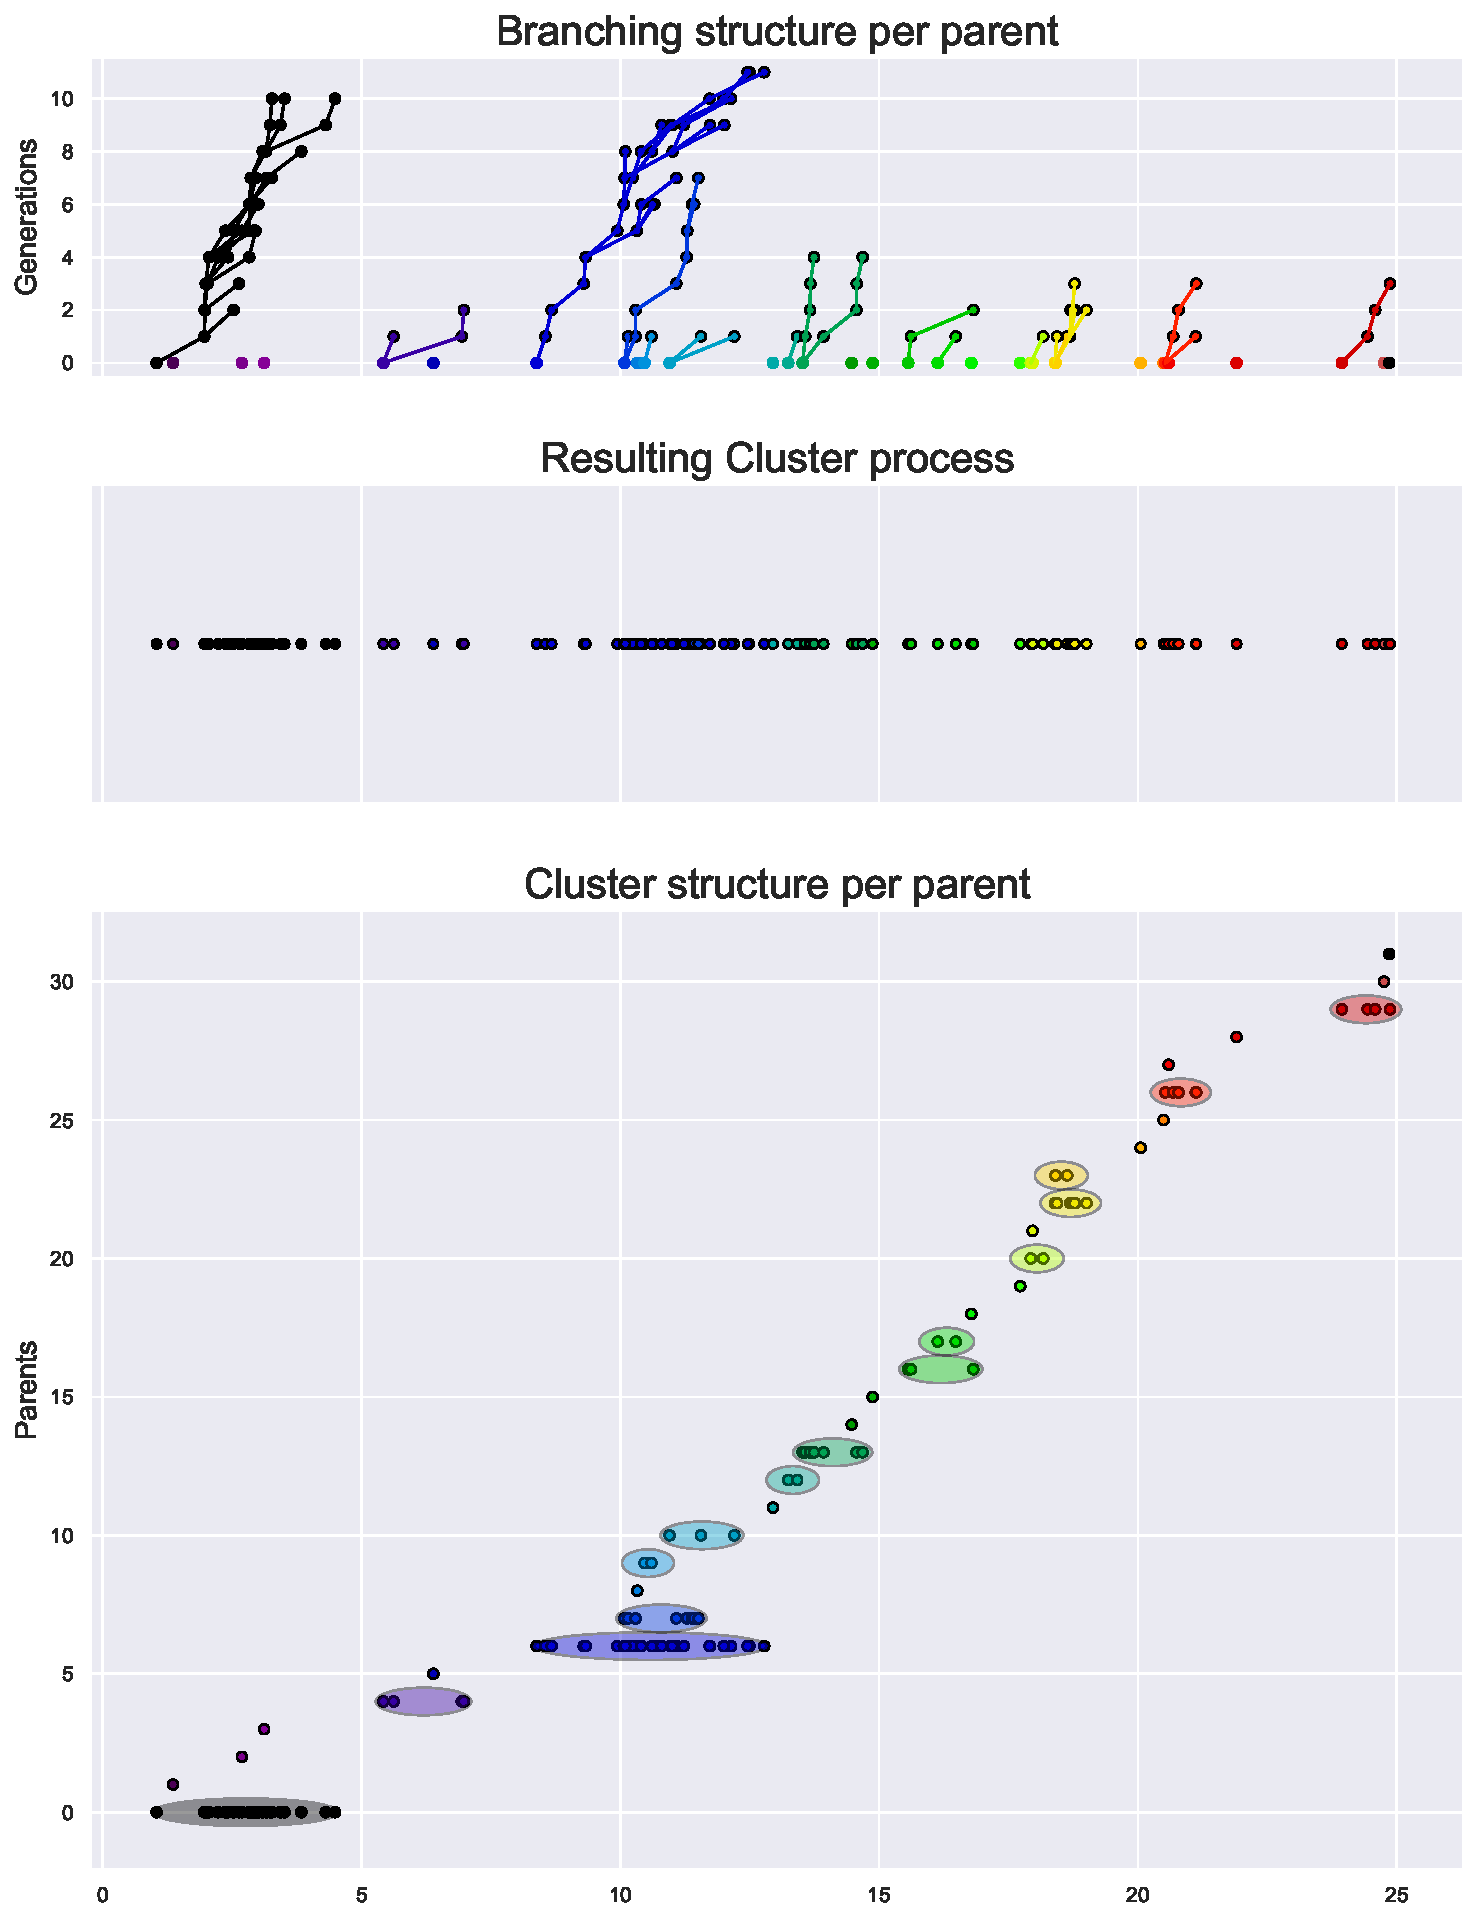
\includegraphics[width=0.95\textwidth]{images/chapter0/branching_and_cluster05.pdf}
      \caption{Illustration of both branching (top) and clustering (bottom) structures of an exponential Hawkes process (middle). Each color represents a single cluster/tree. Simulation is done through the cluster process algorithm.
      }
      \label{fig:branching_and_cluster05}
    \end{figure}

    From a numerical point of view, the definition of a Poisson cluster process as given above provides a simulation algorithm and an inference method from branching process theory was adapted to study Hawkes processes \parencite{Veen2008}.

    It is these properties, and the quick developments that followed in the literature, that created a growing interest in other scientific fields.
    From this, different versions of the original self-exciting Hawkes process appeared in the literature, each one trying to accomodate to more complex phenomena.

    \textbf{The multivariate Hawkes process.} Probably the most natural and useful is the definition of a \emph{multivariate} Hawkes process. 
    Instead of studying a single phenomenon (an univariate process), we define a $d$-variate Hawkes process as $d$ individual point processes $(N_i)_{i=1:d}$, 
    where each process is defined by a conditional intensity function $\lambda^i$:
    \[\lambda^i(t) = \mu_i + \sum_{j=1}^{d}\sum_{T_k^j \leq t}{h_{ij}(t-T_k^j)}\,, \qquad \text{for any $t\in\RR$.}\]

    In this formulation, each process $N_j$ has its own event times $(T_k^j)_{k\in\ZZ}$ and baseline intensity $\mu_j > 0$.
    This model introduces interaction between processes, which is seen in the second term of the intensity.
    The kernel functions $h_{ij}$ represent the effect of points from $N_j$ on process $N_i$.
    This model allows to study a group of individuals linked by a network of interactions, adding a new dimension of study for such processes.

    From modelling infection spread all the way to the study of clusters of earthquakes, approaching the study of Hawkes processes from a statistical point of view quickly became a necessity.

    \subsection{Inference and applications}

    \textbf{Statistical estimation.}
    %Presenting an exhausting bibliography on statistical estimation for Hawkes processes would represent a titanical task, 
    %specially due to the numerous alternative models introduced since their introduction.
    %Nonetheless, we propose here a general overview of the estimation panorama in the literature for self-exciting Hawkes processes.
    
    Statistical models for Hawkes processes with excitation focus around estimating both the baseline intenisty $\mu$ and the interation function $h$.
    In parametric settings, many kernel functions are traditionnally used (as some mentioned in the previous section),
    each one defined by a parameter $\gamma\in\RR^m$ for a certain integer $m$.

    %\Add theta and statistical model

    To our knowledge, the very first paper implementing an estimation procedure in a parametric framework is \textcite{Adamopoulos1976}.
    In his work, the author proposes a study of exponential kernels for both univariate and bivariate Hawkes processes through the spectral log-likelihood,
    closely related to time series theory.
    The exponential kernel is often chosen as a parametric interaction function because the univariate Hawkes process becomes a Markov process which presents the advantage of simplifying the expression of the intensity function. 
    This is exemplified in the implementation of the maximum likelihood estimator (MLE) in \textcite{Ozaki1979}.
    The expression of the log-likelihood of a general point process, for an observation in $[0, T]$, is:
    \begin{equation}\label{eq:chap0_loglikelihood}
      \ell_T(\theta) = - \int_{0}^{T}{\lambda(u)\,\dd u} + \sum_{k=1}^{N(T)}{\log(\lambda(T_k))}\,,
    \end{equation}
    where $N(T)$ is the number of points in the observation window. 
    Other estimation procedures in the parametric setting include \textcite{Ogata1988} for other kernel functions using the MLE, \textcite{Veen2008} as mentioned before by leveraging the branching structure, \textcite{Bacry2020} by minisiming a least-squares contrast, \textcite{DaFonseca2013} via the method of moments,

    The literature for inference in non-parametric setting is also vast with implementations of the MLE in \textcite{Guo2018} and penalised variant optimised by an Expectation-Maximisation algorithm.
    The least-squares minimisation is often used as shown in \parencite{Reynaud2010, Eichler2016, Kirchner2017}.
    Other methods include solving Wiener-Hopf equations \parencite{Bacry2016} or approximating the interaction functions with autoregressive models \parencite{Kirchner2017}.

    All of these references concern frequentist approaches of statistics, 
    and so it is essential to mention that an equal effort has been made from a Bayesian point of view.
    \textcite{Rasmussen2013} proposes two procedures through log-likelihood estimation: 
    one through the classical intensity function and another similar to \textcite{Veen2008} with the branching structure.
    In \textcite{Lemonnier2014}, the authors propose an approximation through exponential kernels and taking advantage of the markovian properties.
    The multivariate case is deeply study in \textcite{Donnet2020} with illustrations on estimating the underlying interaction graph.
    
    This is a small insight of the plethora of approaches that have been developed in order to study these kind of processes.
    
    \textbf{Applications and generalisations.}
    % The main motivation behind the works presented in this thesis, as it has been and continues to be for researches in this field,
    % is to use the versatility of the model and its exceptional adaptability to propose new submodels.
    % When confronted to real-world data, 
    % researchers tend to reformulate and complexify the Hawkes model in order to better describe the studied phenomena. 
    The temporal-dependancy structure of the Hawkes process has motivated its use accross a variety of application fields with many generalisations to obtain more explicative models.

    The historical example is the study of seismic activity where the occurrence of an earthquake is usually followed by a number of smaller tremors known as aftershocks.
    This behaviour is similar to the self-exciting effect modelled by the Hawkes process and associated to the clustering structure as shown in \textcite{Adamopoulos1976}.
    As in seismology the spatial placement and magnitude of each quake are important factors to take into account, applications on this field tend to include this information via the concept of marked point processes. 
    Each event time has an associated mark representing the detected magnitude \parencite{Ogata1988} and the location of each epicenter \parencite{Ogata1998, Kwon2023}.
    %Further develop

    A similar approach is done in the study of social media interactions for the analysis of subject trends.
    The excitation effect appears in the form of reposting where users have the option to share a news post among their followers which in turn may continue to spread the information in their social circles.
    In this context, the impact of each repost is dependant on the influence of the account and the impact of a topic on a certain community.
    This is represented for example by including account information in the form of number of followers \parencite{Mishra2016} again through marks, or by adding an additional dimension to the process \parencite{Pinto2015} to represent the impact of a topic over another.

    In criminology, it is commonly assumed that delinquent acts may incite other crimes in a population, which can be modelled by a self-exciting Hawkes process.
    As a branch of social sciences, it is important to account for different factors that affect human behaviour such as time of the day, demographics and social interactions.
    A way of accounting for this effects is to adapt the Hawkes process to time and spatial dependent baseline intensities. 
    A time-varying baseline intensity can represent periodic criminal behaviour \parencite{Lewis2011} with higher values for nightime.
    A space-dependant baseline is used to represent the link between residential density and burglary \parencite{Mohler2011} or the spatial distributions of gangs in a city \parencite{Linderman2014}.

    % Working in high dimensions allows to account for high number of individuals with sparse networks of interactions.
    % Penalisation methods in the study of neuronal spike trains \parencite{Reynaud2013, Lambert2018}
    % allow to reduce the support (non-null interactions) of the connectivity matrix.
    % This allows to improve estimations, allow for better computational times and more importantly provide more explicative models for the experts.

    Many other fields include finance \parencite{Embrechts2011, Bacry2013, Lotz2024}, genomics \parencite{Reynaud2010, Carstensen2010}, biology{Gupta2018, Denis2024, Nicvert2024}, epidemiology \parencite{Rizoiu2018, Chiang2022}, TV browsing behaviour \parencite{Xu2016}, event data streams in football \parencite{Baouan2023, Narayanan2023}, 
    each one often accompanied with new formulations of the Hawkes process.

    \subsection{Challenges and contributions}

    Our work in is motivated by the applications of Hawkes processes in neurobiology for the study of neuronal activity data.
    Neurons in the brain are connected through a deep network of synapses allowing them to communicate through electrical impulses usually studied by measuring the action potential or spikes emitted as the membrane potention of the cells are depolarised.
    These measurement generate a spike train of instants when a neuron activates and influences the membrane potential of connecting neighbours.

    These exchanges can appear either as excitatory or inhibitory to respectively incite or stop other neurons from activating.
    The first effect can be clearly modelled by a multivariate Hawkes process but the original modelling does not account for inhibiting effects.
    This requires in practice to allow for the interaction functions $h_{ij}$ to take negative values, introducing the concept of Hawkes processes with inhibition.

    In order to guarantee the non-negativity of the intensity function, a common practice in the literature is to consider the concept of \emph{non-linear Hawkes processes}.
    The main difficulty is that the branching structure of Hawkes processes is not valid anymore and the intensity function presents more complex behaviour so pre-established inference methods are not accessible anymore.
    The first part of this manuscript pertains to the study of inhibiting Hawkes processes in order to propose estimation methods in the parametric setting.
    We present an overview of the studied model and our contributions in Section~\ref{sec:chap0_inhibition}.
    
    The second part of this manuscript is focused around studying imperfect data.
    Collecting spike trains data is a procedure that can present measurement errors, which can appear as missing neuronal activation instants or by attributing spikes to the wrong neuron.

    This presents a common statistical framework of accounting for missing data in a sample of observations.
    In our context, not having a full knowledge on the past history of the process makes the conditional intensity function intractable.
    Our contributions, as summarised in Section~\ref{sec:chap0_missing_data}, are focused on exhibiting an inference paradigm through the spectral analysis of point processes for observations either noised by an external process or that are missing event times. 

    Although the models inbetween chapters may differ, our contribution follow a common thread by addressing the following four questions: 

    \begin{tcolorbox}
      \begin{itemize}
        \item What approaches can we take to establish parametric estimation procedures for more complex Hawkes processes dynamics?
        \item Under what conditions our statistical models are identifiable?
        \item How to evaluate and select the best estimators through data-driven methods?
        \item What modern statistical tools we can leverage to improve our inference procedures?
      \end{itemize}
    \end{tcolorbox}
    
    %These questions may serve as a general guide when reading this manuscript.

    %\subsection{Questions} %and contributions}
    % \begin{itemize}
    %     %\item In this thesis we study two extensions: 
    %     %\item In the first half (chapters) we study inhibition 
    %     %\item In the second half (chapters) we study missing data.
    %     \item Our studies are articulated along 3 general questions (i) what approaches for considering alternative or more complex dynamics than self-excitation in parametric and what properties can we establish; (ii) how to evaluate and select our models through data-based methods in multivariate cases (null interactions); (iii) what statistical tools allow us to improve inference.
    % \end{itemize}

% mentionner faire des outils accessible, partage du code (open source, facilité)
% mettre/valoriser les codes ici 

\section{Factoring in inhibition for Hawkes processes}\label{sec:chap0_inhibition}
    
    The original Hawkes process was proposed as a way of modelling the effect of excitation between points, which is characterised by the positivity of the interaction function $h$.
    Our first goal in this work is to study the opposite effect which is commonly known in the literature as \emph{inhibition}.
    
    An inhibiting Hawkes processes consists in modellling repulsion between points: each event will reduce the chances of others occurring for a certain period in time.
    Mathematically, a way of translating this effect is by allowing $h$ to take negative values. However, the non-negativity condition on $\lambda$ prevents us from taking this approach without adding some constraints.

    One of the most common solutions is the \emph{non-linear} Hawkes process model. In the univariate setting, let $h:\RR \to \RR$ and $\Phi:\RR\to\RR_{\geq 0}$ be two measurable functions. We define an univariate non-linear Hawkes process $N$ in the real half-line $\RR$ with event times $(T_k)_{k\in\NN}$ by the conditional intensity function, for any $t\in\RR$:
    \begin{equation}\label{eq:chap0_nonlinear_intensity}
      \lambda(t) = \Phi\left(\mu + \sum_{T_k \leq t}{h(t-T_k)}\right)\,.
    \end{equation}
    By allowing $h$ to be negative, the function $\Phi$ has to be a non-linear function. Existence of such processes is assured as long as $\Phi$ is an $L$-lipschitz function \parencite[Theorem 1]{Bremaud1996} such that:
    \[L\int_{0}^{+\infty}{\lvert h(t)\rvert\,\dd t} <1\,.\]
    Multiple choices exist in the literature like a clipped exponential function \parencite{Chornoboy1988,Carstensen2010,Gerhard2017}, a softplus function \parencite{Mei2017}, a sigmoid function \parencite{Menon2018}.
    
    In our work, we choose the positive part (ReLU) $\Phi(\cdot) = (\cdot)^+ = \max(0, \cdot)$ like in \textcite{Lemonnier2014, Hansen2015, Lu2018, Costa2020}.
    The intensity function (Equation~\eqref{eq:chap0_nonlinear_intensity}) becomes:
    \begin{equation}\label{eq:chap0_nonlinear_univariate_intensity}
      \lambda(t) = \left(\mu + \sum_{T_k \leq t}{h(t-T_k)}\right)^+\,,
    \end{equation}
    and the extension to a $d$-variate Hawkes process is:
    \begin{equation}\label{eq:chap0_nonlinear_multivariate_intensity}
      \lambda^i(t) = \left(\mu_i + \sum_{j=1}^{d}\sum_{T_k^j \leq t}{h(t-T_k^j)}\right)^+\,.
    \end{equation}

    Our general contribution in the context of Hawkes processes with inhibition is to provide parametric estimation procedures in a frequentist framework through maximum likelihood estimation.
    To our knowledge, and by the time of publication of both corresponding papers, other inference methods worked either in non-parametric \parencite{Reynaud2014,Bacry2016} or bayesian contexts \parencite{Rasmussen2013, Donnet2020, Sulem2021, Deutsch2022}.

    \subsection{Maximum Likelihood Estimation for Hawkes Processes with self-excitation or inhibition}
    
    In Chapter~\ref{chapter:univariate_inhibition}, we focus on the study of the univariate Hawkes process $N$ with intensity function described by Equation~\eqref{eq:chap0_nonlinear_univariate_intensity}.
    In order to establish the maximum likelihood estimator for a parametrised model of the intensity with parameter $\theta\in\Theta$, 
    it is necessary to obtain a closed-form expression of the log-likelihood:
    \[\ell_T(\theta) = - \int_{0}^{T}{\lambda_\theta(u)\,\dd u} + \sum_{k=1}^{N(T)}{\log(\lambda_\theta(T_k))}\,.\]
    
    For Hawkes processes with excitation, the linearity of the intensity function results in an explicit expression of $\ell_T$ without much trouble as shown in \textcite{Ozaki1979}.
    The main difficulty when including inhibition is that the cumulated effects from the past events may saturate process $N$, meaning that its intensity is null for a certain period in time.
    In the work of \textcite{Lemonnier2014}, the authors propose to approximate the computation in this context by ignoring the non-linear function.
    This allows them to circumvent this problem at the cost of assuming that the inhibition effects are small enough to be negligible.

    In order for us to obtain an exact computation of the loglikelihood that accounts for inhibition, we introduce two novel concepts: the \emph{underlying} intensity function $\lambda^\star$ and the \emph{restart times} $T_k^\star$.
    We define $\lambda^\star\colon \RR_{>0}\to \RR$, for any $t\leq 0$, as:
    \[\lambda^\star(t) = \mu + \sum_{T_k \leq t}{h(t-T_k)}\,,\]
    and the restart times $T_k^\star$ for any integer $k>0$ as:
    \[T_k^\star = \inf\{t\geq T_k \mid \lambda(t) > 0\}\,.\]

    The advantage of working with $\lambda^\star$ instead of $\lambda$ is that it inherits properties such as smoothness and strict monotony from the interaction function $h$ between any two consecutive event times $T_k$ and $T_{k+1}$.
    If assumed so, it follows that $T_k^\star$ is the moment from which both functions coincide.
    Our main contribution is providing a closed-form expresion of the compensator $\int_{0}^{T}{\lambda_\theta(u)\,\dd u}$, which we establish in Proposition~\ref{prop:chap0_integral_cooldown}.
    %establishing Proposition~\ref{prop:chap0_integral_cooldown}:
    %Our goal is to determine the values $t\geq 0$ such that $\lambda_\theta(t) > 0$ in order to exactly compute the compensator.
    \begin{proposition}\label{prop:chap0_integral_cooldown}
      For any $t>0$:
      
      \begin{equation}\label{eq:chap0_compensator_general}
      \int_{0}^{t}{\lambda(u)\,\dd u} =
      \begin{dcases}
          \mu t &\text{\qquad if $t<T_1$}\\
          \mu T_1 + \sum_{k=1}^{{N(t)-1}}{\int_{T_{k}^\star}^{T_{k+1}}{\lambda^\star(u)\,\mathrm{d}u}} + \int_{T_{N(t)}^\star}^{t}{\lambda^\star(u)\,\mathrm{d}u} &\text{\qquad if $t\geq T_1$}\,,
      \end{dcases}
      \end{equation}
      with the conventions that the sum is equal to $0$ if ${N(t)} = 1$ and the last integral is equal to $0$ if $t < T_{N(t)}^*$.

      If $h$ is the exponential kernel function, then the restart times read:
      \[
          T_k^\star = T_k + \beta^{-1} \log \left({\frac{\lambda_0 - \lambda^\star(T_k)}{\lambda_0}} \right) \II_{\lambda^\star(T_k) < 0}\,,
      \]
      and, for any integer $k\geq 1$ and any $\tau \in [T_{k}^*, T_{k+1}]$, each integral simplifies to 
      :
      \[
          \int_{T_{k}^\star}^{\tau}{\lambda^\star(u)\,\mathrm{d}u}
          = \lambda_0(\tau - T_{k}^\star) + \beta^{-1} (\lambda^\star(T_{k}) - \lambda_0) (\mathrm{e}^{-\beta(T_{k}^\star-T_{k})}-\mathrm{e}^{-\beta(\tau-T_{k})})\,.
      \]
      \end{proposition}

    This result allows to establish the maximum likelihood estimation procedure that accounts for both self-exciting and self-inhibiting effects, while keeping the same computational complexity as the method established in previous works. 
    In particular, for the exponential kernel function, the computational complexity of $\ell_T$ is $O(N(T))$ thanks to the Markovian property and as shown in our numerical study, the derived estimations are better than by using an approximation framework as presented in \textcite{Lemonnier2014} especially for high levels of inhibition effects.

    A second consequence of Proposition~\ref{prop:chap0_integral_cooldown} is that it gives access to a goodness-of-fit measure for our estimations by leveraging the Time Change theorem of point processes \parencite[Theorem 7.4.IV]{DaleyV1}.
    In particular, this allows to introduce a hypthesis testing procedure that evaluates the quality of our estimations on an independent set of observations.
    
    % With this result, it suffices to obtain a closed-form expression of the restart times, which we explicit in the case of the exponential kernel function.
    % We define then the maximum likelihood estimation procedure through an iterative algorithm to compute $\ell_T$.
    % An outstanding property of our approach is that it allows to account for both self-exciting and self-inhibiting effects, without increasing the computational complexity.

    % Our numerical study illustrates the efficiency of our estimator in multiple scenarios.
    % As expected, we demonstrate the importance of correctly accounting for inhibition in our estimation procedure. When compared to the approximation framework in \textcite{Lemonnier2014}, 
    % our approach provides better estimates in the exponential context, specially when the inhibition effects are consequential.
    % Finally, as a consequence of Proposition~\ref{prop:chap0_integral_cooldown}, we are able to implement a goodness-of-fit assessment of our models through the Time Change theorem of point processes \parencite[Theorem 7.4.IV]{DaleyV1}.
    % This allows to introduce a hypthesis testing procedure that allows to evaluate the quality of our estimations on an independent set of observations.





    \subsection{Inference of multivariate exponential Hawkes processes with inhibition and application to neuronal activity}
    Chapter~\ref{chapter:multivariate_inhibition} builds on the bases established in Chapter~\ref{chapter:univariate_inhibition} by adapting our estimation procedure to multivariate Hawkes processes $N = (N_1, \ldots, N_d)$. 
    In this setting the log-likelihood of $N$ reads:
    \[\ell_T = \sum_{i=1}^{d}{\left(- \int_{0}^{T}{\lambda_\theta^i(u)\,\dd u} + \sum_{k=1}^{N_i(T)}{\log(\lambda^i_\theta(T_k^i))} \right)}\,,\]
    where $\lambda^i$ and $(T_k^i)_k$ are respectively the intensity and event times of $N_i$.
    Similarly to the univariate case, we propose to study the underlying intensity functions $\lambda^{i\star}$:
    \[\lambda^{i\star}(t) = \mu_i + \sum_{j=1}^{d}\sum_{T_k^j \leq t}{h_{ij}(t-T_k^j)}\,,\]
    but this time the monotony condition of $h_{ij}$ is not enough to retrieve useful properties on this functions.

    This is a consequence of the increased complexity concerning the dynamics of each subprocess of allowing both exciting and inhibiting effects to exist simultaneously.
    In the multivariate setting, it is possible for a subprocess $N_i$ to be saturated ($\lambda(t)=0$) at an instant $t$ and to receive an external excitation of another subprocess.
    So, in order to simplify our problem, we restrict our study to the exponential kernel case $h_{ij}(t) = \alpha_{ij}\mathrm{e}^{-\beta_{ij} t}$ with the following mild assumption.

    \begin{assumption}\label{assu:chap0_beta}
      For each $i\in\{1,\ldots, d\}$, there exists $\beta_i\in\RR_+^*$ such that $\beta_{ij} = \beta_i$ for all $j\in\{1,\ldots, d\}$.
    \end{assumption}
    This allows us to recover the strict monotony of $\lambda^{i\star}$ between any two event times $T_{(k)}$ and $T_{(k+1)}$ of the general process $N$.
    With this, we adapt the expression of the restart times $(T_{(k)}^{i\star})_{k\geq 1}$ and the compensator $\int_{0}^{t}{\lambda^i(u)\,\mathrm{d}u}$ for each process $N_i$ and every event time $T_{(k)}$ allowing us to establish our first main contribution in the form of Propostion~\ref{prop:chap0_compensator}.

    \begin{proposition}\label{prop:chap0_compensator}
      Let us suppose that Assumption~\ref{assu:chap0_beta} is granted. 
      Then, for each $i\in\{1,\ldots, d\}$ and any $k\geq1$, we have:
      
      \begin{equation}\label{eq:chap3_restart_times_exponential}
        T\park^{i\star} = \min{\adaptedpar{t^\star_k, T\park[k+1]}}\,.
      \end{equation}
      where
      \[t^\star_k = \adaptedpar{T\park + \beta_i^{-1}\log{\adaptedpar{\frac{\mu_i - \lambda^{i\star}(T\park)}{\mu_i}}}\II_{\{\lambda^{i\star}(T\park) < 0\}}}\]
      And, for each $i\in\{1,\ldots, d\}$, the compensator of the process $N_i$ reads, $\forall t\geq 0$:
      \begin{equation}\label{eq:chap0_compensator_exponential}
        \int_{0}^{t}{\lambda^i(u)\,\mathrm{d}u} =
        \begin{cases}
          \mu_i t & \text{if } t < T\park[1] \\
          \mu_i T\park[1] + \sum_{k=1}^{N(t)} J_k & \text{if } t \geq T\park[1] \,,
        \end{cases}
      \end{equation}
      where for all integer \(k \in \{1, \dots, N(t)\}\):
      \begin{equation*}
        J_k =
        \mu_i \left[\min(t, T\park[k+1] ) - T\park^{i\star}\right] + \beta_i^{-1} \left(\lambda^{i\star}(T\park) - \mu_i \right)
        \left[ \mathrm{e}^{-\beta_i(T\park^{i\star} - T\park)} - \mathrm{e}^{-\beta_i(\min(t, T\park[k+1])- T\park)} \right]\,.
      \end{equation*}
      \end{proposition}

      With this result, we establish an exact procedure to compute the log-likelihood $\ell_T^i$ of each process $N_i$, giving us access to the complete log-likelihood $\ell_T$ and in turn, access to the maximum likelihood estimation method.
      Let us note that as in the univariate case, we also get access to a goodness-of-fit procedure via the Time Change theorem.
      
      Another complication brought upon by the multivariate setting is that the identifiability of our statistical model for the exponential Hawkes process is not as evident as in the univariate case.
      To partially answer this question, we provide an observational sufficient condition in Theorem~\ref{th:chap0_identifiability} that allows to ensure an identifiable model, which ensures that our estimation procedure can be correctly implemented

      \begin{theorem}[Identifiability]\label{th:chap0_identifiability}
        For all $i=1\colon d$, let $\theta_i \in \Theta$ be a parameter for $\lambda^i$.

        Let us assume that a.s. for every $(i, j) \in \{1, \dots, d\}^2$, $i\neq j$,
        there exist an event time \(\tau\) from process \(N^j\),
        and an event time \(\tau_+ > \tau\) from process \(N^i\), such that:
        \begin{enumerate}
            \item $\lambda_{\theta_i}^i(\tau^-) > 0$;
            \item There are only events of process $N^j$ in the interval $[\tau, \tau_+)$.
        \end{enumerate} 
        
        Then,
        \[
          \forall i \in \{1, \dots, d\},~
          \lambda_{\theta_i}^i(t) = \lambda_{\theta_i'}^i(t) \text{ a.e.}
          \qquad
          \iff
          \qquad
          \forall i \in \{1, \dots, d\},~\theta_i = \theta'_i\,.
        \]
    \end{theorem}

      Overall, this condition allows to avoid pathological situations either where some process $N_i$ is not observed (strong external inhibition effects), or there is a cyclical observation of points (strong internal inhibition effects).

      Finally, we present a solution for the estimation of the interaction network of a multivariate Hawkes process.
      As it is common in real-data contexts, it is often unrealistic to assume that all functions $h_{ij}$ are non-null, meaning that all processes interacts with each other.
      For this, we propose three different data-driven techniques based on a thresholding approach inspired by principal component analysis, and based on the construction of confidence intervals (student and empirical).
      Our results on synthetic data show a significant improvement with respect to other state-of-the-art methods \parencite{Lemonnier2014, Bacry2020}.
      In particular, when the interaction matrix $(\alpha_{ij})_{i,j=1:d}$ contains null entries, we implement our post-hoc procedures to obtain an estimation of the connectivity network before re-estimating all non-null entries on a reduced model.
      This provides the best estimations of all parameters among the considered models, as confirmed by our results on real-data concerning the analysis of neuronal activity.

      % Finally, we provide some insights on the performance of our procedures in both simulated and real-world contexts.
      % The results for the simulated samples show a significant improvement with respect to other state-of-the-art methods \parencite{Lemonnier2014, Bacry2020}.
      % In particular, when the interaction matrix $(\alpha_{ij})_{i,j=1:d}$ contains null entries, we implement our post-hoc procedures to obtain an estimation of the connectivity network before re-estimating all non-null entries on a reduced model.
      % This provides the best estimations among all considered models.
      
      %In the context of real data, we study ten samples of neuronal activity between 223 neurons of a red-eared turtle.
      % This dataset represents a difficult task for any kind of estimation method. In order to improve our estimators we resort to a resampling technique proposed in \textcite{Reynaud2014}.
      % Furthemore, we implement as in the univariate case a goodness-of-fit procedure accessed once again via the time change theorem.
      % This is an important step in order to compare the quality of all models as we have no prior information on the real interaction network.
      % To account for the high dimensionality, we incorporate a multiple testing procedure, which establishes our estimation through empirical confidence intervals as the best fitting model.

    % By allowing the interaction function $h$ to take negative values,
    % the occurrence of a point \emph{decreases} the rate of incoming event times.
    % The main difficulty of this approach originates from the non-negativity requirement on the conditional intensity function.
    % This is often controlled by introducing the concept of \emph{non-linear} Hawkes processes.



\section{Something is amiss: spectral methods for imperfect data}\label{sec:chap0_missing_data}
    
  In the second part of the thesis, we turn the spotlight to a common issue in statistics: 
  establishing efficient estimation procedures when the observed data is noised in some sense.

  In the context of point processes, a natural approach to define noised models is through the operations of thinning, superposition and jittering.
  These are mathematical transformations that allow to obtain new point processes through these different mechanisms:
  \begin{enumerate}
    \item The \textbf{superposition} of two point processes $X$ and $Y$, usually noted $X+Y$ is the point process defined by the ordered union of event times $T_k^X$ and $T_k^Y$.
    \item The \textbf{thinning} of a point process corresponds to erasing event times $T_k^X$ of a point process $X$ through a random rule.
    When point are erased independently from each other with a common probability $1-p$, we talk about a $p$-thinning of process $X$.
    \item \textbf{Jittering} a point process consists in the random displacement of points through the means of a probability distribution.
  \end{enumerate}

  The main interest of studying such alterations is to account for various measurement errors in real-world data. 
  The most commonly studied in the literature is jittering which tends to appear when spatial imprecisions add a layer of uncertainty, as in \parencite{Bonnet2022}. 
  Literature tends to focus on Poisson processes \parencite{Antoniadis2006, Hohage2016},
  with Hawkes processes being studied in \parencite{Trouleau2019, Deutsch2020}.

  Thinning is often used to represent missing data but has been scarcely studied in the literature. \textcite{Mei2019} propose a method to complete a sequence of times that have missing points via an LSTM model based on the Hawkes process.
  
  The study of superposition allows to account for observations that are contaminated by points originated from an external process, but are indistinguishable from those of the original process. 
  To our knowledge, the only work who studies this kind of noise is \textcite{Lund2000}, which in fact studies a general point process that is potentially noised by the three aforementioned mechanisms.
  Their work establishes an approach by maximising the conditional log-likelihood dependent on the original process with an application to Hawkes processes.
  In practice and for numerical reasons, they propose a local maximiser of this quantity in a small set of parameter when having acccess to an estimation of the unnoised process.

  Other imperfect data models have been presented in \textcite{Linderman2014} in the form of missing marks, intervals or entire processes, where the authors favour a Bayesian approach through latent variables. 
  The last work we mention here is the work by \textcite{Cheysson2022}, where the exact position of the points of a Hawkes process are not known. 
  Instead, the only information available is the number of points that fall inside equally-sized intervals.
  They leverage then the spectral theory of point processes and time series in order to provide an estimation procedure that does not necessitate the precise location of event times.
  
  Our contribution is to make use of the spectral theory of point processes, centered around the Bartlett spectrum \parencite{Bartlett1964} and the Whittle estimator \parencite{Whittle1952}, in order to propose estimators fo noised versions of the Hawkes process through superposition (Chapter~\ref{chapter:spectral_superposition}) and thinning (Chapter~\ref{chapter:spectral_thinning}).
  Another contribution is to leverage the obtained inference method to incorporate a subsampling paradigm through thinning for small observation windows.
  The existing spectral theory for Hawkes processes is limited to exciting interactions, so we restrain our models to this framework.
  
  
    %\begin{itemize}
    %    \item Introduce the point process operations and provide missing data formalism. 
    %    \item Bibliography
    %\end{itemize}




    \subsection{Spectral analysis for the inference of noisy Hawkes processes}
    Chapter~\ref{chapter:spectral_superposition} is consacrated to the study of the superposition of a Hawkes process $H$ with exciting kernel functions and an independent homogeneous Poisson process $P$ with intensity $\lambda_0 > 0$.
    We consider the superposition of both processes, that we note $N = H + P$,
    and we assume that we have no prior knowledge on the origin of each event time $T_k^N$ (either Hawkes or Poisson).
    The intensity function of this resulting process is intractable and so any method based on it is innaccessible as a consequence. 
    
    As mentioned previously, we take inspiration from \textcite{Cheysson2022} in order to leverage the spectral approach of point processes to circumvent this issue. 
    The Bartlett spectrum $\Gamma^N$ of $N$ is a measure defined by the means of the Fourier transform of its reduced covariance measure.
    When this measure is absolutely continuous, its density is noted $f^N$ and often called the spectral density of the process.
    We can establish an estimation procedure of a parametric model for $f^N$ with parameter $\theta\in\Theta$ through the periodogram funciton $I^T$.
    For an observation $(T_k^N)_{k\geq 1}$ in $[0,T]$, the periodogram is defined, for any $\omega\in\RR$, as:
    \begin{equation}\label{eq:chap0_periodogram}
      I^T(\omega) = \frac{1}{T}\sum_{k=1}^{N(T)}\sum_{l=1}^{N(T)}{\mathrm{e}^{-2\pi \iu \omega (T_k^N - T_l^N)}}\,.
    \end{equation}
    Asymptotically, this quantity follows an exponential distribution of mean $f(\omega)$ and so it is possible to define the maximum spectral log-likelihood estimator $\hat \theta$ as:
    \begin{equation}\label{eq:chap0_spectral_estimator}
      \hat \theta = {\arg\max}_{\theta\in\Theta} \left(-\frac{1}{T}\sum_{k=1}^{M}{\left(\log\left(f_\theta^N(\omega_k)\right) + \frac{I^T(\omega_k)}{f_\theta^N(\omega_k)}\right)}\right)\,,
    \end{equation}
    where $\omega_k = k/T$ for $k=1:M$.
    What makes this quantity so useful in our context is that it can be exactly computed without any information of the source of event times $(T_k^N)_k$. 

    Our first results establishes the expression of the spectral density function for the superposition of two independent point processes as exhibited in Proposition~\ref{prop:chap0_sum_of_spectral_densities}.

    \begin{proposition}\label{prop:chap0_sum_of_spectral_densities}
      Let $X$ and $Y$ be two independent and stationary point processes, admitting respective spectral densities ${f}^X$ and ${f}^Y$.
      
      Then $N = X + Y$ admits a spectral density function $f^N$ and
      \begin{equation} \label{eq:chap0_sum_spectral_densities}
        {f}^N = {f}^X + {f}^Y\,.
      \end{equation}
    \end{proposition}
    As the spectral density of a Hawkes process is explicit \parencite[Example 8.2(e)]{DaleyV1}, we obtain the general form of the spectral density of our noisy Hawkes process $N$ in order to establish an estimation procedure by maximising the spectral log-likelihood.

    %To correctly work with these tools, it is necessary to consider stationary point processes,
    %which for the case of Hawkes processes necessitates to consider processes in the entire real line $\RR$.
    
    Our main contribution in the univariate setting is to establish conditions for the identifiability of $f^N$ for different parametrisations of the kernel function $h$. 
    The first result concerns the classic exponential kernel. 
    We show that the model is identifiable if and only if one of the four parameters (three for the Hawkes process and one for the Poisson process) is fixed, even though the distribution of $N$ is uniquely determined without this constraint.
    Furthermore, we prove that the noisy Hawkes process with an uniform kernel function defines an identifiable spectral model.
    %We also prove that the noisy Hawkes process with an uniform kernel function defines an identifiable spectral model, which suggests that the non-identifiability issues is not  the spectral approach.
    %The non-identifiability derives then from the spectral approach and not from the superposition operation, as for a noisy Hawkes process with uniform interaction functions the model is identifiable
    %In order to determine whether the non-identifiability is due to the spectral approach or not, we study the noisy Hawkes process with uniform kernel and show that the spectral model is identifiable

    In the multivariate case, all tools from spectral theory exist and results are easily extended concerning the estimation procedure.
    Our contributions concern specifically the bivariate exponential Hawkes process noised this time by a bivariate Poisson process with common parameter $\lambda_0$.
    We present condition on the interaction matrix $(\alpha_{ij})_{1 \leq i,j \leq 2}$ that characterise either the identifiability or non-identifiability of the corresponding statistical model.

    Our work is concluded by a numerical study in both the univariate and bivariate cases when identifiability conditions are verified.
    We show in both cases that our estimators perform particularly well, specially for processes with strong excitation effects and as the observation horizon $T$ increases.
    Our final contribution is to propose an ad-hoc procedure in the bivariate case that allows to determine the support of the interaction matrix by considering the empirical 5$\%$ quantiles of a sample of estimations, which in turn enhances the performance of our methods.
    




    \subsection{A numerical exploration of thinned Hawkes processes through spectral theory}
    The last Chapter~\ref{chapter:spectral_thinning} turns to the analysis of the thinning operation for point processes.
    Let $H_p$ be a process issued from thinning an univariate Hawkes process with a probability $1-p$ of erasing each point $T_k$, for $k\in\ZZ$.
    As previously mentioned, any method based on the conditional intensity function is unavailable, so we turn to spectral theory.

    All the tools presented in the previous subsection can still be implemented here, in particular the expression of the periodogram (Equation~\eqref{eq:chap0_periodogram}) remains unchanged. 
    As a consequence, it can still be exactly computed even though we do not observe all points of the original process.
    In order to implement an inference procedure as defined by Equation~\eqref{eq:chap0_spectral_estimator}, we need to obtain an expression of the $p$-thinned process $H_p$.
    This is obtained in Proposition~\ref{prop:chap0_spectral_thinning}.

    \begin{proposition}\label{prop:chap0_spectral_thinning}
      Let $H$ be a stationary point process admitting a spectral density function $f^H$ and let $m_1=\EE[\lambda(t)]$ be its average intensity.
      For any $p\in(0,1]$, let $H_p$ be a $p$-thinning of $H$.
  
      Then, $H_p$ admits a spectral density function, denoted $f^{H_p}$, such that for any $\omega\in\RR$:
      \begin{equation}\label{eq:chap0_spectral_thinning}
          f^{H_p}(\omega) = p^2 f^H(\omega) + p(1-p)m_1\,.
      \end{equation}
  
  \end{proposition}
    This result is obtained by leveraging the spectral theory of marked point processes as presented in \textcite{Bremaud2005}.

    We focus our study on the exponential kernel function and we prove that the derived statistical model is identifiable if and only if one parameter is fixed, similar to the superposition scenario.
    We present numerical results under this condition by fixing the value of the thinning parameter $p$. 
    In particular, we show that our estimation method is robust with respect to the level of thinning, with remarkable results when enough event times are available for inference.
    This is particularly encouraging, as the thinning procedure can dilute the interactions between the original points from process $H$.
    
    Our last contribution in this work is to make use of the thinning operation as a subsampling procedure when a single observation of $H$ is available in a small window of time.
    The use of subsampling for point processes has been done previously in the literature \parencite{Moller2003, Cronie2024} in order to improve estimation procedures.
    In our case, we focus on enhancing the quality of our spectral estimations by combining an $\ell_2$ penalisation with an averaged estimator obtained by thinning the unique observation of $H$.
    We show that our proposed procedure provides in general the best estimations when compared to another subsampling procedure and displays a net improvement of the relative $\ell_2$ error by reducing the high bias observed for the non-penalised estimator.
    
\section{Outline of the manuscript.}\label{sec:chap0_outline}

    This manuscript is divided in two parts, with Chapter~\ref{chapter:background} presenting a succinct presentation of point processes theory, from a random measure approach, and the formalism of Hawkes processes.
    Let us note that all chapters are independent of each other and can be read as standalone documents.

    The first part of this thesis (Section~\ref{sec:chap0_inhibition}) concerns the study of the inhibition: 
    the opposite effect to excitation.

    \begin{itemize}
      \item Chapter~\ref{chapter:univariate_inhibition} presents a parametric estimation method for univariate Hawkes processes that accounts for both self-exciting or self-inhibiting interactions. 
      This is a joint work with Anna Bonnet and Maxime Sangnier. 

      The corresponding paper \parencite{bonnet2021} has been published in \textit{Statistics and Probability Letters}.
      
      Code is freely available at \url{https://github.com/migmtz/hawkes-inhibition-expon}

      \item Chapter~\ref{chapter:multivariate_inhibition} presents a parametric estimation method for multivariate exponential Hawkes processes with exciting and inhibiting interactions along with a model selection procedure. 
      This is a joint work with Anna Bonnet and Maxime Sangnier. 

      The corresponding paper \parencite{Bonnet2023} has been published in \textit{Statistics and Computing}.
      
      Code is freely available at \url{https://github.com/migmtz/multivariate-hawkes-inhibition}

    \end{itemize}

    The second part (Section~\ref{sec:chap0_missing_data}) consists in the study of imperfect observations of a Hawkes process realisation, similar to missing data formulations.

    \begin{itemize}
      \item Chapter~\ref{chapter:spectral_superposition} presents a parametric estimation method for exciting Hawkes processes whose event times are noised by those of a homogenenous point process, leveraging point process spectral theory. 
      This is a joint work with Anna Bonnet, Felix Cheysson and Maxime Sangnier. 

      The corresponding paper \parencite{Bonnet2024} has been submitted for publication.

      Code is available at \url{https://github.com/migmtz/noisy-hawkes-process}

      \item Chapter~\ref{chapter:spectral_thinning} presents the analysis of an inference method for thinned univariate Hawkes processes through spectral theory. 
      Additionally, it presents an improvement of $\ell_2$ penalisation through thinning subsampling for the spectral estimator.

      This chapter is an ongoing joint work with Felix Cheysson.
    \end{itemize}




%\section{The numerical contributions}

%entrer titre et outline

% Application que en 2 mais dire que l'on essaye de le garder en tete dans nos etudes

\leadchapter{
  In this paper, we present a maximum likelihood method for estimating the parameters of a univariate Hawkes process with self-excitation or inhibition. 
  Our work generalizes techniques and results that were restricted to the self-exciting scenario.
  The proposed estimator is implemented for the classical exponential kernel and we show that, 
  in the inhibition context, our procedure provides more accurate estimations than current alternative approaches.
}

\chapter[][MLE for Hawkes Processes with self-excitation or inhibition]{Maximum Likelihood Estimation for Hawkes Processes with self-excitation or inhibition}\label{chapter:univariate_inhibition}

% sec, eq, prop, alg, th, cor, def, fig, app, table

% 

\section{Introduction}

The Hawkes model is a point process observed on the real line, which generally corresponds to the time, where any previously encountered event has a direct influence on the chances of future events occurring. This past-dependent mathematical model was introduced in \textcite{Hawkes1971} and its first application was to model earthquakes occurrences \parencite{Ogata1988, Ogata1998}. Since then, Hawkes processes have been widely used in various fields, for instance finance \parencite{Bacry2013}, social media \parencite{Rizoiu2017, Mishra2016}, epidemiology \parencite{Rizoiu2018}, sociology \parencite{Linderman2014} and neuroscience \parencite{Reynaud2014}.

The main advantage of Hawkes processes is their ability to model different kinds of relationships between phenomena through an unknown kernel or transfer function. The Hawkes model was originally introduced as a self-exciting point process where the appearance of an event increases the chances of another one triggering.
Several estimation procedures have been proposed for the kernel function, both in parametric \parencite{Ogata1988, DaFonseca2013, Ozaki1979} and nonparametric \parencite{Reynaud2014, Bacry2016} frameworks.

However, the inhibition setting, where the presence of an event decreases the chance of another occurring, has drawn less attention in the literature, although it can be of great interest in several fields, in particular in neuroscience \parencite{Lambert2018}. In this inhibition context, the cluster representation \parencite{Hawkes1974} on which is based the construction of a self-exciting Hawkes process, is no longer valid.
While the existence and the construction of such nonlinear processes can be found in recent works for the univariate \parencite{Costa2020} and multivariate \parencite{Chen2017} cases,
statistical estimation of the kernel function has been hardly addressed.
A first approach consists in computing an approximation of the likelihood as if the intensity function could take negative values, and optimizing it to get a maximum likelihood estimator \parencite{Lemonnier2014}.
Alternatively, the type of interaction (excitation or inhibition) can be considered as a hidden variable, giving rise to a very practical estimation method \parencite{Mei2017}.

In this paper, we propose a maximum likelihood procedure that can handle both excitation and inhibition scenarios for a univariate Hawkes process. Our approach is based on an explicit computation of the likelihood for any type of monotone kernel functions, which is facilitated by the introduction of the natural concept of restart points. The latter are the times when the intensity function, that can be null on some intervals, become strictly positive again. We show that these restart points have a closed-form expression when the kernel is exponential, which allows us to rewrite and maximize the likelihood without approximations that are proposed for instance in \textcite{Lemonnier2014}.  Our estimator is implemented in Python (the code is freely available online\footnote{\url{https://github.com/migmtz/hawkes-inhibition-expon}}). We also propose a numerical study which shows the good performance of our exact estimation procedure compared to approximated approaches, especially when the intensity function is frequently equal to zero.

To outline the paper, besides a quick introduction to self-regulating Hawkes processes (also referred to as self-correcting Hawkes processes or Hawkes processes with inhibition), Section~\ref{sec:chap1_general} introduces the concepts of underlying intensity function and restart points.
General results concerning the compensator and the exact maximum likelihood estimation procedure are described in Section~\ref{sec:chap1_mle}.
At last, after a brief discussion about goodness-of-fit in Section~\ref{sec:chap1_goodness},
Section~\ref{sec:chap1_num_res} concludes with a numerical study of the estimation error.

\section{The Hawkes process}\label{sec:chap1_general}

Let $N$ be a point process on $\RR_+^*$, here \(\RR_+^* = \left\{ x>0 : x \in \RR \right\}\), and $(T_k)_{k\geq 1}$ its associated event times (with convention $T_0 = 0$).
For any $t \geq 0$, let us note $N(t) = \sum_{k\geq 1}{\II_{T_k \leq t }}$ the number of events in $[0,t]$
(where \(\II_{\cdot}\) stands for the indicator function),
and $\lambda$ its conditional intensity function \parencite{DaleyV1}:
\begin{equation*}
    \lambda(t) = \lim_{h\to 0}{\frac{\PP(N(t+h) - N(t) > 0)}{h}}\,.
\end{equation*}

A univariate Hawkes process is a point process defined by the conditional intensity function:
\begin{align}
    \lambda(t) &= \left(\lambda_0 + \int_{0}^{t}{h(t-s)\,\mathrm{d}N(s)}\right)^+
    = \left(\lambda_0 + \sum_{T_k \leq t}{h(t-T_k)}\right)^+\,,
    \label{eq:chap1_general_hawkes}
\end{align}
where $x^+ = \max(0,x)$ denotes the positive part of any real value $x$,
$\lambda_0\in\RR_+^*$ is the baseline intensity and
\(h : \RR_+ \to \RR\) is the kernel, which is assumed to be a monotone measurable function with $\lim_{t\to\infty} h(t) = 0$.
The kernel function $h$ is the key component of a Hawkes process:
it translates the influence (generally assumed to fade away over time) of a past event over the process.
Here, $h$ is allowed to take negative values, meaning that it can model both self-exciting and self-regulating Hawkes processes.

Working with such Hawkes processes may prove to be difficult as the positive part function is non-linear.
In particular, while computing the compensator function \parencite{DaleyV1}
\begin{equation}
    \Lambda(t) = \int_{0}^{t}{\lambda(t)\,\mathrm{d}t}\,,
    \quad \forall t \geq 0,
    \label{eq:chap1_compensator}
\end{equation}
is very easy in the self-exciting case (by linearity of the intensity), it becomes more challenging for the self-regulating Hawkes process.
As it is the keystone to derive the likelihood function (and then to obtain a parametric estimation method), our first contribution is to provide an exact expression of the compensator.

For this purpose, let us first introduce the \emph{underlying intensity function} and the \emph{restart time}, two quantities which will allow us to
derive the computation of the likelihood of a monotone Hawkes process, in a framework unifying self-correcting and self-exciting Hawkes processes.

\begin{definition}
Let the \emph{underlying intensity function} of $N$ be:
\begin{equation*}
    \lambda^\star(t) = \lambda_0 + \int_{0}^{t}{h(t-s)\,\mathrm{d}N(s)}\,.
\end{equation*}

In addition, let the \emph{restart time} $T_k^\star$ be, for any positive integer $k$:
\begin{equation*}
    T_k^\star = \inf{\{t\geq T_k\mid \lambda(t) > 0\}}\,,
\end{equation*}
along with its corresponding \emph{cooldown interval} $\tau_k^* = T_k^* - T_k$.
\label{def:chap1_underlying}
\end{definition}

\begin{figure}[!ht]
  \centering
  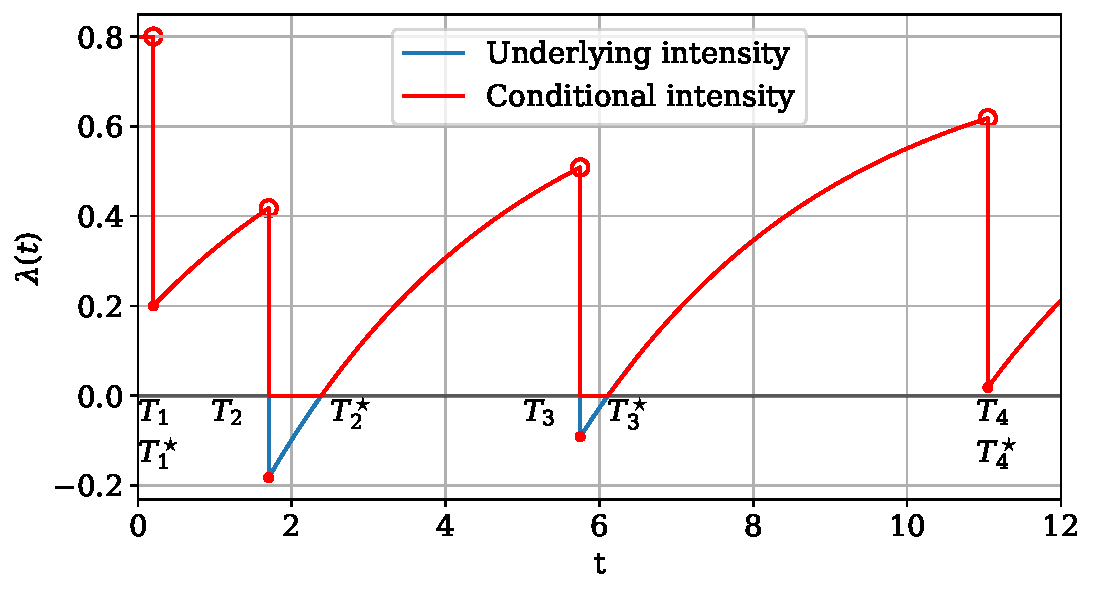
\includegraphics[width=0.7\textwidth]{images/chapter2/cooldownTimesMarkedSerif2.pdf}  % Previously 0.7
  \caption{Example of the intensity (red curve) and underlying intensity (blue curve) for a self-regulating Hawkes process, with the associated restart times. We only see the negative values of the blue curve since they precisely correspond to the values for which the two intensity functions are not equal.
  }
  \label{fig:chap1_underlying_intensity}
\end{figure}

As illustrated in Figure \ref{fig:chap1_underlying_intensity}, $\lambda^\star$ corresponds to the intensity $\lambda$ as if it were allowed to take negative values.
Moreover, as the kernel is assumed to be monotone, the restart time associated to one occurrence can be interpreted as the first moment after this occurrence from which $\lambda$ and $\lambda^\star$ become equal  (in particular, the restart time and the occurrence time coincide if the intensity function is nonnegative at this time, see Figure \ref{fig:chap1_underlying_intensity}):
\begin{equation*}
    T_k^\star = \inf{\{t\geq T_i\mid \forall t\in(T_k^*,T_{k+1}),\, \lambda(t) = \lambda^\star(t)\}}\,.
\end{equation*}

\section{Maximum likelihood estimation and the exponential model}
\label{sec:chap1_mle}

Assume a parametric model $\mathcal P = \left\{ \lambda_\theta, \theta \in \Theta \right\}$ for the conditional intensity function $\lambda$, where $\theta$ contains unknown quantities such as the baseline $\lambda_0$ and the kernel $h$.
Then, with convention $log(t) = -\infty$ for $t\leq0$, the log-likelihood $\ell_t$ of any $\theta \in \Theta$ with respect to the observations $T_1,\ldots, T_{N(t)}$ in the time interval $[0,t]$ is \parencite[Proposition 7.2.III.]{DaleyV1}, \parencite{Ozaki1979}:
\begin{equation}\label{eq:chap1_log_likelihood}
    \ell_t(\theta) = \sum_{k=1}^{N(t)}{\log{(\lambda_\theta(T_k^-))}} - \Lambda_\theta(t)\,,
\end{equation}
where the compensator $\Lambda_\theta$ is defined as in Equation \eqref{eq:chap1_compensator} and $\lambda_\theta(T_k^-) = \lim_{t \to T_k^-} \lambda_\theta(t)$.

Equation~\eqref{eq:chap1_log_likelihood} reveals the importance of being able to compute the compensator $\Lambda$ (equivalently $\Lambda_\theta$) in order to provide a practical implementation of the maximum likelihood estimator of $\lambda$.
Thus, a first contribution of this paper lies in Proposition~\ref{prop:chap1_integral_cooldown}, which establishes a decomposition of the compensator $\Lambda$ using the underlying intensity function $\lambda^\star$ and the restart times $T_{1}^\star,\ldots, T_{N(t)}^\star$.

\begin{proposition}\label{prop:chap1_integral_cooldown}
For any $t>0$, the compensator $\Lambda$ can be expressed as:

\begin{equation}\label{eq:chap1_compensator_general}
\Lambda(t) =
\begin{dcases}
    \lambda_0 t &\text{\qquad if $t<T_1$}\\
    \lambda_0 T_1 + \sum_{k=1}^{{N(t)-1}}{\int_{T_{k}^\star}^{T_{k+1}}{\lambda^\star(u)\,\mathrm{d}u}} + \int_{T_{N(t)}^\star}^{t}{\lambda^\star(u)\,\mathrm{d}u} &\text{\qquad if $t\geq T_1$}\,,
\end{dcases}
\end{equation}
with the conventions that the sum is equal to $0$ if ${N(t)} = 1$ and the last integral is equal to $0$ if $t < T_{N(t)}^*$.
\end{proposition}
\begin{proof}
This comes directly from splitting the integral of $\Lambda(t) = \int_{0}^{t}{\lambda(t)\,\mathrm{d}t}$ on the intervals $[T_k, T_{k+1})$ ($k \in \{ 0, \dots, N(t)-1 \}$) and $[T_{N(t)}, t]$, and by remarking that, since $h$ is monotone, $\forall t\in[T_k, T_{k+1})$, $\lambda(t) = \lambda^\star(t)\II_{[T_k^*,T_{k+1})}(t)$.

\end{proof}

In order to give an explicit computation of the quantity $\int_{T_{k}^\star}^{T_{k+1}}{\lambda^\star(u)\,\mathrm{d}u}$ (equivalently $\int_{T_{N(t)}^\star}^{t}{\lambda^\star(u)\,\mathrm{d}u}$) which appears in Proposition~\ref{prop:chap1_integral_cooldown}, we focus on the classical scenario where we consider an exponential kernel $h(t) = \alpha \mathrm{e}^{-\beta t}$, for some $\alpha\in\RR$ and $\beta\in\RR_+^*$.
Let us notice that $\alpha$ can be either positive or negative, meaning that the process may be either self-exciting or self-regulating.

Then, the underlying intensity function can be written as:
\begin{equation}\label{eq:chap1_exponential_intensity}
    \lambda^\star(t) = \lambda_0 + \int_{0}^{t}{\alpha \mathrm{e}^{-\beta(t-s)}\,\mathrm{d}N(s)}\,.
\end{equation}
The forthcoming proposition steps forward in computing the compensator for an exponential kernel.

\begin{proposition}[Compensator for exponential kernel]
Let $t > 0$ and $k \in \{1, \dots, N(t)\}$.
The restart times read:
\[
    T_k^\star = T_k + \beta^{-1} \log \left({\frac{\lambda_0 - \lambda^\star(T_k)}{\lambda_0}} \right) \II_{\lambda^\star(T_k) < 0}\,,
\]
and the compensator is expressed as in Equation~\eqref{eq:chap1_compensator_general}, with,
for any $\tau \in [T_{k}^*, T_{k+1}]$:
\[
    \int_{T_{k}^\star}^{\tau}{\lambda^\star(u)\,\mathrm{d}u}
    = \lambda_0(\tau - T_{k}^\star) + \beta^{-1} (\lambda^\star(T_{k}) - \lambda_0) (\mathrm{e}^{-\beta(T_{k}^\star-T_{k})}-\mathrm{e}^{-\beta(\tau-T_{k})})\,.
\]

\label{prop:chap1_exp}
\end{proposition}
\begin{proof}
The proof is in \ref{app:chap1_appendix}.
\end{proof}

\begin{corollary}[Log-likelihood for exponential kernel]
  Let
  \begin{equation}
    \mathcal P = \left\{ \lambda_\theta = \bar{\lambda_0} + \int_{0}^{t}{\bar \alpha \mathrm{e}^{-\bar \beta(t-s)}\,\mathrm{d}N(s)} : \theta=(\bar{\lambda_0}, \bar \alpha, \bar \beta) \in \Theta \right\}\,,
    \label{eq:chap1_model}
  \end{equation}
  be a parametric exponential model for the conditional intensity function $\lambda$ with $\Theta = \RR_+^* \times \RR \times \RR_+^*$,
  along with the candidate compensator $\Lambda_\theta$, the underlying intensity function $\lambda_\theta^\star$ and the restart times $T_{\theta, 1}^\star,\ldots, T_{\theta, N(t)}^\star$ associated to $\lambda_\theta$ (see Equation~\eqref{eq:chap1_compensator} and Definition~\ref{def:chap1_underlying}). % and defined according to

  For any $\theta=(\bar{\lambda_0}, \bar \alpha, \bar \beta) \in \Theta$, by denoting
  \[
    \Lambda_{\theta, k} =
    \bar \lambda_0(T_k - T_{\theta, k-1}^\star) + \bar \beta^{-1} (\lambda_\theta^\star(T_{k-1}) - \bar \lambda_0) (\mathrm{e}^{-\bar \beta(T_{\theta, k-1}^\star-T_{k-1})}-\mathrm{e}^{-\bar \beta(T_k-T_{k-1})})\,,
  \]
  the log-likelihood reads (with convention $\log(x) = -\infty$ for $x \leq 0$):
  \begin{align}
      \ell_t(\theta)
      =& \log{\bar{\lambda_0}}
      - \bar{\lambda_0} T_1
      + \sum_{k=2}^{N(t)} \left[ \log \left(\bar{\lambda_0} + (\lambda_\theta^\star(T_{k-1}) - \bar{\lambda_0}) \mathrm{e}^{-\bar \beta(T_{k}-T_{k-1})} \right) - \Lambda_{\theta, k} \right] \notag\\
      &- \left[ \bar{\lambda_0} (t - T_{\theta, N(t)}^\star) + \bar \beta^{-1} (\lambda_\theta^\star(T_{N(t)}) - \bar{\lambda_0}) \left(\mathrm{e}^{-\bar \beta(T_{\theta, N(t)}^\star-T_{N(t)})}-\mathrm{e}^{-\bar \beta(t-T_{N(t)})} \right) \right] \II_{t > T_{\theta, N(t)}^\star}
      \label{eq:chap1_likeli_exp}\,.
  \end{align}
  \label{cor:chap1_loglik}
\end{corollary}
\begin{proof}
  By Equation~\eqref{eq:chap1_markov_expression} in the proof of Proposition~\ref{prop:chap1_exp},
  \begin{equation*}
  \lambda_\theta^\star(T_k^-) =
  \begin{dcases}
      \bar \lambda_0 &\text{\qquad if $k = 1$,}\\
      \bar \lambda_0 + (\lambda_\theta^\star(T_{k-1}) - \bar \lambda_0) \mathrm{e}^{-\bar \beta(T_{k}-T_{k-1})} &\text{\qquad if $k\geq2$.}
  \end{dcases}
\end{equation*}
Combining this expression with Propositions \ref{prop:chap1_integral_cooldown} and \ref{prop:chap1_exp} leads to the result.
\end{proof}

Corollary~\ref{cor:chap1_loglik} exhibits that the log-likelihood for
self-regulating Hawkes processes with an exponential kernel can be evaluated in $O(N(t))$ operations (by computing iteratively the quantities $T_{\theta, k}^\star$ and $\Lambda_{\theta, k}$ appearing in the summation of Equation~\eqref{eq:chap1_likeli_exp}),
as already known
for self-exciting exponential Hawkes processes \textcite[Chapter 4.2]{Laub2014}.
For other monotone kernels without the Markov property, evaluating the log-likelihood with the method proposed here requires $O(N(t)^2)$ operations, similarly to existing approaches for self-exciting Hawkes processes.

\section{Goodness-of-fit}
\label{sec:chap1_goodness}

Even though computing the compensator $\Lambda$ (equivalently $\Lambda_\theta$) was clearly motivated by maximum likelihood estimation, it turns out that it is of great benefit to assess goodness-of-fit, and in particular to check the validity of a maximum likelihood estimation.
This is possible thanks to the Time Change Theorem, a result originally stated for inhomogeneous Poisson processes.

\begin{theorem}[{\cite[Theorem 7.4.IV]{DaleyV1}}]\label{th:chap1_real_time_change}
  Assume that $\Lambda$ is continuous, monotone and $\Lambda(t)\xrightarrow[t\rightarrow \infty]{} \infty$ a.s.
  Then a.s., a sequence of event times $(U_k)_{k\ge 1}$ is a realization of $N$ if and only if $(\Lambda(U_k))_{k \ge 1}$ is a realization of a homogeneous Poisson process with unit intensity.
\end{theorem}

Let us note that we can find applications of Theorem~\ref{th:chap1_real_time_change} to self-exciting Hawkes processes in the literature \parencite[Chapter 5]{Laub2014}.
Since for self-regulating Hawkes processes \(\Lambda\) is still monotone, this result can also be applied in our case.

To be more precise, let us consider \(\theta \in \Theta\) and the null hypothesis: ``$(U_k)_{k\ge 1}$ is a realization of an exponential Hawkes process with parameter \(\theta\)''.
This hypothesis can be tested by applying a Kolmogorov-Smirnov test between the empirical distribution of $\left( \Lambda_\theta(U_{k+1}) - \Lambda_\theta(U_k) \right)_{k \ge 1}$ and an exponential distribution with parameter \(1\).
This procedure is illustrated in Table~\ref{table:chap1_estim_pvalue}, Section~\ref{sec:chap1_num_res}.

\section{Numerical Results}\label{sec:chap1_num_res}

This section is aimed at assessing the maximum likelihood estimation method for self-regulating Hawkes processes, based on the exact computation of the compensator \(\Lambda_\theta\) in the exponential model \eqref{eq:chap1_model} (Corollary~\ref{cor:chap1_loglik}).
This procedure is compared to the approximated maximum likelihood estimation proposed in \textcite{Lemonnier2014}, which consists in approximating $\Lambda_\theta$ by:
\[
  \Lambda_\theta^{LM}(t) = \int_{0}^{t}{\lambda_\theta^\star(u)\,\mathrm{d}u}\,.
\]
This optimization procedure is performed with the L-BFGS-B algorithm from the Scipy package (with $(1,0,1)$ as a starting guess and a bounds argument such that $\lambda_0 \geq 0, \alpha \in \RR, \beta\geq 0$).
In other words, estimators are:
\[
  \hat \theta \in \operatorname{arg\,max}_{\theta \in \Theta} ~
  \left\{ \ell_{T_{N_{max}}}(\theta)
  =
  \sum_{k=1}^{N_{max}}{\log{(\lambda_\theta(T_k^-))}} - \Lambda_\theta(T_{N_{max}}) \right\}\,,
\]
where
\(N_{max}=200\) is the total number of jumps
and \(\Lambda_\theta\) can be replaced by \(\Lambda_\theta^{LM}\) to obtain the approximated likelihood proposed in \textcite{Lemonnier2014}.

The comparison between the exact and the approximated estimation procedure is based on simulated data sets coming from self-correcting Hawkes processes of the form \eqref{eq:chap1_model} with 6 different values of \(\theta = (\bar \lambda_0, \bar \alpha, \bar \beta) \in \Theta\) (see Table~\ref{table:chap1_estim_pvalue}) which have been chosen in order to explore different scenarios, in particular depending on whether the intensity function is frequently null or not.
Observations are sets of time jumps generated with a sampling algorithm (see the algorithm in \ref{app:chap1_simulation} and Python implementation online), which is a particular case of Ogata's thinning simulation method \parencite{Ogata1981} that can handle Hawkes processes with either self-excitation or inhibition.

\begin{figure}[!ht]
  \centering
    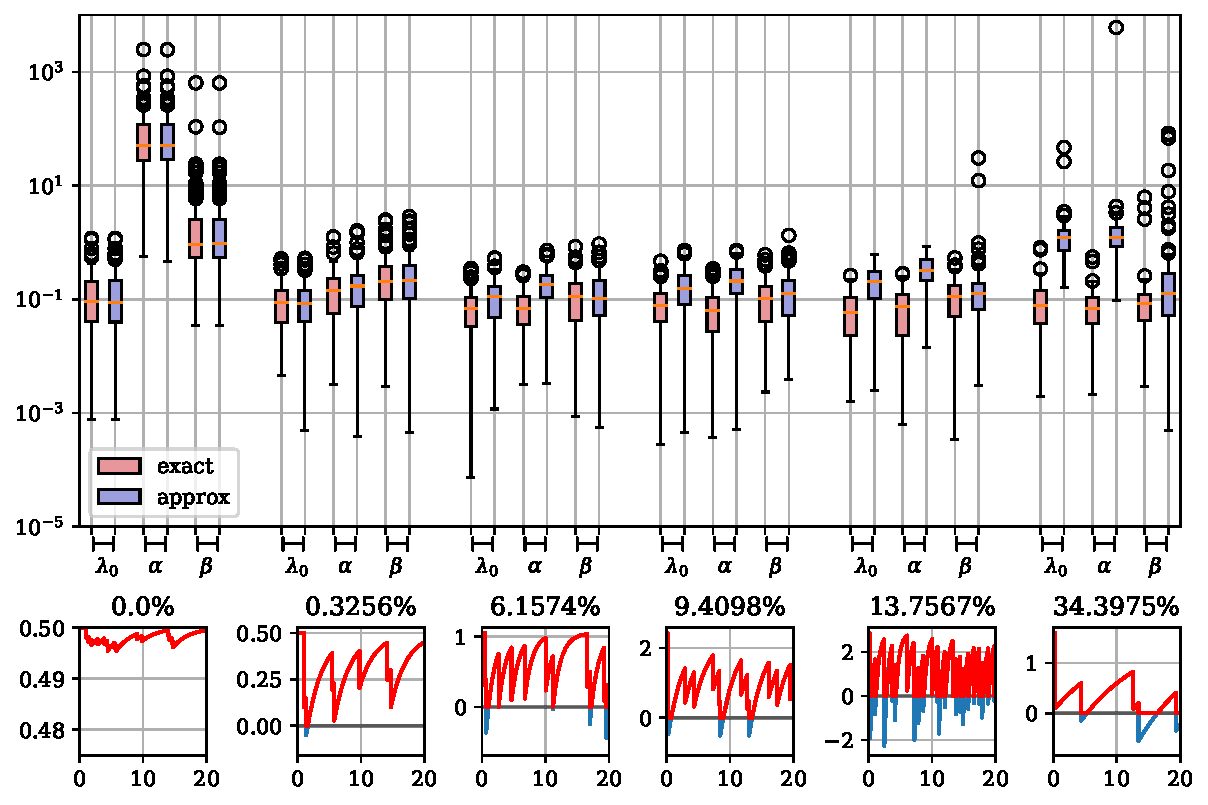
\includegraphics[width=\textwidth]{images/chapter2/intensity_boxplot_log_cropped.pdf}% Remove "cropped" to show all outliers
  \caption{Top panel: relative absolute errors of estimations \(\hat \theta = (\hat \lambda_0, \hat \alpha, \hat \beta)\).
  Bottom panel: example of simulated intensities for each set of values $ \theta = ( \bar \lambda_0,  \bar \alpha,  \bar \beta)$  with the corresponding average percentage of time when the intensities are equal to zero.
  }
  \label{fig:chap1_boxplot_intensity}
\end{figure}

Figure~\ref{fig:chap1_boxplot_intensity} represents the relative absolute errors of estimations \(\hat \theta = (\hat \lambda_0, \hat \alpha, \hat \beta)\) for each of the 6 simulated models.
We observe that the exact approach provides more accurate estimations than the approximated procedure (as illustrated in the boxplots of Figure~\ref{fig:chap1_boxplot_intensity} and by the \(p\)-values of the goodness-of-fit tests in Table~\ref{table:chap1_estim_pvalue}). As expected, the more time the conditional intensity equals 0 (from left to right in Figure~\ref{fig:chap1_boxplot_intensity}), the greater the differences between the two procedures.
Furthermore, the leftmost boxplot confirms that when the underlying intensity is nonnegative both methods are mostly identical.
Let us note that in this case the estimation of \(\bar \alpha\) is rather wrong (the estimation of \(\bar \beta\) is impacted consequently) probably because its value is close to \(0\) compared to the magnitude of \(\bar \lambda_0\).

\begin{table}[!ht]
\centering
\begin{tabular}{cccc|ccc|c}
\hline
    & \multicolumn{3}{c}{Parameters} & \multicolumn{3}{c}{Estimations} & \\
   & $\bar \lambda_0$ &  $\bar \alpha$ &  $\bar \beta$ & $\hat \lambda_0$ &  $\hat \alpha$ &  $\hat \beta$ &  p-value \\
\hline
       Exact&\multirow{2}{*}{0.5 } & \multirow{2}{*}{-0.001 } & \multirow{2}{*}{0.4} &       0.52 & 0.03 & 2.13 & 0.38\\
       Approx&      &       &       & 0.52 & 0.03 & 2.11 & 0.38\\ \hline
       Exact&\multirow{2}{*}{0.5 } & \multirow{2}{*}{-0.2 } & \multirow{2}{*}{0.4 } &       0.51 & -0.21 & 0.45  & 0.42    \\
       Approx&      &       &       &0.51 & -0.22 & 0.47 & 0.42\\ \hline
       Exact&\multirow{2}{*}{1.05 } & \multirow{2}{*}{-0.75 } & \multirow{2}{*}{0.8 } &       1.06 & -0.76 & 0.83 & 0.43  \\
       Approx&      &       &       &1.12 & -0.88 & 0.84 & 0.35\\ \hline
       Exact&\multirow{2}{*}{2.43 } & \multirow{2}{*}{-0.98 } & \multirow{2}{*}{0.4} &       2.59 & -1.00 & 0.38 & 0.53  \\
       Approx&      &       &       & 2.90 & -1.21 & 0.40 & 0.45 \\ \hline
       Exact&\multirow{2}{*}{2.85 } & \multirow{2}{*}{-2.5 } & \multirow{2}{*}{1.8} &       2.81 & -2.56 & 1.87 & 0.36\\
       Approx&      &       &       &$1.55\times10^{4}$ & $-1.63\times10^{7}$ & 3.04  & 0.07\\ \hline
       Exact&\multirow{2}{*}{1.6 } & \multirow{2}{*}{-0.75 } & \multirow{2}{*}{0.1} &       1.62 & -0.76 & 0.11 & 0.42   \\
       Approx&      &       &       &$2.72\times10^{7} $& $-2.31\times10^{10}$  & 0.27  & $2.14\times10^{-05}$\\
\hline
\end{tabular}
\caption{
\change{Quantitative assessment of the numerical study: sets of true parameters (left), average estimations over 50 repetitions (middle) and average \(p\)-values over 50 independent realisations for the test of Section~\ref{sec:chap1_goodness}}.
}
\label{table:chap1_estim_pvalue}
\end{table}

\section{Discussion}

In this paper we proposed a maximum likelihood approach for Hawkes processes that can handle both self-exciting and self-regulating scenarios, the first case being already covered in the literature and the latter being our main contribution. For this purpose, we define the concepts of underlying intensity function and restart times when working with monotone kernel functions. In particular we obtain exact expressions of the compensator for the exponential Hawkes process which is the key step of the estimation procedure.
We present numerical results on synthetic data that show the efficiency of our procedure, with a substantial improvement compared to approximated approaches when the intensity function is frequently null.

From a theoretical point of view, future work will consist in adapting analytical results to study the convergence of our estimator in the self-regulating case. Regarding modeling, it would be of great interest to consider kernel functions outside the classical exponential scenario.
Another important step is the extension of our concepts and algorithms to the multivariate version of the process, which is not straightforward since in the multivariate setting the expression of the restart times are no longer explicit.
This last point is essential in order to target real-world datasets since in many applications, being limited to the univariate case will lead to detect self-excitation. However, a model that accounts for potential inhibition effects is of great interest when considering interactions between events of different natures, which will typically be modeled by a multivariate process. This multidimensional extension is the object of a future work, with a further perspective to use our procedure in neuroscience applications in order to detect attraction and repulsion effects between neurons.

\begin{subappendices}
%\renewcommand\thesection{\thechapter.\Alph{section}}
\section{Proof of Proposition~\ref{prop:chap1_exp}}
\label{app:chap1_appendix}

Let us begin by expressing the underlying intensity function between two event times.
First, \(\lambda^\star(t) = \lambda_0\) for \(t\in[0,T_1)\).
Then, for any $k\in\NN$, for all $t \in [T_k,T_{k+1})$, the underlying intensity is differentiable in \(t\) and
\begin{equation*}
    (\lambda^\star)'(t) = -\beta(\lambda^\star(t) - \lambda_0)\,,
\end{equation*}
with the left condition: $\lambda_k^\star := \lambda^\star(T_k)$.
Solving this differential equation leads to
\begin{equation}\label{eq:chap1_markov_expression}
    \lambda^\star(t) = \lambda_0 + (\lambda_k^\star - \lambda_0)\mathrm{e}^{-\beta(t - T_k)}\,.
\end{equation}

Now, by definition of the restart time $T_k^\star = \inf{\{t\geq T_k\mid \lambda(t) > 0\}}$, we have that if $\lambda_k^\star \geq 0$, then $T_k^\star = T_k$. Otherwise, as $\lambda^\star$ is continuous on the interval $[T_k,T_{k+1})$, we obtain $T_k^\star$ by solving for $t$: \(\lambda^\star(t) = 0\).
Thus, by Equation~\eqref{eq:chap1_markov_expression}:
\begin{align*}
    \lambda^\star(T_k^\star) = 0
    \iff T_k^\star = T_k + \beta^{-1}\log{\left(\frac{\lambda_0 - \lambda^\star_k}{\lambda_0}\right)}\,.
\end{align*}
Gathering both situations, we obtain the first part of Proposition~\ref{prop:chap1_exp}: \[T_k^\star = T_k + \beta^{-1}\log{\left(\frac{\lambda_0 - \lambda^\star_k}{\lambda_0}\right)} \II_{\lambda_k^\star < 0}\].

Let now $k\in\{1,\ldots,N(t)\}$ and $\tau\in[T_{k}^\star,T_{k+1}]$.
By Equation~\eqref{eq:chap1_markov_expression},
\begin{align*}
    \int_{T_{k}^\star}^{\tau}{\lambda^\star(u)\,\mathrm{d}u}
    &= \int_{T_{k}^\star}^{\tau} \left( \lambda_0 + (\lambda_{k}^\star - \lambda_0)\mathrm{e}^{-\beta(u - T_{k})} \right)\,\mathrm{d}u\\
    &= \lambda_0(\tau - T_{k}^\star) + \beta^{-1}(\lambda_{k}^\star - \lambda_0)(\mathrm{e}^{-\beta(T_{k}^\star-T_{k})}-\mathrm{e}^{-\beta(\tau-T_{k})})\,,
\end{align*}
which is the second part of Proposition~\ref{prop:chap1_exp}.

\section{Simulation algorithm}
\label{app:chap1_simulation}

Algorithm~\ref{alg:chap1_simulation} builds upon Ogata's thinning simulation method \parencite[Proposition 1]{Ogata1981} in order to handle Hawkes processes with either self-excitation or inhibition.

\begin{algorithm}[!ht]
\SetAlgoLined
 \textbf{Input} Parameters $\lambda_0$, $h$ a monotone function, and a stopping criteria (end-time $T$ or maximal number of jumps $N_{max}$)\;
 \textbf{\underline{Initialization}} Initialize $\lambda_k =\lambda_0$, $t_k=0$\ and list of times $\mathcal{T} = \emptyset$\;
 \While{\textnormal{Stopping criteria not fulfilled}}{
 Set $\lambda_{max} = \max(\lambda_0,\lambda_k)$\;
 Generate candidate time $t_{cand} = t_k - \frac{\log(U_1)}{\lambda_{max}}$, $U_1\sim U([0,1])$\;
 Estimate intensity $\lambda_k = \lambda(t_{cand})$ using sequence of times $\mathcal{T}$\;
 Sample $U_2\sim U([0,1])$\;
 \If{$U_2 \leq \frac{\lambda_k}{\lambda_{max}}$}{
        Add $t$ to sequence of times $\mathcal{T}$\;
        Update $\lambda_k = \lambda_k + \alpha$\;
     }
 Set $t_k = t_{cand}$\;
 }
 \Return the sequence of jumps $\mathcal{T}$.
 \caption{Thinning algorithm for monotone Hawkes process.}
 \label{alg:chap1_simulation}
\end{algorithm}

\end{subappendices}
\leadchapter{
    The multivariate Hawkes process is a past-dependent point process used to model the relationship of event occurrences between different phenomena.
    Although the Hawkes process was originally introduced to describe excitation interactions, which means that one event increases the chances of another occurring, there has been a growing interest in modelling the opposite effect, known as inhibition.
    In this chapter, we focus on how to infer the parameters of a multidimensional exponential Hawkes process with both excitation and inhibition effects. Our first result is to prove the identifiability of this model under a few sufficient assumptions. Then we propose a maximum likelihood approach to estimate the interaction functions, which is, to the best of our knowledge, the first exact inference procedure in the frequentist framework.
    Our method includes a variable selection step in order to recover the support of interactions and therefore to infer the connectivity graph.
    A benefit of our method is to provide an explicit computation of the log-likelihood, which enables in addition to perform a goodness-of-fit test for assessing the quality of estimations.
    We compare our method to standard approaches, which were developed in the linear framework and are not specifically designed for handling inhibiting effects.
    We show that the proposed estimator performs better on synthetic data than alternative approaches. We also illustrate the application of our procedure to a neuronal activity dataset, which highlights the presence of both exciting and inhibiting effects between neurons.    
}
\chapter[][Inference of multivariate exponential Hawkes processes with inhibition]{Inference of multivariate exponential Hawkes processes with inhibition and application to neuronal activity}\label{chapter:multivariate_inhibition}

% sec, eq, fig, assu, lemma, prop, th, hyp, cor, ex, tab, app, alg

\section{Introduction}

A Hawkes process is a point process in which each point is commonly associated with event occurrences in time. In this past-dependent model, every event time impacts the probability that other events take place subsequently. These processes are characterised by the conditional intensity function, seen as an instantaneous measure of the probability of event occurrences. Since their introduction in \textcite{Hawkes1971}, Hawkes processes have been applied in a wide variety of fields, for instance in seismology \parencite{Ogata1988}, social media \parencite{Rizoiu2017}, criminology \parencite{Olinde2020} and neuroscience \parencite{Lambert2018}.

The multidimensional version of this model, referred to as the multivariate Hawkes process, describes the appearance of different types of events, the occurrences of which are influenced by all past events of all types. Each interaction between two types of events is encoded in kernel functions, also called interaction functions.
Originally this model takes only into account mutually exciting interactions - an event increases the chances of others occurring -
by assuming that all kernel functions are non-negative.
A specificity of self-exciting Hawkes processes is their branching structure, also known as cluster structure.
Introduced in \textcite{Hawkes1974}, this parallel between Hawkes processes and branching theory has provided the first theoretical background for the self-exciting Hawkes model, in particular existence and expected number of points on a finite interval.
Estimation methods in the literature are vast including maximum likelihood estimators \parencite{Ozaki1979,Guo2018} and method of moments \parencite{DaFonseca2013}. 
Nonparametric approaches include an EM procedure introduced in \textcite{Lewis2011}, estimations obtained via the solution of Wiener-Hopf equations \parencite{Bacry2016} or by approximating the process through autoregressive models \parencite{Kirchner2017} or through functions in reproducing kernel Hilbert spaces \parencite{Yang2017}.

Although the self-exciting Hawkes process remains widely studied, there has been a growing interest in modeling the opposite effect, known as inhibition, in which the probability of observing an event is lowered by the occurrence of certain events. In practice, this amounts to considering negative kernel functions. In order to maintain the positivity of the intensity function, a non-linear operator is added to the expression which in turns entails the loss of the cluster representation. This model known as the non-linear Hawkes process was first presented in \textcite{Bremaud1996}, where existence of such processes was proved via construction using bi-dimensional marked Poisson processes. Such approach of analysis has been used in the literature as in \textcite{Chen2017}, where a coupling process is established and leveraged to obtain theoretical guarantees on cross-analysis covariance. Another approach is presented in \textcite{Costa2020}, where renewal theory allows to obtain limit theorems for processes with bounded support kernel functions. Estimation methods focus mainly on nonparametric methods for general interactions and non-linear functions, as found in \textcite{Bacry2016,Sulem2024}.

In the last years,
alternative models have been designed in order to take into account inhibiting effects in Hawkes processes.
An example is the neural Hawkes process, presented in \textcite{Mei2017,Zuo2021}, which combines a multivariate Hawkes process and a recurrent neural network architecture.
In \textcite{Duval2021}, a multiplicative model considers two sets of neuronal populations, one exciting and another inhibiting, and each intensity function is the product of two non-linear functions (one for each group).
Another model is presented in \textcite{Olinde2020} and called self-limiting Hawkes process.
It includes the inhibition as a multiplicative term in front of a the traditional self-exciting intensity function. 

In this chapter, we present a maximum likelihood estimation method for multivariate Hawkes processes with exponential kernel functions, that works for both exciting and inhibiting interactions, as modelled by \textcite{Bremaud1996, Chen2017}.
This work builds upon the methodology for the univariate case, presented in \textcite{bonnet2021}, by focusing in the intervals where the intensity function is positive.
We show that, under a weak assumption on the kernel functions, these intervals can be determined exactly.
We can then write for each dimension the integral of the intensity function, known in the literature as the compensator, which in turn provides an explicit expression of the log-likelihood.
This enables to build the corresponding maximum likelihood estimator and we complete our procedure with a variable selection step to recover the significant interactions within the whole process. This is of particular interest since it provides a graphical interpretation of the model and it can also be used a reduction dimension tool.
Our numerical procedure is implemented
in Python and freely available on GitHub.\footnote{\url{https://github.com/migmtz/multivariate-hawkes-inhibition}}
As a by-product of our method, the closed-form expression of the compensator also allows to assess goodness-of-fit via the Time Change Theorem and multiple testing.
We carry out a numerical study on simulated data and on a neuronal activity dataset \parencite{Petersen2016,Radosevic2019}.
The performance of our approach is compared to estimations obtained via approximations from \textcite{Bacry2020} and \textcite{Lemonnier2014}, and we show that our method not only achieves better estimations but is capable of identifying correctly the interaction network of the process.

To outline this chapter, Section~\ref{sec:chap3_presentation} presents the multivariate Hawkes process framework and reviews the literature regarding inference of non-linear Hawkes processes.
In Section~\ref{sec:chap3_exponential}, we detail our procedure, including the maximum likelihood estimation, variable selection and goodness-of-fit test to assess the quality of the estimations. We also address the question of identifiability of the model, that we prove under a few sufficient conditions. 
The whole procedure is illustrated on simulated data in Section~\ref{sec:chap3_numerical} and applied to a neuronal activity dataset in Section~\ref{sec:chap3_neuron}. In Section \ref{sec:chap3_discussion} we discuss our contributions and its current limitations along with interesting perspectives for future work.

\section{The multivariate Hawkes process}\label{sec:chap3_presentation}
    \subsection{Definition}
    A multivariate Hawkes process $N = (N^1, N^2, \ldots, N^d)$ of dimension $d$ is defined by $d$ point processes on $\RR_+^*$, denoted $N^i\colon \mathcal B(\RR_+^*) \to \NN$, where $\mathcal{B}(\RR_+^*)$ is the Borel algebra on the set of positive numbers.

    Each process $N^i$ can be characterised by its associated event times $\left(T_k^i\right)_k$ and its conditional intensity function, defined for all \(t \ge 0\) by
    \begin{align}
    \lambda^i(t) &= \adaptedpar{\mu_i + \sum_{j=1}^{d}{\int_{0}^{t}{h_{ij}(t-s)\,\mathrm{d}N^j(s)}}}^+\nonumber\\ &= \adaptedpar{\mu_i + \sum_{j=1}^{d}\sum_{T_k^j \leq t}{h_{ij}(t-T^j_k)}}^+\label{eq:chap3_dimensional_c_intensity}\,,
    \end{align}
    where
    $x^+ = \max{(0,x)}$.
    Here, the quantity $\mu_i\in\RR_+^*$ is called the baseline intensity and each interaction or kernel function $h_{ij}\colon \RR_+^* \to \RR$ represents the influence of the process $N^j$ on the process $N^i$ and $T^j_k$ corresponds to the $k$-th event time of process $N^j$.

    \begin{remark}
      The positive-part function in Equation~\eqref{eq:chap3_dimensional_c_intensity} is needed to ensure the non-negativity of \(\lambda^i\) in the presence of strong inhibiting effects, that is when some interaction functions \(h_{ij}\) are sufficiently negative compared to positive contributions.
      Concretely, the positive part does not affect the intensity function if inhibiting effects are in minority compared to the positive contributions (exciting effects or baseline intensities).
    \end{remark}
    \begin{remark}
        Equation~\eqref{eq:chap3_dimensional_c_intensity} may question the reader for two reasons.
        First, it is the cadlag definition of a the conditional intensity of a Hawkes process.
        It's our choice to prefer it to the caglad version but all the results presented here can be written in this setting.
        Second, it is considered that the history is empty for \(t < 0\).
        It is a common choice for statistical inference (a finite amount a times is observed) while the infinite history is preferred for a probabilistic analysis based on a stationary assumption.
    \end{remark}
    
    
    For each process \(N^i\) and for all $t\geq 0$, let us note $N^i(t) = \sum_{k\geq 1}{\II_{T_k^i \leq t}}$ the measure of \((0, t]\) and the compensator \[\Lambda^i(t) = \int_{0}^{t}{\lambda^i(u)\,\mathrm{d}u}\,.\]

    The process $N$ can be seen as a point process on $\RR_+^*$, where for any $B\in\mathcal{B}(\RR^*_+)$, $N(B) = \sum_{i=1}^{d}{N^i(B)}$.
    Similarly to a univariate process, \(N\) can be characterised by its conditional intensity \(\lambda\) (also called total intensity):
    \begin{equation}\label{eq:chap3_total_intensity}
        \lambda(t) = \sum_{i=1}^{d}{\lambda^i(t)}\,,
    \end{equation}
    and by its compensator
    \[\Lambda(t)=\int_{0}^{t}{\lambda(u)\,\mathrm{d}u} =\sum_{i=1}^{d}{\Lambda^i(t)}\,.\]

    From this point of view, the process \(N\) is associated to event times $\left(T\park\right)_k = \left(T_{u_k}^{m_k}\right)_k$, corresponding to the ordered sequence composed of $\bigcup_{i=1}^{d}\{T_k^i \mid k>0\}$,
    and we may define, for every \(t\ge 0\), $N(t) = \sum_{k\geq 1}{\II_{T\park \leq t}} = \sum_{i=1}^{d}{N^i(t)}$.
    Here, $(u_k)_k$ is the random ordering sequence and $(m_k)_k$ the sequence of marks that make it possible to identify to which dimension each time corresponds.
    These marks can be written as \[m_k = \sum_{j=1}^{d}{j\II_{N^j\left(\{T\park\}\right) = 1}}\,.\]
    
    \begin{remark}
    A more detailed introduction of multivariate point processes via the concept of marked point processes can be found in \textcite[Chapter 6.4]{DaleyV1}
    \end{remark}

    As the aim of this chapter is to describe a practical methodology for estimating the conditional intensities \(\lambda_1\), \dots, \(\lambda_d\) via maximising the log-likelihood, the latter quantity has to be made explicit.
    Let \(t \ge 0\) and assume that event times
    $\left\{ T_k^i : 1 \le k \le N_i(t), 1 \le i \le d \right\}$
    are observed in the interval \((0, t]\).
    Then, given a parametric model $\mathcal{P} = \{(\lambda_{\theta_1}^1, \dots, \lambda_{\theta_d}^d)\colon \theta = (\theta_1, \dots, \theta_d) \in \Theta_1 \times \dots \times \Theta_d\}$ (and associated compensators \(\Lambda_{\theta_1}^1, \dots, \Lambda_{\theta_d}^d\)) for conditional intensity functions \(\lambda^1, \dots, \lambda^d\), for every \(\theta \in \Theta\), the log-likelihood $\ell_t(\theta)$ reads \textcite[Proposition 7.3.III.]{DaleyV1}
    \begin{equation*}
      \ell_t(\theta) = \sum_{i=1}^{d}{\ell_t^i(\theta_i)}\,,\nonumber 
    \end{equation*}
    with
    \begin{equation}\label{eq:chap3_general_log_likelihood}
      \ell_t^{i}(\theta_i) = \sum_{k=1}^{N^i(t)}{\log{\lambda^i_{\theta_i}(T_k^{i-})}} - \Lambda_{\theta_i}^i(t)\,,
    \end{equation}
    where $\lambda^i_{\theta_i}(T_k^{i-}) = \lim_{t\to T_k^{i-}}{\lambda_{\theta_i}^i(t)}$ and with convention $\log{(x)} = -\infty$ for $x\leq 0$.

    The heart of the problem in deriving a maximum likelihood estimator for the conditional intensities \(\lambda^i\) is being able to evaluate exactly the compensator values \(\Lambda_\theta^i(t)\) for every possible \(\theta \in \Theta\), which requires to determine when the conditional intensities \(\lambda^i\) are non-zero.
    The forthcoming sections clear this point up.


  \subsection{Related work}\label{sec:chap3_literature}
    Estimation methods for Hawkes processes have focused mainly on self-exciting interactions (by assuming $h_{ij} \geq 0$). In \textcite{Ozaki1979}, the author presents the maximum likelihood estimation method for univariate processes with exponential kernel \(h(t) = \alpha \mathrm{e}^{-\beta t}\) (\(\alpha>0\), \(\beta>0\)), the same method being established in \textcite{Mishra2016} for the power law kernel function \(h(t) = \frac{\alpha\beta} {(1 + \beta t)^{1 + \gamma}}\) (\(\alpha>0\), \(\beta>0\), \(\gamma > 0\)). In \textcite{Chen2018} the maximum likelihood method is presented for the multivariate version with exponential kernel, while \textcite{Bacry2020} proposed an inference method based on optimising a least-squares criterion. Other methods in the parametric setting include spectral analysis \parencite{Adamopoulos1976}, EM algorithm \parencite{Veen2008} and method of moments \parencite{DaFonseca2013}.

    Estimators of the interaction functions \(h_{ij}\) are also presented in a nonparametric setting. For instance, \textcite{Yang2017} proposed to estimate \(h_{ij}\) in a reproducing kernel Hilbert space.
    \textcite{Reynaud2014} proposed a decomposition of the interaction functions \(h_{ij}\) on a histogram basis with bounded support, the estimation of which are obtained by minimising a least-squares contrast.
    Hawkes processes with excitation have also been studied in a Bayesian context, with likelihood-based approaches, as in \textcite{Rasmussen2013} for the univariate case and in \textcite{Donnet2020} for multivariate processes.

    Although inhibiting effects in Hawkes processes were first mentioned in \textcite{Bremaud1996}, they have only met a growing interest in the last decade.
    Concerning inference, most of the known methods are not designed for handling the inhibiting case: nevertheless some are able in practice to estimate negative interactions by minimising a least-squares criterion, but without guaranteeing that the estimated intensity functions remain non-negative \parencite{Reynaud2014, Bacry2020}.
    A similar approach is proposed in \textcite{Lemonnier2014} for maximum likelihood estimation, where the compensator \(\Lambda^i\) is approximated by integrating
    the conditional intensity $\lambda^i$ without the positive part function (see Equation~\eqref{eq:chap3_dimensional_c_intensity}).
    Obviously, these methods should perform well when the intensities remain mostly positive, but it is unclear how they will adapt to scenarios when the intensities are frequently equal to zero due to inhibiting terms.
    A similar remark is mentioned in \textcite{Bacry2016} concerning their estimation method, that can provide negative estimations of the interactions only if there is a negligible chance of the intensities to be null.
    
    Inference procedures that are specifically dedicated to Hawkes processes with inhibition are scarcer in the literature. \textcite{Sulem2024} presents various results for non-linear Hawkes processes including inhibition effects: existence, stability and Bayesian estimation for kernel functions with bounded support.
    \textcite{Deutsch2022} presents choices of priors for Bayesian estimation based on a new reparametrisation of the process.

    Lastly, \textcite{bonnet2021} presents a maximum likelihood estimation adapted to the univariate Hawkes process with inhibition and monotone kernel functions.
    The decisive contribution of this work is to give, for an exponential kernel \(h(t) = \alpha \mathrm{e}^{-\beta t}\) (\(\alpha \in \RR\), \(\beta>0\)), a closed-form expression of restart times, which are defined as the instants at which the single conditional intensity becomes non-zero.
    This makes possible to compute explicitly the compensator and then the log-likelihood.
    Yet, this study is limited to the univariate case.

    This work goes a step forward in estimation of multivariate Hawkes processes with inhibition, by providing the first exact maximum likelihood method for exponential interactions $h_{ij}(t) = \alpha_{ij}\mathrm{e}^{-\beta_{ij}t}$, combined with a variable selection procedure. As it will be explained in the next section, the proposed approach also enables to perform standard goodness-of-fit tests. It has to be noted that the concurrent work of \textcite{Deutsch2022} proposed a similar approach for multivariate Hawkes processes to exactly compute the compensator,
    but was used neither for maximum likelihood estimation, nor for goodness-of-fit tests.


    \section{Estimation and goodness-of-fit}\label{sec:chap3_exponential}

    \subsection{Introductive example}
    Before motivating and explaining the estimation procedure proposed in this chapter, we present an example of multivariate Hawkes process.
    Figure~\ref{fig:chap3_2_dimension_example} depicts in red conditional intensities \(\lambda^1\) and \(\lambda^2\) for a realisation of a \(2\)-dimensional Hawkes process (see the forthcoming section for the definition of underlying intensities). The existence of such a process (along with its stationarity) is ensured by controlling the spectral radius $\rho(S^+) < 1$ of the matrix $S^+ = (\|h_{ij}^+\|_1)_{ij}$ \parencite{Deutsch2022}. Similar results with slightly different conditions can be found in \textcite{Bremaud1996} and \textcite{Sulem2024}.
    The simulation has been carried out with baselines \(\mu_1 = 0.5\) and \(\mu_2 = 1.0\),
    and with exponential kernels \(h_{ij}(t) = \alpha_{ij} \mathrm{e}^{-\beta_{ij}t}\) parameterised by:
    \[
      \begin{pmatrix}
      \alpha_{11} & \alpha_{12}\\
      \alpha_{21} & \alpha_{22}
      \end{pmatrix}=
      \begin{pmatrix}
      -1.9 & 3.0\\
      0.9 & -0.7
      \end{pmatrix},
      \qquad
      \text{and}
      \qquad
      \begin{pmatrix}
      \beta_{11} & \beta_{12}\\
      \beta_{21} & \beta_{22}
      \end{pmatrix} =
      \begin{pmatrix}
      2.0 & 20.0\\
      3.0 & 2.0
      \end{pmatrix}\,.
    \]
    These kernels have been chosen such that both processes are self-inhibiting ($\alpha_{11}, \alpha_{22} < 0$) but inter-exciting ($\alpha_{12}, \alpha_{21} > 0$).

    \begin{figure*}[!ht]
    \centering
    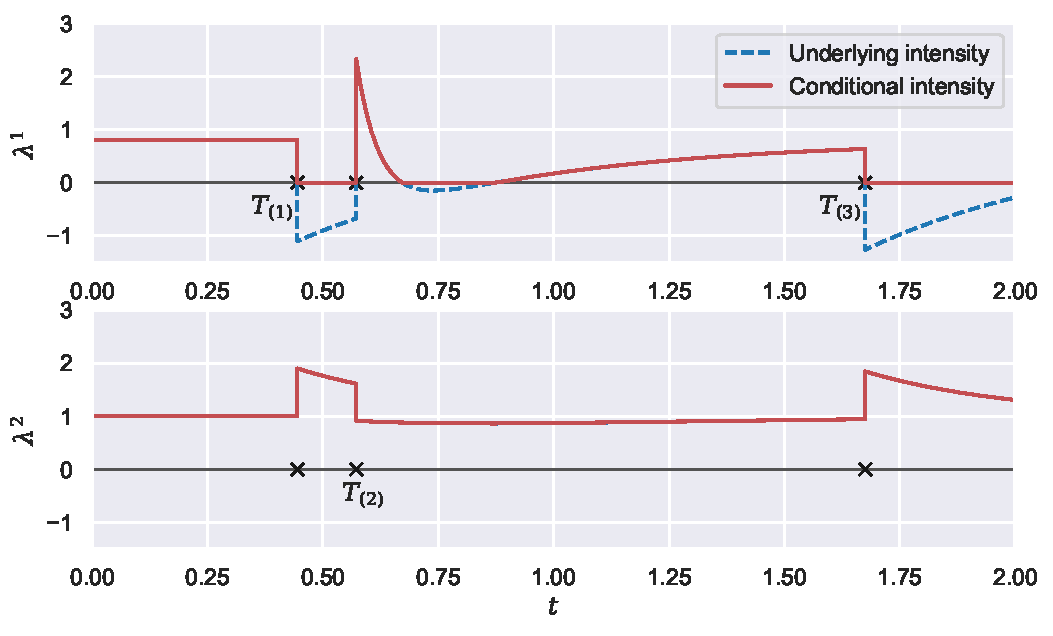
\includegraphics[width=.75\linewidth]{images/chapter3/timesMarkedMulti.pdf}
    \caption{Simulation of a \(2\)-dimensional Hawkes process. Each cross corresponds to an event time, and each $T\park$ is shown in its corresponding process.}
    \label{fig:chap3_2_dimension_example}
    \end{figure*}

    The goal of this work is to establish a parametric estimation method, via maximum likelihood estimation, that is able to handle both excitation and inhibition frameworks in the multivariate case.
    For this purpose, it is necessary to compute explicitly the log-likelihood \(\ell_t(\theta)\) (see Equation~\eqref{eq:chap3_general_log_likelihood}) and in particular to evaluate the compensator \(\Lambda_\theta^i\), expressed as an integral of \(\lambda_\theta^i\).
    For the latter, the main challenge is to determine when conditional intensities \(\lambda^i\) are non-zero, that is on which intervals they are tailored by the exponential interaction functions and not by the positive-part operator.

    In \textcite{bonnet2021}, the authors solved this challenge for univariate processes by remarking that the conditional intensity is monotone between two event times.
    Figure~\ref{fig:chap3_2_dimension_example} illustrates that this is not necessarily true for multivariate processes (here, between \(T_{(2)}\) and \(T_{(3)}\)).
    This constitutes the major difficulty we have to cope with.

  \subsection{Underlying intensity and restart times in the multivariate setting}

    From now on, let us focus on the exponential model \parencite{Hawkes1971}, where each interaction function $h_{ij}$ is then defined as
    \[h_{ij}(t) = \alpha_{ij}\mathrm{e}^{-\beta_{ij}t}\,,\]
    with $\alpha_{ij}\in\RR$ and $\beta_{ij}\in\RR_+^*$ for $i,j\in \{1,\ldots, d\}$.
    For each $i\in\{1,\ldots, d\}$, the underlying intensity function $\lambda^{i\star}$ is defined as in \textcite{bonnet2021} for the univariate case:
    \[\lambda^{i\star}(t) = \mu_i + \sum_{j=1}^{d}{\int_{0}^{t}{h_{ij}(t-s)\,\mathrm{d}N^j(s)}}\,.\]
    This quantity coincides with the conditional intensity \(\lambda^i\) when it is non-zero, and is non-positive otherwise.
    In particular, we can observe that \(\lambda^i (t) = \left( \lambda^{i\star}(t) \right)^+\) (see Figure~\ref{fig:chap3_2_dimension_example}).

    As explained in the previous section, the main difficulty of the multivariate exponential setting is the non-monotony of conditional intensities \(\lambda^i\) between two event times.
    Determining intervals where \(\lambda^i\) is non-zero (that is when \(\lambda^{i\star}\) is positive) would require to numerically find the roots of a high-degree polynomial, which is expensive and inexact.
    To alleviate this problem, we introduce Assumption~\ref{assu:chap3_beta}.

    \begin{assumption}\label{assu:chap3_beta}
    For each $i\in\{1,\ldots, d\}$, there exists $\beta_i\in\RR_+^*$ such that $\beta_{ij} = \beta_i$ for all $j\in\{1,\ldots, d\}$.
    \end{assumption}

    \begin{remark} This model with constant recovery rates $\beta_i$ has been studied before in the works of \textcite{Ogata1981} in the self-exciting version of a 2-dimensional Hawkes process. Intuitively, this assumption considers the situation where the rate of ``dissipation'' of any internal or external effect is dependent only on the receiving phenomenon. For instance, for neuronal interactions, each activation from neuron $j$ will have an impact on a connected neuron $i$ dependent on both neurons $(\alpha_{ij})_{ij}$ but the ``recovery'' time can be assumed to depend only on the connected neuron $i$ \((\beta_{i})_i\).
    \end{remark}

    As we will see in Lemma~\ref{lemma:chap3_restart_times}, this assumption enables to recover the monotony of the conditional intensities between two times.
    It remains now to determine when the underlying intensity \(\lambda^{i\star}\) is negative.
    To do so, we define the restart times in the multivariate framework, to be,
    for any \(k\) and \(i\):
    \[T\park^{i\star} = \min\adaptedpar{\inf{\{t\geq T\park \colon \lambda^{i\star}(t) \geq 0\}}, T\park[k+1]}.\]
    
    {\begin{figure*}[!ht]
    \centering
    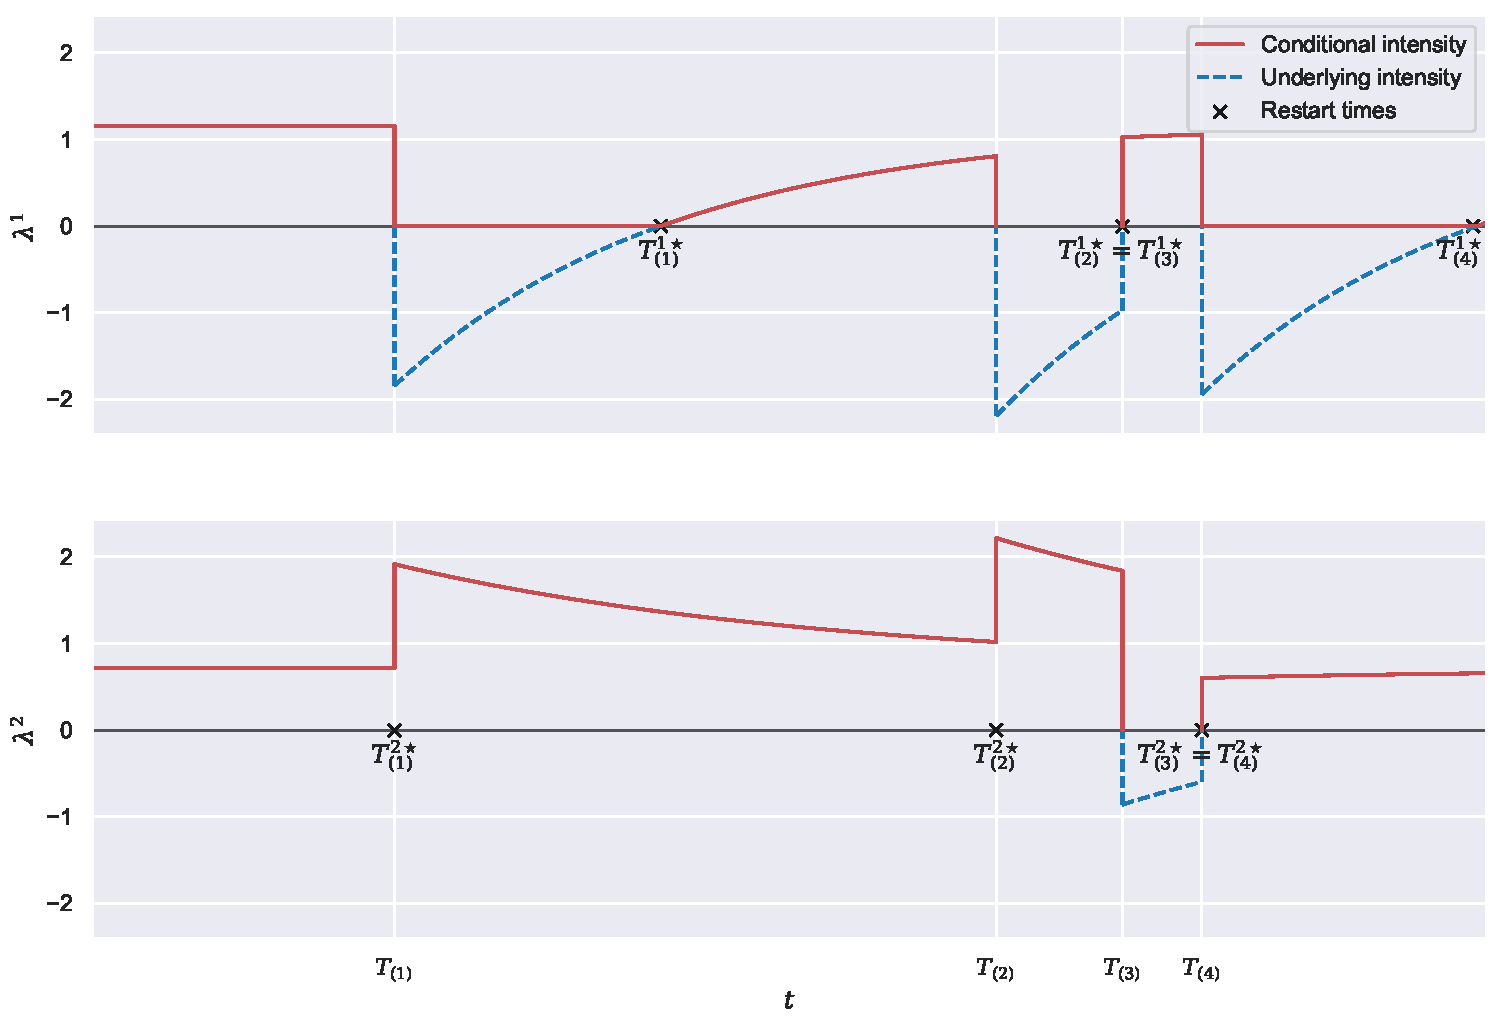
\includegraphics[width=0.8\linewidth]{images/chapter3/restarTimesMarkedMulti.pdf}
    \caption{Illustration of restart times $(T\park^{\star})_{1\leq k \leq 4}$ for each subprocess of a 2-dimensional process associated with event times $(T\park[k])_{1\leq k \leq 4}$.}
    \label{fig:chap3_restarttimes}
    \end{figure*}}
    
     As exemplified in Figure~\ref{fig:chap3_restarttimes}, the restart time $T\park^{i\star}$ (associated to the sub-process $i$) corresponds to the first instant between $T\park$ and $T\park[k+1]$ from which $\lambda^{i\star}(t)$ becomes non-negative (or $T\park[k+1]$ if this instant does not exist).
    Intuitively, it means that $\lambda^{i}(t) = \lambda^{i\star}(t)$ on $(T\park^{i\star}, T\park[k+1])$ and $\lambda^{i}(t) = 0$ elsewhere on  $(T\park$, $T\park[k+1])$.
    This is formalised in Lemma~\ref{lemma:chap3_restart_times}.
    In particular, it appears that the restart time $T\park^{i\star}$ can be expressed as a function of $$T\park + \beta_i^{-1}\log{\adaptedpar{\frac{\mu_i - \lambda^{i\star}(T\park)}{\mu_i}}}\,,$$
      which is the single root to the equation $\mu_i + (\lambda^{i\star}(T\park) - \mu_i)\mathrm{e}^{-\beta_i(t-T\park)} = 0$ on the interval $[T\park, +\infty)$ when $\lambda^{i\star}(T\park) < 0$ (see top panel of Figure~\ref{fig:chap3_restarttimes}).
      Then, Proposition~\ref{prop:chap3_compensator} gives an explicit formulation of the compensator of each subprocessi \(N^i\), which is needed to compute the log-likelihood (see Equation~\eqref{eq:chap3_general_log_likelihood}).
      The proofs of these two results are presented respectively in Appendix~\ref{app:chap3_proof_lemma} and Appendix~\ref{app:chap3_proof_prop_compensator}.

    \begin{lemma}\label{lemma:chap3_restart_times}
    If Assumption~\ref{assu:chap3_beta} is granted, then for each $i\in\{1,\ldots, d\}$ and any $k\geq1$: 

    \begin{equation}\label{eq:chap3_restart_times_exponential}
        T\park^{i\star} = \min{\adaptedpar{t^\star_k, T\park[k+1]}}\,.
    \end{equation}
    where
    \[t^\star_k = \adaptedpar{T\park + \beta_i^{-1}\log{\adaptedpar{\frac{\mu_i - \lambda^{i\star}(T\park)}{\mu_i}}}\II_{\{\lambda^{i\star}(T\park) < 0\}}}\]

    Furthermore,
    for all \(t \in (T\park, T\park[k+1])\),
    \[
      \lambda^i(t) =
      \begin{cases}
        \lambda^{i\star}(t) > 0 & \text{if } t \in (T\park^{i\star}, T\park[k+1])\\
        0 & \text{otherwise}.
      \end{cases}
    \]
    \end{lemma}

    \begin{proposition}\label{prop:chap3_compensator}[Compensator for multivariate exponential kernels]
    Let us suppose that Assumption~\ref{assu:chap3_beta} is granted. For each $i\in\{1,\ldots, d\}$ the compensator $\Lambda^i$ of the process $N^i$ reads, $\forall t\geq 0$:
    \begin{equation}\label{eq:chap3_compensator_exponential}
      \Lambda^i(t) =
      \begin{cases}
        \mu_i t & \text{if } t < T\park[1] \\
        \mu_i T\park[1] + \sum_{k=1}^{N(t)} J_k & \text{if } t \geq T\park[1] \,,
      \end{cases}
    \end{equation}
    where for all integer \(k \in \{1, \dots, N(t)\}\):
    \begin{equation*}
      J_k =
      \mu_i \left[\min(t, T\park[k+1] ) - T\park^{i\star}\right] + \beta_i^{-1} \left(\lambda^{i\star}(T\park) - \mu_i \right)
      \left[ \mathrm{e}^{-\beta_i(T\park^{i\star} - T\park)} - \mathrm{e}^{-\beta_i(\min(t, T\park[k+1])- T\park)} \right]\,.
    \end{equation*}
    \end{proposition}
    
  \subsection{Identifiability and likelihood computation}\label{sec:chap3_likelihood}
    As already mentioned in Section~\ref{sec:chap3_presentation}, let \(t \ge 0\) and assume that event times
    $\left\{ T_k^i : 1 \le k \le N_i(t),\right.$ $\left. 1 \le i \le d \right\}$ are observed in the interval \((0, t]\).
    We consider the parametric exponential model for a multivariate Hawkes process of dimension $d$, defined by
    \[
      \mathcal P = \left\{(\lambda^1, \dots, \lambda^d)\colon \lambda^1 \in \mathcal P^1, \dots, \lambda^d \in \mathcal P^d \right\} \,,
    \]
    where for each \(i \in \{1, \dots, d\}\), \(\mathcal P^i\) is the exponential parametric model for the process \(N^i\):
\[
      \mathcal{P}^i
      = \left\{	\lambda_{\theta_i}^i = \left(\mu_i + \sum_{j=1}^{d}{\int_{-\infty}^{t}{\alpha_{ij} \mathrm{e}^{-\beta_i(t-s)}\,\mathrm{d}N^j(s)}}\right)^+ \colon \theta_i = (\mu_i, \alpha_{i1}, \ldots, \alpha_{id}, \beta_i) \in\Theta \,\right\}\,,
    \]
    where $\Theta = \RR_+^\star\times\RR^d\times\RR_+^\star$.
    For a candidate set of intensities \((\lambda_{\theta_1}^1, \dots, \lambda_{\theta_d}^d)\), the underlying intensity functions are denoted \(\lambda_{\theta_i}^{i\star}\) (\(i \in \{1, \dots, d\}\)), the compensators $\Lambda_{\theta_i}^i$
    and the restart times
    $(T^{i\star}_{\theta_i, (k)})_{k}$.
    Now, given a realisation $\left(T\park \right)_{k>0}$ of a multivariate exponential Hawkes process,
    Theorem~\ref{th:chap3_identifiability} establishes the correspondence between the conditional intensities and the parameters.
        
\begin{theorem}[Identifiability]\label{th:chap3_identifiability}
    Let $N=(N^1, \ldots, N^d)$ be a multivariate Hawkes process defined by a set of intensity functions $(\lambda^1_{\theta_1}, \dots, \lambda^d_{\theta_d}) \in \mathcal P$, for some $\theta = (\theta_1, \dots, \theta_d) \in \Theta^d$.
    Let also $\left(T\park \right)_{k>0}$ be a realisation of $N$ and $\mathcal{F}_t$ be the corresponding filtration.
    
    Let us assume that a.s. for every $(i, j) \in \{1, \dots, d\}^2$, $i\neq j$,
    there exist an event time \(\tau\) from process \(N^j\),
    and an event time \(\tau_+ > \tau\) from process \(N^i\), such that:
    \begin{enumerate}
        \item \label{hyp:chap3_ii} $\lambda_{\theta_i}^i(\tau^-) > 0$;
        \item \label{hyp:chap3_iii} there are only events of process $N^j$ in the interval $[\tau, \tau_+)$.
    \end{enumerate} 
    
    Then, for any $\theta' \in \Theta^d$,
    \[
      \forall i \in \{1, \dots, d\},~
      \lambda_{\theta_i}^i(t ~|~ \mathcal{F}_t) = \lambda_{\theta_i'}^i(t ~| \mathcal{F}_t) \text{ a.e.}
      \qquad
      \iff
      \qquad
      \theta = \theta' \,.
    \]
\end{theorem}

The proof is presented in Appendix \ref{app:chap3_proof}. To the best of our knowledge, the only identifiability result for non-linear multivariate Hawkes processes is given by \textcite{Sulem2024} but only if interaction functions $h_{ij}$ have a bounded support. Their proof strongly relies on this assumption since they extend to the multivariate case the renewal properties proved by \textcite{Costa2020} for non-linear univariate Hawkes processes with a bounded kernel.
Their proof also requires some assumptions to ensure that one process is not totally inhibited, which is also a consequence of the assumptions that we propose, as discussed in Section~\ref{sec:chap3_identifiability}. 

    As expected, Proposition~\ref{prop:chap3_compensator} makes it possible to compute explicitly the log-likelihood expressed in Equation~\eqref{eq:chap3_general_log_likelihood} for multivariate exponential Hawkes processes.
    This is formalised in Corollary~\ref{cor:chap3_mle} (and proved in Appendix~\ref{app:chap3_proof_cor_mle}).

    \begin{corollary}\label{cor:chap3_mle}
        Let \(i \in \{1, \dots, d\}\) and \(k\geq 2\) an integer.
        Let us denote
        \[
          S_k^i := T\park[N(T_k^i)-1]
          = T\park[\max\{\ell \in \mathbb N^* : {T\park[\ell]} < T_k^i\}] \,,
        \]
        the time preceding directly \(T_k^i\), the \(k^{\text{th}}\) observation of process \(N^i\).
        
        Then, for all \(\theta \in \Theta\),
        the log-likelihood of process \(N^i\) reads:
        \begin{align}\label{eq:chap3_log_likelihood}
            \ell^i_t(\theta_i) = &\log{\mu_i} + \sum_{k=2}^{N^i(t)}{\log{\adaptedpar{\mu_i + (\lambda^{i\star}_{\theta_i}(S_k^i) - \mu_i)\mathrm{e}^{-\beta_i(T_k^i - S_k^i)}}}} - \Lambda^i_{\theta_i}(t)\,,
        \end{align} where $\Lambda^i_{\theta_i}$ is given by Equation~\eqref{eq:chap3_compensator_exponential} and with convention $\log{(x)} = -\infty$ for $x\leq 0$.

    \end{corollary}

    Algorithm~\ref{alg:chap3_likelihood} in Appendix~\ref{app:chap3_log-lik} presents the iterative computation of the likelihood using Equation~\eqref{eq:chap3_log_likelihood}. In particular, the complexity of the computation is $O(N(t)\times d)$.
    It is then possible to establish the Maximum Likelihood Estimator, which we will refer to as (MLE). These estimators will be denoted by a tilde: $(\tilde\mu_i)_i$, $(\tilde\alpha_{ij})_{ij}$, $(\tilde\beta_i)_i$ and $(\tilde h_{ij})_{ij}$.

\subsection{On identifiability conditions}\label{sec:chap3_identifiability}

        In the previous section we presented a result on the identifiability of multivariate Hawkes process with inhibition via Theorem~\ref{th:chap3_identifiability}.
        Let us mention that identifiability of parameters \(\mu_i\) and \(\beta_i\) do not require any assumption.
	  The challenge of the proof lies in identifying parameters \(\alpha_{ij}\), which is achieved thanks to Conditions~\ref{hyp:chap3_ii} and \ref{hyp:chap3_iii} of Theorem~\ref{th:chap3_identifiability}.
	  Condition~\ref{hyp:chap3_ii} allows to control strong inhibition scenarios by ensuring that each subprocess' intensity is positive sufficiently often, and not only at its own event times,
	  while Condition~\ref{hyp:chap3_iii} enables to disentangle the contributions of each subprocess.
	  We believe that these assumptions are only sufficient and could be weakened at the cost of a more intricate analysis.

    In this section we will discuss this set of conditions by providing two examples of parameters $\alpha_{ij}$ that allow to apply this result along with one counter-example.

\subsubsection{Examples for which the conditions are fulfilled}
    Let us begin with an example of a two-dimensional process.
    In this situation, as soon as both processes have an infinite amount of events,
    Conditions~\ref{hyp:chap3_ii} and \ref{hyp:chap3_iii} boil down to finding indexes \(k\ge1\) and \(k'\ge1\) such that \(\lambda^1({T_k^2}^-)>0\) and \(\lambda^2({T_{k'}^1}^-)>0\).
    Indeed, it is then enough to consider \((\tau, \tau_+) = (T_k^2, T_{N(T_k^2)+1}^1)\) for \((i, j)=(1, 2)\) and \((\tau, \tau_+) = (T_{k'}^1, T_{N(T_{k'}^1)+1}^2)\) for \((i, j)=(2, 1)\).

    \begin{example}\label{ex:chap3_2dim_identifiability}
        Let us assume that $N$ is a two-dimensional Hawkes process with the following matrix for parameters $\alpha_{ij}$:
        \[\begin{pmatrix}
                      \alpha_{11} & \alpha_{12}\\
                      \alpha_{21} & \alpha_{22}
                      \end{pmatrix}=
                      \begin{pmatrix}
                      \alpha_{11} & 0.0\\
                      \alpha_{21} & \alpha_{22}
                      \end{pmatrix}\,,\]
        such as $\alpha_{11} \leq 0$, $\alpha_{21} \geq 0$ and $\alpha_{22} > 0$.

        Both processes contain an infinite number of events as process $N^1$ can be seen as a one-dimensional Hawkes process and the second one has a lower-bounded intensity $\lambda^2 > \mu^2$.
        Now, since \(\lambda^2(t)>0\) for all \(t\ge0\), we have \(\lambda^2({T_1^1}^-)>0\).
        Then, let us first remark that the event times of process $N^1$ occur independently of $N^2$, as $\alpha_{12} = 0$.
        So, for
        any event time $T_{\ell}^1$ of $N^1$, the restart times can be written as if $N^1$ was a univariate Hawkes process (see \textcite{bonnet2021}):
\[T\park[\ell]^{1\star} = T_\ell^1 + \beta_1^{-1}\log\left(  \frac{\mu_1 - \lambda^{1\star}(T_\ell^1)}{\mu_1}  \right)\II_{\{\lambda^{1\star}(T_\ell^1) < 0\}}\,.\]

        For $t > T\park[\ell]^{1\star}$ small enough, both $\lambda^1(t)$ and $\lambda^2(t)$ are positive,
        meaning that the next event time can come either from \(N^1\) or from \(N^2\).
        If we consider an infinite sequence of event times, we will eventually observe an event \(T_k^2\) of $N^2$ such that $\lambda^1({T_k^2}^-)>0$.
       
    \end{example}

    This gives a set of Hawkes processes with inhibition that verify the assumptions of Theorem~\ref{th:chap3_identifiability}. For higher dimensions, the multiplicity of all possible connections between processes complicates the study of general cases from a theoretical point of view. Example~\ref{ex:chap3_ddim_example} illustrates a case where the conditions are fulfilled by considering identically distributed processes.

    \begin{example}\label{ex:chap3_ddim_example}
        Let us consider a $d$-dimensional Hawkes process,
        as well as $\mu, \alpha_+, \alpha_-, \beta$ such that for any $i$ and for any $j\neq i$:
        \begin{align*}
    	\mu_i = \mu > 0\,,     \quad    \alpha_{ii} = \alpha_- \leq 0\,,\\ 
	    \beta_i = \beta > 0\,, \quad \alpha_{ij} = \alpha_+ \geq 0\,.
        \end{align*}
        As each process has the same parameters for $\mu_i$ and $\beta_i$ along with the exact same interactions, all processes are identically distributed and so in order to verify Conditions~\ref{hyp:chap3_ii} and \ref{hyp:chap3_iii} it is enough to verify them for $i=1$ and $j=2$.

        Fulfilling both conditions amounts to verifying that, with non-zero probability, we can find $k\ge1$ such that:
        \begin{enumerate}
            \item $\lambda^1({T_k^2}^-) > 0$;
            \item $T\park[N(T_k^2) + 1]$ is an event from process $N^1$.
        \end{enumerate}

        Furthermore, let us notice that as all processes are cross-exciting, if $\lambda^1({T_k^2}^-) > 0$ for a certain $k$, then $\lambda^1(t) > 0$ for $t>T_k^2$ small enough, so $T\park[N(T_k^2) + 1]$ can come from process $N^1$. It remains now to verify that with non zero probability $\lambda^1({T_k^2}^-) > 0$ for a certain $k\ge1$. 

        But the opposite would entail that almost surely, for all indexes \(k\ge1\), $\lambda^1({T_k^2}^-) = 0$.
        Yet, as all processes are identically distributed,
        this means that, for all $j\neq 2$, \(\lambda^j({T_k^2}^-) = 0\) almost surely.
        It would then follow that, for every $i$ and for every $j\neq i$, for all $k> 1$, $\lambda^j({T_k^i}^-) = 0$ almost surely. Let us consider $T_k^{i_0}$ for a fixed $k$ and $i_0$. As each process $N^j$ for $j\neq i$ is then excited with the same parameter $\alpha_+$ and they are identically distributed, then $\lambda^j(T_k^{i_0})$ are identically distributed and independent conditionally on history $\mathcal{F}_{T_k^{i_0}}$. It follows then that the restart times associated to $T_k^{i_0}$ of each process are independent and identically distributed. Consequently, there is a non-zero probability that at least two processes regenerate at roughly the same time before another time of process $N^{i_0}$ (as it self-inhibits). Once that for $j_0, j_1$, $\lambda^{j_0}$ and $\lambda^{j_1}$, are positive, the next event time may come from either process, and so either $\lambda^{j_1}(T\park[N(T_k^{i_0}) + 1]^-) > 0$ with $T\park[N(T_k^{i_0}) + 1]$ from process $N^{j_0}$, or the inverse, which contradicts the fact that for all $i,j$ and for all $k>1$, $\lambda^j(T_k^i) = 0$.
        So for at least one pair $(i, j)$ and one $k$, we must have $\lambda^{j}({T_k^{i}}^-) > 0$ and so it has to occur for all pairs, in particular $(1, 2)$.

    \end{example}

    In the next section we present Example~\ref{ex:chap3_2dim_counterexample} of a specific set of parameters for which both conditions are not necessarily met.

\subsubsection{Example where the conditions are not fulfilled}
	\begin{example}\label{ex:chap3_2dim_counterexample}
    Let us consider the Hawkes process defined by the following parameters:
		\[
            	     \begin{pmatrix}
                      \mu_{1} \\
                      \mu_{2} 
                      \end{pmatrix} =
                      \begin{pmatrix}
                      10^5 \\ 
                      0.1
                      \end{pmatrix}\,,
                      \quad
                      \begin{pmatrix}
                      \alpha_{11} & \alpha_{12}\\
                      \alpha_{21} & \alpha_{22}
                      \end{pmatrix}=
                      \begin{pmatrix}
                      1.0 & 1.0\\
                      -10^6 & -10^6
                      \end{pmatrix}\,,
                      \quad
                      \begin{pmatrix}
                      \beta_{1} \\
                      \beta_{2} 
                      \end{pmatrix} =
                      \begin{pmatrix}
                      1.0\\ 
                      10^{-5}
                      \end{pmatrix}\,.
    		\]
            The probability that the first event time $T\park[1]$ is from process $N^1$ is $10^5 / (10^5 + 0.1) \approx 1$. If the first event is indeed from process $N^1$, then process $N^2$ is strongly inhibited and in that case the restart time $T_{\park[1]}^{2\star}$ is equal to \[T_{\park[1]}^{2\star} = T_1 + 10^5 \log(10^7)\,,\]
            which is very far from \(T_1\).
            As $\lambda^1$ is lower-bounded by $10^5$, the next candidate of process $N^1$ is roughly distributed as an exponential random variable with parameter $10^5$ so the next event time is with high probability of process $N^1$.
            If this is the case, process $N^2$ is further inhibited,
            and with probability going exponentially quickly to \(1\), all next event times will come from process \(N^1\),
            preventing us from granting Conditions~\ref{hyp:chap3_ii} and \ref{hyp:chap3_iii}.

	\end{example}

 \subsection{Recovering the graph of interactions}\label{sec:chap3_support}
   The aim of this section is to describe methodologies able to estimate non-null interactions between subprocesses, which boils down to detecting parameters such that \(\alpha_{ij} \neq 0\).
   Recovering interactions has an interest, first, in providing a graphical interpretation of the Hawkes model, as it describes which subprocesses are actually connected within the whole process.
   Moreover, the graph of interactions can also be used as a reduction dimension tool,
   for instance if we focus on the dynamic of one single subprocess,
   the activity of which can be impacted by a sub-network of surrounding processes that we want to identify,
   as investigated in \textcite{Bonnet2022bis} for neuronal activity.
   
   Estimating non-null interactions is a challenging topic, which has been particularly studied for linear regression (see for instance \textcite{Tibshirani1996}).
   Regarding Hawkes processes with inhibition, this is even more demanding because of the non-differentiability of the log-likelihood.
   Therefore, we propose, in the subsequent sections, two post hoc techniques (i.e.\ after computing the MLE estimator) not related to numerical optimization, and additionally, having the benefit to scale easily to high-dimensional processes.
      
   \subsubsection{Thresholding}
   
   The first method that will be referred to as (MLE-$\varepsilon$) is obtained by adding a thresholding step to the classic Maximum Likelihood Estimation (MLE). This is similar to the cumulative percentage of total variation approach presented in Principal Component Analysis \textcite[Section 6.1.1]{Joliffe2002}. All absolute estimated values $\lvert \tilde\alpha_{ij}\rvert$ are arranged in increasing order $(\lvert \tilde\alpha_{(k)}\rvert)_{k\in \{1, \ldots, d^2\}}$. We compute then the cumulative sums
   $s_k = \sum_{l=1}^{k}{\lvert \tilde\alpha_{(l)}\rvert}$
   and write $S := s_{d^2}$ the sum of all absolute estimated values.
   Then all estimations $\tilde\alpha_{(k)}$ such that \[s_k < \varepsilon S\,,\] are set to zero, for a threshold $\varepsilon \in (0,1)$.
  Subsequently, all non-null estimations $\tilde\alpha_{ij}$ are then re-estimated by maximising the log-likelihood.
   
   The choice of an optimal threshold level $\varepsilon$ requires a way of comparing estimations, which is achieved thanks to the goodness-of-fit procedure described in Section \ref{sec:chap3_goodness},
   and which is illustrated in Section \ref{sec:chap3_description_methods}.
   
   \subsubsection{Confidence interval}\label{sec:chap3_confidence_interval}
   
   The second method is applicable when a sample $(N_1, \ldots, N_n)$ of $n$ realisations of a multivariate Hawkes process is available. For every $i,j$, we average all estimations $\tilde\alpha_{ij}$ over the realisations $N_1, \ldots, N_n$ to obtain $\bar\alpha_{ij}$ and then we determine a confidence interval around each estimation at a given confidence level $1-\eta$. Then each estimation for which the confidence interval contains $0$ is set to zero. Subsequently, all non-null estimations $\tilde\alpha_{ij}$ are re-estimated.
   
   In this work we consider two different confidence intervals. 
   \begin{itemize}
   \item (CfE) corresponds to the empirical interval
   \[
      \left[\alpha_{(\lfloor{\frac{\eta}{2} n}\rfloor)}, \alpha_{(\lceil (1-\frac{\eta}{2}) n \rceil)}\right]\,,
    \]
    where, $(\alpha_{(k)})_{k\in \{1, \ldots, n\}}$ is the sequence of the sorted estimations of $\alpha_{ij}$,
    and $\lfloor \cdot \rfloor$ and $\lceil \cdot \rceil$ are respectively the floor and the ceiling functions.
   \item (CfSt) corresponds to
   \[\left[\bar\alpha_{ij} - t_{1-\frac{\eta}{2}} s_n, \bar\alpha_{ij} + t_{1-\frac{\eta}{2}} s_n \right]\,,\]

   where $s_n$ is the empirical standard deviation of the sample and $t_{1-\frac{\eta}{2}}$ is the quantile of level $1-\frac{\eta}{2}$ of the Student distribution with $n-1$ degrees of freedom. 
   This corresponds to a confidence interval obtained for normally distributed estimators.
   For Hawkes processes with exclusively exciting interactions, estimations obtained through the MLE procedure are asymptotically normal as proven in \textcite[Theorem 5]{Ogata1978} and as discussed in \textcite{Laub2014}.
   For processes with inhibiting interactions, 
   asymptotic normality is still an open question but is in all likelihood true.
   However, one has to be careful when using this estimator, in particular a small number of observations could imply that the asymptotic normality is not achieved. In practice, normality can be tested thanks to a Kolmogorov-Smirnov test.   
   
   \end{itemize}
   
   This method of selection through confidence intervals can be seen as testing the following hypothesis at a confidence level $1-\eta$ for every $i,j$:
   
   \[
   \begin{dcases}
       \mathcal{H}_0 : \alpha_{ij} = 0 \,,\\
       \mathcal{H}_1 : \alpha_{ij} \neq 0\,.
   \end{dcases}
   \]
   We can then compute the corresponding $p$-value for each test and set to zero all parameters for which the null hypothesis is not rejected. As we test $d^2$ different hypotheses, it is essential to incorporate multiple testing procedures. For this purpose, we choose the Benjamini-Hochberg method, consisting in adapting the rejection threshold of each $p$-value. This method enables to control the false discovery rate (FDR). If we denote $V$ the number of rejected true null hypothesis and $R$ the number of rejected true alternative hypotheses, the FDR is defined as \[FDR = \EE\left[\frac{V}{R+V}\right]\,.\] In other words, we control the expected number of true null hypotheses (i.e. parameter $\alpha_{ij}$ is equal to zero) rejected by our testing method. The B-H procedure considers the ordered $p$-values $(p_{(k)})_{k\in\{1, \ldots, d^2\}}$ and compares each one to the adapted rejection threshold $(1-\eta) \frac{k}{d^2}$. Then, we determine the largest $K\in\{1, \ldots, d^2\}$ such that $p_{(K)} < (1-\eta) \frac{K}{d^2}$ and we reject all hypothesis such that $p_{(k)} \leq p_{(K)}$

  \subsection{Goodness-of-fit}\label{sec:chap3_goodness}
    As a benefit of our approach, it is possible to perform a goodness-of-fit test for assessing the quality of estimations. This is particularly useful when choosing between several estimations (such as those introduced before), in particular to choose an optimal level of thresholding for the (MLE-$\varepsilon$) method.
    The closed-form expression of the compensator given in Proposition~\ref{prop:chap3_compensator} enables the use of the Time Change Theorem for inhomogeneous Poisson processes \textcite[Proposition 7.4.IV]{DaleyV1}.
    For any $i$, the sequence of transformed times $(\Lambda^i(T_k^i))_k$ is a realisation of a homogeneous Poisson process with unit-intensity if and only if $(T_k^i)_k$ is a realisation of a point process with intensity $\lambda^i$.

    We can then define for any $\theta\in\Theta$ the null hypothesis
    \[
      \mathcal H_i : \text{``} (T_k^i)_k \text{ is a realisation of a point process with intensity } \lambda_{\theta_i}^i \text{''}.
    \]
    
    The hypothesis is then tested via a Kolmogorov-Smirnov test between the empirical distribution $(\Lambda_\theta^i(T_{k+1}^i) - \Lambda_\theta^i(T_k^i))_{k\geq 1}$ and an exponential distribution with parameter $1$. We obtain then $d$ different tests with $p$-values $(p_i)_{i\geq 1}$.
    Using multiple testing approaches can help in determining correctly estimated processes.

    Lastly, we can obtain an additional test by considering the entire sequence of times $(T\park)_{k\geq 1}$ and the total intensity $\lambda$. We obtain then the null hypothesis
    \[
      \mathcal{H}_{tot} : \text{``} (T\park)_k \text{ is a realisation of a point process with intensity } \lambda_\theta \text{''},
    \]
    with corresponding $p$-value $p_{tot}$. This value is obtained by way of a Kolmogorov-Smirnov test between the empirical distribution of $(\Lambda_\theta(T\park[k+1]) - \Lambda_\theta(T\park[k]))_{k\geq 1}$ and an exponential distribution with parameter $1$, this time using the total compensator of the process.

    In the forthcoming sections, this testing procedure is applied to several realisations of event times, that are independent of the considered estimator.
    This enables to assess properly the accuracy of estimations, without knowing the true conditional intensities.
    This is particularly interesting for real-world data.

    Let us mention that the goodness-of-fit procedure is not only an assessment of the overall fit between the model and the observations but it provides also a tool to calibrate the threshold for the (MLE-$\varepsilon$) method. Indeed, for each threshold level $\varepsilon$ chosen over a grid, we compute all p-values (one for each subprocess, one for $p_{tot}$) and we choose the value of $\varepsilon$ that maximises the mean p-value. For the other two methods, (CfE) and (CfSt), the model selection procedure is described in Section~\ref{sec:chap3_confidence_interval} and the goodness-of-fit is only performed afterwards in order to establish the quality of the estimations.

\section{Illustration on synthetic datasets}\label{sec:chap3_numerical}
    \subsection{Simulation procedure}
    In order to assess the performance of the maximum likelihood estimation method, we simulate different data by using Ogata's thinning method \parencite{Ogata1981}. This method consists in defining a piecewise constant function $\lambda^+$ such that for any $k\geq1$ and any $t\in[T\park, T\park[k+1])$, $\lambda^+(t) \geq \lambda(t)$. For this, we define $\lambda^+$ for any $t\in[T\park, T\park[k+1])$ as \[\lambda^+(t) = \sum_{i=1}^{d}{\left(\mu_i + \sum_{j=1}^{d}\int_{0}^{t}{\alpha_{ij}^+\mathrm{e}^{-\beta_i(T\park-s)}\,\mathrm{d}N^j(s)}\right)}\,,\] which corresponds to considering only the positive interactions.

    Four different parameter sets are considered: three sets for 2-dimensional Hawkes processes and a last one for a 10-dimensional process.
    Table~\ref{tab:chap3_simulated_2_table} presents the parameters used in Dimension 2. All scenarios contain at least one negative interaction ($\alpha_{ij}<0$). Scenario (1) is a Hawkes process where all parameters are non-null whereas Scenarios (2) and (3) are chosen to study the performance of our methods when estimating null interactions ($\alpha_{12}$ for Scenario (2) and $\alpha_{21}$ for Scenario (3)).
    All simulations have exactly \(5000\) event times in total.
    \begin{table}[h!]
    \begin{center}  
        \centering
        \begin{tabular}{c|c|c|c}

             Scenario & (1) & (2) & (3) \\
             \toprule
             $\begin{pmatrix}
            \mu^1\\
            \mu^2
            \end{pmatrix}$ & $\begin{pmatrix}
            0.5\\
            1.0
            \end{pmatrix}$ & $\begin{pmatrix}
            0.7\\
            1.0
            \end{pmatrix}$&$\begin{pmatrix}
            1.2\\
            1.0
            \end{pmatrix}$\\\midrule
            $\begin{pmatrix}
            \alpha_{11} & \alpha_{12}\\
            \alpha_{21} & \alpha_{22}
            \end{pmatrix}$&$\begin{pmatrix}
            -1.9 & 3.0\\
            1.2 & 1.5
            \end{pmatrix}$&$\begin{pmatrix}
            0.2 & 0.0\\
            -0.6 & 1.2
            \end{pmatrix}$&$\begin{pmatrix}
            -1.0 & 0.1\\
            0.0 & -0.8
            \end{pmatrix}$\\\midrule
            $\begin{pmatrix}
            \beta_1\\
            \beta_2
            \end{pmatrix}$ & $\begin{pmatrix}
            5.0\\
            8.0
            \end{pmatrix}$ & $\begin{pmatrix}
            3.0\\
            2.0
            \end{pmatrix}$&$\begin{pmatrix}
            0.3\\
            0.5
            \end{pmatrix}$
        \end{tabular}
        \caption{Parameters for simulations of two-dimensional Hawkes processes.}
        \label{tab:chap3_simulated_2_table}
    \end{center}
    \end{table}

    In order to carry out the hypothesis testing procedure, we simulate a sample of Hawkes processes independent from the one used for the estimation. Each testing sample contains as many realisations as the estimation sample. All $p$-values presented in the chapter correspond to the average obtained over all realisations.

    \subsection{Proposed methods and comparison to existing procedures}
    \label{sec:chap3_description_methods}
    The main focus of this chapter is to assess the performance of the maximum likelihood estimator to correctly detect the interacting functions of our processes without ambiguity, estimators are denoted with a tilde: $(\tilde\mu_i)_i$, $(\tilde\alpha_{ij})_{ij}$, $(\tilde\beta_i)_i$ and \((\tilde h_{ij})_{ij}\).
    In this chapter we propose four methods previously introduced in Section \ref{sec:chap3_support}:
    \begin{itemize}
        \item (MLE) The estimator obtained by minimising the opposite of the log-likelihood $-\sum_{i=1}^{d}{\ell_t^i(\theta)}$ (see Equation~\eqref{eq:chap3_log_likelihood}). The log-likelihood is computed via Algorithm~\ref{alg:chap3_likelihood} and the minimisation is done with the L-BFGS-B method \parencite{Byrd1995}.
        \item (MLE-$\varepsilon$) The estimator obtained by adding a thresholding step to the previous method to determine the non-null estimations.  The value of $\varepsilon$ is chosen such that it maximises the mean over all $p$-values obtained.
        \item (CfE) The estimator whose support is obtained through the empirical confidence intervals.
        \item (CfSt) The estimator using Student distributed intervals after verification of normality of the estimations.
    \end{itemize}

    The latter three methods are specially interesting for Scenarios (2) and (3) of the 2-dimensional processes, and also for the 10-dimensional setting.

    \begin{remark}
    Another option considered for (MLE-$\varepsilon$) is to use instead the values $\lvert\tilde \alpha_{ij} / \tilde \beta_{i}\rvert$ for the thresholding. Numerical results slightly differ between the two methods, with the retained method showing better overall $p$-values.
    \end{remark}

    For an informative assessment of the proposed approaches, we compare their performance to estimation methods from the literature.
    However, up to our knowledge, there is no other parametric estimation methods designed for inhibiting processes, that is for handling negative values of \(\alpha_{ij}\).
    As a consequence, we chose to include estimation methods developed for exciting processes, that are nonetheless able to produce negative estimations of \(\alpha_{ij}\).
    This is the case for three popular approaches described below.

    \begin{enumerate}
        \item (Approx) The first one \parencite{Lemonnier2014} is obtained by approaching the compensator $\Lambda^i(t)$ (in each log-likelihood $\ell^i_t(\theta)$) by \[\int_{0}^{t}{\lambda^{i\star}(u)\,\mathrm{d}u}\,.\]

        In the case where all interactions are positive, this integral is equal to the compensator. The difference is when interactions are negative as this integral takes into account the negative values of the underlying intensity function. The minimisation is done in the same way as for (MLE) using the L-BFGS-B method.

        \item The other two methods minimise the least-squares loss approximation defined in \textcite{Reynaud2014,Bacry2020} as:
        \[R_t(\theta) =  \int_{0}^{t}{(\lambda_{\theta}(u))^2\,\mathrm{d}u} - \frac{2}{t}\sum_{k=1}^{N(t)}{\lambda^{m_k}_{\theta}(T\park^-)} \,,\]
        which is an observable approximation of \(\|\lambda_\theta - \lambda\|_t^2 = \int_0^t (\lambda_\theta(u) - \lambda(u))^2 \, \mathrm du\) up to a constant term.
        In \textcite{Bacry2020}, all interactions are assumed to be positive, however the implemented version of this method in the package \texttt{tick} \textcite{Bacry2018} allows to retrieve negative values. For this, we consider two different kernel functions from this implementation:
        \begin{itemize}
        \item (Lst-sq) $h_{ij}(t) = \alpha_{ij}\beta_{ij}e^{-\beta_{ij}t}$, where $\beta_{ij}$ is fixed beforehand by the practitioner. In practice, we fix $\beta_{ij} = \beta_i$ to be consistent with our model (see Assumption~\ref{assu:chap3_beta}). The only solver in the implementation that provides negative values is BFGS,
        which is limited to work with an $\ell_2$-penalty. The grid of values $\{1, 10, \ldots, 10^6\}$ is considered for the regularisation constant. To obtain the best estimation for this method, we choose the constant that minimises the relative squared error over all estimated parameters. 
        
        \item (Grid-lst-sq) $h_{ij}(t) = \sum_{u=1}^{U}{\alpha_{ij}^u\beta^u e^{-\beta^u t}}$, with $(\beta^u)_u$ a fixed grid of parameters. In our case, we choose $U=d$ and the grid contains each parameter $\beta_{i}$. Intuitively, by applying an $\ell_1$-penalty, this method would be able to retrieve the corresponding parameter $\beta_{i}$ for each process.
        However, in practice, the implementation uses BFGS as optimiser and is limited to work with an $\ell_2$-penalty. As for (Lst-sq), the regularisation parameter is chosen over the grid of values by minimising the relative squared error.
    \end{itemize}
    \end{enumerate}


    \subsubsection{Results on bivariate Hawkes processes}\label{sec:chap3_dim2}

   We generate 25 realisations for each parameter set given in Table~\ref{tab:chap3_simulated_2_table} and we estimate the parameters for each individual simulation.  We begin this comparison by competing the proposed methods with both (Approx) and (Lst-sq) which are the two methods with the same kernel functions considered in this chapter. Figure~\ref{fig:chap3_boxplots} displays the relative squared errors for each group of parameters (baselines $(\mu_i)_i$, interaction terms $(\alpha_{ij})_{i,j}$ and delay factors $(\beta_i)_i$)  by considering vector norms.
    
    {\begin{figure*}[!ht]
    \centering
    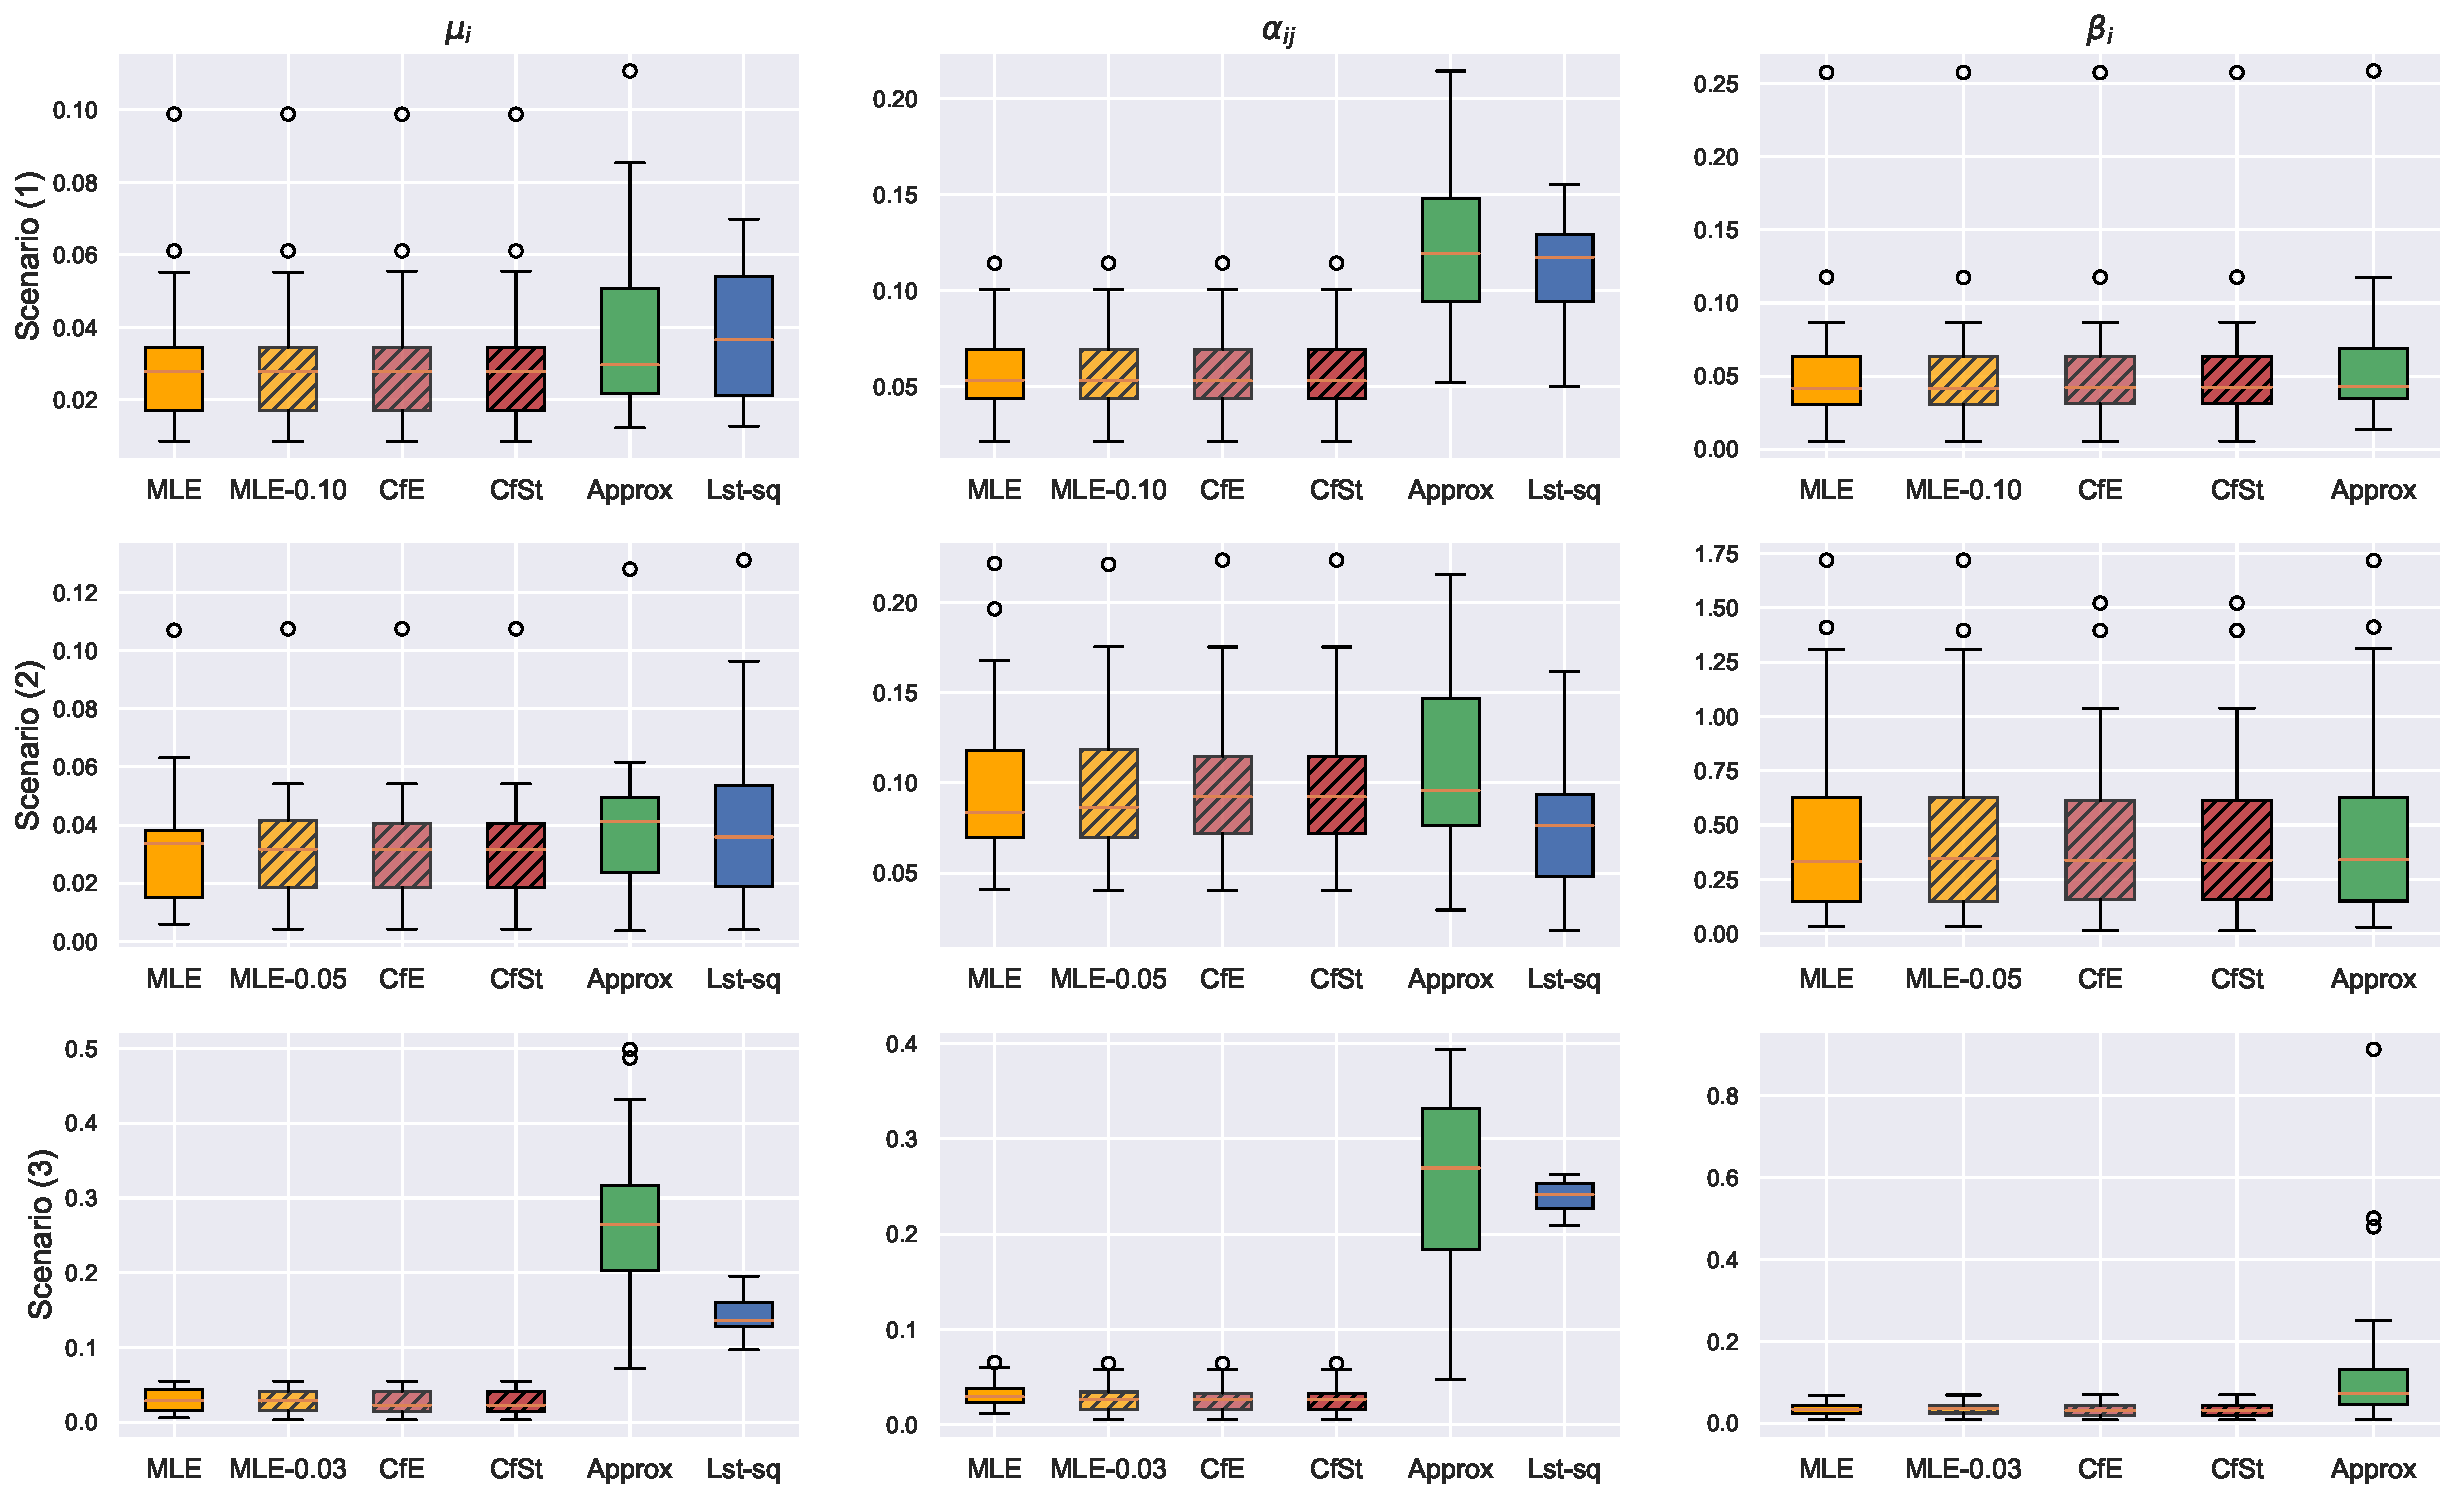
\includegraphics[width=0.9\linewidth]{images/chapter3/boxplots2O.pdf}
    \caption{Boxplots of the relative squared error for each group of parameters ($(\mu_i)_i$, $(\alpha_{i,j})_{i,j}$ and $(\beta_i)_i$) for 25 realisations of a two-dimensional Hawkes processes.
    (Lst-sq) does not appear in the last column because it is provided with the true values of \((\beta_i)_i\).
    The proposed methods are (MLE), (MLE-$\varepsilon$), (CfE) and (CfSt).}
    \label{fig:chap3_boxplots}
    \end{figure*}}
    
    First, we observe that delay factors \((\beta_i)_i\)
    (last column of Figure~\ref{fig:chap3_boxplots})
    are similarly estimated by all approaches.
    Let us recall that (Lst-sq) is not included in the comparison of delay factors:
    since it requires to provide a value for these parameters (they are not estimated),
    it was given the true values of \((\beta_i)_i\) as input.
    An alternative offered by \texttt{tick} is to provide a grid
    of values, but this approach, denoted (Grid-lst-sq), is included in the comparison at the end of the section because of its difference with the exponential model considered here.
    
    Then, regarding the baseline intensities \((\mu_i)_i\) and the interaction factors \((\alpha_{ij})_{ij}\),
    the proposed methods outperform the two other approaches.
    In all Scenarios, (MLE-$\varepsilon$), (CfE) and (CfSt) appear to perform almost identically as they retrieve the same supports and from then, the re-estimations are the same.
    In Scenario~(2), all estimation methods perform reasonably well. 
    This can be explained by the weak inhibiting effect of the interaction $1\to2$, leaving the intensity almost always positive.
    The slight difference between (MLE-$\varepsilon$) and the confidence intervals comes from the fact that (MLE-$\varepsilon$) is applied individually to each estimation so for some estimations it does not set any values to zero.
    
    
    In Scenario~(1), the performance of (Approx) and (Lst-sq) is altered, in particular for the \((\tilde \alpha_{ij})_{ij}\) estimations, because the inhibiting effect is stronger than in Scenario~(2).
    The major changes appear in Scenario~(3), where both (Approx) and (Lst-sq) obtain very high relative errors.
    More precisely, they fail to explain the interactions between the two processes (see the estimations \((\tilde \alpha_{ij})_{ij}\) in the middle column of Figure~\ref{fig:chap3_boxplots}), which is compensated by a wrong estimation \((\tilde \mu_i)_i\) of baseline intensities.
    This is not surprising since Scenario~(1), and even more Scenario~(3), were designed so that the intensity functions are frequently equal to zero, which induces major differences between true and underlying intensities.
    Since (Approx) and (Lst-sq) are both based on assuming that these two functions are almost equal, the violation of this assumption causes large estimation errors.
    As expected, the proposed methods, which are developed to handle such inhibiting scenarios, provide accurate estimations.
    
    These results are confirmed by the outcomes of the goodness-of-fit test displayed in Table~\ref{tab:chap3_p_values_2}.
    It shows indeed the averaged $p$-values for each scenario using both the true parameters and all four estimations from Figure~\ref{fig:chap3_boxplots} with 25 simulations different from the ones used for estimation. In particular, we can see that our methods obtain high $p$-values, being very close to those obtained using the true parameters.
    Table~\ref{tab:chap3_p_values_2} also highlights when parameters are incorrectly estimated.
    For instance, in Scenario (1), (Approx) correctly estimate Process~2 but provides less accurate estimations for Process~1 (the \(p\)-value is almost half the one obtained with the true parameters), which is the one characterised by a self-inhibiting behaviour.
    In addition, at least one of the proposed methods obtains the highest value for $p_{tot}$ in each scenario, which illustrates the ability of these procedures to reconstruct the complete process $N$.
    Let us note that the very low \(p\)-values obtained by (Approx) and (Lst-sq) for Scenario (3) confirm the ability of the goodness-of-fit procedure to detect when the parameter estimations strongly differ from the true parameters.
    
    \begin{table*}[!ht]
    \begin{center}
    \centering
    \begin{tabular}{c|ccc|ccc|ccc}
          & \multicolumn{3}{c|}{Scenario (1)}& \multicolumn{3}{c|}{Scenario (2)}& \multicolumn{3}{c}{Scenario (3)} \\
         $p$-value & $p_1$ & $p_2$ & $p_{tot}$ & $p_1$ & $p_2$ & $p_{tot}$ & $p_1$ & $p_2$ & $p_{tot}$\\
         \toprule
         True & 0.492 & 0.438 & 0.430 & 0.535 & 0.468 & 0.479 & 0.510 & 0.623 & 0.338\\
         \midrule
         MLE &  0.440 & 0.442  & 0.398  & 0.483  & 0.461  & 0.485 & 0.549  & 0.638 & $0.357$\\
         \midrule
         MLE-$\varepsilon$ & \multirow{3}{*}{0.440} & \multirow{3}{*}{0.442} &  \multirow{3}{*}{0.398} & \multirow{3}{*}{0.488}  & \multirow{3}{*}{0.461} & \multirow{3}{*}{0.491} & \multirow{3}{*}{0.549} & \multirow{3}{*}{0.574}  & \multirow{3}{*}{0.327}  \\
         CfE &  &  &  &  &  &  &  &  &  \\
         CfSt &  &  &  &  &  &  &  &  &  \\
         \midrule
         Approx & 0.257 & 0.442 & 0.358 & 0.483 & 0.452 & 0.459 & $\mathbf{0.0}$ & $\mathbf{0.007}$ & $\mathbf{0.0}$ \\
         Lst-sq & 0.154 & 0.438 & 0.392 & 0.534 & 0.463 & 0.478 & $\mathbf{0.0}$ & $\mathbf{0.0}$ & $\mathbf{0.0}$
    \end{tabular}
    \caption{Average $p$-values for estimations of two-dimensional Hawkes processes for all scenarios. The values are averaged over 25 simulations. In bold the $p$-values correspond to a rejected hypothesis at a confidence level of $0.95$.}
    \label{tab:chap3_p_values_2}
    \end{center}
    \end{table*}

     Lastly, let us investigate the estimations obtained via (Grid-lst-sq), which can be used in practice as a way to estimate the parameters $\beta_i$ by providing a grid of possible parameters.
     Let us mention that both of the previous comparisons (boxplots and \(p\)-values) cannot be done here due to the difference in the number of parameters, but we can compare the methods in terms of
     reconstructions $\tilde h_{ij}$ of the interaction functions $h_{ij}$.
     For this purpose, we analyse Figure~\ref{fig:chap3_reconstruction_param_1}, which represents the estimated interaction functions \(\tilde h_{ij}\) for all methods in Scenario (3).
     Interestingly, we see that (Grid-lst-sq) performs similarly to (Lst-sq),
     while the latter is fed with all true values \((\beta_i)_i\) for each interaction.
     However, we see that (Grid-lst-sq)  suffers from the same difficulties than (Approx) and (Lst-sq), which was expected since it relies on the same unvalid assumption.
     Let us note that we chose to display the results for Scenario (3) since it highlights the main differences between the compared approaches but the reconstructions for Scenarios (1) and (2)
     can be found in Appendix~\ref{app:chap3_numerical}
     (Figures \ref{fig_supp:scenario_1} and \ref{fig_supp:scenario_2}).
     
     {\begin{figure*}[!ht]
     \centering
     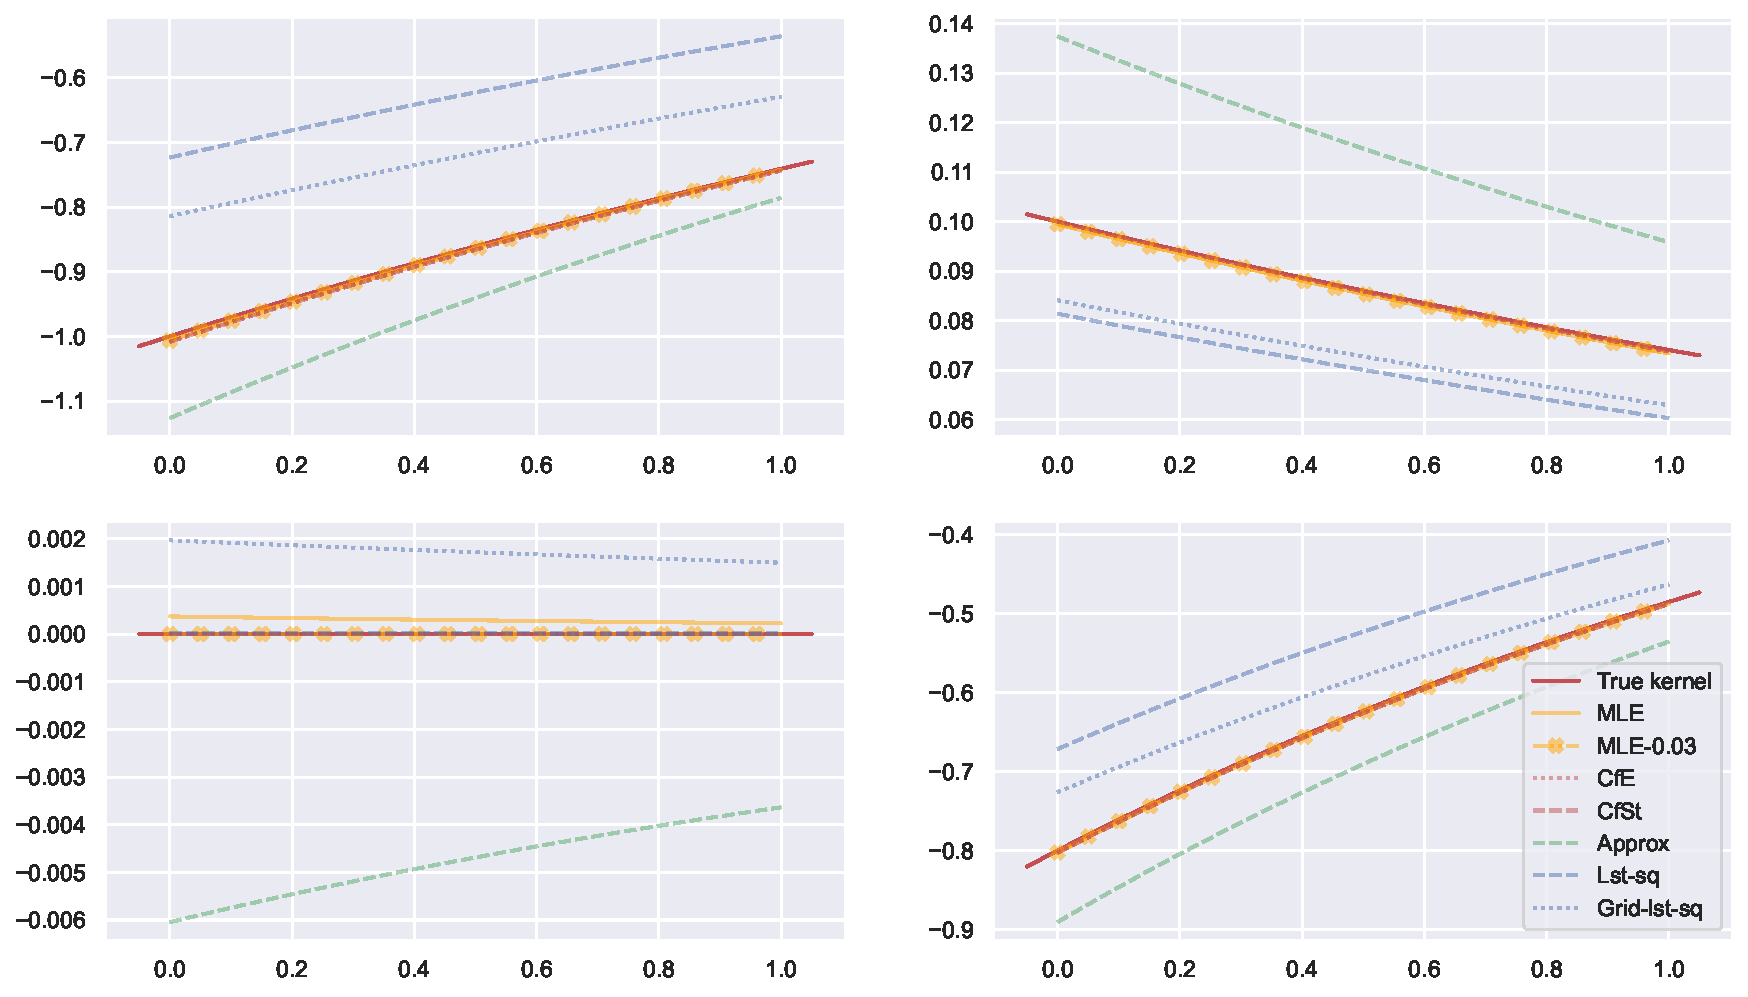
\includegraphics[width=0.9\linewidth]{images/chapter3/reconstruction_param_3.pdf}
     \caption{Reconstruction of interaction functions $h_{ij}$ for Scenario (3) of two-dimensional Hawkes processes along with all estimated functions $\tilde h_{ij}$. The real function is plotted in red and 25 estimations are averaged for each method.}
     \label{fig:chap3_reconstruction_param_1}
     \end{figure*}}


  \subsubsection{A $10$-dimensional Hawkes process}
    A \(10\)-dimensional Hawkes process is simulated based on a set of parameters corresponding to the quantities $(\sign(\alpha_{ij})\|h_{ij}\|_1)_{ij} = (\alpha_{ij}/\beta_i)_{ij}$ displayed in Figure~\ref{fig:chap3_heatmap_10}.
    The chosen parameters fulfil the existence condition $\|\rho(S^+)\| < 1$.

    {\begin{figure*}
    \centering
    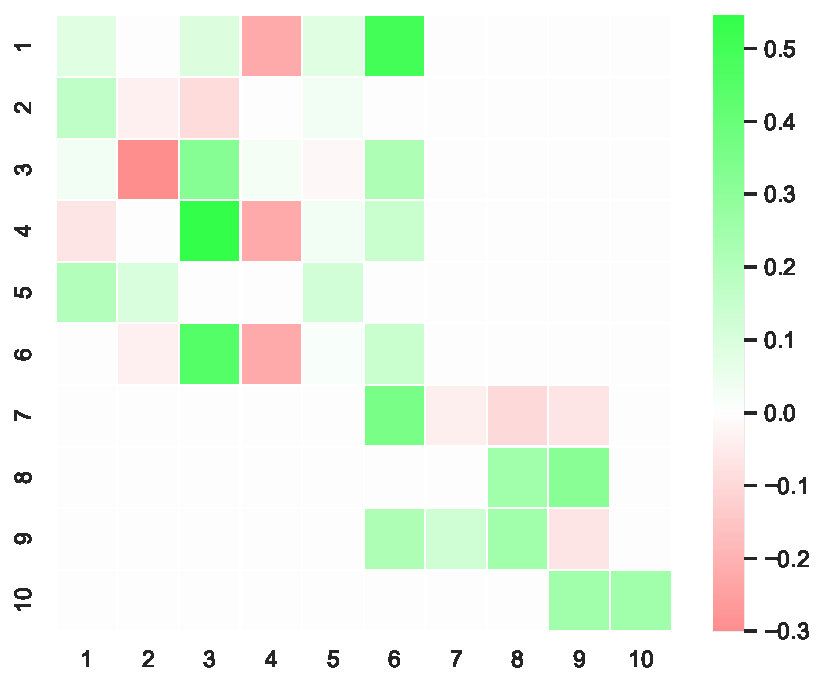
\includegraphics[clip,width=0.75\linewidth]{images/chapter3/Realheat.pdf}
    \caption{Heatmap of real parameters $(\sign(\alpha_{ij})\|h_{ij}\|_1)_{ij} = (\alpha_{ij}/\beta_i)_{ij}$ for the $10$-dimensional simulation.}
    \label{fig:chap3_heatmap_10}
    \end{figure*}}
    {\begin{figure*}
    \centering
    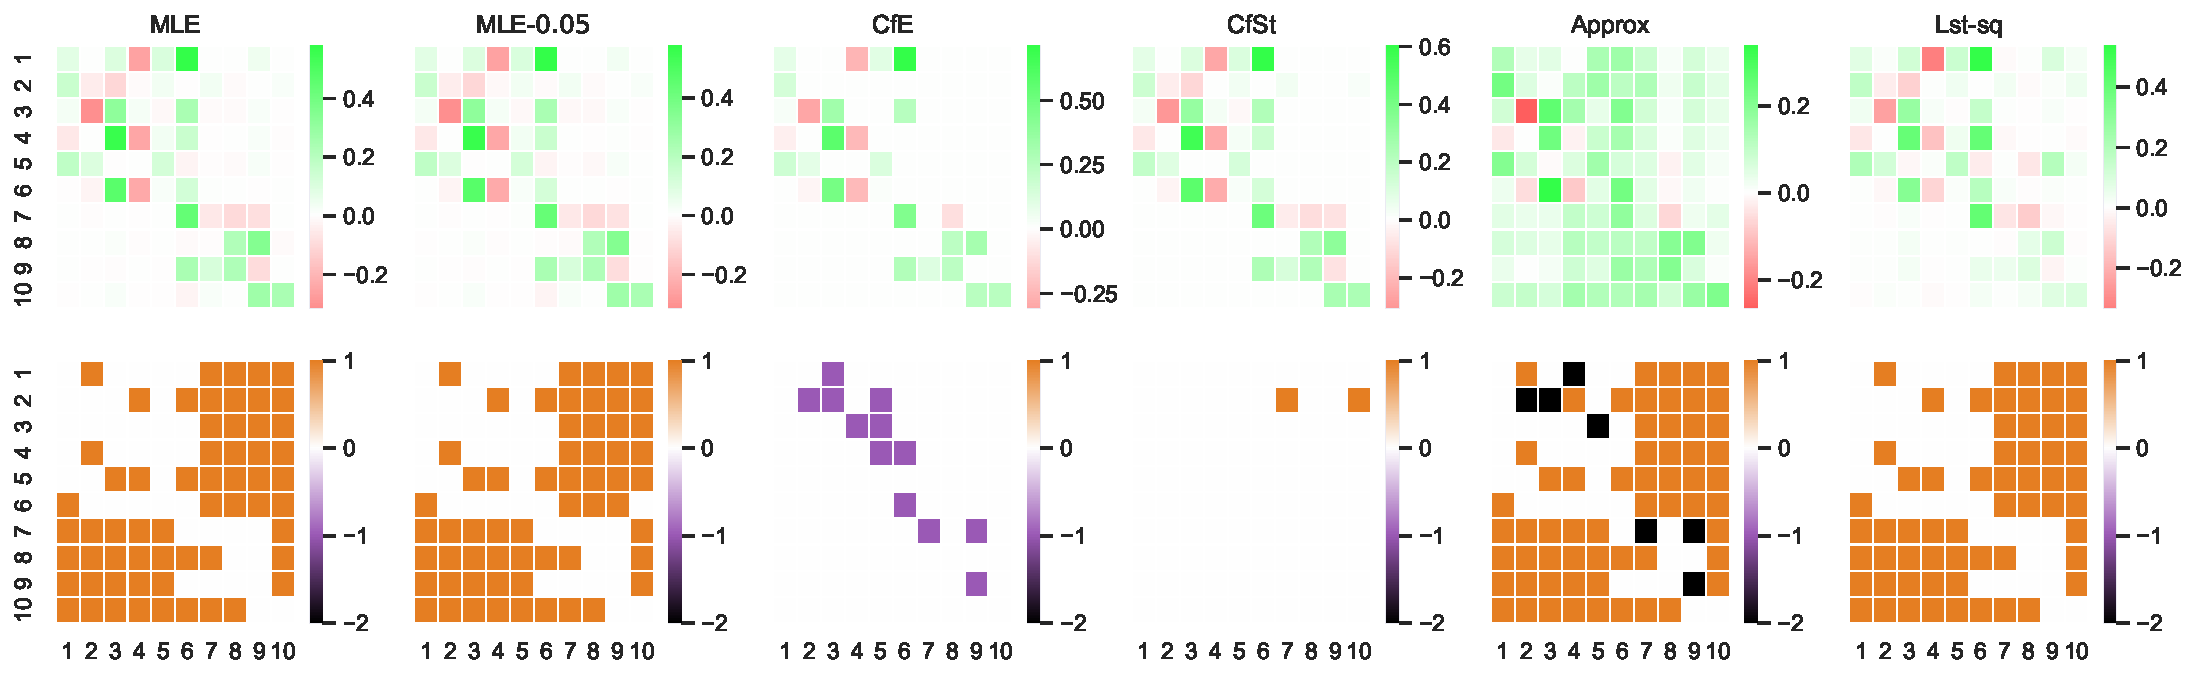
\includegraphics[clip, width=\linewidth]{images/chapter3/heatmap_hori.pdf}
    \caption{Top row corresponds to the heatmap for each estimation method. Bottom row corresponds to errors made with respect to real parameters from Figure \ref{fig:chap3_heatmap_10}. A value of 1 (orange) shows an undetected 0 (non-null estimation for $\alpha_{ij} = 0$), a value of -1 (purple) shows a non-null value set to 0 and a value of -2 (black) shows a non-null value whose sign is wrongly estimated. Each of the compared approaches is described in Section \ref{sec:chap3_description_methods}.}
    \label{fig:chap3_heatmap_estimated}
    \end{figure*}}

    The corresponding estimations \(\tilde \alpha_{ij}\) and \(\tilde \beta_{i}\) are averaged over 25 realisations and displayed in Figure~\ref{fig:chap3_heatmap_estimated}.
    The heatmap representation is convenient for high-dimensional processes as it allows us to see whether the signs of each interaction are well-estimated and whether the null-interactions are correctly detected.


    In this example we decided to keep only (Approx) and (Lst-sq) as comparison methods as these are the ones with the same parameterisation for the kernel functions.
    Among the four methods considered, (Approx) is the only one that wrongly estimates the sign of some interactions, represented by the black boxes in the second row matrix. (MLE) and (Lst-sq) correctly retrieve the sign of each interactions but are unable to detect the null interactions: this is not surprising since (MLE) does not contain a regularisation step and the (Lst-sq) estimator is implemented with a $\ell_2$-penalty which does not provide a sparse solution.
    On the one hand, (MLE-$\varepsilon$) is in this case quite conservative by setting a single value equal to 0 compared to (MLE).
    On the other hand, both confidence intervals methods improve the number of interactions whose sign is correctly estimated. Interestingly, we see that (CfE) sets more values equal to zero than it should (purple boxes) whereas (CfSt) denotes the opposite effect by not detecting null interactions (orange boxes). Overall, (CfSt) obtains the best results in terms of support recovery and sign estimations by committing only two errors. Table~\ref{tab:chap3_p_values_10} summarises the $p$-values for each hypothesis as described in Section~\ref{sec:chap3_goodness}. 
    All of the proposed methods obtain overall better $p$-values with no particularly low values, which is not the case for (Approx) (see $p_4$ and $p_{tot}$) and for (Lst-sq) (see $p_8$ and $p_{10}$). Although the $p$-values all exceed $5\%$, they remain substantially smaller than those obtained with the alternative methods.  
    
    \begin{table*}[!ht]
    \begin{center}
    \setlength{\tabcolsep}{5pt}
    \centering
    \begin{tabular}{c|cccccccccc|c}
         $p$-value & $p_1$ & $p_2$ & $p_3$ & $p_4$ & $p_5$ & $p_6$ & $p_7$ & $p_8$& $p_9$ & $p_{10}$ & $p_{tot}$\\
         \toprule
         True & 0.437 & 0.608 & 0.435 & 0.517 & 0.534 & 0.45 & 0.43 & 0.47 & 0.533 & 0.509 & 0.464\\
         \midrule
         MLE & 0.451 & 0.619 & 0.399 & 0.466 & 0.506 & 0.464 & 0.424 & 0.386 & 0.45 & 0.483 & 0.434\\
         \midrule
         MLE-0.05 & 0.454 & 0.622 & 0.392 & 0.466 & 0.505 & 0.427 & 0.418 & 0.392 & 0.495 & 0.482 & 0.432 \\
         CfE & 0.424 & 0.532 & 0.393 & 0.528 & 0.532 & 0.301 & 0.444 & 0.427 & 0.516 & 0.505 & 0.439\\
         CfSt & 0.452 & 0.633 & 0.375 & 0.474 & 0.527 & 0.462 & 0.431 & 0.422 & 0.488 & 0.493 & 0.465\\
         \midrule
         Approx & 0.411 & 0.376 & 0.475 & 0.077 & 0.485 & 0.411 & 0.3 & 0.384 & 0.285 & 0.436 & 0.085\\
         Lst-sq & 0.422 & 0.63 & 0.344 & 0.456 & 0.416 & 0.439 & 0.411 & 0.096 & 0.579 & 0.157 & 0.423\
    \end{tabular}    
    \caption{$p$-values for estimations of a ten-dimensional Hawkes process. The values are averaged over 25 simulations. $p_{tot}$ corresponds to testing whether the estimated intensity function corresponds to a multivariate Hawkes process $N$ as defined in Section \ref{sec:chap3_goodness}.}
    \label{tab:chap3_p_values_10}
    \end{center}
    \end{table*}

Finally, we compare the relative squared errors for each group of parameters (see Figure \ref{fig:chap3_errors_10_dim}). Similarly to the two-dimensional case, all proposed methods perform significantly better than alternative approaches regarding the estimation of all parameters.
In addition, it can be noticed that inaccurate estimations of the parameters $\alpha_{ij}$ tend to deteriorate the estimations of $\mu_i$, which suggests an effect of compensation between these parameters.
Regarding the estimator (CfSt), which shows the best averaged performance, it can be remarked that it also exhibits a large variance, in particular when estimating $\beta_i$. 

Figure~\ref{fig:chap3_p_values_support} illustrates for (CfST) the ordered $p$-values for hypothesis $\mathcal{H}_0 : \alpha_{ij} = 0$.

{\begin{figure}[!ht]
     \centering
     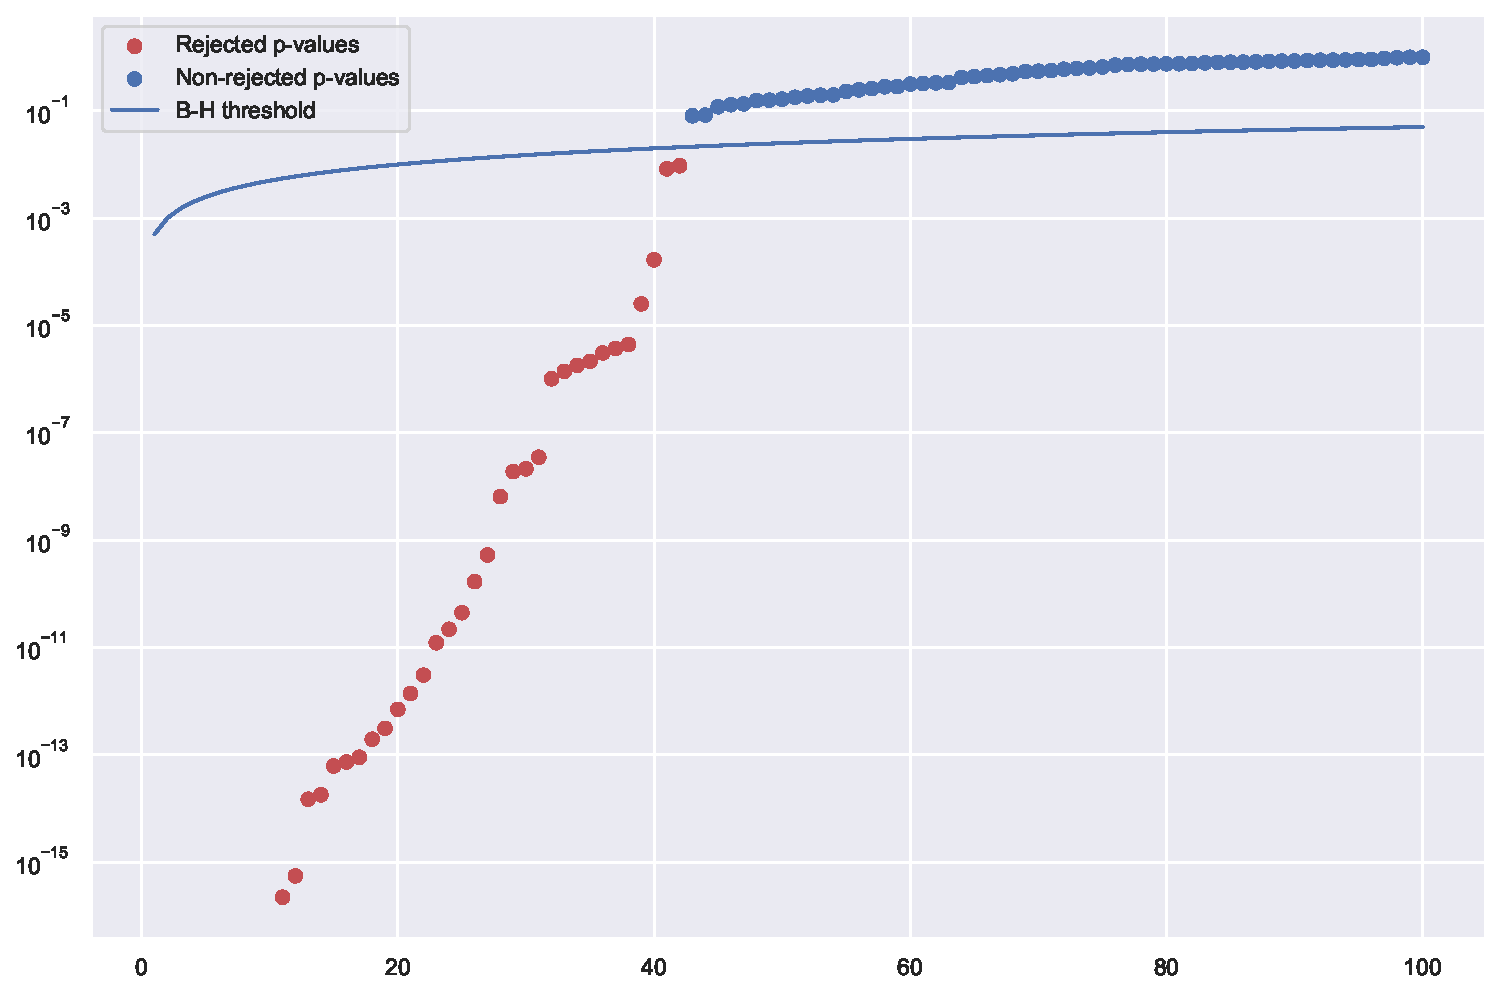
\includegraphics[width=0.75\linewidth]{images/chapter3/p_values_10.pdf}
     \caption{Ordered $p$-values corresponding to support estimation of method (CfSt). Red points correspond to rejected null hypothesis $\mathcal{H}_0 : \alpha_{ij} = 0$ and blue points to non-rejected ones.}
     \label{fig:chap3_p_values_support}
     \end{figure}}

This can be explained by this estimator providing a very sparse solution (as seen in Figure \ref{fig:chap3_heatmap_estimated}) and therefore taking into account less observations for estimating the coefficients $\beta_i$.

{\begin{figure*}[!ht]
     \centering
     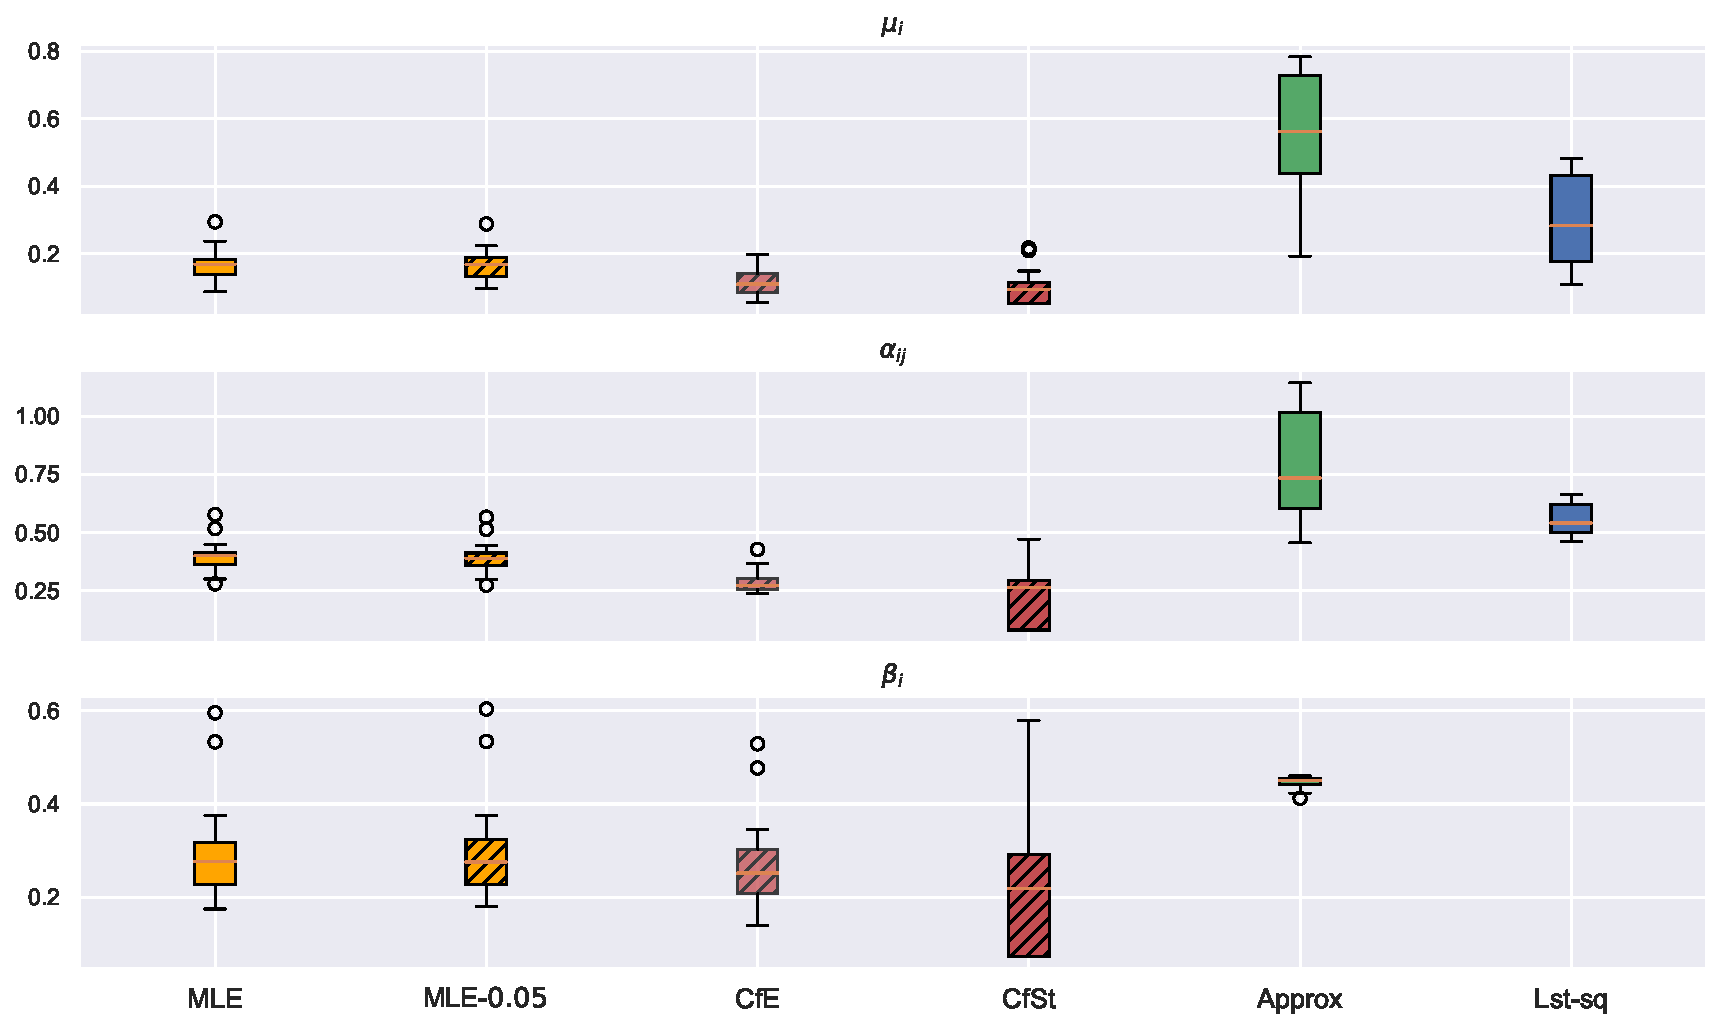
\includegraphics[width=0.9\linewidth]{images/chapter3/boxplots_10_dim.pdf}
     \caption{Boxplots of the relative squared error for each group of parameters ($(\mu_i)_i$, $(\alpha_{ij})_{i,j}$ and $(\beta_i)_i$) for 25 realisations of a ten-dimensional Hawkes processes.
    (Lst-sq) does not appear in the last row because it is provided with the true values of \((\beta_i)_i\).
    The proposed methods are (MLE), (MLE-$\varepsilon$), (CfE) and (CfSt).}
     \label{fig:chap3_errors_10_dim}
     \end{figure*}}

An important question for any inference method, especially in a high-dimensional setting, is its computational cost. Table~\ref{tab:chap3_times_10} shows the average estimation time (over 25 realisations), all times being total estimation time. More precisely, for our 3 model selection methods (MLE-$\varepsilon$), (CfE) and (CfSt), it takes into account the total times, including the first (MLE) estimation in addition to the re-estimation over the support. 

\begin{table*}[!ht] 
    \begin{center}
    \setlength{\tabcolsep}{2pt}
    \centering
    \begin{tabular}{c|c|ccc|c|cc}
          & MLE & MLE-$\varepsilon$ & CfE & CfSt & Approx & Lst-sq & Grid-lst-sq\\
         \toprule
         Computing time & 87.6 & 178.2 & 147.2 & 152.2 & 51.4 & 1.32 & 47.7
    \end{tabular}
    \caption{Average computing time in seconds for all estimation methods, averaged over 25 realisations of a ten-dimensional Hawkes process.  The time shown for (MLE-$\varepsilon$) is the total time of estimation for 7 different values of $\varepsilon$. Similarly for \texttt{tick} methods, the time is for 7 different levels of penalisation (as done in the estimations of Section~\ref{sec:chap3_dim2}). For the (Grid-lst-sq), we provided a search grid for $\beta_i$ that contains 12 values, including the true one.}
    \label{tab:chap3_times_10}
    \end{center}
    \end{table*}

Although the difference between (Lst-sq) and all other methods is substantial, let us recall that (Lst-sq) requires to be provided with parameters $\beta_i$, which offers two numerical advantages: it does not need to optimise for parameters $\beta_i$ which are the more difficult parameters to estimate and it includes a pre-computation step (of exponential terms) that accelerates all internal computations. In order to provide a fairer comparison, we include the computing time of the (Grid-lst-sq) method which can be considered as an alternative for estimating these parameters when given a search grid for $\beta_i$ (here with 12 values, including the true parameters).
As expected, the computational cost of the MLE method is higher than the alternative approaches (Approx) and (Grid-lst-sq), designed for the linear model.
It remains nevertheless that (Lst-sq) and (Grid-lst-sq) are both implemented in a compiled language (C++), which is always faster than an interpreted language such as that used in the proposed package (Python).
However, all computation times remain quite reasonable, even for the methods that include a selection model step. 

\subsection{Robustness on misspecified models}
In this section, we address the question of the robustness of our estimator regarding the misspecification of the kernel function. More precisely, we generate a two-dimensional Hawkes process with power-law kernels, which are commonly used in the literature \parencite{Mishra2016, Ogata1988} as an alternative to the exponential kernel for modelling a slower convergence to zero. For all $i, j$ we define the power-law kernel as: \[h_{ij}(t) = \frac{\alpha_{ij}\beta_{ij}}{(1 + \beta_{ij}t)^{1 + \gamma}}\,,\] with $\beta_{ij} > 0$, $\gamma > 0$ and $\alpha_{ij}\in\RR$ in order to allow inhibition effects. Let us remark that in the general case each kernel function could be given a different parameter $\gamma_{ij}$ but here we fix the same parameter for all interactions, which is a similar condition as Assumption~\ref{assu:chap3_beta}.

We propose to investigate different scenarios in order to model different behaviours. In all cases, we set the values of $\alpha_{ij}$ in order to have both excitation and inhibition effects and the values of $\mu_i$ as follows:
\[
 \begin{pmatrix}
  \mu_{1} \\
  \mu_{2} 
  \end{pmatrix} =
  \begin{pmatrix}
  1.0 \\ 
  1.0
  \end{pmatrix}\,,
  \quad
  \begin{pmatrix}
  \alpha_{11} & \alpha_{12}\\
  \alpha_{21} & \alpha_{22}
  \end{pmatrix}=
  \begin{pmatrix}
  0.1 & 1.5\\
  1.0 & -0.5
  \end{pmatrix}\,.
\]

\begin{itemize}
    \item  Scenarios $\gamma$ : we set
    
    \[\begin{pmatrix}
  \beta_{11} & \beta_{12}\\
  \beta_{21} & \beta_{22}
  \end{pmatrix}=
  \begin{pmatrix}
  1.0 & 1.1\\
  1.2 & 1.0
  \end{pmatrix}\ ,
\]
    
all values being similar in order to be close to Assumption~\ref{assu:chap3_beta}. Then we study the effect of parameter $\gamma$ which controls how the kernel functions decrease to zero. We set \[\gamma\in\{2.0, 4.0, 6.0, 8.0\}\,.\]


    \item Scenario $\beta$ : we keep the same values of $\mu_i$, $\alpha_{ij}$ as in Scenarios $\gamma$, we fix $\gamma=4.0$ and we choose very different values of $\beta_{i,j}$:
    
    
 \[\begin{pmatrix}
  \beta_{11} & \beta_{12}\\
  \beta_{21} & \beta_{22}
  \end{pmatrix}=
  \begin{pmatrix}
  1.0 & 2.0\\
  0.1 & 1.0
  \end{pmatrix}\,,
\]
    
    
    
    so that Assumption~\ref{assu:chap3_beta} is violated and therefore the intensity function of process $N^2$ is frequently non-monotonous between two event times.

\end{itemize}

We expect that our estimator should adapt better to Scenarios $\gamma$ (in particular large values of $\gamma$ would correspond to a fast convergence to zero) than to Scenario $\beta$.

Figure~\ref{fig:chap3_heatmap_powerlaw} represents the heatmap for $\sign(\alpha_{ij})\| h_{ij} \|_1 = \alpha_{ij}/\gamma$ and $\sign(\tilde \alpha_{ij})\| \tilde h_{ij}\|_1 = \tilde \alpha_{ij}/ \tilde\beta_{i}$ as well as whether the type of each interaction is correctly estimated (excitation or inhibition). We first notice that in most cases, our method is robust enough to differentiate between exciting and inhibiting interactions, the only errors concerning parameter $\alpha_{11}$ that is close to zero. For Scenarios $\gamma$, we can observe as expected that the bigger differences are obtained for smaller values of $\gamma$. Although the signs of the interactions are correctly estimated in Scenario $\beta$, we can observe substantial errors regarding the estimations of both $\alpha_{21}$ and $\alpha_{22}$. 

{\begin{figure*}[!ht]
     \centering
     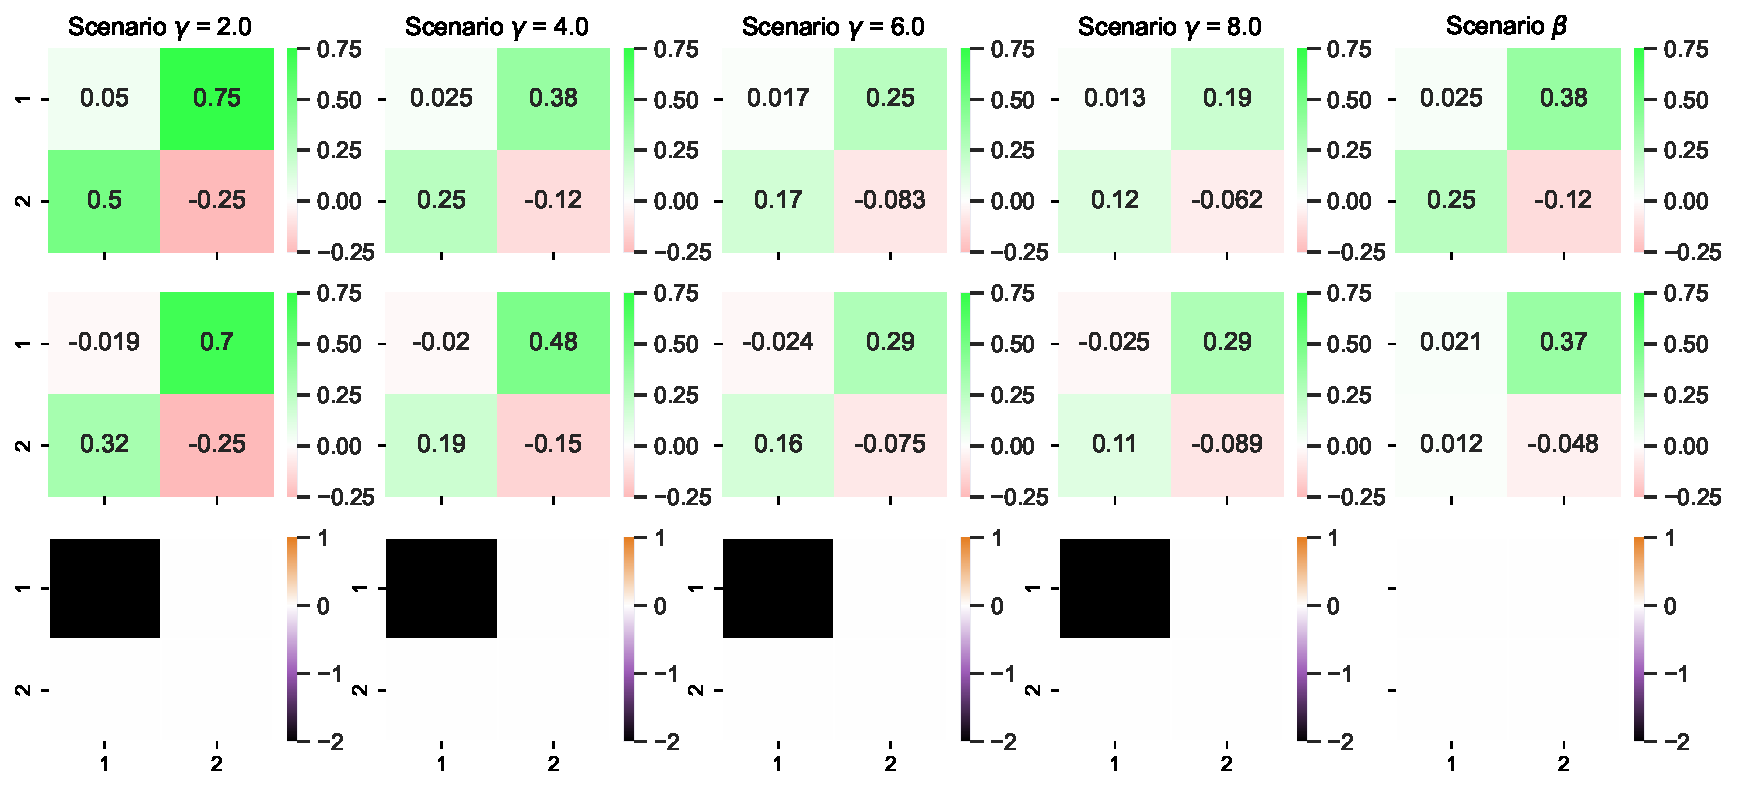
\includegraphics[width=0.9\linewidth]{images/chapter3/heatmap_powerlaw_both.pdf}
     \caption{Top row corresponds to the heatmap $\sign(\alpha_{ij})\| h_{ij} \|_1 = \alpha_{ij}/\gamma$. Middle row corresponds to the estimated heatmap $\sign(\tilde \alpha_{ij})\| \tilde h_{ij}\|_1 = \tilde \alpha_{ij}/ \tilde\beta_{i}$. Bottom row corresponds to errors when estimating the nature of the interaction. A black box represents a value $\alpha_{ij}$ whose sign is wrongly estimated.}
     \label{fig:chap3_heatmap_powerlaw}
     \end{figure*}}

Table~\ref{tab:chap3_p_values_powerlaw} shows the average $p$-values associated with the goodness-of-fit measure presented in Section~\ref{sec:chap3_goodness}. It confirms that for all Scenarios $\gamma$, the $p$-values are smaller for smaller values of $\gamma$, all $p$-values remaining greater than 5\%. However, the $p$-values associated with Scenario $\beta$ are always equal to zero, which means that the goodness-of-fit is able to detect that the interactions are not correctly estimated. 

\begin{table}[!ht]
    \begin{center}
    \centering
    \begin{tabular}{c|c|ccc}
         \multicolumn{2}{c}{} & $p_1$ & $p_2$ & $p_{tot}$\\
         \toprule
         \multirow{5}{*}{Scenario $\gamma$} & $\gamma = 2.0$ & 0.140 & 0.275 & 0.068\\
         & $\gamma = 4.0$ & 0.484 & 0.536 & 0.482\\
         & $\gamma = 6.0$ & 0.381 & 0.503 & 0.408\\
         & $\gamma = 8.0$ & 0.408 & 0.506 & 0.330\\
         \midrule
         \multicolumn{2}{c|}{Scenario $\beta$} & \textbf{0.0} & \textbf{0.0} & \textbf{0.0}
    \end{tabular}
    \caption{Average $p$-values for estimations of two-dimensional Hawkes processes for all scenarios in the misspecified power-law model. The values are averaged over 25 simulations. In bold the $p$-values correspond to a rejected hypothesis at a confidence level of $0.95$.}
    \label{tab:chap3_p_values_powerlaw}
    \end{center}
    \end{table}


To conclude, if the true model is not too far from an exponential model and Assumption~\ref{assu:chap3_beta} holds, our procedure can adapt and provide reasonable estimations. If not, our estimator cannot adjust but we are able to detect incorrect estimations thanks to the goodness-of-fit procedure.


\section{Application on neuronal data}\label{sec:chap3_neuron}

\subsection{Preprocessing and data description}

In this section we present the results obtained by our estimation method applied to a collection of 10 trials consisting in the measurement of spike trains of 223 neurons from the lumbar spinal of a red-eared turtle. This data are first presented in  \textcite{Petersen2016} and then also analysed in \textcite{Bonnet2022bis} to study how the activity of a group of neurons impacts the membrane potential's dynamic of another neuron. In particular, recovering the connectivity graph allows to isolate a subnetwork which activity impacts the dynamics of one given neuron.  Events were registered for 40 seconds and in order to take into account eventual stationarity we only consider the events that took place on the interval $[11, 24]$ (see \textcite{Bonnet2022bis} for further details).  Among all trials, each neuron recording contains between 54 and 4621 event times. Furthermore, we divide our samples in a training set consisting on all events in half the interval $[11, 17.5]$ and a test set consisting on the remaining window $[17.5, 24]$, in particular each neuron has at least 15 event times in each set. The training sets are used for obtaining the estimations and the test sets for performing the goodness-of-fit tests. 

\subsection{Resampling}

As only ten realisations are available, this can obviously limit the performance of both confidence intervals methods. In order to counter this problem, we perform a resampling method obtained as follows:
\begin{enumerate}
	\item We sample 3 realisations at random $(N_1, N_2, N_3)$, without replacement and by taking the order into account. From now on, we consider that each realisation takes place in the time interval $[0,6.5]$ (instead of $[11, 17.5]$).
	\item We cumulate all 3 realisations by considering that process $N_1$ takes place in $[0, 6.5]$ then process $N_2$ in $[6.5, 13]$ and finally $N_3$ in $[13, 19.5]$. This creates a single realisation $N$ in the interval $[0, 19.5]$. 
\end{enumerate}

This approach is proposed in \textcite[Section 3.4]{Reynaud2014}. In our case, we repeat this process 20 times to obtain another sample of realisations. These new sample will be used for both the (MLE) method (presented as (resampled-MLE)) and for both (CfE) and (CfSt).


\subsection{Goodness-of-fit and multiple testing procedure}

Since we are dealing with a high-dimensional setting, it is crucial to account for a multiple testing correction which is performed through the Benjamini-Hochberg procedure as described in Section \ref{sec:chap3_support}. In this case, the adapted rejection threshold corresponds to $\frac{0.05 k}{d+1}$ and represented in Figure \ref{fig:chap3_p_values_neurons} by a blue line.
This is particularly useful in order to determine the best value of $\varepsilon$ for (MLE-$\varepsilon$) as we do not have prior knowledge regarding the sparsity of the neuronal connections.

{\begin{figure*}[!ht]
\centering
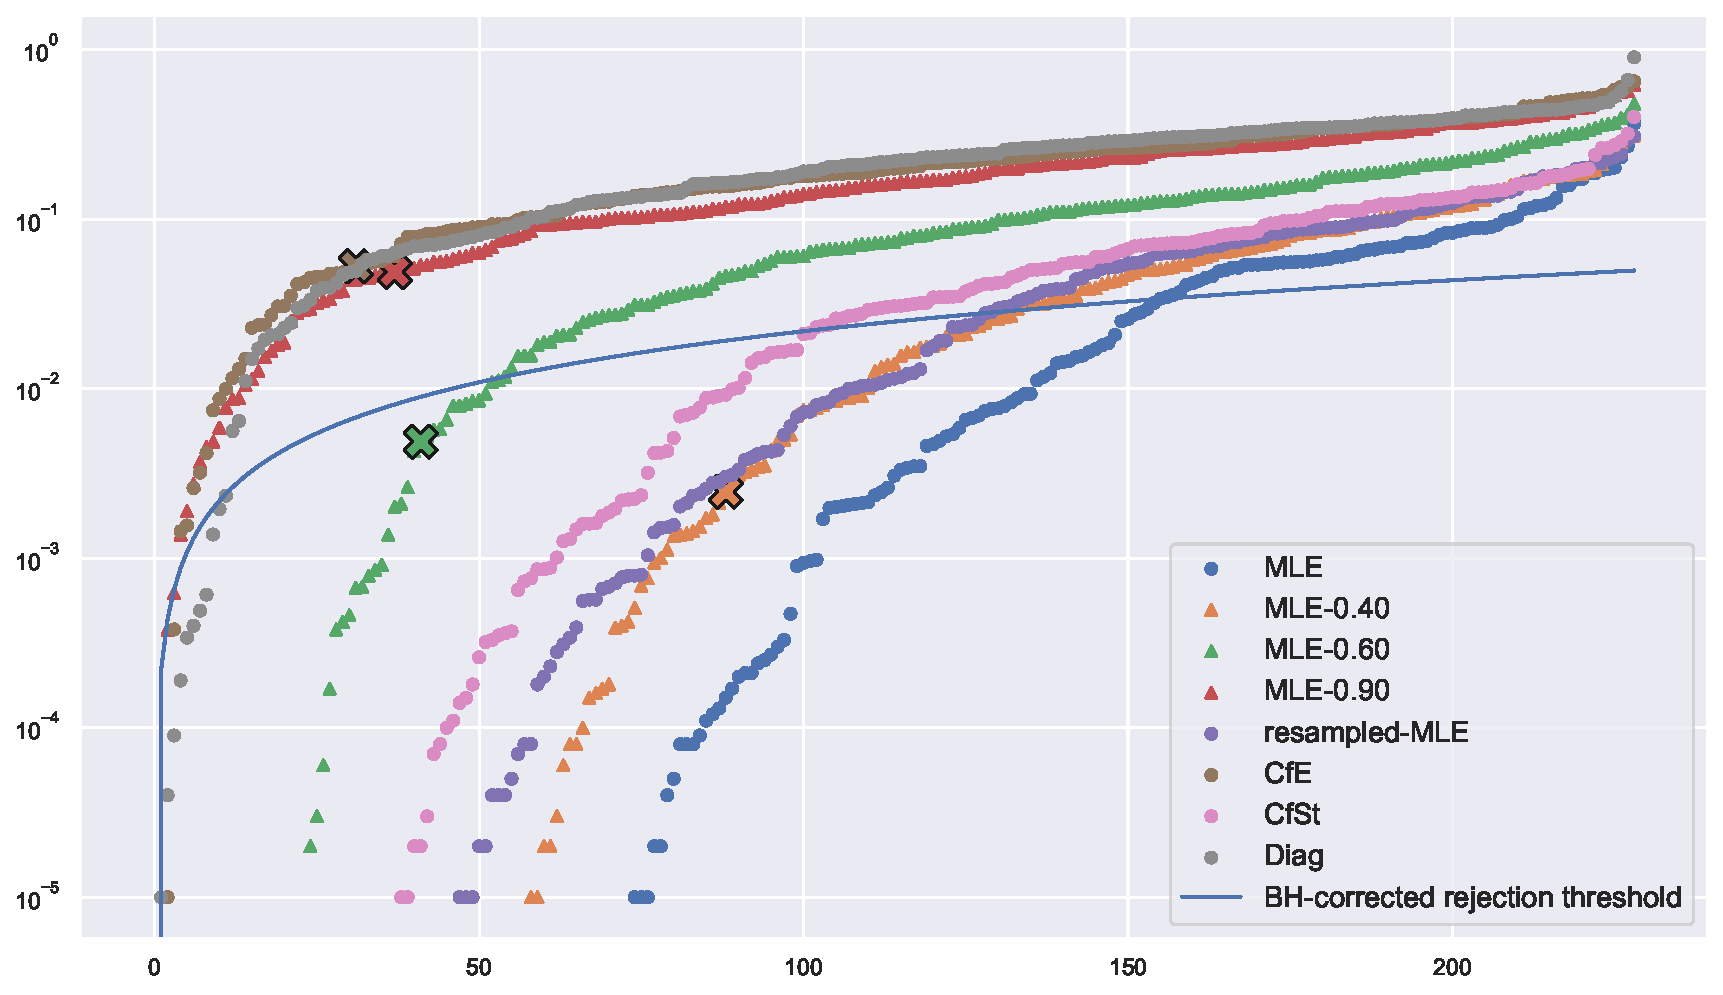
\includegraphics[width=0.9\linewidth]{images/chapter3/p_values_conf.pdf}
\caption{Ordered $p$-values for all hypothesis tests $\mathcal{H}_i$ and $\mathcal{H}_{tot}$. $p_{tot}$ appears as a cross for each model (if there appears no cross for one given method, it means that the corresponding $p_{tot}$ is equal to zero). The blue curve corresponds to the adapted rejection threshold from the B-H procedure, so all tests whose $p$-value are under the line are rejected.}
\label{fig:chap3_p_values_neurons}
\end{figure*}}

 Figure~\ref{fig:chap3_p_values_neurons} shows the ordered $p$-values for each hypothesis $\mathcal{H}_i$ along with hypothesis $\mathcal{H}_{tot}$ displayed with a bold cross, all total $p$-values also being summarised in Table~\ref{tab:chap3_p_tot_neurons}. 
    
    \begin{table*}[!ht] 
    \begin{center}
    \setlength{\tabcolsep}{2pt}
    \centering
    \begin{tabular}{c|c|ccc|ccc|c}
          & MLE & MLE-$0.40$ & MLE-$0.60$ & MLE-$0.90$ & resampled-MLE & CfE & CfSt & Diag\\
         \toprule
         $p_{tot}$ & 0.0 & 0.002 & 0.004 & \textbf{0.048} & 0.0 & \textbf{0.053} & 0.0 & 0.0
    \end{tabular}
    \caption{Values of $p_{tot}$ for each estimation method for the neuronal dataset. In bold appear the \(p\)-values above the rejection threshold after Benjamini-Hochberg procedure.}
    \label{tab:chap3_p_tot_neurons}
    \end{center}
    \end{table*}
    
 We first note that for most methods, the $p$-values $p_{tot}$ associated with the  $\mathcal{H}_{tot}$ hypothesis are either equal to 0 or under the rejection threshold. In particular, it is the case for the MLE-$\varepsilon$ approach for small values of $\varepsilon$ (i.e. weak sparsity scenarios) but as we increase the threshold $\varepsilon$, the $p$-values appear to increase, with the best estimation being achieved for $\varepsilon = 0.90$.
 
 This suggests that the simpler the model the better $p$-values we obtain so we decided to include another approach, named ``Diag'', consisting in setting all $\alpha_{ij} = 0$ for $i \neq j$. This corresponds to a model where there exists no interaction between neurons and we keep only self-interactions: in other words, each neuron is seen as a univariate Hawkes process with three parameters $(\mu_i,\alpha_{ii}, \beta_i)$. Although most hypotheses $\mathcal{H}_i$ are not rejected by the method, the total $p$-value $p_{tot}$ is zero which suggests that although such a model could explain each dimension individually, it is unable to explain the neurons' interactions as a whole interconnected process.
Although the total $p$-values are generally quite low, they remain above the rejection threshold for (MLE-$0.90$) and (CfE).
Let us notice that the high value of the best threshold (0.90) is consistent with the (CfE) estimator that provides an even sparser solution with $4.26\%$ non-null interactions. 

Let us also recall that the (CfSt) method relies on the assumption that the MLE estimator is asymptotically normal. Here we have a low number of repetitions ($10$ trials) in a high-dimensional setting where some neurons are rarely observed which could explain why this estimator does not perform well. Moreover, in this context, a Kolmogorov-Smirnov test of normality is likely to provide high $p$-values for such small-sized samples even for non-normal distributions.
 
 Finally, the model that best describes the complete process $N$ is (CfE) with the highest value for $p_{tot}$ and with almost all hypotheses, including $\mathcal{H}_{tot}$, not rejected. This suggests indeed that the estimations provided by (CfE) are the best fit for explaining the entire process as well as each individual subprocess.

\subsection{Estimation results} \label{sec:chap3_comment_neuron}
Figure~\ref{fig:chap3_heatmap_CfE} illustrates the obtained estimation for all parameters for the (CfE) method. 
Let us recall that the estimation for (CfE) is obtained by using the resampled trials: the support is determined by using the empirical quantiles confidence intervals after an estimation through (MLE) and then all parameters are re-estimated over each trial. A single estimation is obtained by averaging over all trials.

Although the heatmap matrix corresponding to $(\sign(\tilde\alpha_{ij}))_{ij}$ contains only $4.26\%$ of non-null entries, there remain many significant interactions. Interestingly, among them we detect all types of interactions: mutual excitation, mutual inhibition, self-excitation, self-inhibition. This supports the relevance of carefully accounting for inhibition when developing inference procedures.

We also notice that the diagonal contains mostly non-null entries (all but $6$), which highlights the major effect of self-interactions, among which some are negative and some are positive. Although it is possible that different neurons actually show different patterns, some being self-exciting and other self-inhibiting, there exists another hypothesis.  We might indeed observe a combination of effects from which we cannot distinguish: on the one hand, a self-exciting behaviour and on the other hand, a refractory period following a spike during which a neuron cannot spike again. This could also explain why the order of magnitude of the $\beta_i$ estimations, which describe the duration until an effect vanishes, is different from a neuron to another. It would be of great interest to propose another modelling that could account for both effects and thereby helping us to provide additional information to support or refute this hypothesis.

Another striking phenomenon is the behaviour of neuron $13$, which seems to interact with many other neurons: it contains indeed $69\%$ non-null receiving interactions (row) and $57\%$ non-null giving interactions (column). Further analysis shows that this neuron spikes only in one out of ten trials so that it could indicate an inaccurate estimation. However, the $p$-value associated with this neuron's subprocess is not rejected by our goodness-of-fit procedure, which suggests that the corresponding estimation is actually accurate. Therefore, this neuron could either play central role among the whole network or be connected to an unobserved neuron with a central role. On the opposite side, some neurons exhibit only a few connections, in particular there is one neuron that only receives interactions without giving, while another one gives without receiving.

{\begin{figure*}[!ht]
\centering
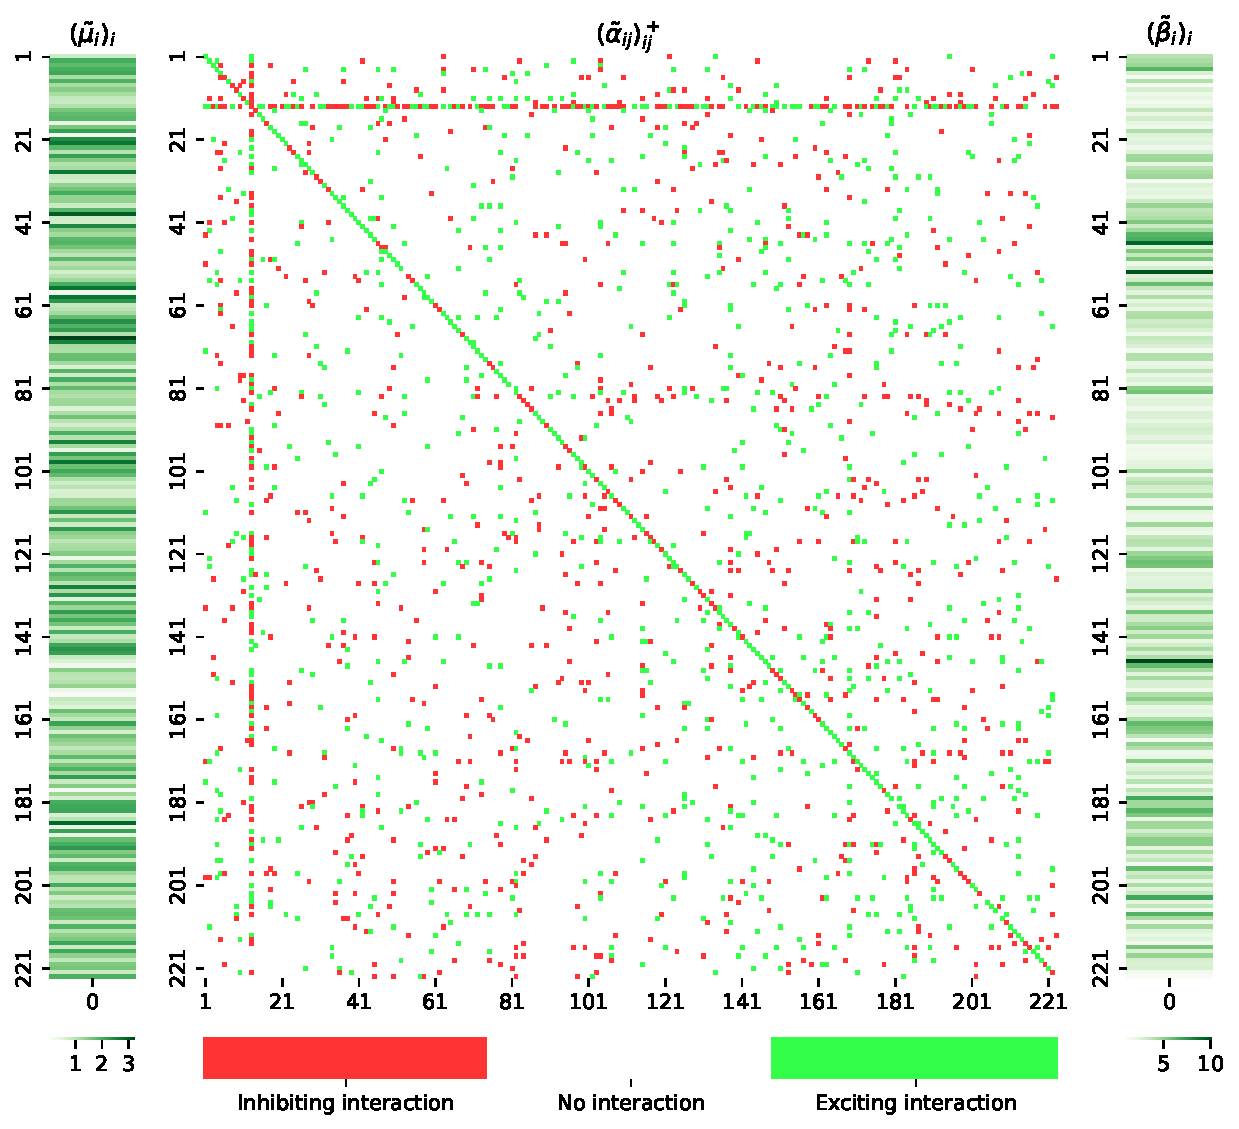
\includegraphics[width=0.8\linewidth]{images/chapter3/heatmap_mu_beta.pdf}
\caption{Heatmap $(\sign(\alpha_{ij}))_{ij}$ of (CfE) estimation on 223 neurons.}
\label{fig:chap3_heatmap_CfE}
\end{figure*}}

\section{Discussion}
\label{sec:chap3_discussion}
In this chapter, we proposed a methodology for estimating the parameters of multivariate exponential Hawkes processes with both exciting and inhibiting effects. Our first contribution was to provide a few sufficient conditions to ensure the identifiability of a commonly used model. Then we developed and implemented a maximum likelihood estimator combined with a variable selection procedure that enables to detect the significant interactions inside the whole process.
While our framework is more general than the usual linear Hawkes model, there remain two main limitations, the first one being the exponential distribution of the kernels, the second one the assumption that the delay factors \(\beta_{ij}\)
only depend on the receiving process \(N^i\). If it is essential to assume a parametric form for the kernel functions in order to maintain the concepts of our approach, it would be of great interest to consider some extensions to account for potential combined effects, as already mentioned in Section \ref{sec:chap3_comment_neuron}. It would be notably relevant to include multi-scale effects or to consider a potential lag between an event time and its actual impact.  Regarding the assumption on the delay factors, while it is quite standard, it could be a limitation of our approach when considering heterogeneous phenomena.

Going over this assumption would lead us to explore numerical integration methods and would considerably increase the computational time of the estimation procedure.
This is obviously detrimental since, in practice, time sequences are increasingly abundant and large.
On the other hand, improving the computational effectiveness of estimation procedures for Hawkes processes is a current direction of research \parencite{Bompaire2018bis}.

Our work focuses on the computational aspects of both maximum likelihood estimation and variable selection. It is of natural interest to provide further theoretical study of the asymptotic behaviour of our estimator, as done for exciting Hawkes processes \parencite{Guo2018}.
This work is currently under investigation.

Let us also highlight that, because of the physical constraints of the experiment, only a fraction of the neuronal network is observed, which raises the question of interpretability of the estimated interactions.
Indeed, the latter do not take into account the interactions with neurons that are outside the observed network.
Very recent results tackle the consistency of estimated interactions in a partially observed network \parencite{Reynaud2022}.
A necessary condition to recover interactions in the subnetwork requires in particular to have a large number of interactions within the full network.
Regarding the neuronal application, it could be of great interest to further investigate the interpretability of the inferred interactions and connectivity graph in light of the aforementioned work.


\begin{subappendices}
    \section{Proof of Lemma~\ref{lemma:chap3_restart_times}} \label{app:chap3_proof_lemma}
    In order to prove Lemma~\ref{lemma:chap3_restart_times}, let us first state a preliminary result.
    
    \begin{lemma}\label{lemma:chap3_intensity_interval_form}
        If Assumption~\ref{assu:chap3_beta} is granted, then for each $i\in\{1,\ldots, d\}$ and any $k\geq 1$:
        \begin{gather*}
            \forall t \in [T\park, T\park[k+1]),
            \\
            \lambda^{i\star}(t) = \mu_i + \left(\lambda^{i\star}(T\park\right) - \mu_i)\mathrm{e}^{-\beta_i(t-T\park)}\,.
        \end{gather*}
      \end{lemma}
  
      \begin{proof}
        Let $i\in\{1,\ldots, d\}$. For any $k\geq 1$, the underlying intensity function $\lambda^{i\star}$ in the interval $[T\park, T\park[k+1])$ can be written:
        \[\lambda^{i\star}(t) = \mu_i + \sum_{j=1}^{d}{\sum_{\ell=1}^{N^j(t)}{\alpha_{ij}\mathrm{e}^{-\beta_{ij}(t-T_\ell^j)}}}\,.\]
        This function is differentiable in the open interval $(T\park, T\park[k+1])$ and we obtain:
        \[(\lambda^{i\star})'(t) = -\sum_{j=1}^{d}{\beta_{ij}\sum_{\ell=1}^{N^j(t)}{\alpha_{ij}\mathrm{e}^{-\beta_{ij}(t-T_\ell^j)}}}\,.\]
  
        By using Assumption~\ref{assu:chap3_beta} that for all $j\in\{1,\ldots, d\}$, $\beta_{ij} = \beta_i\in\RR_+^*$, we obtain the following differential equation:
        \[(\lambda^{i\star})'(t) = -\beta_i\left(\lambda^{i\star}(t) - \mu_i\right)\,,\] which by solving on the interval gives:
        \begin{equation*}
            \lambda^{i\star}(t) = \mu_i + \left(\lambda^{i\star}(T\park) - \mu_i\right)\mathrm{e}^{-\beta_i(t-T\park)}\,.
        \end{equation*}
      \end{proof}
      
      \begin{proof}[Proof of Lemma~\ref{lemma:chap3_restart_times}]
        Let $i\in\{1,\ldots, d\}$ and $k\geq 1$.
        By Lemma~\ref{lemma:chap3_intensity_interval_form}, $\forall t \in [T\park, T\park[k+1])$:
        \begin{equation*}
            \lambda^{i\star}(t) = \mu_i + \left(\lambda^{i\star}(T\park) - \mu_i\right)\mathrm{e}^{-\beta_i(t-T\park)}\,.
        \end{equation*}
  
        In particular, the derivative of the underlying intensity function is of opposite sign as $(\lambda^{i\star}(T\park) - \mu_i)$.
        Let us distinguish two cases,
        referring to Figure~\ref{fig:chap3_lemma} for a better understanding:
        
        {\begin{figure*}[!ht]
        \centering
        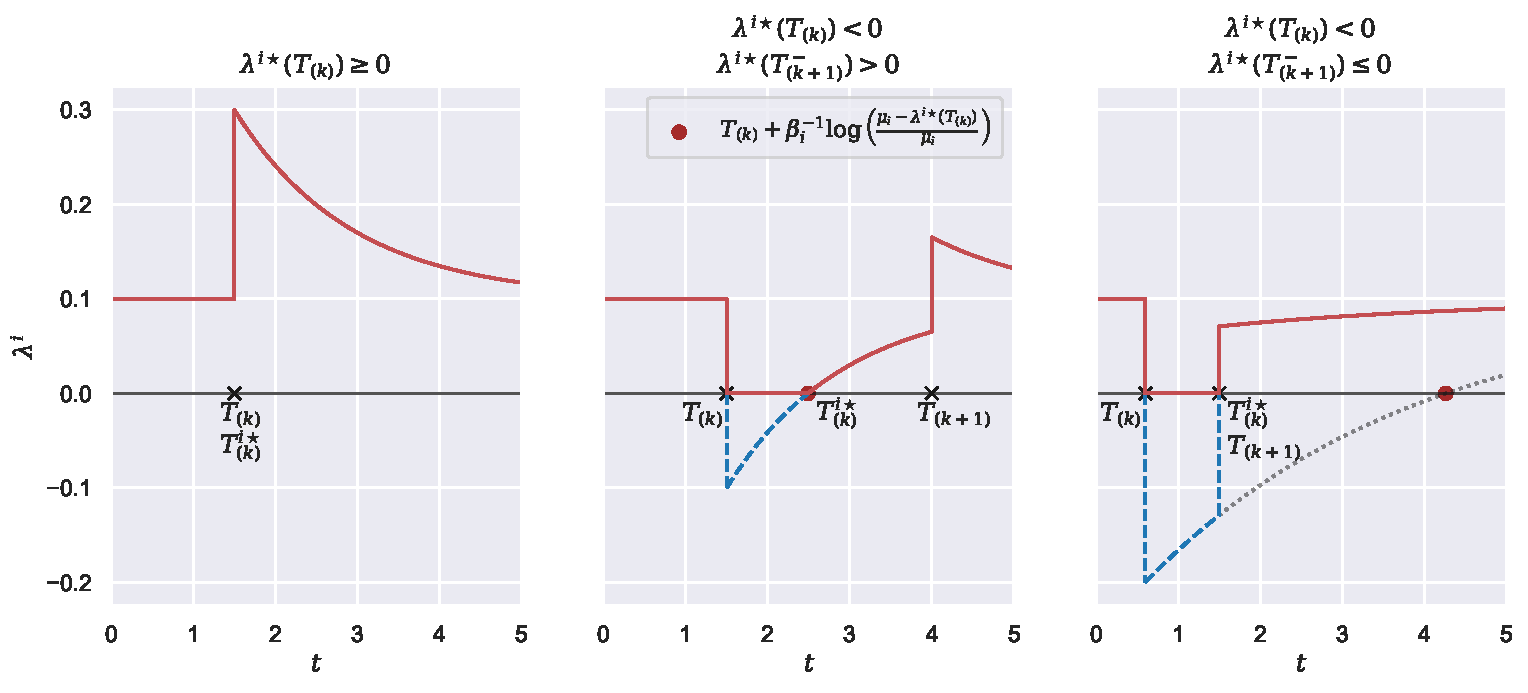
\includegraphics[width=\linewidth]{images/chapter3/cooldownTimesMarkedMulti.pdf}
        \caption{Illustration of three possible scenarios for restart times $T\park^{i\star}$ depending on the sign of $\lambda^{i\star}(T\park)$ and $\lambda^{i\star}(T\park[k+1]^-) = \lim_{t\to T\park[k+1]^-}{\lambda^{i\star}(t)}$. The dotted line in the last scenario shows the equation $\mu_i + (\lambda^{i\star}(T\park) - \mu_i)\mathrm{e}^{-\beta_i(t-T\park)} = 0$ and the term $T\park + \beta_i^{-1}\log{\adaptedpar{\frac{\mu_i - \lambda^{i\star}(T\park)}{\mu_i}}}$ as its only root.}
        \label{fig:chap3_lemma}
        \end{figure*}}
  
        \begin{itemize}
            \item If $\lambda^{i\star}(T\park) \geq 0$, then,
            \begin{align*}
              T^{i\star}\park = T\park &= \min{\adaptedpar{T\park, T\park[k+1]}} \\
              &= \min{\adaptedpar{t^\star_k, T\park[k+1]}}\,.
            \end{align*}
  
            If $(\lambda^{i\star}(T\park) - \mu_i) \geq 0$, then $\lambda^{i\star}$ is decreasing and lower-bounded by $\mu_i$. If $(\lambda^{i\star}(T\park) - \mu_i) < 0$ then $\lambda^{i\star}$ is increasing and lower-bounded by zero. In both cases, for any $t\in(T^{i\star}\park, T\park[k+1])$, $\lambda^{i\star}(t) > 0$ and then $\lambda^i(t) = \lambda^{i\star}(t)$.
  
            \item If $\lambda^{i\star}(T\park) < 0$, then $\left(\lambda^{i\star}\left(T\park\right) - \mu_i\right) < 0$ so $\lambda^{i\star}$ is strictly increasing and by continuity and by Lemma~\ref{lemma:chap3_intensity_interval_form}, there exists a unique $t^\star > T\park$ such that $\mu_i + \left(\lambda^{i\star}(T\park\right) - \mu_i)\mathrm{e}^{-\beta_i(t^\star-T\park)} = 0$.
  
                We obtain:
                \[t^\star = T\park + \beta_i^{-1}\log{\adaptedpar{\frac{\mu_i - \lambda^{i\star}(T\park)}{\mu_i}}}\,.\] By denoting $\lambda^{i\star}(T\park[k+1]^-) := \lim_{t\to T\park[k+1]^-}{\lambda^{i\star}(t)}$:
  
            \begin{itemize}
                \item If $\lambda^{i\star}(T\park[k+1]^-) > 0$, then $t^\star < T\park[k+1]$ by strict increasingness and so by definition $T^{i\star}\park = t^\star = t^\star_k$.
                Lastly, for any $t\in(T\park, T\park[k+1])$,
                if $t\in(T\park, T^{i\star}\park]$, $\lambda^{i\star}(t) \leq 0$ and then $\lambda^i(t) = 0$,
                while if $t\in(T^{i\star}\park, T\park[k+1])$, $\lambda^{i\star}(t) > 0$ and then $\lambda^i(t) = \lambda^{i\star}(t)$.
                
                \item If $\lambda^{i\star}(T\park[k+1]^-) \leq 0$, then by strict increasingness $t^\star > T\park[k+1]$ and so $T\park^{i\star} = T\park[k+1]$.
                In this case, for all $t\in(T\park, T\park[k+1])$,
                $\lambda^{i\star}(t) < 0$ so $\lambda^i(t)=0$.
                Moreover, $(T^{i\star}\park, T\park[k+1]) = \emptyset$ so we never have $\lambda^i(t) = \lambda^{i\star}(t)$.
            \end{itemize}
  
  
        \end{itemize}
  
        Combining all scenarios achieves the proof.
      \end{proof}
      
  \section{Proof of Proposition~\ref{prop:chap3_compensator}} \label{app:chap3_proof_prop_compensator}
      
      \begin{proof}
        For each $i\in\{1,\ldots, d\}$ and \(\forall t\geq 0\), with convention \(T\park[0] = 0\) and \(T\park[0]^{i\star} = 0\):
        \begin{align*}
          \Lambda^i(t)
          &= \int_{0}^{t}{\lambda^i(u)\,\mathrm{d}u}
          = \sum_{k=0}^{N(t)} \int_{T\park}^{T\park[k+1]}{\lambda^i(u) \II_{u \le t} \,\mathrm{d}u}\\
          &= \sum_{k=0}^{N(t)} \int_{T\park^{i\star}}^{T\park[k+1]} \lambda^{i\star}(u) \II_{u \le t} \, \mathrm{d}u \,,
        \end{align*}
        where the last equation comes from Lemma~\ref{lemma:chap3_restart_times}.
        Then, for \(k=0\):
        \begin{align*}
          \int_{T\park[0]^{i\star}}^{T\park[1]} \lambda^{i\star}(u) \II_{u \le t} \, \mathrm{d}u
          &= \int_{T\park[0]^{i\star}}^{T\park[1]} \mu^i \II_{u \le t} \, \mathrm{d}u\\
          &= \mu_i \min(t, T\park[1]) \,,
        \end{align*}
        and for every \(k \in \{1, \dots, N(t)\}\), by Lemma~\ref{lemma:chap3_intensity_interval_form}:
        \begin{align*}
          &\int_{T\park^{i\star}}^{T\park[k+1]} \lambda^{i\star}(u) \II_{u \le t} \, \mathrm{d}u \\
          = &\int_{T\park^{i\star}}^{T\park[k+1]} \left[ \mu_i + \left(\lambda^{i\star}(T\park\right) - \mu_i)\mathrm{e}^{-\beta_i(t-T\park)} \right] \II_{u \le t} \, \mathrm{d}u \\
          = &\mu_i \left(\min(t, T\park[k+1]) - T\park^{i\star}\right)\\ &+ \beta_i^{-1} \left(\lambda^{i\star}(T\park) - \mu_i \right) \\
          &\left(\mathrm{e}^{-\beta_i(T\park^{i\star} - T\park)} - \mathrm{e}^{-\beta_i(\min(t, T\park[k+1])- T\park)} \right)\,.
        \end{align*}
      \end{proof}
  
  \section{Proof of Theorem~\ref{th:chap3_identifiability}}\label{app:chap3_proof}
  
  \begin{proof}
      We only need to prove that if $\lambda_{\theta_i}^i(t \mid \mathcal{F}_t) = \lambda_{\theta'_i}^i(t \mid \mathcal{F}_t)$ a.e. for every $i\in\{1, \ldots, d\}$ then $\theta = \theta'$. In this proof, both intensities are considered with respect to the same filtration $\mathcal{F}_t$ so we will omit it from the rest of the proof.
      
      Let $\theta, \theta'\in \Theta$. Let us assume that $\lambda_{\theta_i}^i(t) = \lambda_{\theta'_i}^i(t)$ for all $t < T$. In order to prove equality between the two parameters we will first prove that $\mu_i = {\mu_i}'$, then $\beta_i = \beta_i'$ and lastly that $\alpha_{ij} = \alpha_{ij}'$ for every $i,j$. 
      
      \begin{itemize}
          \item For any $i$, as $\lambda_{\theta_i}^i(t) = \lambda_{\theta'_i}^i(t)$ a.e., then 
          \begin{alignat*}{2}
              &\quad& \Lambda_{\theta_i}^i(T\park[1]) &= \Lambda_{\theta'_i}(T\park[1])\\
              \implies && \mu_i T\park[1] &= {\mu_i}' T\park[1]\\
              \implies && \mu_i &= {\mu_i}'\,.
          \end{alignat*}
          
          \item For any $i$, let us choose $T\park[k+1]$ such that it is an event of process $N^i$. 
          As \[\PP(T\park[k+1] \text{ is an event of }N^i \mid \mathcal{F}_{T\park[k+1]^-}) = \frac{\lambda^i_{\theta_i}(T\park[k+1]^-)}{\lambda_{\theta}(T\park[k+1]^-)}\,,\]
          then $\lambda_{\theta_i}^i(T\park[k+1]^-) > 0$.
          By definition of $T_{(k),\theta}^{i\star}$, \[T_{(k),\theta}^{i\star} < T\park[k+1] \text{ a.s.} \,.\]
          Furthermore, $\lambda_{\theta_i}^i(t) = 0$ for $t\in(T\park, T_{(k), \theta_i}^{i\star})$ and $\lambda_{\theta_i}^i(t) > 0$ for $t\in(T_{(k), \theta_i}^{i\star}, T\park[k+1])$.
          Then, as we assumed that $\lambda_{\theta_i}^i(t) = \lambda_{\theta'_i}^i(t)$ a.e., we can conclude that $T_{(k), \theta_i}^{i\star} = T_{(k), \theta'_i}^{i\star}$. 
          By differentiating the intensity functions on the interval $(T_{(k),\theta_i}^{i\star}, T\park[k+1])$ as in the proof of Lemma \ref{lemma:chap3_restart_times} we obtain: 
          
          \begin{align*}
              \quad&(\lambda_{\theta_i}^i)'(t) = (\lambda_{\theta'_i}^i)'(t) \text{ a.e.}\\ 
              \implies &-\beta_i(\lambda_{\theta_i}^i(t) - \mu_i) =  -\beta_i'(\lambda_{\theta'_i}^i(t) - \mu_i) \text{ a.e.} \\
              \implies &(\beta_i - \beta_i')(\lambda_{\theta_i}^i(t) - \mu_i) = 0  \text{ a.s.}\\\
              \implies &\int_{T_{(k), \theta}^{i\star}}^{T\park[k+1]}{(\beta_i - \beta_i')(\lambda_{\theta_i}^i(t) - \mu_i)\,\mathrm{d}t} = 0\\
              \implies &(\beta_i - \beta_i')\int_{T_{(k), \theta}^{i\star}}^{T\park[k+1]}{(\lambda_{\theta_i}^i(t) - \mu_i)\,\mathrm{d}t} = 0\,.
          \end{align*}
          
          Additionnally,  $\lvert \lambda_{\theta_i}^i(t) - \mu_i \rvert > 0$ a.s. for all $t\in(T_{(k),\theta_i}^{i\star}, T\park[k+1])$ as $\lambda^i_{\theta_i}$ is monotone and converges to $\mu_i$. Then it follows that the integral is non-zero and so $\beta_i = \beta_i'$.        
      
      \item Let us prove the equality $\alpha_{ij} = \alpha_{ij}'$. 
      By the assumption made on the event times, for any $i,j$ with $i\neq j$, there exists two event times $\tau < \tau_+$ with $\tau$ an event time from process $N_j$ and $\tau_+$ an event time from process $N_i$ such that:
      \begin{enumerate}
          \item $\lambda_{\theta_i}^i(\tau^-) > 0$;
          \item there are only events of process $N^j$ in the interval $[\tau, \tau_+)$.
      \end{enumerate} 
      
      Let $\tau$ and $\tau_+$ be two such event times. 
      As a reminder, $T\park[N(\tau) - 1]$ corresponds to the event time before $\tau$ and similarly for $\tau_+$. 
      For $t \in [T\park[N(\tau) - 1], \tau)$, as $\lambda_{\theta_i}^i(t) = \lambda_{\theta'_i}^i(t)$ a.e.\ and by Condition \ref{hyp:chap3_ii}:
      
      \begin{equation*}
          \lambda_{\theta_i}^{i\star}(\tau^-) = \lambda_{\theta'_i}^{i\star}(\tau^-) \,.
      \end{equation*}
      
      
      By using the following equalities (proven in the previous points of the proof) 
      \begin{gather*}
      \mu_i = {\mu_i}'\,, \qquad \beta_i = \beta_i' \,,\\
      T_{(N(\tau) - 1), \theta_i}^{i\star} = T_{(N(\tau) - 1), \theta'_i}^{i\star}\,,
      \end{gather*} 
      it follows that 
      \begin{gather}
      \lambda_{\theta_i}^{i\star}(\tau^-) = \lambda_{\theta'_i}^{i\star}(\tau^-)\nonumber\\
      \implies \sum_{l=1}^{d}{\alpha_{il}\sum_{T_k^l < \tau}{\mathrm{e}^{-\beta_i(\tau - T_k^l)}}} =\sum_{l=1}^{d}{\alpha_{il}'\sum_{T_k^l < \tau}{\mathrm{e}^{-\beta_i(\tau - T_k^l)}}}\nonumber\\
      \implies \sum_{l=1}^{d}{(\alpha_{il} - \alpha_{il}')A^l}= 0\,,\label{eq:chap3_A^l}
      \end{gather}
      where \[A^l = \sum_{T_k^l < \tau}{\mathrm{e}^{-\beta_i(\tau - T_k^l)}}\,.\]
      
      We can then write Equation \eqref{eq:chap3_A^l} by replacing $\tau$ by $\tau_+$ as $\lambda_{\theta_i}^i(\tau_+^-) > 0$ because $\tau_+$ is an event time of process $N^i$.  We obtain then
      \begin{equation}\label{eq:chap3_B^l}
          \sum_{l=1}^{d}{(\alpha_{il} - \alpha_{il}')B^l} = 0\,,
      \end{equation}
      where \[B^l = \sum_{T_k^l < \tau_+}{\mathrm{e}^{-\beta_i(\tau_+ - T_k^l)}}\,.\]
      
     By definition of event times $\tau$ and $\tau_+$, all events on the interval $[\tau, \tau_+)$ are from process $N^j$ so we obtain for all $l \neq j$, \[B^l = A^l \mathrm{e}^{-\beta_i(\tau_+ - \tau)}\,.\] 
      For $l=j$, 
      \[B^j = A^j\mathrm{e}^{-\beta_i(\tau_+ - \tau)} + \sum_{\tau \leq T_k^j < \tau_+}{\mathrm{e}^{-\beta_i(\tau_+ - T_k^j)}}\,,\] 
      where the second term of the right hand side is positive as interval $[\tau, \tau_+)$ contains at least one event, $\tau$, from process $N^j$. 
      We can rewrite then Equation \eqref{eq:chap3_B^l}:
      \begin{equation*}
      \sum_{l=1}^{d}{(\alpha_{il} - \alpha_{il}')B^l} = 0
      \end{equation*}
      \begin{align*}
      \implies &\mathrm{e}^{-\beta_i(\tau_+ - \tau)}\sum_{l=1}^{d}{(\alpha_{il} - \alpha_{il}')A^l} \\
      &+ (\alpha_{ij}-\alpha_{ij}')\sum_{\tau \leq T_k^j < \tau_+}{\mathrm{e}^{-\beta_i(\tau_+ - T_k^j)}} = 0\,.
      \end{align*}
          
      By Equation \eqref{eq:chap3_A^l}, the first term is null and the second sum is non-zero as interval $[\tau, \tau_+)$ contains at least an event from process $N^j$. It follows that:
      
      \begin{gather*}
          (\alpha_{ij}-\alpha_{ij}')\sum_{\tau \leq T_k^j < \tau_+}{\mathrm{e}^{-\beta_i(\tau_+ - T_k^j)}} = 0\\
          \implies \quad (\alpha_{ij}-\alpha_{ij}') = 0\,.
      \end{gather*}
      
      It follows that for every $j\neq i$, $\alpha_{ij}=\alpha_{ij}'$. It remains to prove that $\alpha_{ii}=\alpha_{ii}'$. For this, let $T^i_2$ be the second event time of process $N^i$. We can the write the equality 
      
          \begin{equation*}
          \lambda_{\theta_i}^{i\star}(T_2^i) - \lambda_{\theta'_i}^{i\star}(T^i_2) = 0 \,,
      \end{equation*}
      \begin{equation*}
           \implies \sum_{l=1}^{d}{(\alpha_{il} - \alpha'_{il}) \sum_{T_k^l < T^i_2}{\mathrm{e}^{-\beta_i(\tau - T_k^l)}}}= 0 \,,
      \end{equation*}
      \begin{equation*}
           \implies (\alpha_{ii} - \alpha'_{ii}) \sum_{T_k^i < T^i_2}{\mathrm{e}^{-\beta_i(\tau - T_k^l)}}= 0 \,,
      \end{equation*}
      as for $j\neq i$, $\alpha_{ij}=\alpha_{ij}'$. The sum is non-zero as it contains the event $T^i_1$ and so we obtain $\alpha_{ii}=\alpha_{ii}'$. 
  
  \end{itemize}
  This achieves the proof.
  \end{proof}
  
  \section{Proof of Corollary~\ref{cor:chap3_mle}} \label{app:chap3_proof_cor_mle}
      \begin{proof}
            For all \(i \in \{1, \dots, d\}\), \(\theta \in \Theta\) and \(k \in \mathbb N^*\),
            \begin{align*}
              \log{\lambda^i_{\theta_i}(T_k^{i-})}
              = &- \infty \II_{\lambda^i_{\theta_i}(T_k^{i-}) = 0} \\
              &+ \log{\lambda^i_{\theta_i}(T_k^{i-})} \II_{\lambda^i_{\theta_i}(T_k^{i-}) > 0} \\
              = &- \infty \II_{\lambda^{i\star}_{\theta_i}(T_k^{i-}) \le 0} \\
              &+ \log{\lambda^{i^\star}_{\theta_i}(T_k^{i-})} \II_{\lambda^{i\star}_{\theta_i}(T_k^{i-}) > 0} \\
              = &\log{\lambda^{i^\star}_{\theta_i}(T_k^{i-})} \\
              = &\log{\lim_{t \to T_k^{i-}} \lambda^{i^\star}_{\theta_i}(t)}.
            \end{align*}
            Now, for \(k=1\), \(\lambda^{i^\star}_{\theta_i}(T_k^{i-}) = \mu_i\),
            and for \(k \geq 2\), let us note \(q = N(T_k^i)-1\).
            Then,
            \[
              [T\park[q], T\park[q+1]) = [T\park[N(T_k^i)-1], T\park[N(T_k^i)]) = [S_k^i, T_k^i) \,,
            \]
            and by Lemma~\ref{lemma:chap3_intensity_interval_form}, \(\forall t \in [T\park[q], T\park[q+1])\):
            \begin{align*}
              \lambda_\theta^{i\star}(t)
              &= \mu_i + \left(\lambda_{\theta_i}^{i\star}(T\park[q]) - \mu_i\right)\mathrm{e}^{-\beta_i(t-T\park[q])}\\
              &= \mu_i + \left(\lambda_{\theta_i}^{i\star}(S_k^i) - \mu_i\right)\mathrm{e}^{-\beta_i(t-S_k^i)}\,.
            \end{align*}
            Thus, 
            \begin{align*}
              \lim_{t \to T_k^{i-}} \lambda^{i^\star}_{\theta_i}(t)
              &= \lim_{t \to T\park[q]^{-}} \lambda^{i^\star}_{\theta_i}(t)\\
              &= \mu_i + \left(\lambda_{\theta_i}^{i\star}(S_k^i) - \mu_i\right)\mathrm{e}^{-\beta_i(T_k^{i}-S_k^i)}\,.
            \end{align*}
            To conclude, by Equation~\eqref{eq:chap3_general_log_likelihood},
            \begin{align*}
              \ell_t^{i}(\theta_i)
              = &\sum_{k=1}^{N^i(t)}{\log{\lambda^i_{\theta_i}(T_k^{i-})}} - \Lambda_{\theta_i}^i(t) \\
              = &\log{\lambda^i_{\theta_i}(T_1^{i-})} + \sum_{k=2}^{N^i(t)}{\log{\lambda^i_{\theta_i}(T_k^{i-})}} - \Lambda_{\theta_i}^i(t) \\
              = &\log{\mu_i} + \sum_{k=2}^{N^i(t)}{\log \left(\mu_i + \left(\lambda_{\theta_i}^{i\star}(S_k^i) - \mu_i\right)\mathrm{e}^{-\beta_i(T_k^{i}-S_k^i)} \right)}\\
              &- \Lambda_{\theta_i}^i(t) \,.
            \end{align*}
      \end{proof}
  
  
  \section{Algorithm for computing the log-likelihood}
  \label{app:chap3_log-lik}
  
  This section presents Algorithm \ref{alg:chap3_likelihood} for computing the log-likelihood $\ell_t(\theta)$ by leveraging the results from Corollary \ref{cor:chap3_mle}.
    \begin{algorithm}[!ht]
    \SetAlgoLined
     \textbf{Input} Parameters $\mu_i$, $\alpha_{ij}$, $\beta_i$ for $i,j\in\{1,\ldots, d\}$, list of event times and marks $(T\park, m_k)_{k=1:N(t)}$\;
     \textbf{\underline{Initialisation}} Initialise for all $i$, $\Lambda^i_k = \mu_i T\park[1]$, $\lambda^{i\star}(T\park^-) = \mu_i$, $\lambda_k^{i\star} = \mu_i + \alpha_{im_1}$ and $\ell_t(\theta) = \log(\lambda^{m_1\star}(T\park^-)) - \sum_{i=1}^{d}{\Lambda^i_k}$\;
     \For{$k = 2 \text{ to } N(t)$}{
  
     Compute for all $i$, $T\park[k-1]^{i\star} = \min{\adaptedpar{T\park[k-1] + \beta_i^{-1}\log{\adaptedpar{\frac{\mu_i - \lambda_k^{i\star}}{\mu_i}}}\II_{\{\lambda_k^{i\star} < 0\}}, T\park}}$\;
  
     Compute for all $i$, $\Lambda^i_k = \mu_i(T\park - T\park[k-1]^{i\star}) + \beta_i^{-1}(\lambda_k^{i\star} - \mu_i)(\mathrm{e}^{-\beta_i(T\park[k-1]^{i\star} - T\park[k-1])} - \mathrm{e}^{-\beta_i(T\park- T\park[k-1])})$\;
  
     Compute for all $i$, $\lambda^{i\star}(T\park^-) = \mu_i + (\lambda^{i\star}_k - \mu_i)\mathrm{e}^{-\beta_i(T\park - T\park[k-1])}$\;
  
     Update $\ell_t(\theta) = \ell_t(\theta) + \log(\lambda^{m_k\star}(T\park^-)) - \sum_{i=1}^{d}{\Lambda^i_k}$\;
  
     Compute for all $i$, $\lambda_k^{i\star} = \lambda^{i\star}(T\park^-) + \alpha_{im_k}$\;
  
     }
     Compute for all $i$, $T\park[N(t)]^{i\star} = \min{\adaptedpar{T\park[N(t)] + \beta_i^{-1}\log{\adaptedpar{\frac{\mu_i - \lambda_k^{i\star}}{\mu_i}}}\II_{\{\lambda_k^{i\star} < 0\}}, t}}$\;
  
     Compute for all $i$, $\Lambda^i_k = \left[\mu_i(t - T\park[N(t)]^{i\star}) + \beta_i^{-1}(\lambda_k^{i\star} - \mu_i)(\mathrm{e}^{-\beta_i(T_{N(t)}^{i\star} - T\park[N(t)])} - \mathrm{e}^{-\beta_i(t- T\park[N(t)])})\right]\II_{\{t > T\park[N(t)]^{i\star}\}}$\;
  
     Update $\ell_t(\theta) =  \ell_t(\theta) - \sum_{i=1}^{d}{\Lambda^i_k}$\;
  
     \Return Log-likelihood $\ell_t(\theta)$.
     \caption{Computation of the log-likelihood $\ell_t(\theta)$ of a multivariate exponential Hawkes process.}
     \label{alg:chap3_likelihood}
    \end{algorithm}
  
  
  \section{Reconstructed interaction functions for synthetic data}
  \label{app:chap3_numerical}
  
  This section presents the reconstruction of interaction functions $h_{ij}$ along with the estimated functions $\tilde h_{ij}$ from the two-dimensional Hawkes processes simulations as described in Section \ref{sec:chap3_dim2}. Figure \ref{fig_supp:scenario_1} and Figure \ref{fig_supp:scenario_2} correspond respectively to the estimations for Scenarios (1) and (2) from Table \ref{tab:chap3_simulated_2_table}.
  
  {\begin{figure}[!ht]
       \centering
       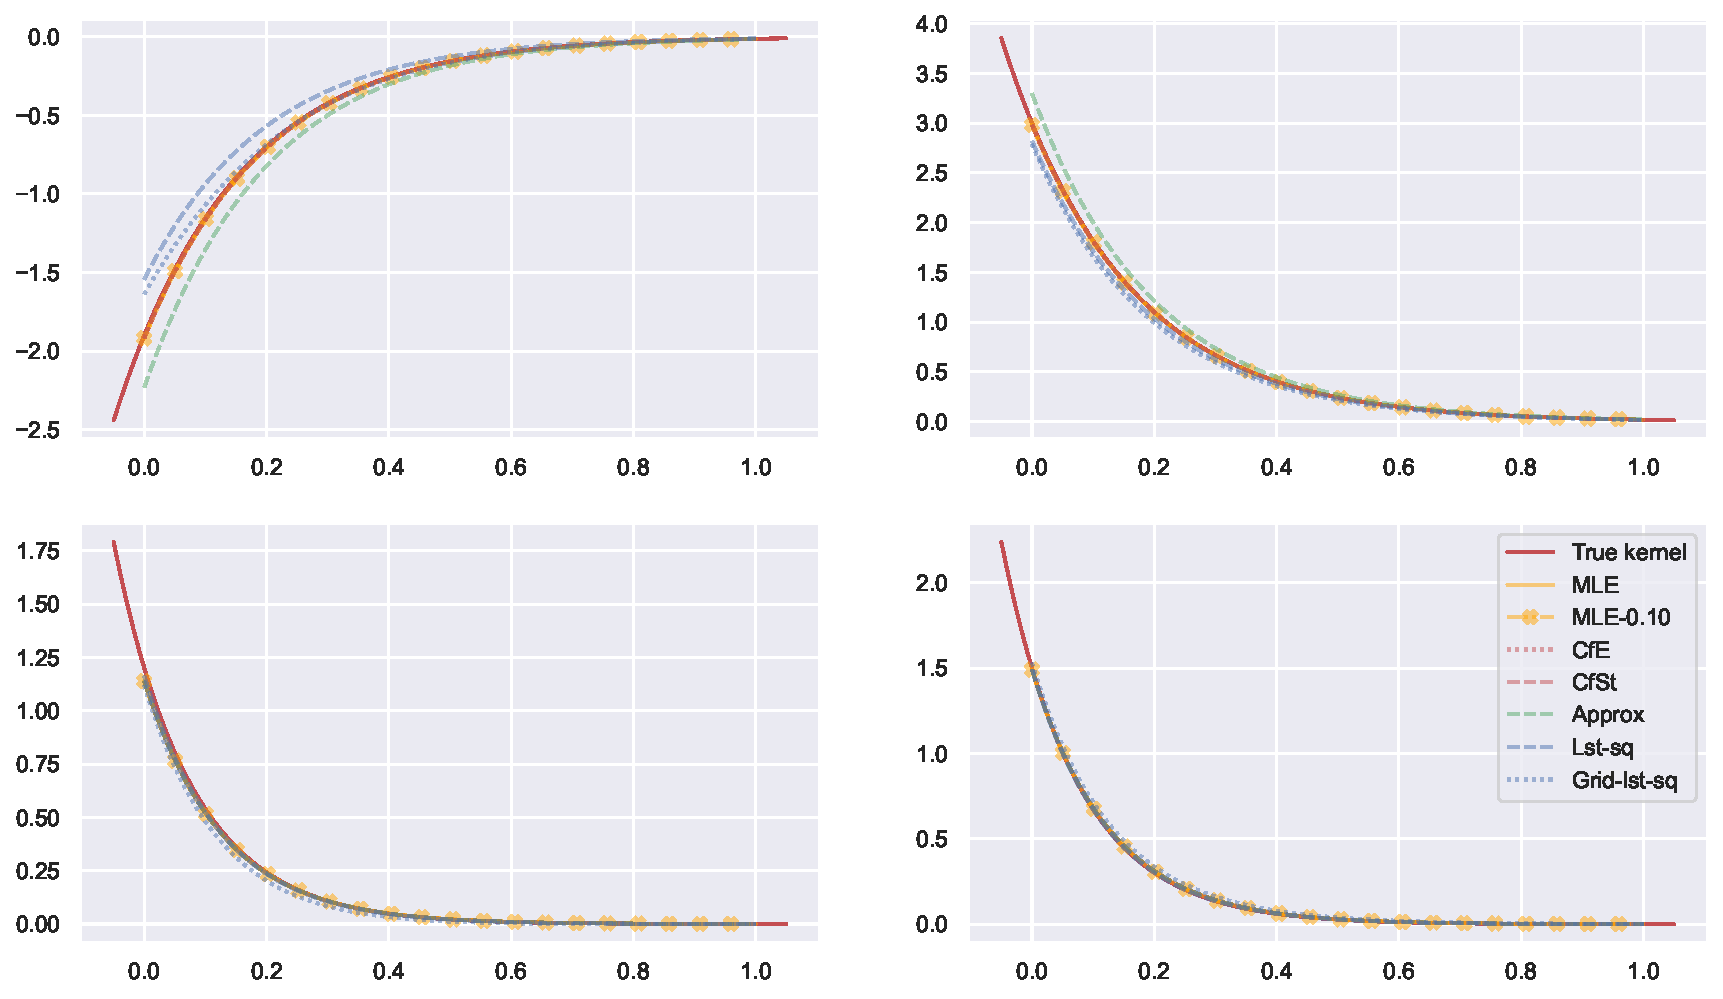
\includegraphics[width=\linewidth]{images/chapter3/reconstruction_param_1.pdf}
       \caption{Reconstruction of interaction functions $h_{ij}$ for Scenario (1) of two-dimensional Hawkes processes along with all estimated functions $\tilde h_{ij}$. The real function is plotted in red and 25 estimations are averaged for each method.}
       \label{fig_supp:scenario_1}
       \end{figure}}
       
  {\begin{figure}[!ht]
       \centering
       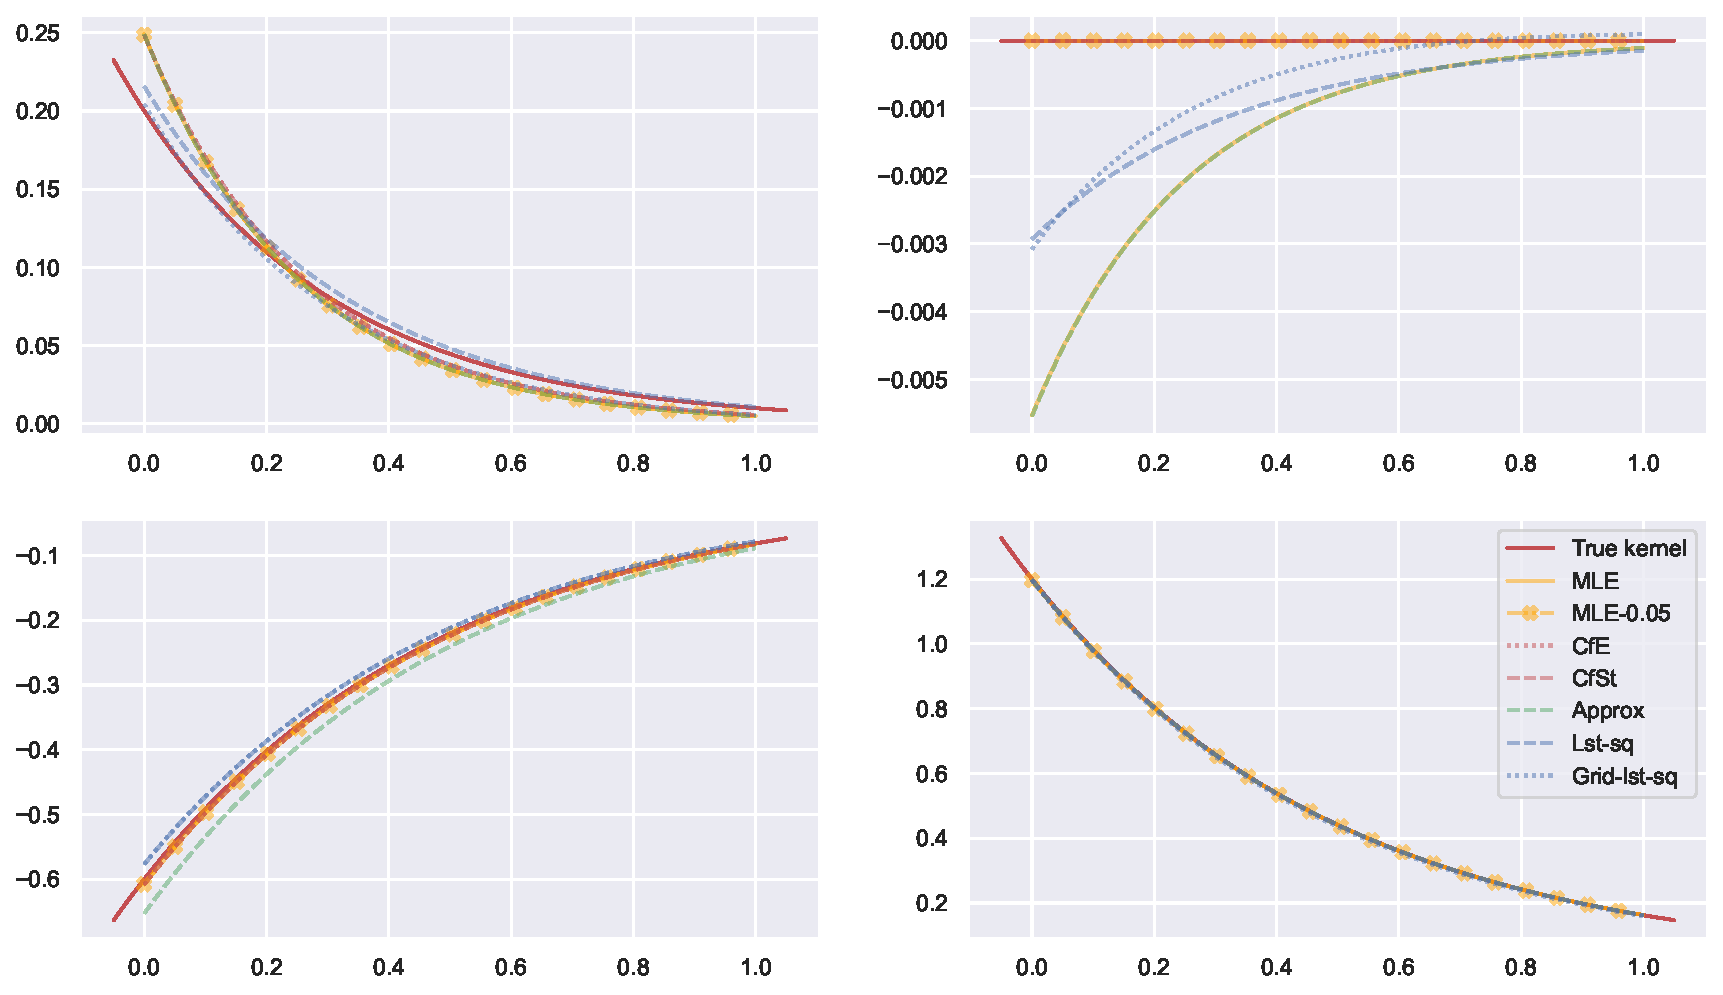
\includegraphics[width=\linewidth]{images/chapter3/reconstruction_param_2.pdf}
       \caption{Reconstruction of interaction functions $h_{ij}$ for Scenario (2) of two-dimensional Hawkes processes along with all estimated functions $\tilde h_{ij}$. The real function is plotted in red and 25 estimations are averaged for each method.}
       \label{fig_supp:scenario_2}
       \end{figure}}
\end{subappendices}
\leadchapter{
    Classic estimation methods for Hawkes processes rely on the assumption that observed event times are indeed a realisation of a Hawkes process,
    without considering any potential perturbation of the model.
    However, in practice, observations are often altered by some noise, the form of which depends on the context.
    It is then required to model the alteration mechanism in order to infer accurately such a noisy Hawkes process.
    While several models exist,
    we consider, in this work, the observations to be the indistinguishable union of event times coming from a Hawkes process and from an independent Poisson process. 
    Since standard inference methods (such as maximum likelihood or Expectation-Maximisation) are either unworkable or numerically prohibitive in this context,
    we propose an estimation procedure based on the spectral analysis of second order properties of the noisy Hawkes process.
    Novel results include
    sufficient conditions for identifiability of the ensuing statistical model with exponential interaction functions for both univariate and bivariate processes. Although we mainly focus on the exponential scenario, other types of kernels are investigated and discussed.
    A new estimator based on maximising the spectral log-likelihood is then described,
    and its behaviour is numerically illustrated on synthetic data.
    Besides being free from knowing the source of each observed time (Hawkes or Poisson process),
    the proposed estimator is shown to perform accurately in estimating both processes.
}
\chapter[][]{Spectral analysis for the  inference of noisy Hawkes processes}

% sec, fig, eq, tab, def, prop, cor, hyp, rem, 


\section{Introduction}
     
       Hawkes processes, introduced in \textcite{Hawkes1971}, are a class of point processes that have been originally used to model self-exciting phenomena and more recently other types of past-dependent behaviours.
   Their fields of applications are wide and include for instance seismology \parencite{Ogata1988, Ogata1998}, neuroscience \parencite{Chornoboy1988, Lambert2018}, criminology \parencite{Olinde2020}, finance \parencite{Embrechts2011, Bacry2015} and biology \parencite{Gupta2018}, to mention a few.
         Consequently, there has been a deep focus on estimation techniques for Hawkes processes. Among them, let us mention maximum likelihood approaches \parencite{Ogata1978, Ozaki1979, Guo2018}, methods of moments \parencite{DaFonseca2013}, least-squares contrast minimisation \parencite{Reynaud2014,Bacry2020}, Expectation-Maximisation (EM) procedures \parencite{Lewis2011}, and methods using approximations through autoregressive models \parencite{Kirchner2017}.
        
        All of these methods are based on the assumption that the history of the process has been accurately observed, although this information is partial or noised in many contexts, in particular due to measurement or detection errors.
        Different models, described notably in \textcite{Lund2000}, have been proposed to handle such errors for spatial point processes, with inference methods based on approximating the likelihood depending on each noise scenario.
            The first scenario, called \textit{displacement}, is when the event times are observed with a shift. If deconvolution methods to recover the unnoised process are standard approaches for simpler point processes such as Poisson processes (see for instance \textcite{Antoniadis2006,Bonnet2022} or the review by \textcite{Hohage2016}), the literature for Hawkes processes remains scarce and consists of the work of \textcite{Trouleau2019} where the event times are observed with a delay and the work of \textcite{Deutsch2020} where the shift follows a Gaussian distribution. The latter also explores the framework where some event times are undetected, which is similar to that studied in \textcite{Mei2019}. This setting can either be referred to as \textit{thinning} when the observations are randomly missing, or \textit{censoring} when complete regions are unobserved. The last scenario, called \textit{Superposition of ghost points} by \textcite{Lund2000}, is the focus of this paper and describes situations where additional points are coming from an external point process, in our case a Poisson process.   A real-world application that motivated this work comes from spike trains analysis in neuroscience: the membrane potential, which is a continuous signal, is recorded and when it exceeds a certain threshold, one considers that an event time, called a spike, occurred. However, since the original signal is noised, it is possible to detect spikes that do not correspond to real events.
          Regarding inference of such a noisy process, let us highlight that exact likelihood approaches are intractable due to the unknown origin of each occurrence (Hawkes process or noise process) while methods based on inferring this missing information, for instance Expectation-Maximisation algorithms, are computationally too demanding.
               
               Inspired by the work of \textcite{Cheysson2022} when the event times of a Hawkes process are aggregated, we turn to spectral analysis (Section~\ref{sec:chap3_spectral_analysis}) to propose a novel estimation procedure that allows to infer the noisy Hawkes process.
               On the way, we present a general characterisation of the Bartlett spectrum of the superposition of two independent processes (Section~\ref{sec:chap3_superposition})
               and identifiability results of the statistical model in the univariate (Section~\ref{sec:chap3_univariate_noisy_hawkes}) and the bivariate (Section~\ref{sec:chap3_dim2}) settings.
               Inference in these two settings is numerically illustrated in Section~\ref{sec:chap3_numerical_results}.
               Before starting, we present the mathematical setting (Section~\ref{sec:chap3_setting})
               and review the references related to spectral approaches (Section~\ref{sec:chap3_related_works}).


    
      \subsection{Mathematical setting}
      \label{sec:chap3_setting}
        Let $H = (H_1, \ldots, H_d)$ be a stationary multivariate Hawkes process on $\RR$ defined by its conditional intensity functions $\lambda_i^H$ ($i \in \{1, \dots, d\}$):
        for all $t \in \RR$,
        \begin{equation}\label{eq:chap3_hawkes_intensity}
          \lambda_i^H(t) = \mu_i + \sum_{j=1}^{d}\int_{-\infty}^{t}{h_{ij}(t-s) \, H_j(\dd s)} = \mu_i + \sum_{j=1}^{d}\sum_{T^{H_j}_k \leq t}{h_{ij}(t  - T_k^{H_j})}\,,
        \end{equation}
        where $\mu_i > 0$ is the baseline intensity of process $H_i$,
        $h_{ij} : \RR \to \RR_{\ge 0}$ is the interaction or kernel function describing the effect of process $H_j$ on process $H_i$,
        and $(T_k^{H_j})_{k\ge1}$ denotes the event times of $H_j$.
        
        By defining the matrix $S = (\|h_{ij}\|_1)_{1 \le i, j \le d}$,
        where
        \[\|h_{ij}\|_1 = \int_{-\infty}^{+\infty}{h_{ij}(t) \, \dd t}\,,\]
        the stationarity condition of $H$ reduces to controlling the spectral radius of $S$: $\rho(S)<1$ \parencite{Bremaud1996}. 
        
        The goal of this paper is to study a noisy version of the Hawkes process where the sequences of event times $(T_k^{H_1})_{k\ge1}$, \dots, $(T_k^{H_d})_{k\ge1}$ of $H$ are contaminated by the event times from another process $P$.
        Since the latter process is aimed at modeling an external noise mechanism due to errors in the detection of event times,
        it is naturally assumed that each subprocess of $H$ is perturbed uniformly with the same level of noise,
        such that $P$ is chosen to be a multivariate Poisson process with same intensity across subprocesses.
        Formally, let $P = (P_1, \ldots, P_d)$ be a multivariate homogeneous Poisson process on $\RR$, supposed to be independent from $H$, where each univariate process $P_i$ has the same intensity $\lambda_0 > 0$.
        We note the event times $(T_k^{P_i})_{k\ge1}$ ($i \in \{1, \dots, d\}$).        
        We consider then the point process $N = (N_1, \ldots, N_d)$ defined as the superposition of $H$ and $P$ (Definition~\ref{def:chap3_superposition}):
        the sequence of event times $(T_k^{N_i})_{k\ge1}$ of $N_i$ ($i \in \{1, \dots, d\}$) is the ordered union of $(T_k^{H_i})_{k\ge1}$ and $(T_k^{P_i})_{k\ge1}$.
        
        Throughout this paper we will refer to $N$ as the noisy Hawkes process,
        and it will be assumed that event times of $N$ are observed without knowing their origin (Hawkes or Poisson process).
        Our goal is to estimate both processes (\ie the baselines $\mu_i$, the kernels $h_{ij}$ and the shared Poisson intensity $\lambda_0$) from the sole observation of $(T_k^{N_i})_{k\geq1}$, $i \in \{1, \dots, d\}$.
        
        Inference procedures for point processes often leverage the intensity functions in order to devise maximum likelihood and method of moment estimators \parencite{Ogata1988, Ozaki1979, DaFonseca2013}.
        Here, the process of interest $N$ being a superposition of two independent point processes,
        the intensity of each subprocess $N_i$ reads (for any integer $i \in \{1, \dots, d\}$):
        for all $t \in \RR$,
        \begin{equation}
          \lambda_i^N(t) = \lambda_0 + \mu_i + \sum_{j=1}^{d}\int_{-\infty}^{t}{h_{ij}(t-s) \, H_j(\dd s)}\,.
          \label{eq:chap3_intensity_noisy}
        \end{equation}
        However, it appears from Equation~\eqref{eq:chap3_intensity_noisy} that usual estimators cannot be designed from intensity functions $\lambda_1^N, \dots, \lambda_d^N$ since they are based on $H$, 
        which is indistinguishable from $P$ in our setting.
        
        In order to estimate the Hawkes and the Poisson components of $N$,
        we propose to leverage the spectral analysis of point processes,
        recently advocated by \textcite{Cheysson2022} for inference of aggregated Hawkes processes.        
        It consists in considering, for a multivariate point process, its matrix-valued spectral density function, denoted $\mathbf f : \RR \to \mathbb C^{d \times d}$,
        which is related to second-order measures \parencite{Bartlett1963}.
        Given some observed
        times $(T_k^{N_1})_{k\ge1}$, \dots, $(T_k^{N_d})_{k\ge1}$,
        (in a prescribed time window $[0, T]$),
        the spectral density is linked to cross-periodograms,
        defined for all pairs $(i, j) \in \{1, \dots, d\}^2$ and all $\omega \in \RR$ by:
        \begin{equation}\label{eq:chap3_multivariate_periodogram}
          I_{ij}^T(\omega) = \frac{1}{T}\sum_{k=1}^{N_i(T)}\sum_{l=1}^{N_j(T)}\mathrm{e}^{-2 \pi \iu \omega (T_k^{N_i} - T_l^{N_j})}\,,
        \end{equation}
        where $N_i(t) = N_i([0, t))$.
        Indeed, considering the matrix-valued function $\mathbf I^T : \omega \in \RR \mapsto (I_{ij}^T(\omega))_{1 \le i, j \le d}$,
        the aforementioned link is to be understood as $\mathbf I^T(\omega)$ (for all $\omega \in\RR$) being asymptotically distributed according to a complex Wishart distribution with one degree of freedom and scale matrix $\mathbf f(\omega)$ \parencite{Tuan1981, Villani2022}.
        In particular, this implies that \(\mathbb E [\mathbf I^T(\omega)] = \mathbf f(\omega)\).
        Moreover, it is noteworthy that the periodogram $\mathbf I^T(\omega)$ can be computed regardless of knowing the source of the event times.
        This paves the way for estimation.
        
        As it happens, in the scope of statistical inference, a parametric model for the matrix-valued spectral density function is considered:
        \[
            \mathcal{P} = \left\{
              \mathbf{f}_\theta^N : \RR \to \mathbb C^{d \times d},
              \theta = (\mu, \gamma, \lambda_0)\in \Theta
            \right\} \,,
        \]
        where $\gamma$ is a parameter that characterises the interaction functions.
        Then, for $\omega_k = k/T$ ($k \in \{1, 2, \dots\}$), it can be shown that $(\mathbf I^T(\omega_k))_{k \geq 1}$ are asymptotically independent,
        leading to the approximate spectral log-likelihood \parencite{Brillinger2012, Duker2019, Villani2022}:
        \begin{equation}\label{eq:chap3_spectral_log_likelihood}
	        \ell_T(\theta) = -\frac{1}{T} \sum_{k=1}^{M}
	        \Big\{
	          \log\left(\det\left(\mathbf{f}_\theta^N(\omega_k)\right)\right) +
	          \Tr\left(\mathbf{f}_\theta^N(\omega_k)^{-1}\mathbf{I}^T(\omega_k)\right)
	        \Big\} \,,
        \end{equation}
        where $\det$ and $\Tr$ are respectively the determinant and trace of matrices.
        Then, the so-called Whittle (or spectral) estimator $\mathbf f_{\hat \theta}^N$ of $\mathbf f$ \parencite{Whittle1952} is obtained for \(\hat \theta \in \Theta\) such that
        \[
          \hat \theta \in \arg\max_{\theta \in \Theta}~ \ell_T (\theta) \,.
        \]
         
        
        

      \subsection{Related works}
      \label{sec:chap3_related_works}
        The spectral analysis of point processes was introduced in \textcite{Bartlett1963} and extended to 2-dimensional point processes in \textcite{Bartlett1964}.
        Subsequent research works focusing on the theoretical properties of the Bartlett spectrum include \textcite{Daley1971, DaleyV1, Tuan1981} for temporal settings and \textcite{Mugglestone1996, Mugglestone2001, Rajala2023} for spatial contexts.
        
        Despite this, practical applications remain scarcer in the literature.
        \textcite{Adamopoulos1976} studies earthquake arrivals through the analysis of Hawkes processes and \textcite{Karavasilis2007} analyses the cross-correlation of bivariate point processes in the context of muscular stimulation.
        
        In a recent contribution by \textcite{Cheysson2022}, the authors employ the spectral analysis of point processes to infer an aggregated Hawkes process. More precisely, the observations are assumed to come from a standard Hawkes process but only the counts of events on fixed intervals are available.
        By leveraging the properties of the Bartlett spectrum, they propose an estimator obtained by means of maximisation of the spectral log-likelihood.

        The main advantage of the spectral approach is its obvious ability to handle different kinds of partial observations.
        That is why we propose an inference procedure for noisy Hawkes processes based on Bartlett's spectral density.
        
        Spectral results concerning the Hawkes model are built on the linearity of the intensity function along with its branching properties.
        The first spectral analysis of linear Hawkes processes appears in the original paper \textcite{Hawkes1971} and was then developed in \textcite{DaleyV1} in both univariate and multivariate contexts.
        Explicit expressions of the spectral density of a Hawkes process are available as long as the Fourier transform of the kernel functions are known, which allows to work with a wide array of parametrisations.

        In this paper, we mainly focus on studying identifiability of the statistical model with the classic exponential kernel
        (and also give insights about identifiability with other kernels).
        We subsequently derive a parametric inference procedure for estimating the parameters of a process composed of the superposition of a linear Hawkes process and a homogeneous Poisson process.

        
    \section{Spectral analysis}\label{sec:chap3_spectral_estimation}
      \subsection{The Bartlett spectrum}\label{sec:chap3_spectral_analysis}
        In this section, we formally introduce the concept of matrix-valued spectral measure
        $\mathbf \Gamma : \RR \to \mathbb C^{d \times d}$
        for a multivariate stationary point process $N = (N_1, \ldots, N_d)$.
        This is an extension of the Bartlett spectrum introduced by \textcite{Bartlett1963} for the analysis of univariate point processes.
        Let $\mathcal S$ be
        the space of real functions on $\RR$ with rapid decay \parencite[Chapter 8.6.1]{DaleyV1}:
        \[
          \mathcal S = \left\{ f \in C^\infty, \forall k \in \{1, 2, \dots\}, \forall r \in \{1, 2, \dots\},
          \sup_{x \in \RR} \left| x^r
          f^{(k)}(x)
          \right| < \infty \right\},
        \]
        where $C^\infty$ is the set of smooth functions from $\RR$ to $\RR$
        and $f^{(k)}$ is the \(k^\text{th}\) derivative of \(f \in C^\infty\).

        Then, the Bartlett spectrum of $N$ is the
        matrix-valued function $\mathbf{\Gamma}^N : \omega \in \RR \mapsto (\Gamma_{ij}^N(\omega))_{1 \le i, j \le d} \in \mathbb C^{d \times d}$, such that for all $1 \le i,j \le d$, $\Gamma_{ij}^N$ is a measure on $\RR$ verifying \parencite[Equation 8.4.13]{DaleyV1}:
        \[
          \forall (\varphi, \psi) \in \mathcal S \times \mathcal S:
          \quad
          \Cov \left(
            \int_{\RR}{\varphi(x) \, N_i(\mathrm{d}x)} , \int_{\RR}{\psi(x) \, N_j(\mathrm{d}x)}
          \right)
          = \int_{\RR}{ \tilde{\varphi} (\omega) \tilde{\psi}(-\omega) \, \Gamma_{ij}^N (\mathrm{d}\omega)}\,,
        \]        
        where for all $f \in \mathcal S$, $\tilde f : \RR \to \mathbb C$ denotes the Fourier transform of $f$:
        \[
          \forall \omega \in \RR: \quad
          \tilde f(\omega) = \int_{\RR}{ f(x) \mathrm{e}^{-2\pi \iu x \omega} \, \dd x} \,.
        \]
        
        If, for all $1 \le i, j \le d$, the measure $\Gamma_{ij}^N$ is absolutely continuous,
        we can define the matrix-valued spectral density function of $N$, denoted $\mathbf f^N : \RR \to \mathbb C^{d \times d}$,
        such that for all $\omega \in \RR$, $\mathbf f^N(\omega) = (f^N_{ij}(\omega))_{1 \le i, j \le d}$
        with \(\Gamma_{ij}^N(\dd \omega) = f_{ij}^N(\omega) \, \dd \omega\).
      	
      	From a practical point of view, the spectral density $\mathbf f^N$ can be derived from the reduced covariance densities. 
        Let $\mathcal{B}_{\RR}^c$ be the collection of all bounded Borel sets on \(\RR\) and $\ell_{\RR} : \mathcal B_{\RR}^c \to \RR_{\ge0}$ the Lebesgue measure on \(\RR\).
        For all $i \in \{1, \dots, d\}$, the first moment measure of process $N_i$ is defined as $A \in \mathcal B_\RR^c \mapsto \EE[N_i(A)]$ and, by stationarity of the process,
        it comes:
        \[\forall A\in\mathcal{B}_{\RR}^c: \quad \EE[N_i(A)] = m_i^N \ell_{\RR}(A)\,,\]
        where $m_i^N = \EE[N_i([0, 1))]$ is the mean intensity of process $N_i$.
        Then, for all \((i, j) \in \{1, \dots, d\}^2\) the second order moment measure $M_{ij}^N : \mathcal B_\RR^c \times \mathcal B_\RR^c \to \RR_{\ge0}$ is defined by \parencite[Section~5.4]{DaleyV1}:
        \[
          \forall (A, B) \in \mathcal{B}_{\RR}^c \times \mathcal{B}_{\RR}^c: \quad
    	    M_{ij}^N(A, B) = \EE[N_i(A)N_j(B)] = \int_{A\times B}{M_{ij}^N(\dd x, \dd y)} \,. 
        \]
        
        Now, as the process $N$ is stationary,
        $M_{ij}^N$ can be decomposed in a product of $\ell_{\RR}$ and a so-called reduced measure $\breve M_{ij}^N : \mathcal B_\RR^c \to \RR_{\ge0}$,
        such that for any bounded measurable function $g : \RR^2 \to \RR$ with bounded support \parencite[Equation 8.1.1a]{DaleyV1}:
        \begin{equation}\label{eq:chap3_reduced_moment_measure_property}
            \int_{\RR^2}{g(x,y) \, M_{ij}^N(\dd x, \dd y)} = \int_\RR \int_\RR {g(x, x+u) \,\ell_{\RR}(\dd x) \, \breve M_{ij}^N(\dd u)}\,,
        \end{equation}
        which leads to the definition of the reduced covariance measure \(\breve C_{ij}^N : \mathcal B_\RR^c \to \RR_{\ge0}\):
        \begin{equation}\label{eq:chap3_breve_c_definition}
        		\forall B \in \mathcal B_\RR^c: \quad
        		\breve C_{ij}^N(B) = \breve M_{ij}^N(B) - m_i^N m_j^N\ell_{\RR}(B)\,.
        \end{equation}
        Since the right-hand side is the difference of two positive, positive-definite measures \parencite[Section~8.6]{DaleyV1}, 
        we can define the Fourier transform of $\breve C_{ij}$ as the difference of their Fourier transforms (see for example \parencite[Equation 5.2.1]{Pinsky2008} for the Fourier transform of a measure).
        The resulting quantity comes out to correspond exactly to the spectral density function \(f^N_{ij}\):
        \begin{equation}\label{eq:chap3_spectral_reduced}
          \forall \omega\in\RR: \quad
          f^N_{ij}(\omega) = \int_{\RR}{\mathrm{e}^{-2\pi \iu x \omega} \,\breve M_{ij}^N(\mathrm{d}x)} - m_i^N m_j^N \delta(\omega)\,,
        \end{equation}
        where \(\delta\) is the Dirac delta function.
    
        
      \subsection{Superposition of processes and noisy Hawkes process}\label{sec:chap3_superposition}
        The model we study considers the superposition of two point processes that we define as follows.
        \begin{definition}[Superposition of processes]\label{def:chap3_superposition}
          Let $X$ and $Y$ be two independent and stationary multivariate point processes with same dimension $d$.
          The superposition of $X$ and $Y$, denoted $N = X + Y$, is the stationary multivariate point process defined for any integer $1 \le i \le d$ as:
          \[
            \forall A \in \mathcal B_\RR^c:
            \quad
            N_i(A) = X_i(A) + Y_i(A).
          \]
        \end{definition}
        
        It comes from the definition that if $X$ and $Y$ have respectively event times $(T_k^{X_1})_{k\ge1}$, \dots, $(T_k^{X_d})_{k\ge1}$ and $(T_k^{Y_1})_{k\ge1}$, \dots, $(T_k^{Y_d})_{k\ge1}$, the sequences of event times of $N = X + Y$ are the ordered unions of $(T_k^{X_1})_{k\geq1}$ and $(T_k^{Y_1})_{k\geq1}$ up to $(T_k^{X_d})_{k\geq1}$ and $(T_k^{Y_d})_{k\geq1}$.
        In addition, Proposition~\ref{prop:chap3_sum_of_spectral_densities} below states that the spectral density of $N$ can be obtained easily from those of $X$ and $Y$.

        \begin{proposition}\label{prop:chap3_sum_of_spectral_densities}
	        Let $X$ and $Y$ be two independent and stationary multivariate point processes with same dimension $d$, admitting respective spectral densities $\mathbf{f}^X$ and $\mathbf{f}^Y$.
	        
	        Then $N = X + Y$ admits a matrix-valued spectral density function $\mathbf f^N$ and
	        \begin{equation} \label{eq:chap3_sum_spectral_densities}
		        \mathbf{f}^N = \mathbf{f}^X + \mathbf{f}^Y\,.
	        \end{equation}
        \end{proposition}

        \begin{proof}
          The proof is given in Appendix~\ref{appendix:chap3_proof_sum_spectra}.
        \end{proof}

	      We are now ready to define the noisy Hawkes model, which is the superposition of a Hawkes process and a homogeneous Poisson process.
	      
	      \begin{definition}[Noisy Hawkes process]
		      Let $H$ be a multivariate Hawkes process
		      and $P=(P_1, \ldots P_d)$ be a multivariate homogenous Poisson process
		      independent from $H$ and
		      with common intensity $\lambda_0 > 0$ (\ie for any integer $1 \le i \le d$, $P_i$ is a univariate Poisson process with constant intensity $\lambda_0$).
		      The superposition $N = H + P$ is called a noisy Hawkes process.
	      \end{definition}
	      
	      Let us remark that, since the process $P$ is aimed at modeling
        some kind of background noise,
        it is naturally assumed that subprocesses of $P$ share the same intensity $\lambda_0$.
        However, if identifiability results from the forthcoming sections are specific to this assumption,
        the presentation done in this section can be trivially extended to a multivariate Poisson process with different intensities.
	      
	      Now, let us recall that we aim at analysing the process $N = H + P$ through an observation of event times $(T_k^{N_1})_{k\geq1}$, \dots, $(T_k^{N_d})_{k\geq1}$ with the inability of distinguishing between the times of $H$ and $P$.
	      To do so from a statistical estimation perspective, we leverage the spectral log-likelihood (Equation~\eqref{eq:chap3_spectral_log_likelihood}), which makes use of the spectral density of $N$.
	      The latter can be computed thanks to Proposition~\ref{prop:chap3_sum_of_spectral_densities} and Example~8.3(c) from \textcite{DaleyV1}.
	      Indeed, let $\tilde h : \RR \to \mathbb C^{d \times d}$ be the matrix-valued Fourier transform of the interaction functions:
	      \[
	        \forall w \in \RR: \quad
	        \tilde h(\omega) = \left( \tilde h_{ij}(\omega) \right)_{1 \le i, j \le d} \,,
	      \]
	      under stationarity conditions, 
	      the spectral density $\mathbf{f}^H$ of the Hawkes process $H$ (defined as in Equation~\eqref{eq:chap3_hawkes_intensity}) is \parencite[Equation (8.3.11)]{DaleyV1}:
	      \begin{equation}\label{eq:chap3_multivariate_spectral_matrix}
	        \forall w \in \RR: \quad
          \mathbf{f}^H(\omega) = \left( I_d - \tilde h(-\omega) \right)^{-1} \diag \left(m^H \right) \left(I_d - \tilde h(\omega)^T \right)^{-1}\,,
        \end{equation}
        where $I_d$ is the identity matrix of dimension $d$ and $\diag \left(m^H \right)$ is the diagonal matrix formed by the vector of the mean intensities:
        \[
          \begin{pmatrix}
            m_1^H\\
            \vdots\\
            m_d^H
          \end{pmatrix}
          = \left( I_d - \tilde h(0) \right)^{-1} 
          \begin{pmatrix}
            \mu_1\\
            \vdots\\
            \mu_d
          \end{pmatrix}\,.
        \]
        
        Moreover, since the homogeneous Poisson process $P$ (with common intensity \(\lambda_0\)) is a Hawkes process with null interactions,
        its spectral density \(\mathbf f^P\) results easily from Equation~\eqref{eq:chap3_multivariate_spectral_matrix}:
        \[
          \forall w \in \RR: \quad
          \mathbf{f}^P(\omega) = \lambda_0 I_d \,,
        \]
        which leads to the spectral density of $N$:        
        \begin{equation}\label{eq:chap3_noisy_spectral_matrix}
          \forall w \in \RR: \quad
          \mathbf{f}^N(\omega)
          = \mathbf{f}^H(\omega) + \lambda_0 I_d \, ,
        \end{equation}
        with $\mathbf{f}^H$ expressed in Equation~\eqref{eq:chap3_multivariate_spectral_matrix}.
        Given this result, the inference procedure consists in maximising the spectral log-likelihood described in Equation~\eqref{eq:chap3_spectral_log_likelihood}.
        
        In the forthcoming sections, we focus on this statistical estimation problem in low-dimensional settings ($d=1$ and $d=2$) and provide identifiability results when interactions are exponential.


      \section{The univariate noisy Hawkes process}\label{sec:chap3_univariate_noisy_hawkes}
        \subsection{General setting}
	        Let us start with univariate processes ($d=1$).
	        In this case, Equation~\eqref{eq:chap3_noisy_spectral_matrix} simplifies, as stated in Corollary~\ref{cor:chap3_noisy_spectral_density}.
          \begin{corollary}\label{cor:chap3_noisy_spectral_density}
	          Let $N$ be a noisy Hawkes process defined by the superposition of a stationary Hawkes process $H$
	          (with baseline intensity $\mu > 0$ and kernel function $h : \RR \to \RR_{\ge 0}$)
	          and an independent homogeneous Poisson process $P$ (with constant intensity $\lambda_0 > 0$).
	          Then the spectral density $f^N$ of $N$ reads:
	          \begin{equation*}
		          \forall \omega \in \RR, \quad
		          f^N(\omega) = \frac{\mu}{\left(1 - \|h\|_1 \right) \left \lvert 1 - \tilde h(\omega) \right \rvert^2} + \lambda_0\,.
	          \end{equation*}
          \end{corollary}

          \begin{proof}
            This is straightforward from Equations~\eqref{eq:chap3_multivariate_spectral_matrix} and \eqref{eq:chap3_noisy_spectral_matrix}.
            See also \textcite[Example 8.2(e)]{DaleyV1} for the spectral density of a univariate exciting Hawkes process.
          \end{proof}
          
          The estimation procedure also simplifies since
          the periodogram of $N$ and the spectral log-likelihood (see Equations~\eqref{eq:chap3_multivariate_periodogram} and \eqref{eq:chap3_spectral_log_likelihood}) respectively read:
          \[
            \forall \omega \in \RR, \quad
            I^T(\omega) = \frac{1}{T}\left\lvert \sum_{k=1}^{N(T)}{\mathrm{e}^{-2\pi \iu \omega T_k^N}}\right\rvert^2\,,
          \]
          where $(T_k^{N})_{k\geq1}$ is the sequence of event times of the noisy Hawkes process $N$,
          and:
          \begin{equation}\label{eq:chap3_univariate_log_likelihood}
            \forall \theta \in \Theta, \quad
          	\ell_T(\theta) = -\frac{1}{T}\sum_{k=1}^{M}{\left(\log\left(f_\theta^N(\omega_k)\right) + \frac{I^T(\omega_k)}{f_\theta^N(\omega_k)}\right)}\,.
		      \end{equation}
          As explained in Section~\ref{sec:chap3_setting}, the Whittle estimator $\hat \theta$ is then obtained by maximising the function $\ell_T$.
          In the next section, the exponential parametric model $\mathcal Q$ for $f^N$ is described and analysed.


      \subsection{Exponential model}\label{sec:chap3_expon_1d}
        Let us consider the classic exponential kernel for the Hawkes process $H$:
          \begin{equation}\label{eq:chap3_exp_kernel_1d}
            \forall t \in \RR: \quad
            h(t) = \alpha\beta \mathrm{e}^{-\beta t} \II_{t \ge 0}\,,
          \end{equation}
          with $0 < \alpha < 1$ and $\beta > 0$.
          The kernel parameter is thus $\gamma = (\alpha, \beta)$ and the statistical model for a univariate noisy Hawkes process becomes:
          \[
        		\mathcal Q = \left\{
        		  f^N_\theta : \RR \to \mathbb C, 
              \theta = (\mu, \alpha, \beta, \lambda_0) \in \RR_{>0}\times (0,1) \times \RR_{>0} \times \RR_{>0}
            \right\}\,.
          \]
          
          The exponential kernel parametrisation has been widely studied from an inference point of view (see for instance \textcite{Ozaki1979, Bacry2016}).
          In particular, its Fourier transform is:
          \begin{equation}\label{eq:chap3_fourier_exponential}
            \forall \omega \in \RR: \quad
            \tilde h(\omega) = \frac{\alpha \beta}{\beta + 2 \pi \iu \omega} \,,
          \end{equation}
          and the spectral density $f^H$ of a univariate Hawkes process
          with baseline intensity $\mu > 0$ and exponential kernel
          is \parencite{Hawkes1971}:
          \[
            \forall \omega \in \RR: \quad
            f^H(\omega) = m^H \left(1 + \frac{\beta^2 \alpha (2 - \alpha)}{\beta^2 (1 - \alpha)^2 + 4 \pi^2 \omega^2}\right), \quad
            \text{where } m^H = \frac{\mu}{1 - \alpha}\,.
          \]
          It results that the spectral density $f_\theta^N \in \mathcal Q$ of a univariate noisy Hawkes process is:          
          \begin{equation}\label{eq:chap3_exponential_spectral_density}
            \forall \omega \in \RR: \quad
          	f_{\theta}^N(\omega) = \left( \frac{\mu}{1-\alpha}{\beta^2 \alpha (2-\alpha)} \right)
          	\frac{1}{\beta^2 (1-\alpha)^2 + 4 \pi^2 \omega^2}
          	+ \left(\frac{\mu}{1-\alpha} + \lambda_0\right)\,.
          \end{equation}
        
        Now, we should be ready for implementing the inference procedure based on maximising the spectral log-likelihood as expressed in Equation~\eqref{eq:chap3_univariate_log_likelihood}.
        However, it appears that the model $\mathcal Q$, as currently defined, is not identifiable (see Proposition~\ref{prop:chap3_fixed_univariate_identifiability}).
        Hopefully, this model becomes identifiable when restricted to only three parameters, thus allowing the practicability of the proposed estimation method,
        as numerically illustrated in Section~\ref{sec:chap3_univariate_numerical_results}.
        
        \begin{proposition}[Identifiability in the univariate setting]\label{prop:chap3_fixed_univariate_identifiability}
        	The model $\mathcal{Q}$ is not identifiable.
        	In particular, for any admissible parameter $\theta = (\mu, \alpha, \beta, \lambda_0)$ there exists an infinite number of admissible parameters $\theta'$ such that $f_{\theta}^N = f_{\theta'}^N$.
        	
        	However, the four collections of models defined below are identifiable:
          \begin{enumerate}
            \item for all $\mu^\circ > 0$, $\mathcal Q_{\mu} = \left\{ f_{(\mu, \alpha, \beta, \lambda_0)}^N \in \mathcal Q, \mu = \mu^\circ \right\}$;
            \item for all $\alpha^\circ \in (0, 1)$, $\mathcal Q_{\alpha} = \left\{ f_{(\mu, \alpha, \beta, \lambda_0)}^N \in \mathcal Q, \alpha = \alpha^\circ \right\}$;
            \item for all $\beta^\circ > 0$, $\mathcal Q_{\beta} = \left\{ f_{(\mu, \alpha, \beta, \lambda_0)}^N \in \mathcal Q, \beta = \beta^\circ \right\}$;
            \item for all $\lambda_0^\circ > 0$, $\mathcal Q_{\lambda_0} = \left\{ f_{(\mu, \alpha, \beta, \lambda_0)}^N \in \mathcal Q, \lambda_0 = \lambda_0^\circ \right\}$.
          \end{enumerate}
        \end{proposition}
        \begin{proof}
	        The proof is given in Appendix~\ref{appendix:chap3_identifiability_univariate}.
        \end{proof}
        
        The previous discussion raises the question of whether this non-identifiability also extends to the distribution of the noisy Hawkes process.
It turns out that, in the exponential case, Markov properties of the intensity function $\lambda^H$ of the underlying Hawkes process help ensuring identifiability.
Indeed, from the definition of the Hawkes process $H$ and the stationarity of the Poisson process $P$, $\left( \lambda^N(t) \right)_{t \ge 0}$ is a Markov process: it decreases with rate $\beta(\lambda^H(t) - \mu) = \beta (\lambda^N(t) - \mu - \lambda_0)$, and the jumps occurring from the Hawkes process, with rate $\lambda^H(t) = \lambda^N(t) - \lambda_0$, are of size $\alpha \beta$, while the jumps occurring from the Poisson component, with rate $\lambda_0$, have no impact on the intensity of the process. 
Then $\left( \lambda^N(t), N(t) \right)_{t \ge 0}$ is also a Markov process, more specifically a piecewise deterministic Markov process \parencite{Davis1984}.
This allows us to use results from \textcite{Dassios2011} on the distribution of exponential Hawkes processes to show that the distribution of the exponential noisy Hawkes process is identifiable. 

\begin{proposition}\label{prop:chap3_statN_identifiability}
	Let $(\mu, \alpha, \beta, \lambda_0)$ and $(\mu', \alpha', \beta', \lambda_0')$ be two admissible $4$-tuples for the exponential noisy Hawkes model $\mathcal Q$,
	and $N$ and $N'$ respectively defined by these two tuples (Equation~\eqref{eq:chap3_intensity_noisy} with kernel \eqref{eq:chap3_exp_kernel_1d}).
	Then,
	if $N$ and $N'$ have same distribution
	and $\lambda^N(0)$ (respectively $\lambda^{N'}(0)$) is distributed according to the stationary distribution of $\left( \lambda^N(t) \right)_{t \ge 0}$ (respectively $\bigl( \lambda^{N'}(t) \bigr)_{t \ge 0}$),
	then $(\mu, \alpha, \beta, \lambda_0) = (\mu', \alpha', \beta', \lambda_0')$.
\end{proposition} 
\begin{proof}
  See Appendix~\ref{app:felix1}.
\end{proof}

A consequence of this result is that non-identifiability of our proposed method in the exponential case is a shortcoming of the spectral approach itself rather than an underlying property of the noisy Hawkes process, presumably stemming from the fact that the spectral density only encodes the second order moments of the process.
In the forthcoming section, we briefly investigate whether this issue arises when considering other reproduction kernels.
                
        
      \subsection{Beyond the exponential model}
        Let $N$ be a noisy Hawkes process defined by the superposition of a stationary 	Hawkes process with baseline intensity $\mu$ and kernel function $\alpha h$, with $\alpha \in (0,1)$, $h : \RR \to \RR_{\ge 0}$ and $\|h\|_1 = 1$, and a homogeneous Poisson process with intensity $\lambda_0$.
Per Corollary~\ref{cor:chap3_noisy_spectral_density}, its spectral density is given by
\begin{equation*}
  \forall \omega \in \RR: \quad
	f^N(\omega) = \frac{\mu}{(1 - \alpha) \left \lvert 1 - \alpha \tilde h(\omega) \right \rvert^2} + \lambda_0 \,.
\end{equation*}

While it may be difficult to show that a model is identifiable from the spectral density expression, it may prove fruitful to look at its Taylor expansion around 0, and analyse the Taylor coefficients. 
For example, considering the uniform kernel and the corresponding Taylor expansion of the spectral density up to order 2, we get the following proposition.

\begin{proposition}\label{prop:chap3_rectangle}
  Let us consider a rectangle interaction function
  \[
    h : t \in \RR \mapsto \phi^{-1} \II_{0 \le t \le \phi}\,,
  \]
  for some kernel parameter $\phi > 0$,
  and the corresponding statistical model for a univariate noisy Hawkes process:
	\begin{equation*}
		\mathcal R = \left \{ f_\theta^N: \RR \to \mathbb C, \theta = (\mu, \alpha, \phi, \lambda_0) \in \mathbb R_{>0} \times (0, 1) \times \mathbb R_{>0} \times \mathbb R_{>0} \right\} \,.
	\end{equation*}
	Then $\mathcal R$ is identifiable.
\end{proposition}
\begin{proof}
  See Appendix~\ref{app:felix3}.
\end{proof}


This last proposition shows that non-identifiability of the spectral approach for the noisy exponential Hawkes process is more a consequence of the choice of the reproduction function $h$ rather than a general shortcoming of the spectral approach.
It is unexpected that the exponential reproduction function, usually chosen because the Markov properties for the resulting Hawkes intensity simplify calculations \parencite{Ozaki1979, DaFonseca2013, Duarte2019}, seems to be here the main culprit of non-identifiability for our proposed spectral approach. 
Still, we will show how, by imposing some constraints on the modelling of multivariate noisy Hawkes processes, we are able to ensure identifiability of the model even in this case.



    \section{The bivariate noisy Hawkes process}\label{sec:chap3_dim2}
    
      This section addresses bivariate noisy Hawkes processes ($d=2$).
      More precisely, for such a process $N = H + P$, where $H$ is a bivariate Hawkes process (see Equation~\eqref{eq:chap3_hawkes_intensity}) and $P$ a Poisson process with shared intensity $\lambda_0$,
      Corollary~\ref{cor:chap3_noisy_spectral_density_2} gives the closed-form expression of the spectral density $\mathbf f^N$.
      \begin{corollary}\label{cor:chap3_noisy_spectral_density_2}
        Let $N = (N_1, N_2)$ be a bivariate noisy Hawkes process defined by the superposition of a stationary Hawkes process $H = (H_1, H_2)$
        (with baseline intensities $\mu_1 > 0$ and $\mu_2 > 0$, and kernel functions $h_{ij} : \RR \to \RR_{\geq 0}$, $1 \le i, j \le 2$)
        and an independent homogeneous Poisson process $P = (P_1, P_2)$ (with same constant intensity $\lambda_0 > 0$).
        Then the spectral density $\mathbf f^N$ of $N$ reads:
        \begin{equation*}
          \forall \omega \in \RR, \quad
          \mathbf f^N(\omega) =
          \begin{pmatrix}
            f_{11}^H(\omega) + \lambda_0 & f_{12}^H(\omega) \\
            f_{21}^H(\omega) & f_{22}^H(\omega) + \lambda_0
          \end{pmatrix} \,,
        \end{equation*}
        where
        \[
          \begin{cases}
            f_{11}^H (\omega) = \frac{m_1^H \left \lvert 1 - \tilde h_{22}(\omega) \right \rvert^2 + m_2^H \left \lvert  \tilde h_{12}(\omega) \right \rvert^2}{\left \lvert \left (1-\tilde h_{11}(\omega) \right) \left (1-\tilde h_{22}(\omega) \right) - \tilde h_{12}(\omega) \tilde h_{21}(\omega) \right \rvert^2}\\
            f_{12}^H(\omega) = \frac{m_1^H \left(1-\tilde h_{22}(-\omega) \right)\tilde h_{21}(\omega) + m_2^H \left (1-\tilde h_{11}(\omega) \right) \tilde h_{12}(-\omega)}{\left \lvert \left (1-\tilde h_{11}(\omega) \right) \left (1-\tilde h_{22}(\omega) \right) - \tilde h_{12}(\omega) \tilde h_{21}(\omega) \right \rvert^2}
          \end{cases} \,,
        \]
        and
        \[
          m_1^H = \frac{\mu_1\left( 1 - \|h_{22}\|_1 \right)  + \mu_2 \|h_{12}\|_1 }{\left( 1 - \|h_{11}\|_1 \right)\left( 1 - \|h_{22}\|_1 \right) - \|h_{12}\|_1 \|h_{21}\|_1} \, ,
        \]
        and $f_{22}^H$, $f_{21}^H$ and $m_2^H$ are obtained by symmetry of all indices.
      \end{corollary}
      \begin{proof}
        This is straightforward from Equations~\eqref{eq:chap3_multivariate_spectral_matrix} and \eqref{eq:chap3_noisy_spectral_matrix}.
      \end{proof}
      
      Then, the estimation procedure is exactly that described in Section~\ref{sec:chap3_setting},
      which is based on computing the cross periodogram $\mathbf I^T$ and on maximising the spectral log-likelihood $\ell_T$ (see Equations~\eqref{eq:chap3_multivariate_periodogram} and \eqref{eq:chap3_spectral_log_likelihood}).
      Now, similarly to the univariate case detailed in Section~\ref{sec:chap3_expon_1d}, we consider exponential interaction functions, \ie for $1 \le i, j \le 2$:
      \[
        \forall t \in \RR: \quad
        h_{ij}(t) = \alpha_{ij} \beta_i \mathrm e^{-\beta_i t} \II_{t \ge 0},
      \]
      with $\alpha_{ij} \ge 0$ and $\beta_i > 0$.
      The kernel parameter is thus $\gamma = (\alpha, \beta)$, where $\alpha \in \RR_{\ge 0}^{2 \times 2}$ and $\beta \in \RR_{>0}^2$ and the statistical model for a bivariate noisy Hawkes process becomes:
      \[
        \mathcal Q_\Lambda =
        \left\{
          \mathbf{f}_{\theta}^N : \RR \to \mathbb C^{2 \times 2},
          \theta = (\mu, \alpha, \beta, \lambda_0)
          \in \RR_{>0}^2\times \Lambda \times \RR_{>0}^2 \times \RR_{>0},
          \beta \in \Omega_\alpha
        \right\}\,,
      \]
      where $\Lambda \subset \{\alpha \in \RR_{\geq 0}^{2\times 2} : \rho(\alpha) < 1\}$ is subset of matrices $\alpha$ that will be specified later,
      and for all $\alpha \in \RR_{\geq 0}^{2\times 2}$,
      \[
        \Omega_\alpha =
        \left\{
          \beta \in \RR_{>0}^2,
          \beta_1 = 1 \text{ if } \alpha_{11} = \alpha_{12} = 0,
          \beta_2 = 1 \text{ if } \alpha_{21} = \alpha_{22} = 0
        \right\} \,,
      \]
      is a subset of admissible values for $\beta$.
      The definition of $\Omega_\alpha$
      takes into account that when a row, say the first one, of the interaction matrix $\alpha$ is null, then the corresponding kernels verify $h_{11}=0$ and $h_{12}=0$ independently of the value of $\beta_1$.
      Thus, identifiability for the parameter $\beta_1$ is hopeless, which justifies that we get rid of it (by fixing it to an arbitrary value) from the model.
      
      \begin{remark}
        Different versions of the multivariate exponential model exist. A first convention assumes that there is a unique $\beta\in\RR_{>0}$ shared by all kernel functions \parencite{Chevallier2019, Bacry2020}. A second and less restrictive option, which is that we opt for in this paper, assumes that the recovery rate $\beta_i\in\RR_{>0}$ for each subprocess $N_i$ $(1 \le i \le d)$ is shared among received interactions \parencite{Bonnet2023}. These choices allow for simplified derivations of estimators in the time domain and in the frequency domain, as shown below.  
      \end{remark}
      
      The aim of this section is to study identifiability of model $\mathcal Q_\Lambda$.
      A broad analysis (\ie for $\Lambda = \{\alpha \in \RR_{\geq 0}^{2\times 2} : \rho(\alpha) < 1\}$) being out of reach for complexity reasons,
      we exhibit some situations (\ie subsets $\Lambda$) for which non-identifiability (Proposition~\ref{prop:chap3_bi_non_identifiable}) or identifiability (Proposition~\ref{prop:chap3_bi_identifiable}) can be proved.
      
      \begin{proposition}[Non-identifiability in the bivariate setting]\label{prop:chap3_bi_non_identifiable}
      	The model $\mathcal Q_\Lambda$ is not identifiable in the three situations:
        \begin{enumerate}
          \item \label{hyp:chap3_bi_non_identifiable_1} $\Lambda = \left\{ \begin{pmatrix} \alpha_{11} & 0 \\ 0 & \alpha_{22} \end{pmatrix}, 0 \le \alpha_{11}, \alpha_{22} < 1 \right\}$, that is for diagonal matrices $\alpha$ (with possibly null entries).
          \item \label{hyp:chap3_bi_non_identifiable_2} $\Lambda = \left\{ \begin{pmatrix} \alpha_{11} & \alpha_{12} \\ 0 & 0 \end{pmatrix}, 0 < \alpha_{11} < 1, \alpha_{12} > 0 \right\}$, that is for matrices with positive entries in the first row and null entries in the second.
          \item \label{hyp:chap3_bi_non_identifiable_2_bis} $\Lambda = \left\{ \begin{pmatrix} 0 & 0 \\ \alpha_{21} & \alpha_{22} \end{pmatrix}, \alpha_{21} > 0, 0 < \alpha_{22} < 1 \right\}$, that is for matrices with null entries in the first row and positive entries in the second.
        \end{enumerate}
      \end{proposition}
      \begin{proof}
      	The proof is given in Appendix~\ref{appendix:chap3_bi_non_identifiable}.
      \end{proof}
      
      \begin{remark} \label{rem:chap3_non_identifiability_submodels}
        The proof of Proposition~\ref{prop:chap3_bi_non_identifiable}, Situation~\ref{hyp:chap3_bi_non_identifiable_1} reveals that non-identifiability stands actually for each subprocess (considered as a univariate process),
        such that all the submodels with null cross-interactions built by fixing $\alpha_{11}$ or $\alpha_{22}$ to zero,
        or by keeping them away from zero are also not identifiable.
      \end{remark}
      
      \begin{proposition}[Identifiability in the bivariate setting]\label{prop:chap3_bi_identifiable}
      	The model $\mathcal Q_\Lambda$ is identifiable in the six situations:
        \begin{enumerate}
          \item \label{hyp:chap3_bi_identifiable_1} $\Lambda = \left\{ \begin{pmatrix} \alpha_{11} & 0 \\ \alpha_{21} & 0 \end{pmatrix}, 0 \le \alpha_{11} < 1, \alpha_{21} > 0 \right\}$, that is for matrices $\alpha$ with null entries in the second column and a positive entry on the antidiagonal.
          \item \label{hyp:chap3_bi_identifiable_1_bis} $\Lambda = \left\{ \begin{pmatrix} 0 & \alpha_{12} \\ 0 & \alpha_{22} \end{pmatrix}, \alpha_{12} > 0, 0 \le \alpha_{22} < 1 \right\}$, that is for matrices $\alpha$ with null entries in the first column and a positive entry on the antidiagonal.
          \item \label{hyp:chap3_bi_identifiable_2} $\Lambda = \left\{ \begin{pmatrix} \alpha_{11} & 0 \\ \alpha_{21} & \alpha_{22} \end{pmatrix}, 0 < \alpha_{11} < 1, \alpha_{21} > 0 , 0 \le \alpha_{22} < 1 \right\}$, that is for matrices $\alpha$ with positive entries in the first column and null upper right entry.
          \item \label{hyp:chap3_bi_identifiable_2_bis} $\Lambda = \left\{ \begin{pmatrix} \alpha_{11} & \alpha_{12} \\ 0 & \alpha_{22} \end{pmatrix}, 0 \le \alpha_{11} < 1, \alpha_{12} > 0, 0 < \alpha_{22} < 1 \right\}$, that is for matrices $\alpha$ with a null lower left entry and positive entries in the second column.
        \end{enumerate}
      \end{proposition}
      \begin{proof}
        The proofs of Situations~\ref{hyp:chap3_bi_identifiable_1} and \ref{hyp:chap3_bi_identifiable_2} are respectively in Appendices~\ref{appendix:chap3_bi_identifiable_1} and \ref{appendix:chap3_bi_identifiable_2}.
        The other situations are obtained by symmetry of all indices.
      \end{proof}
      
      Several lessons can be learnt from Propositions~\ref{prop:chap3_bi_non_identifiable} and \ref{prop:chap3_bi_identifiable} and Remark~\ref{rem:chap3_non_identifiability_submodels}.
      First, the statistical model $\mathcal Q_\Lambda$ is not identifiable if
      $H$ reduces to a bivariate homogenous Poisson process (Proposition~\ref{prop:chap3_bi_non_identifiable}, Situation~\ref{hyp:chap3_bi_non_identifiable_1} with $\alpha_{11}=\alpha_{22}=0$)
      or to two independent univariate Hawkes processes (Proposition~\ref{prop:chap3_bi_non_identifiable}, Situation~\ref{hyp:chap3_bi_non_identifiable_1} with $\alpha_{11} >0$ and $\alpha_{22}>0$)
      even if the noise $P$ shares the same intensity $\lambda_0$ for both subprocesses.
      This result actually still holds true for a dimension $d > 2$.
      
      Second, Proposition~\ref{prop:chap3_bi_identifiable} tells in a nutshell that there must exist cross-interactions in the Hawkes process $H$ (\ie $\alpha_{12} > 0$ or $\alpha_{21} > 0$) for the model $\mathcal Q_\Lambda$ to be identifiable.
      However,
      interactions must not come from a Poisson subprocess and reach a self-exciting Hawkes subprocess (Proposition~\ref{prop:chap3_bi_non_identifiable}, Situations~\ref{hyp:chap3_bi_non_identifiable_2} and \ref{hyp:chap3_bi_non_identifiable_2_bis}),
      but rather they must reach a self-neutral (\ie with null self-excitation) Hawkes subprocess (Proposition~\ref{prop:chap3_bi_identifiable}, Situations~\ref{hyp:chap3_bi_identifiable_1} and \ref{hyp:chap3_bi_identifiable_1_bis}) 
      or come from a self-exciting Hawkes subprocess
      (Proposition~\ref{prop:chap3_bi_identifiable}, Situations~\ref{hyp:chap3_bi_identifiable_2} and \ref{hyp:chap3_bi_identifiable_2_bis}).


                
        

        
\section{Numerical results}\label{sec:chap3_numerical_results}
        
  This section numerically illustrates the behaviour of the proposed estimator $\hat \theta$ (described in Section~\ref{sec:chap3_setting})
  for noisy exponential Hawkes processes.
  It investigates the effect of horizon $T$ and hyperparameter $M$ in the univariate setting (Section~\ref{sec:chap3_univariate_numerical_results}),
  and the impact of model sparsity and interaction strength in the bivariate setting (Section~\ref{sec:chap3_bivariate_numerical_results}).
  
  In the whole study, point processes are simulated thanks to Ogata's thinning method \parencite{Ogata1981}
  and numerical optimisation of the spectral log-likelihood is performed via the L-BFGS-B method \parencite{Byrd1995}, implemented in the \texttt{scipy.optimize.minimize} Python function.
  Both simulation and estimation algorithms are freely available as a Python package on GitHub\footnote{\url{https://github.com/migmtz/noisy-hawkes-process}}
        
  \subsection{Univariate setting}\label{sec:chap3_univariate_numerical_results}


    \subsubsection{Simulation and estimation scenarios}\label{sec:chap3_uni_simulation}
      \paragraph{Data simulation}
        We consider observations $(T_k^N)_{1 \le k \le N(T)}$ coming from a univariate exponential noisy Hawkes process $N = H+P$,
        where $P$ is a Poisson process with intensity $\lambda_0 > 0$
        and $H$ is a Hawkes process with baseline intensity $\mu = 1$ and kernel given by Equation~\eqref{eq:chap3_exp_kernel_1d}
        with parameters $\alpha=0.5$ and $\beta=1$.

        In order to get close to stationarity while coping with inability to generate a process on the whole line $\RR$,
        $N$ is simulated on the window $[-100, T]$ with no points in $(-\infty, -100)$
        but only observations falling in $[0, T]$ are considered.
        
        The forthcoming section will illustrate the convergence of $\hat \theta$,
        thanks to its behaviour with respect to varying horizon $T \in \{250, 500, 1000, \dots, 8000\}$,
        and the impact of the intensity $\lambda_0$ of the noise process $P$ on estimation accuracy,
        via varying noise-to-signal ratio ${\lambda_0}/{m^H} \in \{ 0.2, 0.4, \dots, 2.0 \}$
        (given the average intensity $m^H = {\mu}/{(1-\alpha)}=2$ of $H$).
        

      \paragraph{Statistical models}
        According to Proposition~\ref{prop:chap3_fixed_univariate_identifiability},
        which states four collections of identifiable models for univariate exponential Hawkes processes,
        estimation is successively performed in models $\mathcal Q_{\mu}$, $\mathcal Q_{\alpha}$, $\mathcal Q_{\beta}$, $\mathcal Q_{\lambda_0}$,
        where the known parameter is fixed to the value of the generated process (see above).
        
        In addition, the behaviour of $\hat \theta$ will be assessed thanks to its relative error ${\|\hat \theta - \theta^\star\|_2}/{\|\theta^\star\|_2}$
        (where $\theta^\star = (\mu, \alpha, \beta, \lambda_0)$ is the vector of the parameters of the generated process)
        averaged over $50$ different trials.



        
      \subsubsection{Convergence, computation time and influence of parameter $M$}
      
        Up to now, the hyperparameter $M$,
        appearing in the spectral log-likelihood (Equations~\eqref{eq:chap3_spectral_log_likelihood} and \eqref{eq:chap3_univariate_log_likelihood})
        and determining the number of frequencies tested with the spectral density,
        has been let free.
        However, the theoretical literature suggests that its choice has a lot of influence on the convergence of the estimation procedure,
        and has to be guided by ${M}/{T} \xrightarrow[T \to \infty]{} \infty$ \parencite{Pham1996}.
        
        Since the rate of convergence is not specified but has an effect on the computational efficiency of the spectral estimator,
        we propose to study the compatible case $M = N(T) \log N(T)$
        and the economy case $M = N(T)$.
		 
        Figure~\ref{fig:chap3_errors_wrt_T} displays the relative errors $\|\hat \theta - \theta^\star\|_2 / \|\theta^\star\|_2$ with respect to both the simulation horizon $T$ (top panels) and the estimation time (bottom panels). 
		 As expected, the quality of the estimations improves as $T$ increases, and this independently of which parameter is fixed.
		 Estimations are slightly better when considering $M = N(T) \log N(T)$ (orange line) especially for smaller values of $T$ but the trade-off is a ten times higher computation time. 
          Therefore, the performance benefit of taking $M = N(T) \log N(T)$ rather than $M = N(T)$ seems minor when compared to the computational cost. For this reason, the forthcoming numerical experiments will be performed with $M = N(T)$.

    \begin{figure}[!ht]
        \centering
        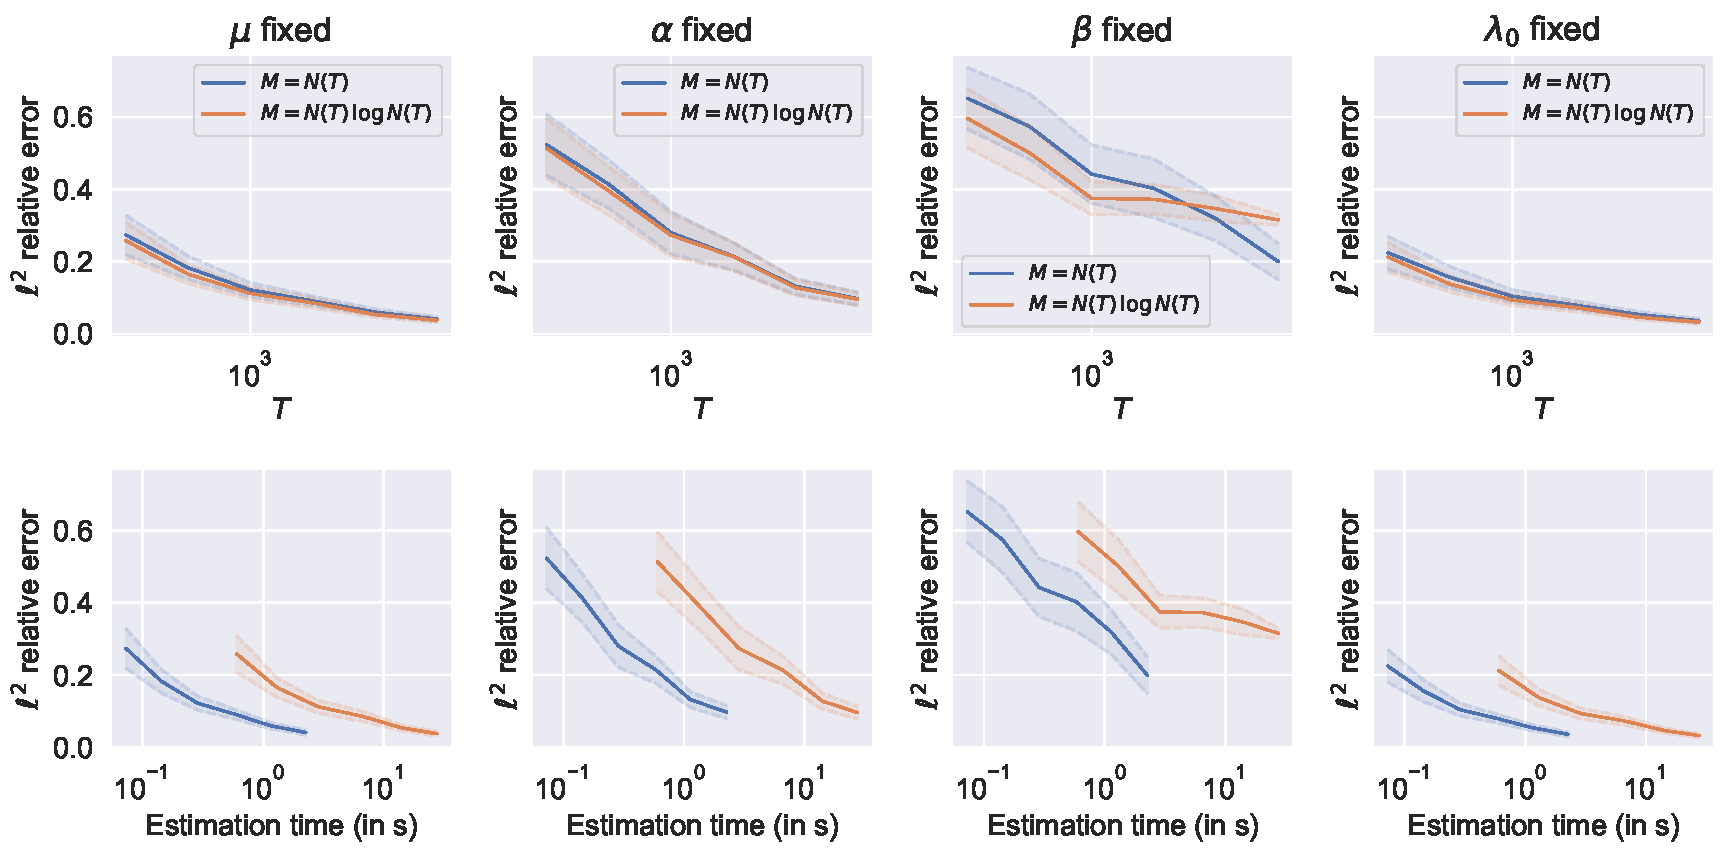
\includegraphics[width=\textwidth]{images/chapter4//l2_error_wrt_nbpoints.pdf}
        \caption{Relative estimation error with confidence bands ($\pm 1.96$ empirical standard deviation) respectively for \(\mu\), \(\alpha\), \(\beta\) and \(\lambda_0\) fixed (columns from left to right)
        with respect to the time horizon $T$ (top) and the computation time (bottom) in logarithmic scale. Level of noise $\lambda_0 = 1.6$.}
        \label{fig:chap3_errors_wrt_T}
    \end{figure}
  



    \subsubsection{Influence of the noise level}\label{sec:chap3_influence_noise}
       Figure~\ref{fig:chap3_errors_wrt_noise_N} shows the relative error with respect to the ratio $\lambda_0/m_H$, obtained when increasing the value of $\lambda_0$ while keeping the other parameters fixed, for a given horizon $T=8000$.

       \begin{figure}[!ht]
        \centering
        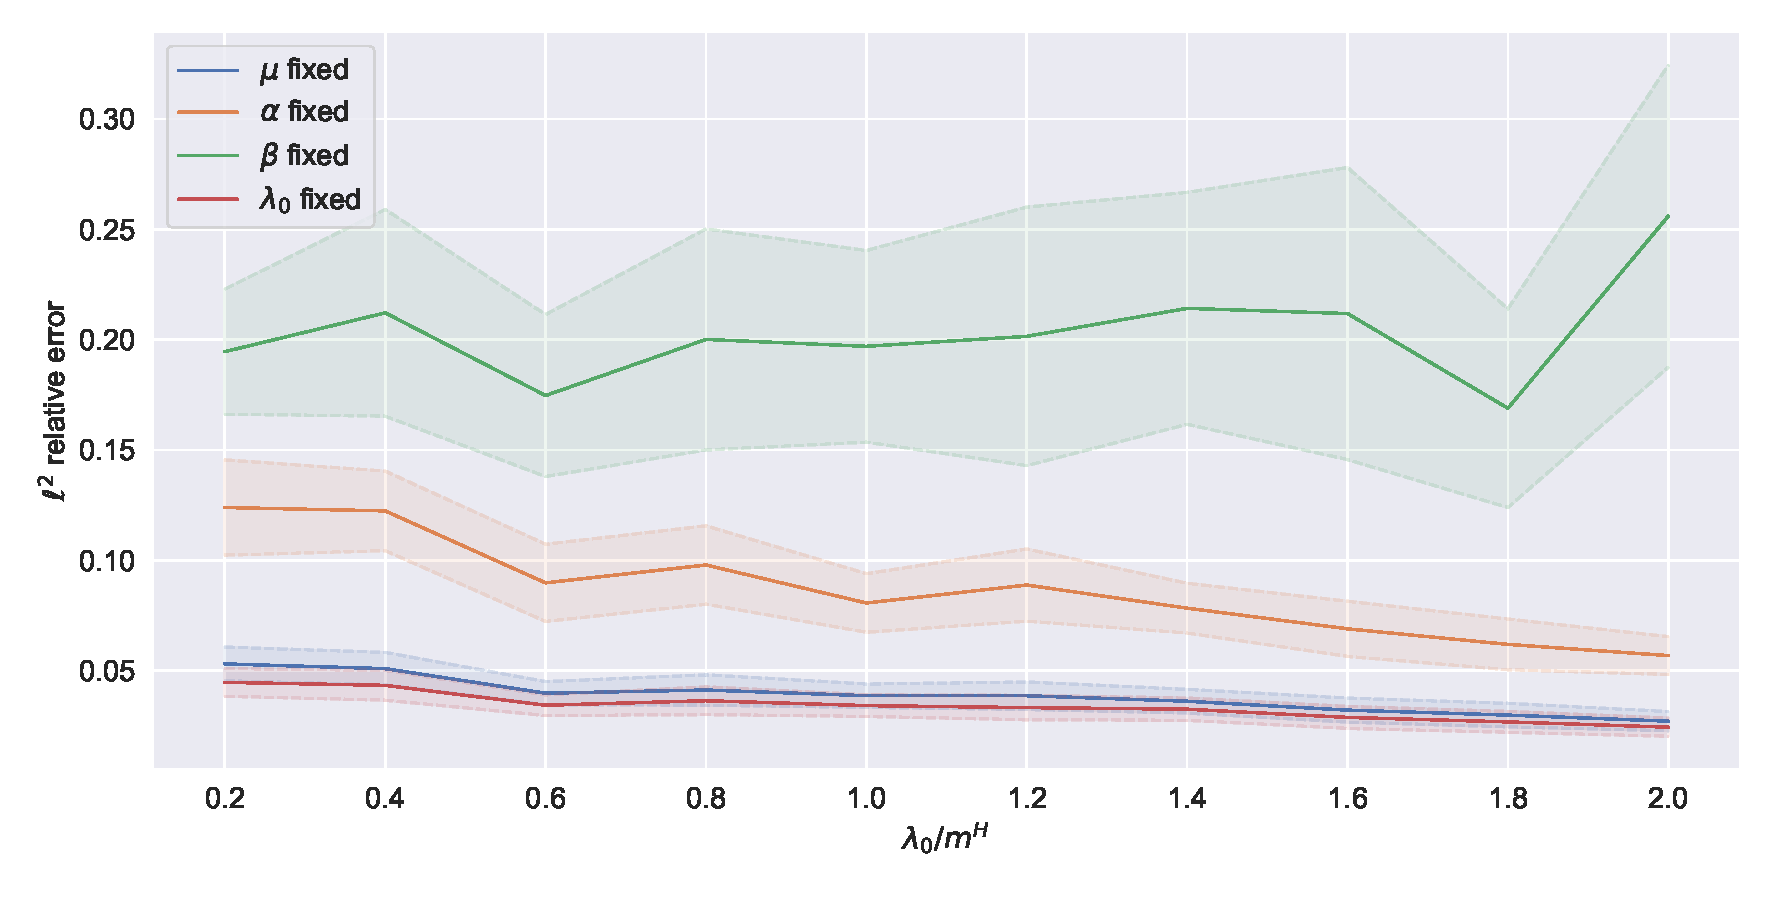
\includegraphics[width=\textwidth]{images/chapter4//vector_max_hor_wrt_noise_N.pdf}
        \caption{Relative estimation error with confidence bands ($\pm 1.96$ empirical standard deviation) respectively for \(\mu\), \(\alpha\), \(\beta\) and \(\lambda_0\) fixed 
        with respect to the noise-to-signal ratio for the maximal horizon $T=8000$.} 
        \label{fig:chap3_errors_wrt_noise_N}
        \end{figure}
        
		First, we can see that the value of $\lambda_0$ has a low impact on the quality of estimations.
   However, let us notice that when $\beta$ is fixed, the average error is substantially larger than when any of the other parameters is fixed.
     This could be explained by a compensation phenomenon inside the triplet $(\mu, \alpha,\lambda_0)$ which occurs as our method implicitly adjusts the estimation to the mean intensity of the noisy Hawkes process: 
     \[m^N = \lambda_0 + \frac{\mu}{1-\alpha},\]
     which is indeed a quantity independent of $\beta$.
    
    This numerical compensation is illustrated in Figure~\ref{fig:chap3_uni_compensation_beta_N}, where we can see that overestimating $\mu$ is systematically balanced by underestimating $\alpha$ and $\lambda_0$ and vice versa, whereas the estimated mean intensities remain accurate.
    In this experiment, the level of noise has been arbitrarily fixed to $\lambda_0 = 1.2$ but the observed behaviour appears similarly for all possible values of $\lambda_0$ used in the previous section.

    
    \begin{figure}[!ht]
        \centering
        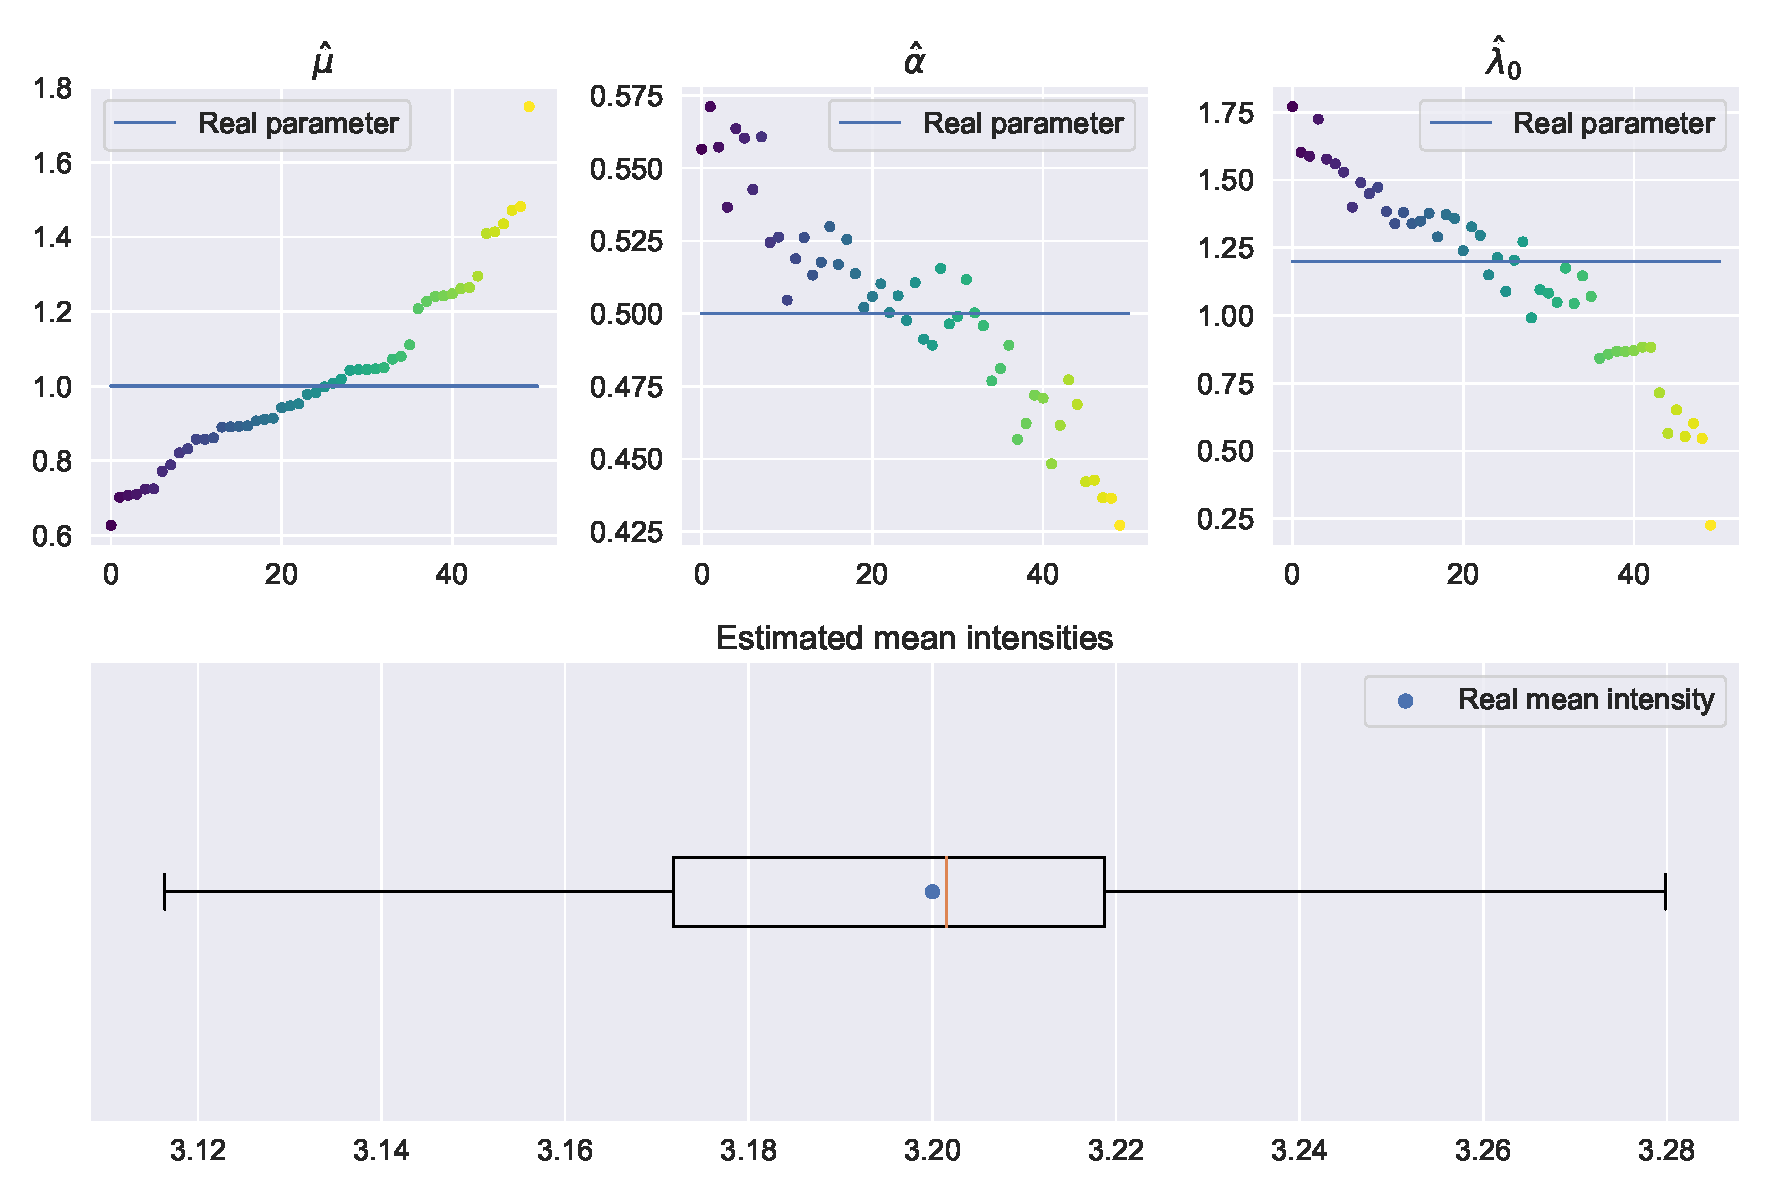
\includegraphics[width=\textwidth]{images/chapter4//compensation_beta_N.pdf}
        \caption{Estimations $\hat \mu, \hat \alpha$ and $\hat \lambda_0$ (of $\mu$, $\alpha$, and $\lambda_0$) for
        $\lambda_0 = 1.2$ when $\beta$ is fixed,
        sorted by the values of $\hat{\mu}$ (top).
        In all plots, each color corresponds to one of the 50 repetitions. Boxplot of estimated mean intensities (bottom).}
        \label{fig:chap3_uni_compensation_beta_N}
        \end{figure}

    When performing estimation with $\alpha$ fixed (the case for which the average error is the second larger, as illustrated in Figure~\ref{fig:chap3_errors_wrt_noise_N}), the compensation appears only between $\hat \mu$ and $\hat \lambda_0$ whereas $\hat \beta$ does not seem impacted, as shown in Figure~\ref{fig:chap3_uni_compensation_alpha_N}.

        \begin{figure}[!ht]
        \centering
        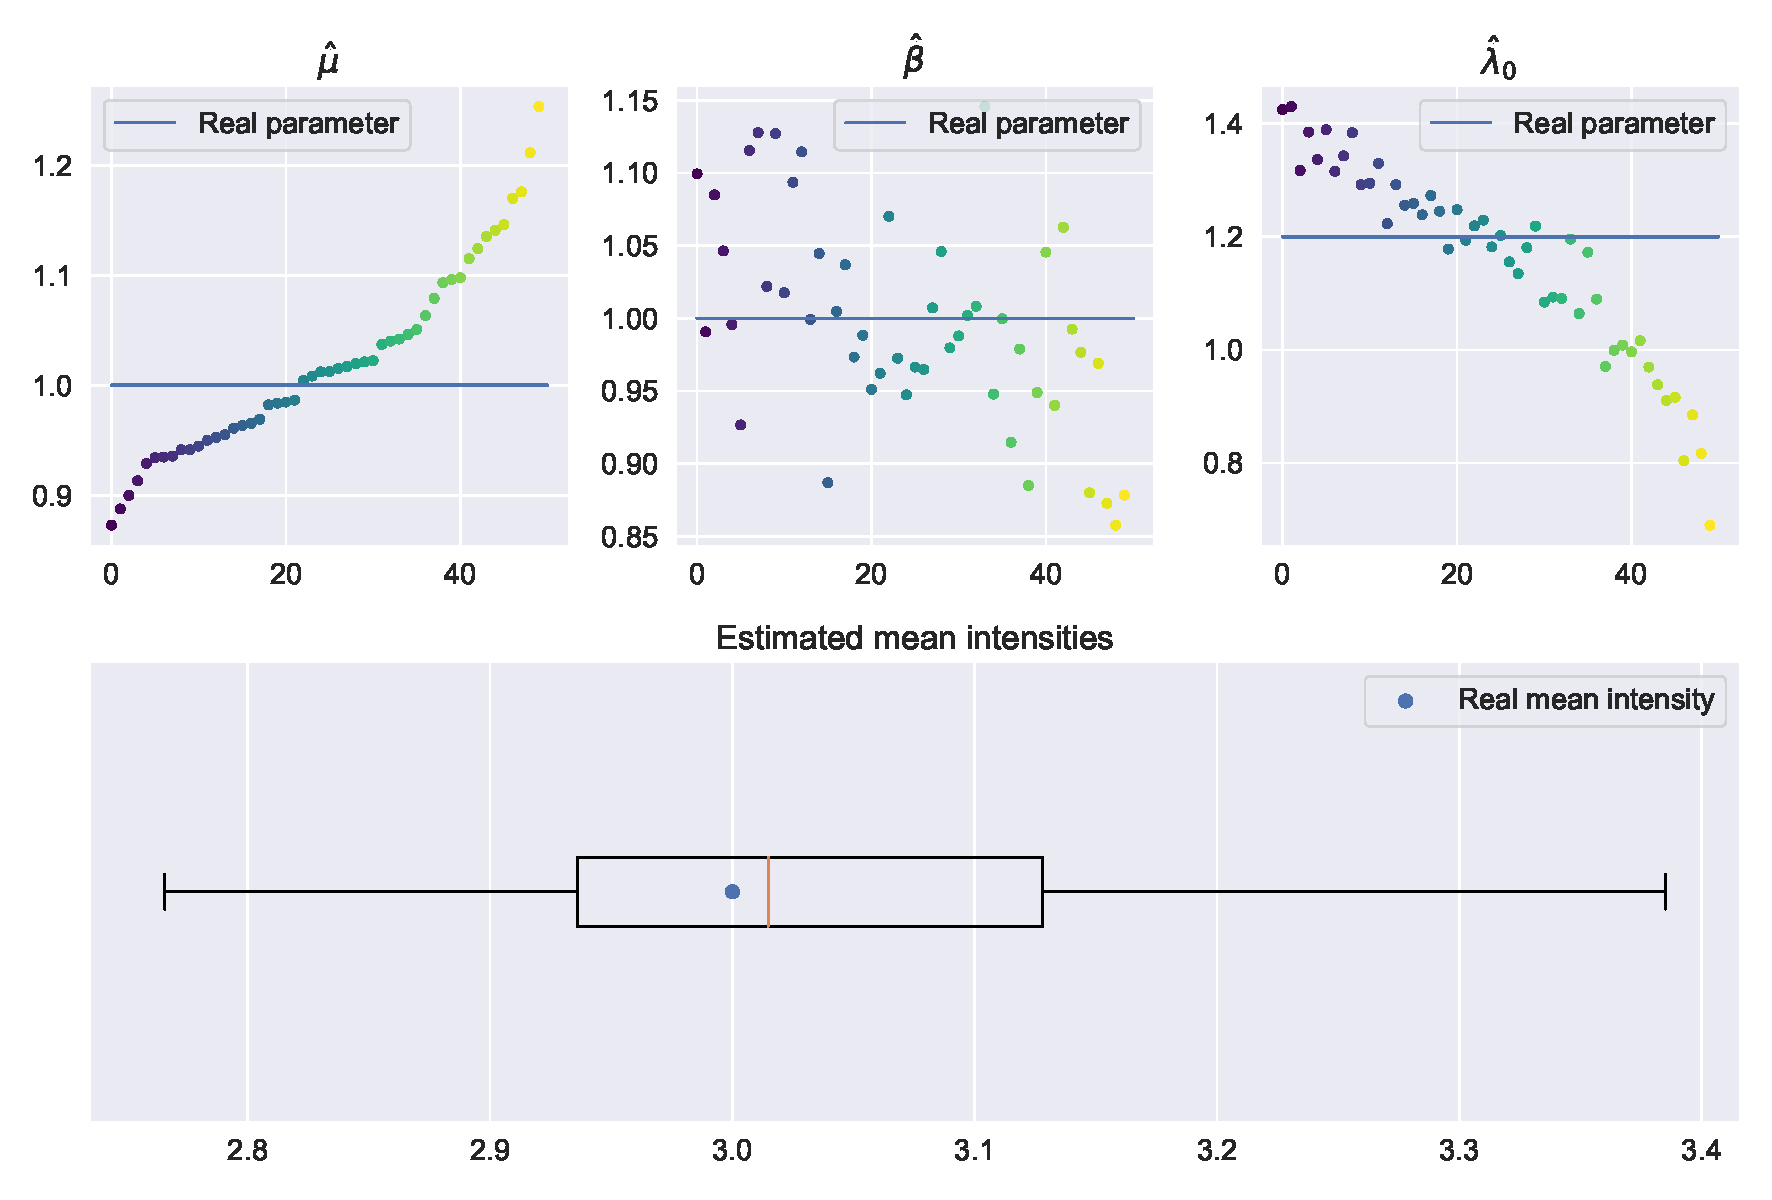
\includegraphics[width=\textwidth]{images/chapter4//compensation_alpha_N.pdf}
        \caption{Estimations $\hat \mu, \hat \beta$ and $\hat \lambda_0$ (of $\mu$, $\beta$, and $\lambda_0$) for
        $\lambda_0 = 1.2$ when $\alpha$ is fixed,
        sorted by the values of $\hat{\mu}$ (top).
        In all plots, each color corresponds to one of the 50 repetitions. Boxplot of estimated mean intensities (bottom).}
        \label{fig:chap3_uni_compensation_alpha_N}
        \end{figure}


     
        
	\subsection{Bivariate setting} \label{sec:chap3_bivariate_numerical_results}
		This section illustrates numerical estimation of bivariate exponential noisy Hawkes processes (see Section~\ref{sec:chap3_dim2}) when conditions of identifiability are met (Proposition~\ref{prop:chap3_bi_identifiable}). We carry out two different studies, exploring different scenarios: Section~\ref{sec:chap3_bi_alpha_parameter} studies the influence of the strength of the cross-interaction between the two subprocesses and Section~\ref{sec:chap3_bi_two_scenarios} investigates the performance of the estimator with and without knowledge of the null components. Indeed, since identifiability conditions depend on knowing which components are non-null, an information that is unlikely to be available in practical applications, we compare the performance of the estimator for both the reduced model $\mathcal{Q}_{\Lambda}$, where the null components are known, and the complete model, \[\mathcal Q
        = \left\{
          \mathbf{f}_{\theta}^N : \RR \to \mathbb C^{2 \times 2},
          \theta = (\mu, \alpha, \beta, \lambda_0)
          \in \RR_{>0}^2\times \RR_{\geq 0}^{2\times 2} \times \RR_{>0}^2 \times \RR_{>0}, \rho(\alpha) < 1 
       	 \right\}\,,\]with no prior information.
		
    Throughout this section, we consider a Hawkes process with $\mu = \begin{pmatrix} 1.0 \\ 1.0 \end{pmatrix}$ and $\beta = \begin{pmatrix} 1.0 \\ 1.3 \end{pmatrix}$.
    In addition, fortified by the analysis of the univariate setting,
    the Poisson intensity is chosen to be $\lambda_0 = 0.5$
    (the level of noise does not appear to have a significant impact on the quality of estimations, Figure~\ref{fig:chap3_errors_wrt_noise_N})
    and it is considered $M = N(T)$ (which provides accurate estimations in a reasonable amount of time, Figure~\ref{fig:chap3_errors_wrt_T}).
		

		\subsubsection{Influence of the cross-interaction}
		\label{sec:chap3_bi_alpha_parameter} 

        Let us consider one of the identifiable scenarios where the only non-null interaction in the Hawkes process is one of the two cross-interactions (see Proposition~\ref{prop:chap3_bi_identifiable}, Situation~\ref{hyp:chap3_bi_identifiable_1}).
        More precisely, we consider the reduced model $\mathcal{Q}_{\Lambda}$,
        where
        \[
          \Lambda = \left\{ \begin{pmatrix} 0 & 0 \\ \alpha_{21} & 0 \end{pmatrix} : \alpha_{21} > 0 \right\} \,.
        \]
        The Hawkes process is then simulated with different levels of cross-interaction: $\alpha_{21} \in \{0.2, 0.4, 0.6, 0.8\}$,
        and estimations are obtained by optimising the spectral log-likelihood on the non-null parameters $\mu_1$, $\mu_2$, $\alpha_{21}$, $\beta_2$, and $\lambda_0$.
        
        Figure~\ref{fig:chap3_bi_phase_transition} illustrates the influence of the true parameter $\alpha_{21}$ on the quality of the estimations,
	      through the relative error of the estimations for the different values of $\alpha_{21}$ and 
	      an increasing range of horizons $T$.
	      As a complement to what has been observed in Figure~\ref{fig:chap3_errors_wrt_T},
	      our estimator appears to behave particularly well for higher values of $T$, but also for higher values of $\alpha_{21}$.


        \begin{figure}[!ht]
			\centering
			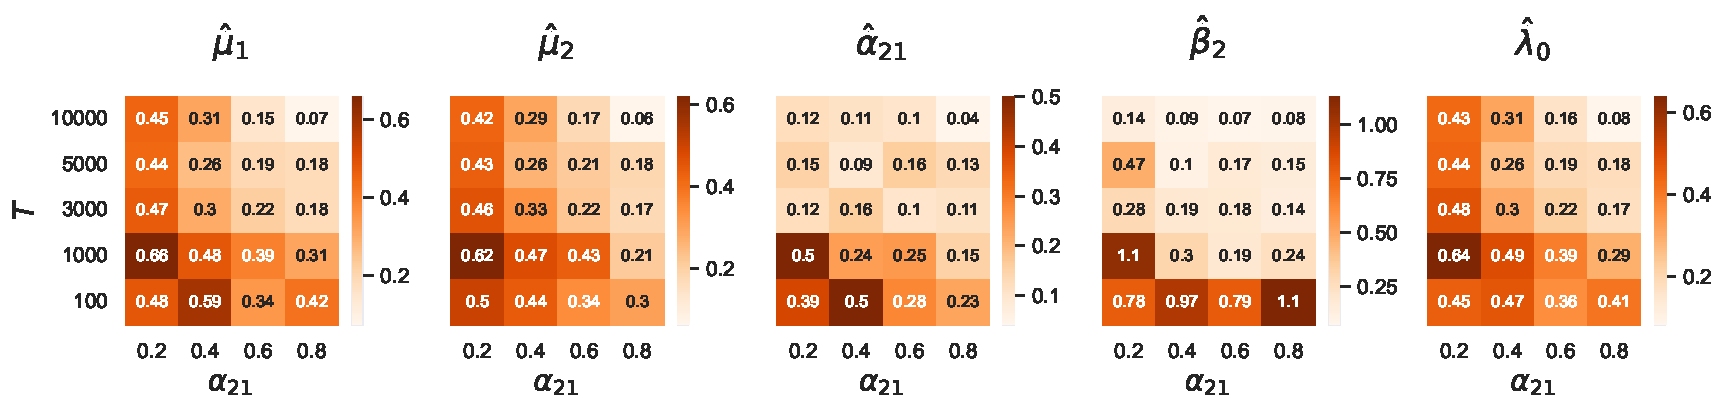
\includegraphics[width=\linewidth]{images/chapter4//phase_transition.pdf}
 		   	\caption{Heatmap of relative errors for each estimation $\hat\mu_1$, $\hat\mu_2$, $\hat\alpha_{21}$, $\hat\beta_2$, and $\hat\lambda_0$ for different levels of interaction $\alpha_{21}$ (x-axis) and horizons $T$ (y-axis).}
 		  \label{fig:chap3_bi_phase_transition}
		\end{figure}
        
        This is not surprising since, for smaller values of $\alpha_{21}$, the Hawkes process behaves closely to a homogeneous Poisson process, and as proven in Proposition~\ref{prop:chap3_bi_non_identifiable}, the superposition of two Poisson processes leads to a non-identifiable model. Lower interactions necessitate then higher values of $T$ to obtain satisfactory results. Inversely, for average and high interaction magnitudes, we start to obtain small errors for horizon values around $T=3000$. 
		
		
		\subsubsection{Influence of null interactions}
		\label{sec:chap3_bi_two_scenarios}

        In this section we simulate $50$ repetitions with a fixed horizon $T=3000$ for two identifiable scenarios regarding the Hawkes process $H = (H_1, H_2)$.
        \begin{description}
          \item[Scenario 1] The matrix of interactions is:
          \[
            \alpha = \begin{pmatrix} 0.5 & 0 \\ 0.4 & 0 \end{pmatrix}\,,
          \]
          corresponding to Proposition~\ref{prop:chap3_bi_identifiable}, Situation~\ref{hyp:chap3_bi_identifiable_1}.
          In other terms, $H_1$ excites both subprocesses whereas $H_2$ has no influence on the dynamics (See Figure~\ref{fig:chap3_bi_scenario}, left).
          \item[Scenario 2] The matrix of interactions is:
          \[
            \alpha = \begin{pmatrix} 0.5 & 0 \\ 0.4 & 0.4 \end{pmatrix}\,,
          \]
          corresponding to Proposition~\ref{prop:chap3_bi_identifiable}, Situation~\ref{hyp:chap3_bi_identifiable_2}.
          In other terms, $H_1$ excites both subprocesses and $H_2$ excites itself (See Figure~\ref{fig:chap3_bi_scenario}, right).
        \end{description}
        		
        \begin{figure}[!ht]
  			\centering
			  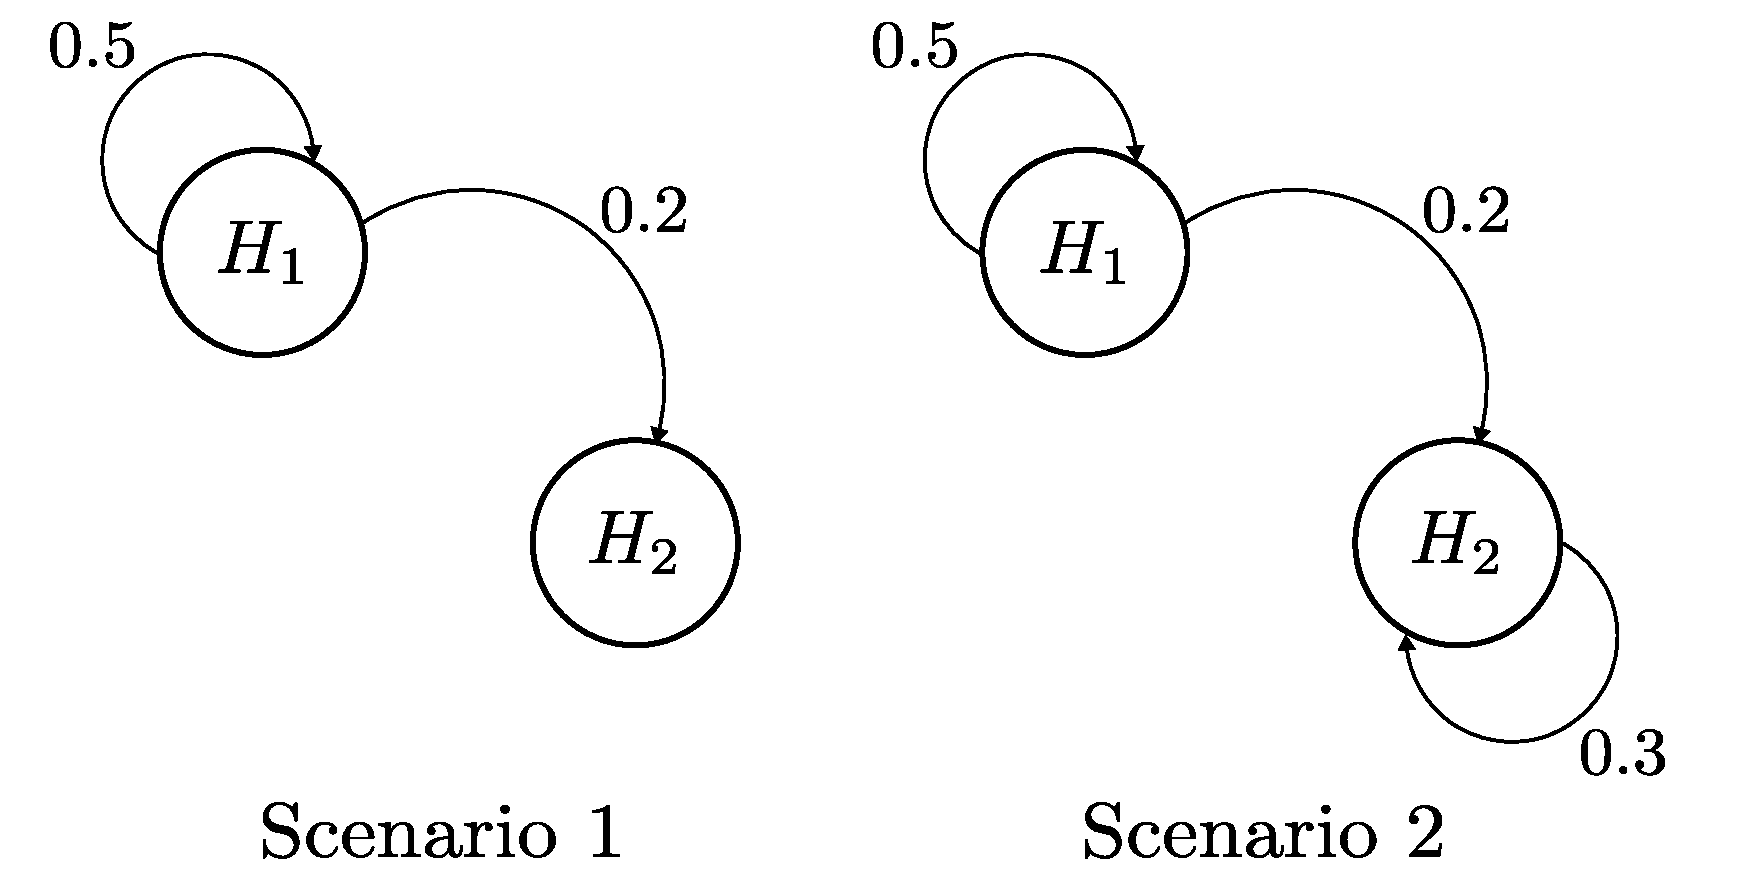
\includegraphics[width=0.5\linewidth]{images/chapter4//bivariate_spectral_hawkes.pdf}
 		   	\caption{
 		   	Interactions in the two numerical scenarios considered.
 		   	}
 		  	\label{fig:chap3_bi_scenario}
	   	\end{figure}

      Graphics in the left column of Figure~\ref{fig:chap3_column_triangle_model_estimation} present the boxplots of each parameter estimation when considering their respective reduced models $\mathcal{Q}_{\Lambda}$.		
      These results show that our method provides unbiased estimates of all parameters and is particularly efficient at inferring the interaction matrix $\alpha$ (estimations have very low variance).
      The larger variances are observed for parameters $\mu_1$, $\mu_2$ and $\lambda_0$, which is probably due to compensation effects already mentioned in Section~\ref{sec:chap3_influence_noise}.

      \begin{figure}[!ht]
        \centering
        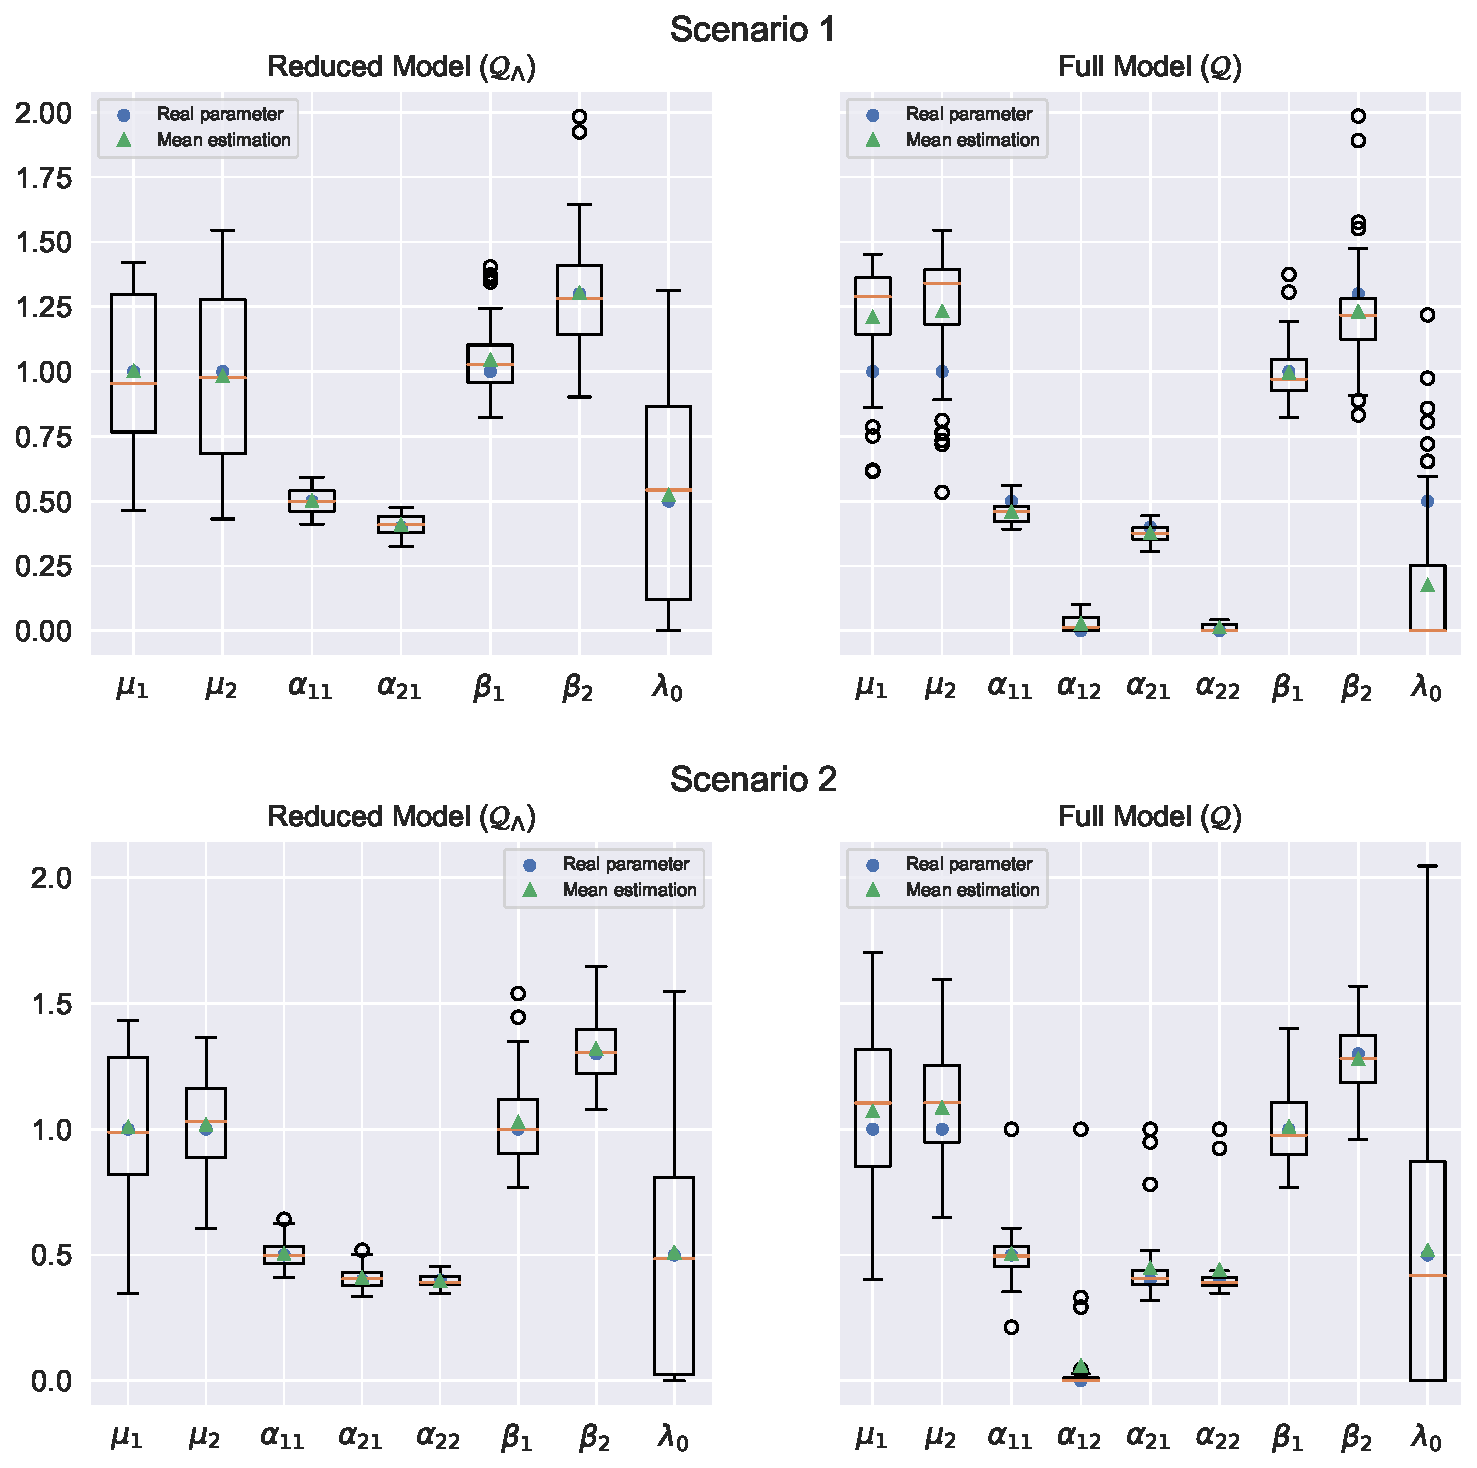
\includegraphics[width=\linewidth]{images/chapter4//column_triangle_model_estimation.pdf}
        \caption{Boxplots of parameter estimations in the reduced model $\mathcal{Q}_{\Lambda}$ (left) and full model $\mathcal{Q}$ (right)
        in Scenario~1 (top) and Scenario~2 (bottom) ($50$ trials).
        Average estimation (green triangle) is to be compared to true parameter (blue point).}
        \label{fig:chap3_column_triangle_model_estimation}
      \end{figure}
            
            Estimating in the reduced model $\mathcal Q_\Lambda$ requires prior knowledge on the null parameters $\alpha_{ij}$ ($1 \le i, j \le 2$), which is unlikely in practical applications. Therefore, we compare the results obtained in the reduced model to those in the complete model $\mathcal Q$ (see the right column graphics in Figure~\ref{fig:chap3_column_triangle_model_estimation}). If the estimates of $\alpha$ and $\beta$ seem still empirically unbiased, we observed several deteriorations compared to the previous results. First, we notice a bias in the estimates of $\mu_1$, $\mu_2$ and $\lambda_0$: more precisely, $\mu_1$ and $\mu_2$ are overestimated while $\lambda_0$ is underestimated in both scenarios. Moreover, we observe in Scenario 2 some outlier estimations for the $\alpha_{ij}$ ($1 \le i, j \le 2$) coefficients, which did not appear when considering the reduced model. 
		
		Fortunately, Figure~\ref{fig:chap3_column_triangle_model_estimation} also suggests that our estimator is able to detect the null interactions in the full model, which allows to re-estimate the parameters in the reduced model.
    To do so, we propose to look at the $5\%$-empirical quantile of each term of the estimated interaction matrix $\hat \alpha$, which are summarised in Table~\ref{tab:chap3_full_model_quantile}.

    \begin{table}[!ht]
          \centering
          \begin{tabular}{c @{\hspace{7mm}} cccc}
            \toprule
            & $\alpha_{11}$ & $\alpha_{12}$ & $\alpha_{21}$ & $\alpha_{22}$ \\
            \toprule
            Scenario 1 & 0.40 & 0.00 & 0.32 & 0.00 \\
            Scenario 2 & 0.41 & 0.00 & 0.34 & 0.35 \\
            
          \end{tabular}
          \caption{$5\%$-quantile of each parameter of the estimated interaction matrix $\hat \alpha$. The true parameter $\alpha_{12}$ is null in both scenarios and $\alpha_{22}$ is null only in Scenario 1.}
          \label{tab:chap3_full_model_quantile}
    \end{table}
    
		We can notice that the empirical $5\%$-quantiles are set to zero for each real null parameters $\alpha_{ij}$ ($1 \le i, j \le 2$) in both scenarios. 
		This suggests that when enough repetitions are available, it is possible to use these empirical quantiles to estimate the null interactions.
		An estimation procedure when no prior information is known about the support of the interaction graph would then consist in a three-step approach:
		first, estimating all parameters in the complete model $\mathcal{Q}$;
		second, computing the $5\%$-quantiles for all estimated interactions parameters in matrix $\hat \alpha$,
		and defining the support of $\alpha$ to be entries corresponding to a positive empirical quantile;
		finally, re-estimating all parameters in the reduced model defined by the support of $\alpha$.
		Let us remark that the proposed support estimation step boils down to correspond to a multiple test that,
		when the noisy Hawkes process has significantly more that $2$ dimensions,
		can be corrected thanks to usual procedures such as Bonferroni and Benjamini-Hochberg methods.
		
		\section{Discussion}

In this paper, we propose a spectral approach to estimate the parameters of a noisy Hawkes process, the performance of which is illustrated on an extended numerical study. Although we highlight the great benefit of considering a spectral analysis when standard inference methods are not available, we also bring out  identifiability issues that may arise, either from the model itself or from the spectral approach. While we exhibit several identifiable and non-identifiable scenarios in both univariate and bivariate contexts, a general result on identifiability is still to be established, in particular in higher dimensions. For this purpose, the number of non-null cross-interactions and the choice of the kernel functions appear to be key elements in order to obtain identifiability guarantees.

More generally, we believe that the spectral analysis can provide efficient estimators in many frameworks of inaccurately or partially observed data. A natural extension of this work is to consider alternative forms for the noise process, for instance an heterogeneous Poisson process. Another topic of interest is to investigate another mechanism for the noise when some points are randomly missing. This would be complementary to our work since it would allow to model both false positive and false negative occurrences. In practice, this could be of great interest for applications, especially for the tracking of epidemics. Finally, let us mention that this paper focuses on the linear Hawkes model, which excludes notably inhibition phenomenons. Though the nonlinear framework is particularly interesting for many applications, for instance in neuroscience, all the spectral theory for point processes only exists in a linear context so that we believe that developing a spectral inference procedure for nonlinear processes would be very challenging and remains a widely open topic.

\begin{subappendices}

    \section{Proof of Proposition~\ref{prop:chap3_sum_of_spectral_densities}}\label{appendix:chap3_proof_sum_spectra}
          
    \begin{lemma}\label{lemma:sum_second_order_moment}
      Let $X$ and $Y$ be two independent and stationary multivariate point processes with same dimension $d$.
      If they admit second order moment measures, denoted respectively $(M_{ij}^{X})_{1 \le i, j \le d}$ and $(M_{ij}^{Y})_{1 \le i, j \le d}$,
      then the process $N = X + Y$ also admits a second order moment measure,
      noted $(M_{ij}^N)_{1 \le i, j \le d}$,
      and for any pair $(A, B) \in (\mathcal{B}_{\RR}^c)^2$ and all $1 \le i, j \le d$:
      
      \begin{equation}\label{eq:chap3_relation_second_moment}
          M_{ij}^N(A, B) = M_{ij}^{X}(A, B) + M_{ij}^{Y}(A, B) + (m_i^X m_j^Y + m_j^X m_i^Y)\ell_\RR(A)\ell_\RR(B)\,,
      \end{equation}
      where for all $i \in \{1, \dots, d\}$ and $m_i^X = \EE[X_i([0, 1))]$ and $m_i^Y = \EE[Y_i([0, 1))]$.
      Furthermore, the reduced measure of $N$ reads:

          \begin{equation}\label{eq:chap3_relation_reduced_moment}
          \breve M_{ij}^N(B) = \breve M_{ij}^X(B) + \breve M_{ij}^Y(B)+ (m_i^X m_j^Y + m_j^X m_i^Y)\ell_{\RR}(B)\,.
      \end{equation}
     
    \end{lemma}

    \begin{proof}

    Let $(A,B)\in (\mathcal{B}_{\RR}^c)^2$. Then for any $1 \leq i,j \leq d$:
  \begin{align*}
      M_{ij}^N(A, B) &= \EE[N_i(A)N_j(B)] \\
      &= \EE[(X_i(A) + Y_i(A))(X_j(B) + Y_j(B))]\\
      &= \EE[X_i(A)X_j(B)] + \EE[X_i(A)Y_j(B)] + \EE[X_j(A)Y_i(B)] + \EE[Y_j(A)Y_j(B)]\\
      &= M_{ij}^X(A,B) + \EE[X_i(A)]\EE[Y_j(B)] + \EE[X_j(A)]\EE[Y_i(B)] + M_{ij}^Y(A,B)\\
      &= M_{ij}^X(A,B) + m_i^X m_j^Y\ell(A)\ell(B) + m_j^X m_i^Y\ell(A)\ell(B) + M_{ij}^Y(A,B)\,,
  \end{align*}
  where the last line comes from the stationarity, which implies that $\EE[X_i(A)] = m_i^X \ell(A)$.
   
      By applying Equation~\eqref{eq:chap3_reduced_moment_measure_property} to the function $g(x,y) = \II_{x \in [0,1]}\II_{y-x\in B}$ for any $B\in\mathcal{B}_\RR^c$, we can remark that:
  \begin{equation*}
      \int_{\RR^2}{g(x, y) \, M_{ij}^N(\mathrm{d}x, \mathrm{d}y)} = \int_{[0,1]}{\ell_{\RR}(\mathrm{d}x)}\int_{B}{\breve M_{ij}^N(\mathrm{d}u)} = \breve M_{ij}^N(B)\,.
  \end{equation*}
  In particular this equality is also true if we replace $N$ by $X$ and $Y$. 
      By leveraging Equation~\eqref{eq:chap3_relation_second_moment} on the left-side integral, we obtain:
  \begin{align*}
      \int_{\RR^2}{g(x, y) \, M_{ij}^N(\mathrm{d}x, \mathrm{d}y)} &= \breve M_{ij}^{X}(B) +  \breve M_{ij}^{Y}(B) + (m_i^X m_j^Y + m_j^X m_i^Y)\int_{x\in[0,1]}{\int_{y\in B + x}{\ell_\RR(\mathrm{d}y)} \, \ell_\RR(\mathrm{d}x)}  \\
      &= \breve M_{ij}^X(B) + \breve M_{ij}^Y(B)+ (m_i^X m_j^Y + m_j^X m_i^Y)\ell_{\RR}([0,1])\ell_{\RR}(B) \\
      &= \breve M_{ij}^X(B) + \breve M_{ij}^Y(B)+ (m_i^X m_j^Y + m_j^X m_i^Y)\ell_{\RR}(B) \,,
  \end{align*}
  which achieves the proof.

  \end{proof}
          
\subsubsection*{Proof of Proposition~\ref{prop:chap3_sum_of_spectral_densities}}
   By definition of the spectral density, for all $\omega\in\RR$:
   
  \begin{align}
      f_{ij}^N(\omega) = &\int_\RR \mathrm{e}^{-2\pi \iu x \omega} \, \breve M_{ij}^N(\mathrm{d}x) - m_i^N m_j^N \delta(\omega)\nonumber \\
      = &\int_\RR \mathrm{e}^{-2\pi \iu x \omega} \, \breve M_{ij}^X(\mathrm d x) + \int_\RR \mathrm{e}^{-2\pi \iu x \omega} \, \breve M_{ij}^Y(\mathrm d x)\nonumber  \\
      &+ (m_i^X m_j^Y + m_j^X m_i^Y) \int_\RR \mathrm{e}^{-2\pi \iu x \omega} \, \ell_{\RR}(\mathrm{d}x) - (m_i^X + m_i^Y)(m_j^X + m_j^Y) \delta(\omega)\nonumber  \\
      = &\int_\RR \mathrm{e}^{-2\pi \iu x \omega} \, \breve M_{ij}^X(\mathrm d x) - m_i^X m_j^X \delta(\omega) + \int_\RR \mathrm{e}^{-2\pi \iu x \omega} \, \breve M_{ij}^Y(\mathrm d x) - m_i^Y m_j^Y \delta(\omega) \nonumber \\
      &+ (m_i^X m_j^Y + m_j^X m_i^Y) \int_\RR \mathrm{e}^{-2\pi \iu x \omega} \, \ell_{\RR}(\mathrm{d}x) - (m_i^X m_j^Y + m_i^Y m_j^X) \delta(\omega) \nonumber \\
      = &f_{ij}^X(\omega) + f_{ij}^Y(\omega) + (m_i^X m_j^Y + m_j^X m_i^Y) \int_\RR \mathrm{e}^{-2\pi \iu x \omega} \,\mathrm{d}x - (m_i^X m_j^Y + m_i^Y m_j^X) \delta(\omega)\,.\label{eq:chap3_dirac_difference} 
    \end{align}
              
    By properties of the Dirac measure, for all $\omega\in\RR$:
    \[\int_\RR \mathrm{e}^{-2\pi \iu x \omega} \delta(x) \,\mathrm{d}x = 1\,,\]
    and so by duality of the Fourier transform \textcite[Proposition 5.2.4.]{Pinsky2008} it follows that:
    \[\int_\RR \mathrm{e}^{-2\pi \iu x \omega} \,\mathrm{d}x  = \delta(\omega)\,.\]

    The last two terms of Equation~\eqref{eq:chap3_dirac_difference} being equal, we obtain $f_{ij}^N = f_{ij}^X + f_{ij}^Y$.
  





\section{Proof of Proposition~\ref{prop:chap3_fixed_univariate_identifiability}}\label{appendix:chap3_identifiability_univariate}  
We first show that equality of two spectral densities with different parameters is equivalent to a system of equations (Equations~\eqref{eq:chap3_system_1d}).
This result will be used then to prove both parts of Proposition~\ref{prop:chap3_fixed_univariate_identifiability}.

Let $(\mu, \alpha, \beta, \lambda_0)$ and $(\mu', \alpha', \beta', \lambda_0')$ be two admissible $4$-tuples for the exponential noisy Hawkes model. 
      Let us assume that for all $\omega\in\RR$:
      \[
               f_{(\mu, \alpha, \beta, \lambda_0)}^N(\omega) = f_{(\mu', \alpha', \beta', \lambda_0')}^N(\omega).
      \]
      Thanks to Equation~\eqref{eq:chap3_exponential_spectral_density}, this equality implies the following system of equations:

          \begin{numcases}{}
                  \frac{\mu}{1-\alpha} + \lambda_0 = \frac{\mu'}{1-\alpha'} + \lambda_0' &\text{$(\omega\to +\infty)$}\nonumber\\
                  \frac{\mu}{1-\alpha} \frac{\beta^2 \alpha(2-\alpha)}{\beta^2(1-\alpha)^2} +\frac{\mu}{1-\alpha} + \lambda_0= \frac{\mu'}{1-\alpha'} \frac{{\beta'}^2 \alpha' (2-\alpha')}{{\beta'}^2(1-\alpha')^2} +\frac{\mu'}{1-\alpha'} + \lambda_0' &\text{$(\omega = 0)$}\nonumber\\
                  \frac{\mu}{1-\alpha} \frac{\beta^2 \alpha (2-\alpha)}{\beta^2(1-\alpha)^2 + 4\pi^2} +\frac{\mu}{1-\alpha} + \lambda_0 = \frac{\mu'}{1-\alpha'} \frac{{\beta'}^2\alpha'  (2-\alpha')}{{\beta'}^2(1-\alpha')^2 + 4\pi^2}+\frac{\mu'}{1-\alpha'} + \lambda_0' &\text{$(\omega = 1)$}.\nonumber
          \end{numcases}
          
          The first equality can be used to simplify the second and third equalities,
          leading to:
          
        \begin{numcases}{}
              \frac{\mu}{1-\alpha} + \lambda_0 = \frac{\mu'}{1-\alpha'} + \lambda_0' \nonumber\\
       \frac{\mu}{1-\alpha} \frac{\alpha (2-\alpha)}{(1-\alpha)^2} = \frac{\mu'}{1-\alpha'} \frac{\alpha' (2-\alpha')}{(1-\alpha')^2}\nonumber\\
           \frac{\mu}{1-\alpha} \frac{\beta^2 \alpha (2-\alpha)}{\beta^2(1-\alpha)^2 + 4\pi^2}= \frac{\mu'}{1-\alpha'} \frac{{\beta'}^2 \alpha' (2-\alpha')}{{\beta'}^2(1-\alpha')^2 + 4\pi^2}\,. \nonumber
        \end{numcases}
        
        Now, given that $\alpha\in(0,1)$ (same for $\alpha'$), the last two equalities lead to:
        
        \[ \frac{\beta^2(1-\alpha)^2}{\beta^2 (1-\alpha)^2 + 4\pi^2} = \frac{{\beta'}^2(1-\alpha')^2}{{\beta'}^2 (1-\alpha')^2 + 4\pi^2}\,,\]
        which in turn implies $\beta(1-\alpha) = \beta' (1-\alpha')$.
        
        Thus, it results the following system of equations:
        
         \begin{subnumcases}{\label{eq:chap3_system_1d}}
              \frac{\mu}{1-\alpha} + \lambda_0 = \frac{\mu'}{1-\alpha'} + \lambda_0' \label{eq:chap3_system_1} \\
       \frac{\mu \alpha (2-\alpha)}{(1-\alpha)^3} = \frac{\mu' \alpha' (2-\alpha')}{(1-\alpha')^3}\label{eq:chap3_system_2} \\
           \beta(1-\alpha) = \beta' (1-\alpha') \label{eq:chap3_system_3}\,.
        \end{subnumcases}
        
        Now, Equations~\eqref{eq:chap3_system_1d} lead to
        \begin{numcases}{}
        \frac{\mu}{1-\alpha} + \lambda_0 = \frac{\mu'}{1-\alpha'} + \lambda_0' \nonumber\\
          \frac{\mu}{1-\alpha} \beta^2 \alpha (2-\alpha) = \frac{\mu'}{1-\alpha'} {\beta'}^2\alpha' (2-\alpha') \nonumber\\
        \beta(1-\alpha) = \beta' (1-\alpha') \,, \nonumber
        \end{numcases}
        which, by Equation~\eqref{eq:chap3_exponential_spectral_density}, implies straightforwardly $f_{(\mu, \alpha, \beta, \lambda_0)}^N = f_{(\mu', \alpha', \beta', \lambda_0')}^N$.
        Consequently,
        \[
          f_{(\mu, \alpha, \beta, \lambda_0)}^N = f_{(\mu', \alpha', \beta', \lambda_0')}^N
          \iff
          \text{Equations~}\eqref{eq:chap3_system_1d} \,.
        \]
        
\subsubsection*{The model $\mathcal{Q}$ is not identifiable.}
            Let $\tau> -\lambda_0$ and $\lambda_0' = \lambda_0 + \tau > 0$.
    
            Then, by denoting $\kappa = \frac{\mu}{1-\alpha} \beta^2\alpha (2-\alpha)$, Equations~\eqref{eq:chap3_system_1d} are equivalent to:
            \begin{equation}\label{eq:chap3_system_non_identifiable_1d}
            \begin{cases}
              \mu' = \frac{\beta(1-\alpha) (\frac{\mu}{1-\alpha}-\tau)}{\sqrt{\beta^2(1-\alpha)^2 + \frac{\kappa}{\frac{\mu}{1-\alpha}-\tau}}} \\
              \alpha' = 1 - \frac{\beta(1 - \alpha)}{\sqrt{\beta^2(1-\alpha)^2 + \frac{\kappa}{\frac{\mu}{1-\alpha}-\tau}}} \\
              \beta' = \sqrt{\beta^2(1-\alpha)^2 + \frac{\kappa}{\frac{\mu}{1-\alpha}-\tau}}\,.
            \end{cases}
            \end{equation}
      From \eqref{eq:chap3_system_non_identifiable_1d}, it is clear that for all $\tau\in \left(-\lambda_0, \frac{\mu}{1-\alpha} \right)\setminus\{0\}$,
            $(\mu', \alpha', \beta', \lambda_0 + \tau) \neq (\mu, \alpha, \beta, \lambda_0) $ is an admissible parameter for $\mathcal Q$ and
            $f_{(\mu', \alpha', \beta', \lambda_0 + \tau)}^N = f_{(\mu, \alpha, \beta, \lambda_0)}^N$.
            Consequently, $\mathcal Q$ is not identifiable.
            
                              
\subsubsection*{The reduced model defined by a triplet of admissible parameters is identifiable.}
                  
  It will be shown that, for admissible parameters, $f_{(\mu, \alpha, \beta, \lambda_0)}^N = f_{(\mu', \alpha', \beta', \lambda_0')}^N$ implies \[\mu = \mu' \iff \alpha = \alpha' \iff \beta = \beta' \iff \lambda_0 = \lambda_0'\,,\]
  from which we can deduce identifiability of the four collections of models mentioned in Proposition~\ref{prop:chap3_fixed_univariate_identifiability}.
      Indeed, let, for instance, $\alpha^\circ \in (0, 1)$ and consider
  \[\mathcal{Q}_{\alpha} = \left\{f_{(\mu, \alpha, \beta, \lambda_0)}^N \in \mathcal{Q}, \alpha = \alpha^\circ \right\}\,.\]
  Then for all $f_{(\mu, \alpha, \beta, \lambda_0)}^N \in \mathcal Q_\alpha$ and $f_{(\mu', \alpha', \beta', \lambda_0')}^N \in \mathcal Q_\alpha$,
  \[
    f_{(\mu, \alpha, \beta, \lambda_0)}^N = f_{(\mu', \alpha', \beta', \lambda_0')}^N \implies 
  \begin{dcases}
  \mu = \mu' \iff \alpha = \alpha' \iff \beta = \beta' \iff \lambda_0 = \lambda_0'\\
  \alpha = \alpha^\circ = \alpha'
  \end{dcases} \implies
  \begin{dcases}
  \mu = \mu'\\
  \beta = \beta'\\
  \lambda_0=\lambda_0'\\
  \alpha = \alpha'\,.
  \end{dcases}
  \]
  
  So, let us assume that $f_{(\mu, \alpha, \beta, \lambda_0)} = f_{(\mu', \alpha', \beta', \lambda_0')}$,
  for some admissible parameters.
  As shown beforehand this implies Equations~\eqref{eq:chap3_system_1d}.
  From Equation~\eqref{eq:chap3_system_3}, we establish that \[\alpha = \alpha' \iff \beta = \beta'\,,\] since, $\beta > 0$ and $\alpha < 1$.
  
  From Equation~\eqref{eq:chap3_system_2}, since $\alpha > 0$, it is clear that $\alpha = \alpha' \implies \mu = \mu'$.  Conversely, if $\mu=\mu' > 0$, Equation~\eqref{eq:chap3_system_2} becomes:
  \[g(\alpha) =  \frac{\alpha (2-\alpha)}{(1-\alpha)^3} = \frac{\alpha' (2-\alpha')}{(1-\alpha')^3}  = g(\alpha')\,.\]
  In particular, $g$ is a strictly increasing function on $(0,1)$ and so it can be deduced that $\alpha = \alpha'$. So \[\mu = \mu' \iff \alpha = \alpha'\,.\]
  
  Finally, as $\mu = \mu' \iff \alpha = \alpha'$, from Equation~\eqref{eq:chap3_system_1} we conclude that $\alpha = \alpha' \implies \lambda_0 = \lambda_0'$. 
  Let us now assume that $\lambda_0 = \lambda_0'$, Equation~\eqref{eq:chap3_system_1} then reads \[\frac{\mu}{1-\alpha} = \frac{\mu'}{1-\alpha'}\,.\]
  As $\mu > 0$ and $\mu' > 0$, Equation~\eqref{eq:chap3_system_2} can be then reduced to \[s(\alpha) := \frac{\alpha(2-\alpha)}{(1-\alpha)^2} = \frac{\alpha(2-\alpha)}{(1-\alpha)^2} = s(\alpha')\,,\]
  where $s$ is a strictly increasing function on $(0,1)$ and so $\alpha = \alpha'$. With this we have proved that $\alpha = \alpha' \iff \lambda_0 = \lambda_0'$ which achieves the proof.






\section{Proof of Proposition~\ref{prop:chap3_statN_identifiability}}
\label{app:felix1}

Let $(\mathcal H_t^N)_{t \ge 0}$ (respectively $(\mathcal H_t^H)_{t \ge 0}$) be the natural filtration associated with $(\lambda^N(t))_{t\ge0}$ (respectively $(\lambda^H(t))_{t\ge0}$).
Let us now consider the conditional survival function of the first non-negative jump $\tau_1$ of $N$ given the past (before $0$):
for all $t \ge 0$,
\begin{align*}
  \mathbb P \left(\tau_1 > t \mid \mathcal H_0^N \right)
  &= \mathbb P \left(N(t) = 0 \mid \mathcal H_0^N \right)\\
  &= \mathbb P \left(P(t) = 0, H(t) = 0 \mid \mathcal H_0^N \right)\\
  &= \mathbb P \left(P(t) = 0 \mid \mathcal H_0^N \right) \mathbb P \left( H(t) = 0 \mid \mathcal H_0^N \right) & (\text{by independence})\\
  &= \mathbb P \left(P(t) = 0 \right) \mathbb P \left( H(t) = 0 \mid \mathcal H_0^H \right) & (\text{by definition})\\
  &= \mathrm e^{-\lambda_0 t} e^{- \mu \left( t - u_t \right) - u_t \lambda^H(0)} \,,
\end{align*}
  with $u_t = {(1 - \mathrm e^{-\beta t})}{\beta^{-1}}$ and
where we have used that,
given that $H(t) = 0$,
for all $u \in [0, t]$,
\[
\lambda^H (u) = \mu + \left( \lambda^H(0) - \mu \right) \mathrm e^{-\beta u}.
\]
Let us remark that the last equality can also be deduced from \textcite[Corollary~3.3]{Dassios2011} with the same notation $u_t$:
\[
\mathbb P \left( H(t) = 0 \mid \mathcal H_0^H \right) = \exp \left( - \int_0^{u_t} \frac{\mu\beta v}{1 - \beta v} \, \dd v \right) \mathrm e^{-u_t \lambda^H(0)} \,.
\]

It appears that $\mathbb P \left(\tau_1 > t \mid \mathcal H_0^N \right)$ depends on the past only through $\lambda^H(0)$.
But $\lambda^H(0) = \lambda^N(0) - \lambda_0$ and $\lambda^N(0)$ is distributed according to the stationary distribution of $\left( \lambda^N(t) \right)_{t \ge 0}$.
It results that $\lambda^H(0)$ is distributed according to the stationary distribution of $\left( \lambda^H(t) \right)_{t \ge 0}$, the Laplace transform of which is given by \textcite[Corollary 3.1]{Dassios2011}.
Plugging in this result, we have:
\begin{align*}
  \mathbb P \left(\tau_1 > t \right)
  &= \mathrm e^{-\lambda_0 t - \mu \left( t - u_t \right)} \mathbb E \left[ \mathrm e^{- u_t \lambda^H(0)} \right]\\
  &= \mathrm e^{-\lambda_0 t - \mu \left( t - u_t \right)} \exp \left( - \int_0^{u_t} \frac{\mu\beta v}{\beta v + \mathrm e^{-\alpha\beta v} - 1} \dd v \right) \,.
\end{align*}	
For ease of derivation, let $G : t \in \RR_{\ge 0} \mapsto - \log \mathbb P \left(\tau_1 > t \right)$.
The function $G$ is differentiable and has derivative $D$ given by:
\[
D(t) = \lambda_0 + \mu \left( 1 - \mathrm e^{-\beta t} \right) + \frac{\mu \left( 1 - \mathrm e^{-\beta t} \right) \mathrm e^{-\beta t}}{\exp \left(-\alpha \left( 1 - \mathrm e^{-\beta t} \right) \right) - \mathrm e^{-\beta t}} \,.
\]

Now define in the same manner $\tau_1'$, $G'$, and $D'$ from the process $N'$ with parameter $(\mu', \alpha', \beta', \lambda_0')$, with $\lambda^{N'}(0)$ being distributed according to the stationary distribution of $\bigl( \lambda^{N'}(t) \bigr)_{t \ge 0}$,
and assume that $N$ and $N'$ have the same distribution.
Then it follows that both $\tau_1$ and $\tau_1'$ have the same distribution, so that $G(t) = G'(t)$ for all $t \ge 0$.
Since $G$ and $G'$ are everywhere differentiable and have the same initial value $G(0) = G'(0) = 0$, it results that $D(t) = D'(t)$ for all $t \ge 0$.

We want to establish a system of four equations satisfied by the parameters that leads to the equality of the 4-tuples.
First, noting that $\lim_{t \to \infty} D(t) = \lambda_0 + \mu$, we get 
\begin{equation}\label{eq:chap3_statN_eq_1}
\lambda_0 + \mu = \lambda_0' + \mu' \,.
\end{equation}
Then, since $\lim_{t \to 0} D(t) = \lambda_0 + \mu / (1 - \alpha)$, we get, using Equation~\eqref{eq:chap3_statN_eq_1},
\begin{equation}\label{eq:chap3_statN_eq_2}
\frac{\mu\alpha}{1 - \alpha} = \frac{\mu'\alpha'}{1 - \alpha'} \,.
\end{equation}

To highlight two other equations on the parameters, we establish the Taylor expansion of $D(t)$ around $t = 0$ up to order 2.
After some calculation, we find that 
\begin{equation*}
  D(t) = \lambda_0 + \frac{\mu}{1-\alpha} + \frac{\mu\alpha}{1-\alpha} \left( \frac{1}{2} \beta t \frac{\alpha-2}{1-\alpha} + \frac{1}{12} \beta^2 t^2 \frac{\alpha^3 - \alpha^2 - 3\alpha + 6}{(1-\alpha)^2} + o\bigl(t^2\bigr) \right) \,.
\end{equation*}
From the first-order term of the expansion, Equation~\eqref{eq:chap3_statN_eq_2} and the equality of $D$ and $D'$, we find that
\begin{equation}\label{eq:chap3_statN_eq_3}
  \beta \frac{\alpha - 2}{1 - \alpha} = \beta' \frac{\alpha' - 2}{1 - \alpha'} \,.
\end{equation}
Then the second-order term of the expansion can be rewritten
\begin{equation*}
  \frac{\mu\alpha}{1-\alpha} \frac{1}{12} \left( \frac{\beta(\alpha-2)}{1-\alpha} \right)^2 \frac{\alpha^3 - \alpha^2 - 3\alpha + 6}{(\alpha-2)^2} \,,
\end{equation*}
so that from Equations~\eqref{eq:chap3_statN_eq_2} and \eqref{eq:chap3_statN_eq_3}, we find that 
\begin{equation}\label{eq:chap3_statN_eq_4}
  g(\alpha) = \frac{\alpha^3 - \alpha^2 - 3\alpha + 6}{(\alpha-2)^2} = \frac{\alpha'^3 - \alpha'^2 - 3\alpha' + 6}{(\alpha'-2)^2} = g(\alpha') \,.
\end{equation}
$\alpha \mapsto g(\alpha)$ can be shown to be strictly increasing for $\alpha \in (0, 1)$, so that Equation~\eqref{eq:chap3_statN_eq_4} yields that $\alpha = \alpha'$.
With this remark, one can easily show from the system composed by Equations~\eqref{eq:chap3_statN_eq_1}--\eqref{eq:chap3_statN_eq_4} that the tuples $(\mu, \alpha, \beta, \lambda_0)$ and $(\mu', \alpha', \beta', \lambda_0')$ are equal.


\section{Proof of Proposition~\ref{prop:chap3_rectangle}}
\label{app:felix3}

\begin{lemma}\label{lemma:taylor}
Assume all moments of $h$ are finite: $\forall n \ge 0, m_n = \int t^n h(t) \, \dd t < \infty$.
Then
the spectral density $f^N$ of the noisy Hawkes process $N$ has a Taylor expansion around $0$ given by:
\begin{equation}\label{eq:chap3_taylor}
\forall t \in \RR: \quad
  f^N(t) = \frac{\mu}{(1-\alpha)^3} + \frac{\mu}{(1-\alpha)^3} \sum_{q \ge 1} \left( \frac{\alpha}{1 - \alpha} \sum_{n \ge 1} b_n t^{2n} \right)^q + \lambda_0 \,,
\end{equation}
with 
\begin{equation}\label{eq:chap3_taylor_an_bn}
  b_n = \frac{(-1)^n (2\pi)^{2n} a_n}{(2n)!} \,, \qquad \text{and} \qquad
  a_n = 2 m_{2n} - \frac{\alpha}{1 - \alpha} \sum_{k=1}^{2n-1} \binom{2n}{k} (-1)^k m_k m_{2n-k} \,.
\end{equation}
\end{lemma}
\begin{proof}
Introduce the Taylor expansion of the Fourier transform of $h$:
\begin{equation*}
\forall t \in \RR: \quad
  \tilde h(t) = \sum_{n \ge 0} (\iu \tau)^n \frac{m_n}{n!},
\end{equation*}
where $\tau = -2 \pi t$.
Then, given that $m_0=1$,
\begin{align*}
  \left \lvert 1 - \alpha \tilde h(t) \right \rvert^2 
  &= \left( 1 - \alpha \sum_{n \ge 0} (\iu \tau)^n \frac{m_n}{n!} \right) \left( 1 - \alpha \sum_{n \ge 0} (-\iu \tau)^n \frac{m_n}{n!} \right)\\
  &= 1 - 2 \alpha \sum_{n \ge 0} (-1)^n \tau^{2n} \frac{m_{2n}}{(2n)!} + \alpha^2 \sum_{n \ge 0} \sum_{k=0}^n (-1)^k (\iu \tau)^n \frac{m_{n-k}m_k}{(n-k)!k!}\\
  &= 1 - \alpha \sum_{n \ge 0} 2 m_{2n} \frac{(-1)^n \tau^{2n}}{(2n)!} + \alpha^2 \sum_{n \ge 0} \sum_{k=0}^{2n} (-1)^k m_k m_{2n-k} \binom{2n}{k} \frac{(-1)^n \tau^{2n}}{(2n)!}\\
  &= (1 - \alpha)^2 \left( 1 - \frac{\alpha}{1 - \alpha} \sum_{n \ge 1} a_n \frac{(-1)^n \tau^{2n}}{(2n)!} \right).
\end{align*}

Inverting this expression and taking the Taylor expansion of $x \mapsto (1 - x)^{-1}$ around 0 yields the desired result.
\end{proof}

\begin{remark}
For $n = 1, 2$, $a_n$ is given by
\[
\begin{cases}
    a_1 &= 2 m_2 + \frac{\alpha}{1 - \alpha} 2 m_1^2 \\
    a_2 &= 2 m_4 + \frac{\alpha}{1 - \alpha} \bigl(8 m_1 m_3 - 6 m_2^2\bigr) \,,
\end{cases}
\]
so that the Taylor expansion of $f^N$ up to order $5$ is:
\begin{equation*}
  f^N(t) = a + c_1 t^2 + c_2 t^4 + o(t^5) \,,
\end{equation*}
with
\begin{align*}
a &= \frac{\mu}{(1-\alpha)^3} + \lambda_0 \\
  c_1 &= 4 \frac{\mu\alpha \pi^2}{(1-\alpha)^4} \left[ - m_2 - \frac{\alpha}{1 - \alpha} m_1^2 \right]\\
  c_2 &= 16 \frac{\mu\alpha \pi^4}{(1-\alpha)^4} \left[ \frac{m_4}{12} + \frac{\alpha}{1 - \alpha} \left( \frac{m_1 m_3}{3} + \frac{3 m_2^2}{4} \right) + \left( \frac{\alpha}{1 - \alpha} \right)^2 2 m_2 m_1^2 + \left( \frac{\alpha}{1 - \alpha} \right)^3 m_1^4 \right] \,.
\end{align*}
\end{remark}

\subsubsection*{Proof of Proposition~\ref{prop:chap3_rectangle}}
Let $(\mu, \alpha, \phi, \lambda_0)$ and $(\mu', \alpha', \phi', \lambda_0')$ be two admissible $4$-tuples for the uniform noisy Hawkes model $\mathcal R$, and assume that, for all $\omega \in \mathbb R$,
\begin{equation*}
  f_{(\mu, \alpha, \phi, \lambda_0)}^N(\omega) = f_{(\mu', \alpha', \phi', \lambda_0')}^N(\omega)\,.
\end{equation*}
First, noting that $\lim_{\omega\to\infty} f_{(\mu, \alpha, \phi, \lambda_0)}^N(\omega) = \lambda_0 + \mu/(1 - \alpha)$, we get
\begin{equation}\label{eq:chap3_idunif_eq1}
  \lambda_0 + \frac{\mu}{1 - \alpha} = \lambda_0' + \frac{\mu'}{1 - \alpha'}\,.
\end{equation}
Then, since $f_{(\mu, \alpha, \phi, \lambda_0)}^N(0) = \lambda_0 + \mu/(1-\alpha)^3$ and using Equation~\eqref{eq:chap3_idunif_eq1}, we get:
\begin{equation}\label{eq:chap3_idunif_eq2}
  \frac{\mu\alpha(2-\alpha)}{(1-\alpha)^3} = \frac{\mu'\alpha'(2-\alpha')}{(1-\alpha')^3}\,.
\end{equation}

Now, since the Taylor expansions, given by Equation~\eqref{eq:chap3_taylor}, of $f_{(\mu, \alpha, \phi, \lambda_0)}^N$ and $f_{(\mu', \alpha', \phi', \lambda_0')}^N$ around 0 coincide, their respective Taylor coefficients $(c_1, c_2, \ldots)$ and $(c_1', c_2', \ldots)$ are equal.
Plugging in the moments of the uniform distribution on $[0, \phi]$, 
\begin{equation*}
  m_n = \frac{\phi^n}{n+1}\,, \qquad \text{for all}~n \ge 0\,,
\end{equation*}
the first order coefficient $c_1$ can be written
\begin{equation*}
  c_1 = - \frac{\pi}{3} \frac{\mu\alpha(2-\alpha)}{(1-\alpha)^3} \phi^2 \frac{4-\alpha}{(1-\alpha)^2 (2-\alpha)}\,,
\end{equation*}
so that, with the use of Equation~\eqref{eq:chap3_idunif_eq2}, we get
\begin{equation}\label{eq:chap3_idunif_eq3}
  \phi^2 \frac{4-\alpha}{(1-\alpha)^2 (2-\alpha)} = \phi'^2 \frac{4-\alpha'}{(1-\alpha')^2 (2-\alpha')}\,.
\end{equation}
Similarly, by plugging the moments in the second order coefficient $c_2$, we get 
\begin{equation*}
  c_2 = \frac{\pi^4}{15} \frac{\mu\alpha(2-\alpha)}{(1-\alpha)^3} \left( \phi^2 \frac{4-\alpha}{(1-\alpha)^2(2-\alpha)} \right)^2 \frac{(2-\alpha)(\alpha^3 - 8\alpha^2 + 18\alpha + 4)}{(4 - \alpha)^2}\,,
\end{equation*}
so that, by Equations \eqref{eq:chap3_idunif_eq2} and \eqref{eq:chap3_idunif_eq3},
\begin{equation}\label{eq:chap3_idunif_eq4}
  g(\alpha) = \frac{(2-\alpha)(\alpha^3 - 8\alpha^2 + 18\alpha + 4)}{(4 - \alpha)^2} = \frac{(2-\alpha')(\alpha'^3 - 8\alpha'^2 + 18\alpha' + 4)}{(4 - \alpha')^2} = g(\alpha')\,.
\end{equation}
But $\alpha \mapsto g(\alpha)$ can be shown to be strictly increasing for $\alpha \in (0, 1)$, so that Equation~\eqref{eq:chap3_idunif_eq4} yields that $\alpha = \alpha'$.
Finally, it is easily proven from the system composed by Equations~\eqref{eq:chap3_idunif_eq1}--\eqref{eq:chap3_idunif_eq4} that the tuples $(\mu, \alpha, \beta, \lambda_0)$ and $(\mu', \alpha', \beta', \lambda_0')$ are equal.


\section{Proof of Proposition~\ref{prop:chap3_bi_non_identifiable}}\label{appendix:chap3_bi_non_identifiable}

Let $N$ be a bivariate noisy Hawkes process parametrised by the exponential model $\mathcal{Q}_\Lambda$. We will prove that if either of the conditions in Proposition~\ref{prop:chap3_bi_non_identifiable} is fulfilled then $\mathcal{Q}_\Lambda$ is not identifiable.

\begin{itemize}

\item \textbf{Condition~\ref{hyp:chap3_bi_non_identifiable_1}:} Let 
\[\Lambda = \left\{ \begin{pmatrix} \alpha_{11} & 0 \\ 0 & \alpha_{22} \end{pmatrix}, 0 \le \alpha_{11}, \alpha_{22} < 1 \right\}\,.\]
For any admissible $\theta = (\mu, \alpha, \beta, \lambda_0)$, the spectral matrix $\mathbf{f}_{\theta}^N$ is diagonal such that, for any integer $i\in\{1,2\}$:

\[{ f_{\theta}^N }_{ii}(\omega) = \frac{\mu_i}{1-\alpha_{ii}}\left(\frac{\beta_i^2 \alpha_{ii} (2-\alpha_{ii})}{\beta_i^2 (1-\alpha_{ii})^2 + 4 \pi^2 \omega^2} \right) + \left(\frac{\mu_i}{1-\alpha_{ii}} + \lambda_0\right)\,.\] 

We will show that there exists an admissible $\theta' = (\mu', \alpha', \beta', \lambda_0')$ such that $\theta'\neq \theta$ and $\mathbf{f}_\theta^N = \mathbf{f}_{\theta'}^N$. Let $\tau > -\lambda_0$ and $\lambda_0' = \lambda_0 + \tau$.

For every $i\in\{1,2\}$,
on the one hand, if $\alpha_{ii}\neq 0$ then, as shown in the univariate case (Appendix~\ref{appendix:chap3_identifiability_univariate}),
letting $\kappa_i = \frac{\mu_i}{1-\alpha_{ii}}\beta_i^2 \alpha_{ii} (2-\alpha_{ii})$ and defining the parameters:
\begin{equation}
\begin{cases}
\mu_i' = \frac{\beta_i(1-\alpha_{ii}) (\frac{\mu_i}{1-\alpha_{ii}}-\tau)}{\sqrt{\beta_i^2(1-\alpha_{ii})^2 + \frac{\kappa_i}{\frac{\mu_i}{1-\alpha_{ii}}-\tau}}} \\
\alpha_{ii}' = 1 - \frac{\beta_i(1 - \alpha_{ii})}{\sqrt{\beta_i^2(1-\alpha_{ii})^2 + \frac{\kappa_i}{\frac{\mu_i}{1-\alpha_{ii}}-\tau}}} \\
\beta_i' = \sqrt{\beta_i^2(1-\alpha_{ii})^2 + \frac{\kappa_i}{\frac{\mu_i}{1-\alpha_{ii}}-\tau}}\,,
\end{cases}
\end{equation}
leads to ${ f_{\theta}^N }_{ii} = { f_{\theta'}^N }_{ii}$.

On the other hand, if $\alpha_{ii}=0$ then,
${ f_{\theta}^N }_{ii} = \mu_i + \lambda_0$ and it is enough to consider:
\[
\begin{cases}
\mu_i' = \mu_i - \tau \\
\alpha_{ii}' = 0 \\
\beta_i' = \beta_i\,,
\end{cases}
\]
to get ${ f_{\theta}^N }_{ii} = { f_{\theta'}^N }_{ii}$.

In both cases, for $\tau \in\left(-\lambda_0, \min_{1\leq i \leq 2}\left\{\frac{\mu_i}{1-\alpha_{ii}}\right\} \right)\setminus\{0\}$, we obtain an admissible parameter $\theta' \neq \theta$ and
$\mathbf{f}_\theta^N = \mathbf{f}_{\theta'}^N$.
Thus, the model is not identifiable.






\item \textbf{Condition~\ref{hyp:chap3_bi_non_identifiable_2} and \ref{hyp:chap3_bi_non_identifiable_2_bis}:} 
Without loss of generality, let 
\[\Lambda = \left\{ \begin{pmatrix} \alpha_{11} & \alpha_{12} \\ 0 & 0 \end{pmatrix}, 0 < \alpha_{11} < 1, \alpha_{12} > 0 \right\}\,.\] 

For any admissible parameter $\theta = (\mu, \alpha, \beta, \lambda_0)$ and for any $\omega\in\RR$, the spectral matrix reads: 

\begin{equation*}
\mathbf{f}_\theta^N(\omega) = 
\begin{bmatrix}
  {f_\theta^N}_{11}(\omega) & {f_\theta^N}_{12}(\omega)\\
  {f_\theta^N}_{21}(\omega) & {f_\theta^N}_{22}(\omega)
\end{bmatrix}	=
\begin{bmatrix}
  {f_\theta^N}_{11}(\omega) &  \dfrac{\mu_2 \beta_1 \alpha_{12}}{\beta_1(1-\alpha_{11}) - 2 \pi \iu \omega}\\
   \dfrac{\mu_2 \beta_1 \alpha_{12}}{\beta_1(1-\alpha_{11}) + 2 \pi \iu \omega} & \mu_2 + \lambda_0
\end{bmatrix}
\end{equation*}
with 
\begin{align*}
{f_\theta^N}_{11}(\omega) = &\left(\dfrac{\mu_1}{1-\alpha_{11}} + \dfrac{\mu_2\alpha_{12}}{1-\alpha_{11}} \right)\dfrac{\beta_1^2 \alpha_{11}(2-\alpha_{11})}{\beta_1^2 (1-\alpha_{11})^2 + 4 \pi^2\omega^2} + \dfrac{\mu_2 \beta_1^2 \alpha_{12}^2}{\beta_1^2 (1-\alpha_{11})^2 + 4 \pi^2\omega^2} \\
&+ \dfrac{\mu_1}{1-\alpha_{11}} + \dfrac{\mu_2\alpha_{12}}{1-\alpha_{11}} + \lambda_0\,.
\end{align*}

Let us introduce the following constants:

\begin{equation*}
\begin{cases}
  A = \mu_2 + \lambda_0\\
  B = \mu_2 \beta_1 \alpha_{12}\\
  C = \beta_1 (1-\alpha_{11})\\
  D = \frac{\mu_1 + \mu_2 \alpha_{12}}{1-\alpha_{11}} + \lambda_0\\
  E = (\frac{\mu_1 + \mu_2 \alpha_{12}}{1-\alpha_{11}} ) \beta_1^2 \alpha_{11} (2-\alpha_{11}) + \mu_2 \beta_1^2 \alpha_{12}^2\,,
\end{cases}
\end{equation*}
which allow us to rewrite the spectral matrix as:

\begin{equation}\label{eq:chap3_bi_matrix_constants}
\mathbf{f}_\theta^N(\omega) = 
\begin{bmatrix}
  \dfrac{E}{C^2 + 4 \pi^2 \omega^2} + D & \dfrac{B}{C - 2 \pi \iu \omega}\\
  \dfrac{B}{C + 2 \pi \iu \omega} & A
\end{bmatrix}\,.
\end{equation}

Let $\tau\in\RR\setminus \left\{\mu_2, (\mu_1 + \mu_2 \alpha_{12})/(1-\alpha_{11}) \right\}$ and: \[\kappa_\tau = \frac{(\mu_1 + \mu_2 \alpha_{12})\alpha_{11}(2-\alpha_{11})(\mu_2 - \tau) - \tau\mu_2^2 \alpha_{12}^2(1-\alpha_{11})}{(\mu_2 - \tau)(\mu_1 + \mu_2\alpha_{12} - \tau(1-\alpha_{11}))}\,.\]

Now, consider the parameter $\theta' = (\mu', \alpha', \beta', \lambda_0')$, defined as follows:

\begin{equation}\label{eq:chap3_bi_system_constants}
\begin{cases}
  \mu_1' = \frac{\mu_1 - \tau(1-\alpha_{11})}{\sqrt{(1-\alpha_{11})^2 + \kappa_\tau}}\\
  \mu_2' = \mu_2 - \tau\\
  \alpha_{11}' = 1 - \frac{1-\alpha_{11}}{\sqrt{(1-\alpha_{11})^2 + \kappa_\tau}}\\
  \alpha_{12}' = \frac{\mu_2 \alpha_{12}}{(\mu_2 - \tau)\sqrt{(1-\alpha_{11})^2 + \kappa_\tau}}\\
  \beta_1' = \beta_1 \sqrt{(1-\alpha_{11})^2 + \kappa_\tau}\\
  \lambda_0' = \lambda_0 + \tau\,.
\end{cases}
\end{equation}

The goal will be to show that there exists $\tau$ such that $\theta'$ is well defined, admissible for $\mathcal Q_\Lambda$, such that $\theta\neq\theta'$ and $\mathbf{f}_\theta^N = \mathbf{f}_{\theta'}^N$.

First, in order for $\theta'$ to be an admissible parameter, let us remark that $\rho(S) = \alpha_{11}$ and so we obtain the following constrains:

\begin{equation}\label{eq:chap3_system_tau_non_identifiability}
\begin{cases}
  \mu_1' > 0\\
  \mu_2' > 0\\
  0 < \alpha_{11}' < 1\\
  \alpha_{12}' > 0\\
  \beta_1' > 0\\
  \lambda_0' >0
\end{cases}\iff
\begin{cases}
  \mu_1 - \tau(1-\alpha_{11}) > 0\\
  \mu_2 - \tau > 0\\
  \frac{1-\alpha_{11}}{\sqrt{(1-\alpha_{11})^2 + \kappa_\tau}} < 1\\
  (1-\alpha_{11})^2 + \kappa_\tau > 0\\
  \lambda_0 + \tau > 0
\end{cases}\iff
\begin{cases}
  \tau < \frac{\mu_1}{1-\alpha_{11}}\\
  \tau < \mu_2\\
  \kappa_\tau > 0\\
  \tau > -\lambda_0\,.
\end{cases}
\end{equation}

Since $\tau < \mu_1/(1-\alpha_{11}) \implies \mu_1 + \mu_2 \alpha_{12} - \tau(1-\alpha_{11}) > 0$, the third inequality becomes

\[
\tau < \frac{(\mu_1 + \mu_2 \alpha_{12})\alpha_{11}(2-\alpha_{11})\mu_2}{(\mu_1 + \mu_2 \alpha_{12})\alpha_{11}(2-\alpha_{11}) + \mu_2^2(1-\alpha_{11}) \alpha_{12}^2}\,.
\]
Then for 
\[\tau \in \left(-\lambda_0, \min\left\{\frac{\mu_1}{1-\alpha_{11}}, \mu_2,  \frac{(\mu_1 + \mu_2 \alpha_{12})\alpha_{11}(2-\alpha_{11})\mu_2}{(\mu_1 + \mu_2 \alpha_{12})\alpha_{11}(2-\alpha_{11}) + \mu_2^2(1-\alpha_{11}) \alpha_{12}^2} \right\} \right)\setminus\{0\}\,,\]
the right-hand side of Equations~\eqref{eq:chap3_system_tau_non_identifiability} is verified and so $\theta'$ defined by Equations~\eqref{eq:chap3_bi_system_constants} is well defined, admissible for $\mathcal Q_\Lambda$ and $\theta' \neq \theta$.

Then, we can show that:

\begin{equation*}
\begin{cases}
  \mu_2' + \lambda_0' = \mu_2 + \lambda_0 = A\\
   \mu_2' \beta_1' \alpha_{12}' = \mu_2 \beta_1 \alpha_{12} = B\\
  \beta_1' (1-\alpha_{11}') = \beta_1 (1-\alpha_{11}) = C\\
  \frac{\mu_1' + \mu_2' \alpha_{12}'}{1-\alpha_{11}'} + \lambda_0' = \frac{\mu_1 + \mu_2 \alpha_{12}}{1-\alpha_{11}} + \lambda_0 = D\\
  \left(\frac{\mu_1' + \mu_2' \alpha_{12}'}{1-\alpha_{11}'} \right) {\beta_1'}^2 \alpha'_{11} (2-\alpha'_{11}) + \mu'_2 {\beta_1'}^2 {\alpha_{12}'}^2 = \left(\frac{\mu_1 + \mu_2 \alpha_{12}}{1-\alpha_{11}} \right) \beta_1^2 \alpha_{11} (2-\alpha_{11}) + \mu_2 \beta_1^2 \alpha_{12}^2 = E\,.
\end{cases}
\end{equation*}

This assures that, for all $\omega \in \RR$:

\[
\mathbf{f}_{\theta'}^N(\omega) = \begin{bmatrix}
  \dfrac{E}{C^2 + 4 \pi^2 \omega^2} + D & \dfrac{B}{C - 2 \pi \iu \omega}\\
  \dfrac{B}{C + 2 \pi \iu \omega} & A
\end{bmatrix} 
= \mathbf{f}_{\theta}^N(\omega) \,,
\]
Thus, the model is not identifiable.
\end{itemize}










\section{Proof of Proposition~\ref{prop:chap3_bi_identifiable}, Situations~\ref{hyp:chap3_bi_identifiable_1} and \ref{hyp:chap3_bi_identifiable_1_bis}}\label{appendix:chap3_bi_identifiable_1}

Without loss of generality, let 
\[\Lambda = \left\{ \begin{pmatrix} \alpha_{11} & 0 \\ \alpha_{21} & 0 \end{pmatrix}, 0 \le \alpha_{11} < 1, \alpha_{21} > 0 \right\}\,.\]
Then, for any admissible parameter $\theta = (\mu, \alpha, \beta, \lambda_0)$ and all $\omega\in\RR$:
\[\begin{dcases}
{f_\theta^N}_{11}(\omega) = \frac{\mu_1}{1-\alpha_{11}}\frac{\beta_1^2 + 4 \pi^2 \omega^2}{\beta_1^2(1-\alpha_{11})^2 + 4\pi^2\omega^2} + \lambda_0\\
{f_\theta^N}_{12}(\omega) = \frac{\mu_1}{1-\alpha_{11}}\frac{\beta_1^2 + 4 \pi^2 \omega^2}{\beta_1^2(1-\alpha_{11})^2 + 4\pi^2\omega^2} \frac{\alpha_{21}\beta_2}{\beta_2 + 2\pi \iu \omega}\\
{f_\theta^N}_{22}(\omega) = \frac{\mu_1}{1-\alpha_{11}}\frac{\beta_1^2 + 4 \pi^2 \omega^2}{\beta_1^2(1-\alpha_{11})^2 + 4\pi^2\omega^2} \frac{\alpha_{21}^2\beta_2^2}{\beta_2^2 + 4\pi^2\omega^2} + \mu_2 + \frac{\mu_1 \alpha_{21}}{1-\alpha_{11}} + \lambda_0\,,
\end{dcases}\]
and ${f_\theta^N}_{21}(\omega) = \overline{{f_\theta^N}_{12}(\omega)}$.

These expressions can be reformulated as follows:

\[\begin{dcases}
{f_\theta^N}_{11}(\omega) = m_1^H \frac{1}{\lvert 1 - \tilde h_{\theta \, 11}(\omega)\rvert^2} + \lambda_0\\
{f_\theta^N}_{12}(\omega) = ({f_\theta^N}_{11}(\omega) - \lambda_0)\tilde h_{\theta \, 21}(\omega)\\
{f_\theta^N}_{22}(\omega) = \frac{\lvert {f_\theta^N}_{12}(\omega)\rvert^2}{{f_\theta^N}_{11}(\omega) - \lambda_0} + \lim_{\omega' \to +\infty}{f_\theta^N}_{22}(\omega')\,.
\end{dcases}\]
where $m_1^H = {\mu_1}/{(1 - \alpha_{11})}$, $m_2^H =  \mu_2 + \mu_1 \alpha_{21} / ( 1 - \alpha_{11} )$ and $\lim_{\omega' \to +\infty}{f_\theta^N}_{22}(\omega') = m_2^H + \lambda_0$.

Let $\theta' = (\mu', \alpha', \beta', \lambda_0')$ be an admissible parameter such that $\mathbf{f}_{\theta}^N = \mathbf{f}_{\theta'}^N$. For $\omega = 0$, it comes
${f_\theta^N}_{22}(0) = {f_{\theta'}^N}_{22}(0)$, which implies that
\[
\frac{\lvert {f_\theta^N}_{12}(0)\rvert^2}{{f_\theta^N}_{11}(0) - \lambda_0} = \frac{\lvert {f_{\theta'}^N}_{12}(0)\rvert^2}{{f_{\theta'}^N}_{11}(0) - \lambda_0'}\,.
\]
Since $\lvert {f_\theta^N}_{12}(0)\rvert^2 = {\mu_1 \alpha_{21}}{(1-\alpha_{11})^{-3}}\neq 0$ (as $\alpha_{11} < 1$ and $\alpha_{21} > 0$),
${f_\theta^N}_{12}(0) = {f_{\theta'}^N}_{12}(0)$
and ${f_\theta^N}_{11}(0) = {f_{\theta'}^N}_{11}(0)$,
it results that: \[\lambda_0 = \lambda_0'\,.\]

Now, for all $\omega \in \RR$, since ${f_\theta^N}_{12}(\omega) = {f_{\theta'}^N}_{12}(\omega)$, it comes $({f_\theta^N}_{11}(\omega) - \lambda_0)\tilde h_{\theta \, 21}(\omega) = ({f_{\theta'}^N}_{11}(\omega) - \lambda_0')\tilde h_{\theta', 21}(\omega)$, then $\tilde h_{\theta \, 21}(\omega) = \tilde h_{\theta', 21}(\omega)$.
By Equation~\eqref{eq:chap3_fourier_exponential}, it results that: 
\[
\frac{\alpha_{21} \beta_2}{\beta_2 + 2 \pi \iu \omega} = \frac{\alpha_{21}' \beta_2'}{\beta_2' + 2 \pi \iu \omega}\,.
\]

For $\omega = 0$, this simplifies to \[\alpha_{21} = \alpha_{21}'\,.\]
For $\omega = 1$, as $\alpha_{21} \neq 0$ it comes
${\beta_2}/(\beta_2 + 2 \pi \iu) = {\beta_2'}/(\beta_2' + 2 \pi \iu)$, then
\[
\beta_2 = \beta_2' \,.
\]

Now, by considering the limits as $\omega \to \infty$, we obtain the two following equations:

\[\begin{dcases}
\frac{\mu_1}{1-\alpha_{11}} + \lambda_0 = \frac{\mu_1'}{1-\alpha_{11}'} + \lambda_0\\
\mu_2 + \frac{\mu_1 \alpha_{21}}{1-\alpha_{11}} + \lambda_0 = \mu_2' + \frac{\mu_1' \alpha_{21}}{1-\alpha_{11}'} + \lambda_0\,,
\end{dcases}
\]
which, using that $\mu_1 > 0$, can be simplified to:
\[
\begin{dcases}
\frac{\mu_1}{1-\alpha_{11}}= \frac{\mu_1'}{1-\alpha_{11}'}\\
\mu_2 = \mu_2'\,. 
\end{dcases}
\]

Now, as ${f_\theta^N}_{11}(0) = {\mu_1}/{(1-\alpha_{11})^3}$, we have the two following equations:

\[\begin{dcases}
\frac{\mu_1}{1-\alpha_{11}}= \frac{\mu_1'}{1-\alpha_{11}'}\\
\frac{\mu_1}{(1-\alpha_{11})^3} = \frac{\mu_1'}{(1-\alpha_{11}')^3} \,,
\end{dcases}
\]
which imply
\[
\begin{dcases}
\mu_1 = \mu_1'\\
\alpha_{11} = \alpha_{11}'\,.
\end{dcases}
\]

At last, since ${f_\theta^N}_{11}(1) = {f_{\theta'}^N}_{11}(1)$ and $\mu_1 > 0$,
\[
\frac{\beta_1^2 + 4 \pi^2}{\beta_1^2(1-\alpha_{11})^2 + 4\pi^2}
=
\frac{{\beta_1'}^2 + 4 \pi^2}{{\beta_1'}^2(1-\alpha_{11})^2 + 4\pi^2} \,,
\]
which implies
\[
\alpha_{11}(2 - \alpha_{11}) \beta_1^2
=
\alpha_{11}(2 - \alpha_{11}) {\beta_1'}^2 \,.
\]

Either $\alpha_{11} > 0$, so the previous equation leads to
\[
\beta_1 = \beta_1' \,,
\]
or $\alpha_{11} = 0$, so $\alpha_{11}' = \alpha_{11} = 0$ and $\beta_1 = \beta_1' = 1$ (since $\theta$ and $\theta'$ are admissible for the model) .

This proves that $\mathbf{f}_\theta^N = \mathbf{f}_{\theta'}^N \implies \theta = \theta'$, which achieves the proof.






\section{Proof of Proposition~\ref{prop:chap3_bi_identifiable}, Situations~\ref{hyp:chap3_bi_identifiable_2} and \ref{hyp:chap3_bi_identifiable_2_bis}}\label{appendix:chap3_bi_identifiable_2}

Without loss of generality, let
\[\Lambda = \left\{ \begin{pmatrix} \alpha_{11} & 0 \\ \alpha_{21} & \alpha_{22} \end{pmatrix}, 0 < \alpha_{11} < 1, \alpha_{21} > 0 , 0 \le \alpha_{22} < 1 \right\}\,.\]
Then, for any admissible parameter $\theta = (\mu, \alpha, \beta, \lambda_0)$ and all $\omega\in\RR$:
\[\begin{dcases}
{f_\theta^N}_{11}(\omega) = \dfrac{\mu_1}{1-\alpha_{11}} \dfrac{\beta_1^2 \alpha_{11}(2-\alpha_{11})}{\beta_1^2(1-\alpha_{11})^2 + 4 \pi^2\omega^2} + \dfrac{\mu_1}{1-\alpha_{11}} + \lambda_0\\
{f_\theta^N}_{12}(\omega) = \left( {f_\theta^N}_{11}(\omega) - \lambda_0 \right) \dfrac{\alpha_{21} \beta_2}{\beta_2^2(1-\alpha_{22})^2 + 4\pi^2\omega^2}\left(\beta_2(1-\alpha_{22}) - 2 \pi \iu \omega\right)\\
{f_\theta^N}_{22}(\omega) = \left( \dfrac{\mu_1 \alpha_{21}}{(1-\alpha_{22})(1-\alpha_{11})} + \dfrac{\mu_2}{1-\alpha_{22}} \right)\dfrac{\beta_2^2 + 4\pi^2\omega^2}{\beta_2^2(1-\alpha_{22})^2 + 4\pi^2\omega^2} \,+ \\
\phantom{{f_\theta^N}_{22}(\omega) = } \dfrac{\mu_1 \alpha_{21}^2 \beta_2^2 }{1-\alpha_{11}} \dfrac{\beta_1^2 + 4\pi^2\omega^2}{(\beta_2^2(1-\alpha_{22})^2 + 4\pi^2\omega^2)(\beta_1^2(1-\alpha_{11})^2 + 4\pi^2\omega^2)} + \lambda_0\,,
\end{dcases}
\]
and ${f_\theta^N}_{21}(\omega) = \overline{{f_\theta^N}_{12}(\omega)}$.

Let $\theta' = (\mu', \alpha', \beta', \lambda_0')$ be an admissible parameter such that $\mathbf{f}_{\theta}^N = \mathbf{f}_{\theta'}^N$.
We start by showing that $\lambda_0 = \lambda_0'$.
From $\mathfrak{Re} \left( {f_\theta^N}_{12}(1) \right) = \mathfrak{Re} \left({f_{\theta'}^N}_{12}(1) \right)$ and $\mathfrak{Im} \left( {f_\theta^N}_{12}(1) \right) = \mathfrak{Im} \left( {f_{\theta'}^N}_{12}(1) \right)$,
the following system of equations is established:
\begin{align}\label{eq:chap3_sys_re_im}
\begin{cases}
\dfrac{({f_\theta^N}_{11}(1) - \lambda_0)\alpha_{21} \beta_2}{\beta_2^2(1-\alpha_{22})^2 + 4\pi^2} \beta_2(1-\alpha_{22}) = \dfrac{({f_{\theta'}^N}_{11}(1) - \lambda_0')\alpha_{21}' \beta_2'}{{\beta_2'}^2(1-\alpha_{22}')^2 + 4\pi^2} \beta_2'(1-\alpha_{22}') \\
\dfrac{({f_\theta^N}_{11}(1) - \lambda_0)\alpha_{21} \beta_2}{\beta_2^2(1-\alpha_{22})^2 + 4\pi^2} = \dfrac{({f_{\theta'}^N}_{11}(1) - \lambda_0')\alpha_{21}' \beta_2'}{ {\beta_2'}^2(1-\alpha_{22}')^2 + 4\pi^2}\,.
\end{cases}
\end{align}
Since
\[
{f_\theta^N}_{11}(1) - \lambda_0 = \frac{\mu_1}{1-\alpha_{11}}\frac{\beta_1^2 + 4 \pi^2}{\beta_1^2(1-\alpha_{11})^2 + 4\pi^2} \neq 0 \,,
\]
and $\alpha_{21} \beta_2 > 0$,
Equations~\eqref{eq:chap3_sys_re_im} imply that
\begin{align}\label{eq:chap3_E_id_1}
\beta_2(1-\alpha_{22}) = \beta_2'(1-\alpha_{22}') \,.
\end{align}
Now, from ${f_\theta^N}_{12}(0) = \left( {f_\theta^N}_{11}(0) - \lambda_0 \right) \alpha_{21} / (1-\alpha_{22})$
and ${f_\theta^N}_{11}(0) - \lambda_0 = \mu_1 / (1-\alpha_{11})^3 \neq 0$,
it comes $\alpha_{21} = {f_\theta^N}_{12}(0) (1-\alpha_{22}) / \left( {f_\theta^N}_{11}(0) - \lambda_0 \right)$ and the second equality of Equations~\eqref{eq:chap3_sys_re_im} implies that
\begin{align}\label{eq:chap3_E_id_2}
\frac{{f_\theta^N}_{11}(1) - \lambda_0}{{f_\theta^N}_{11}(0) - \lambda_0} \frac{{f_\theta^N}_{12}(0)\beta_2(1-\alpha_{22})}{\beta_2^2(1-\alpha_{22})^2 + 4\pi^2} = \frac{{f_{\theta'}^N}_{11}(1) - \lambda_0'}{{f_{\theta'}^N}_{11}(0) - \lambda_0'} \frac{{f_{\theta'}^N}_{12}(0){\beta_2'}(1-\alpha_{22}')}{{\beta_2'}^2(1-\alpha_{22}')^2 + 4\pi^2}\,.
\end{align}
By Equation~\eqref{eq:chap3_E_id_1}
\[
\frac{{f_\theta^N}_{12}(0)\beta_2(1-\alpha_{22})}{\beta_2^2(1-\alpha_{22})^2 + 4\pi^2} = \frac{{f_{\theta'}^N}_{12}(0){\beta_2'}(1-\alpha_{22}')}{{\beta_2'}^2(1-\alpha_{22}')^2 + 4\pi^2}\,,
\]
and since $\alpha_{21} > 0$, ${f_\theta^N}_{12}(0) \neq 0$ and Equation~\eqref{eq:chap3_E_id_2} leads to
\[
\frac{{f_\theta^N}_{11}(1) - \lambda_0}{{f_\theta^N}_{11}(0) - \lambda_0} = \frac{{f_{\theta'}^N}_{11}(1) - \lambda_0'}{{f_{\theta'}^N}_{11}(0) - \lambda_0'}\,.
\]

Since ${f_\theta^N}_{11}$ is strictly decreasing, ${f_\theta^N}_{11}(1)-{f_\theta^N}_{11}(0) = {f_{\theta'}^N}_{11}(1)-{f_{\theta'}^N}_{11}(0) \neq 0$, and it comes $\lambda_0 = \lambda_0'$.

Now, the expression of ${f_\theta^N}_{11}$ is similar to that of the univariate spectral density $f_\theta^N$ in Proposition~\ref{prop:chap3_fixed_univariate_identifiability}.
Thus, following the proof in Appendix~\ref{appendix:chap3_identifiability_univariate}, from ${f_\theta^N}_{11} = {f_{\theta'}^N}_{11}$ and $\lambda_0 = \lambda_0'$
(since $\alpha_{11} > 0$ and $\alpha_{11}'> 0$)
it comes:
\[
\begin{dcases}
\mu_1 = \mu_1' \nonumber\\
\alpha_{11} = \alpha_{11}'\nonumber\\
\beta_1 = \beta_1'\nonumber\,.
\end{dcases}
\]

Next, from ${f_\theta^N}_{12}(0) = {f_{\theta'}^N}_{12}(0)$, it comes:
\begin{equation*}
\left( {f_\theta^N}_{11}(0) - \lambda_0 \right) \frac{\alpha_{21}}{1-\alpha_{22}}
=
\left( {f_{\theta'}^N}_{11}(0) - \lambda_0' \right) \frac{\alpha_{21}'}{1-\alpha_{22}'} \,,
\end{equation*}
which implies, with ${f_\theta^N}_{11}(0) - \lambda_0 = {f_{\theta'}^N}_{11}(0) - \lambda_0' \neq 0$:
\begin{equation}\label{eq:chap3_bi_last_system}
\frac{\alpha_{21}}{1-\alpha_{22}} = \frac{\alpha_{21}'}{1-\alpha_{22}'}\,.
\end{equation}

Now, from $\lim_{\omega' \to \infty} {f_\theta^N}_{22}(\omega') = \lim_{\omega' \to \infty} {f_{\theta'}^N}_{22}(\omega')$,
\begin{align*}
\frac{\mu_1 \alpha_{21}}{(1-\alpha_{11})(1-\alpha_{22})} + \frac{\mu_2}{1-\alpha_{22}} &= \frac{\mu_1 \alpha_{21}'}{(1-\alpha_{11})(1-\alpha_{22}')} + \frac{\mu_2'}{1-\alpha_{22}'} \,,
\end{align*}
and leveraging Equation~\eqref{eq:chap3_bi_last_system}, it comes:
\begin{align}\label{eq:chap3_bi_last_equation}
\frac{\mu_2}{1-\alpha_{22}} &= \frac{\mu_2'}{1-\alpha_{22}'}\,.
\end{align}

Moreover,
\begin{align*}
{f_\theta^N}_{22}(0)
&= \left( \frac{\mu_1 \alpha_{21}}{(1-\alpha_{11})(1-\alpha_{22})} + \frac{\mu_2}{1-\alpha_{22}} + \frac{\mu_1\alpha_{21}^2}{(1-\alpha_{11})^3} \right) \frac{1}{(1-\alpha_{22})^2} + \lambda_0 \\
&= \left(
\frac{\mu_1}{1-\alpha_{11}} \frac{\alpha_{21}}{1-\alpha_{22}} +
\frac{\mu_2}{1-\alpha_{22}}
\right) \frac{1}{(1-\alpha_{22})^2} +
\frac{\mu_1}{(1-\alpha_{11})^3} \frac{\alpha_{21}^2}{(1-\alpha_{22})^2} + \lambda_0 \,.
\end{align*}

Thus, by Equations~\eqref{eq:chap3_bi_last_system} and \eqref{eq:chap3_bi_last_equation}, we obtain from ${f_\theta^N}_{22}(0) = {f_{\theta'}^N}_{22}(0)$:
\[
\frac{1}{(1-\alpha_{22})^2} = \frac{1}{(1-\alpha_{22}')^2} \,,
\]
which implies
\[
\alpha_{22} = \alpha_{22}' \,.
\]

To conclude, from Equations~\eqref{eq:chap3_E_id_1}, \eqref{eq:chap3_bi_last_equation} and \eqref{eq:chap3_bi_last_system},
$\beta_2 = \beta_2'$, $\mu_2 = \mu_2'$ and $\alpha_{21} = \alpha_{21}'$.
This proves that $\mathbf{f}_\theta^N = \mathbf{f}_{\theta'}^N \implies \theta = \theta'$, which achieves the proof.

\end{subappendices}
\leadchapter{
  ABSTRACT
}

\chapter[][]{A numerical exploration of thinned Hawkes processes through spectral theory}\label{chapter:spectral_thinning}

\section{Introduction}

The Hawkes process model introduced for the first time in \textcite{Hawkes1971} is a past-dependent point process used to characterise self-exciting interactions among event times. 
Its applications are numerous among various fields with examples including sociology \parencite{Linderman2014},
biology \parencite{Gupta2018, Lambert2018, Rizoiu2018},
seismology \parencite{Ogata1988, Ogata1998}
and finance \parencite{Bacry2013, Bacry2015, Hawkes2018}, to mention a few.

As a result, there are many efforts focused around proposing estimation methods. These include estimators obtained through likelihood maximisation \parencite{Ogata1978, Ozaki1979}, least-squares error minimisation \parencite{Reynaud2014,Bacry2020} and method of moments \parencite{DaFonseca2013}, in both parametric and non-parametric settings.

Most of these methods tend to study the model under the assumption that there is no missing data in the samples used for estimation. 
However, if this assumption does not hold, it is common for estimators to be biased or even for theoretical properties to no longer be valid.
Some works in the literature consider different missing or imperfect data contexts such as binned observations in \textcite{Cheysson2022}, jittering (or random displacement) as exemplified in \textcite{Antoniadis2006,Bonnet2022}, superposition as in \textcite{Bonnet2024}. 

Jittering and superposition are two of the three most common operations on point processes, along with thinning.
Thinning is more often used in simulation scenarios for point processes, 
with the main example being Ogata's thinning procedure as introduced in \textcite{Ogata1981} or to accelerate estimations as a method of undersampling \parencite{Li2019}.
Nonetheless, the use of thinning to model missing data is scarcer in the literature, 
which could be useful in order to account for sporadic detection errors.

A main work focusing on noised data for both point processes and proposing numerical applications to Hawkes processes can be found in \textcite{Lund2000}. 
Authors propose a conditional log-likelihood model for point process that have been noised through the three classic operations in the field: jittering, superposition and thinning. 
Their method consists in establishing an expression of such a log-likelihood when the base point process (or an estimation of it) is available.
They obtain an approximation of a maximiser through some simplifications and an iterative optimisation on a small space of parameters.
The main obstacle that arises in this context is that it is essential to have some information on the ground process in order to estimate the underlying effects of noise.

In this chapter, we take inspiration from the spectral estimation methods as presented in \textcite{Cheysson2022, Bonnet2024}.
Spectral theory for point processes was properly introduced for the first time in \textcite{Bartlett1963},
focused around the Bartlett spectrum. 
Works concerning the spectral study and estimation of point processes subsequently appeared in the literature with numerous theoretical approaches in temporal and spatial contexts \parencite{Daley1971, Tuan1981, Mugglestone2001, Rajala2023}. Practical applications are scarcer, with an application to multiple clustering models, including Hawkes processes, in \textcite{Adamopoulos1976}, and in \textcite{Karavasilis2007} for stationary bivariate processes.

In our work, we explicit the form of the Bartlett spectrum for a point process thinned with independent and identically distributed probabilities. In particular, we follow a similar scheme as the one presented for the superposition of point processes in \textcite{Bonnet2024}, with a particular interest in the univariate Hawkes process with exponential kernel.

We illustrate the performance of our estimators for different levels of thinning and show the importance of accounting for eventual missing data in the context of point processes.

A second contribution of our work focuses on the thinning operation as a tool to provide a subsampling scheme for point processes.
This approach has been explored mainly in spatial contexts \textcite{Moller2003, Moradi2019, Cronie2023} showing the advantages of considering thinning for point processes, either by improving estimations, or by proposing cross-validation procedures in spatio-temporal contexts, as proposed in \textcite{Coeurjolly2024}.
Our effort in this chapter consists in illustrating its use for spectral estimators when combined with a penalised version of the log-likelihood.
We show that, in a one-sized sample context with a small observation window, 
our estimator provides the best estimator with very satisfying results.

After a general presentation of the mathematical setting in Section~\ref{sec:chap5_mathsetting} for both thinning and spectral theory of point processes, 
we introduce the results concerning the spectral density function for thinned point processes in Section~\ref{sec:chap5_thinned_spectrum}.
We leverage this result in the case of a Hawkes process with exponential kernel in Section~\ref{sec:chap5_thinned_hawkes} along with an identifiability condition.
Finally, we illustrate the performance of our estimating in the context of missing data in Section~\ref{sec:chap5_missing_numerical}, and for enhancing estimation through $\ell_2$ penalisation with subsampling in Section~\ref{sec:chap5_subsampling_numerical}


    %In this setting, the idea is to use the thinning operation of point processes as a method of subsampling in order to improve the quality of our estimations. As a matter of fact, leveraging subsampling procedures for point processes is a complicated question when considering one-sized samples.

    %The use of subsampling procedures in statistical estimation frameworks is a common approach to either downsize samples to accelerate estimation times, 
    %improve estimation efficiency or in cross-validation paradigms.
    
    % This becomes clear when considering the subsampling with replacement procedure,
    % which immediately renders many traditional estimation methods unfeasible due to the eventual multiplicity of points.
    % Indeed, many inference methods make the assumption that the point process $H$ is simple, in other words:
    % \[N({t}) \in \{0,1\}\quad \text{a.s.,}\]
    % and so other subsampling methods must be considered.

    % We consider then what is commonly known as Bernoulli subsampling, 
    % which in our contexts corresponds exactly to the $p$-thinning of process $H$.
    % By fixing $p\in(0,1)$, we perform a $p$-thinning of the observation $H$ in order to obtained a subsample $\mathcal{S}_1$ of the event times $(T_k)_k$ which correspond to a thinned Hawkes process $H_p$.
    % We can then obtain an estimation $\hat \theta_{1,p}$ of $(\mu, \alpha, \beta)$ by maximising the spectral log-likelihood (Equation~\eqref{eq:chap5_spectral_ll}) on the statistical model $\mathcal{Q}_p$.
    % By performing this procedure a given number of times $S$, we may obtain an average estimator:
    % \[\bar \theta_p = \frac{1}{S}\sum_{s=1}^{S}{\hat \theta_{s,p}}\,.\]

% Faut que j'adapte selon ce que je montre
% Additionally, we carry out a numerical study in a different context:
% a main issue when working with point observations, in particular when issued from real data, is the low amount of repetitions and information available.
% Common methods to circumvent this problem include considering penalised contrasts for optimisation methods along with subsampling or cross-validation frameworks. 
% This is however a complicated issue in point processes, as common methods like splitting data can be difficult for low counts of points, and may weaken interactions between points (as suggested in \textcite{Reynaud2014}).
% An example of the difficulties and uses of cross-validation for point patterns can be found in \textcite{Cronie2023}.
% In this chapter, we leverage the thinning operation to create \textit{subsamples} of a single Hawkes process
% and show that, through a penalised version of the spectral log-likelihood, 
% it is possible to improve the obtained estimators.

\section{Mathematical setting}\label{sec:chap5_mathsetting}

\subsection{The $p$-thinning of point processes}\label{sec:chap5_hawkesprocess}

In this chapter, we will focus our study on the stationary univariate Hawkes process on the real line $\RR$, noted $H$.
The Hawkes process can be characterised by its conditional intensity function, for all $t\in\RR$:
\begin{equation}\label{eq:chap5_hawkes_intensity}
    \lambda(t) = \mu + \int_{-\infty}^{t}{h(t-s)\,H(\dd s)} = \mu + \sum_{T_k \leq t}{h(t-T_k)}\,,
\end{equation}
where $\mu > 0$ is the baseline intensity, and $h\colon\RR\to \RR_{\geq 0}$ is the kernel function modelling the self-exciting behaviour of past points $(T_k)_{k\in\ZZ}$.

In order for $H$ to be a point process (\ie an a.s. finite measure in any bounded set $B$), 
a sufficient and necessary condition \parencite{Hawkes1971} is that 
\[\|h\|_1 = \int_{\RR}{h(t)\,\dd t} < 1\,.\]
Furthermore, let $\mathcal{B}_{\RR}^c$ denote the set of bounded Borel sets on $\RR$, and let, for any $B\in\mathcal{B}_{\RR}^c$:
\[H(B) = \sum_{k\in\ZZ}{\II_{T_k \in B}}\,,\]
be the number of event times in $B$. 

In this chapter, we will study a thinned version of process $H$ defined as follows:
\begin{definition}\label{def:chap5_thinning}
For any $p\in(0,1]$, we denote $H_p$ a $p$-thinning of a point process $H$, defined for any $B\in\mathcal{B}_{\RR}^c$ as:
\[H_p(B) = \sum_{k\in\ZZ}{\II_{T_k \in B} Z_k}\,,\]
where $(Z_k)$ is an i.i.d. collection of Bernoulli random variables of parameter $p$.
\end{definition}

In practice, the event times of process $H_p$ correspond to a subset of $(T_k)_{k\in\ZZ}$ where each point
is erased with a random probability $1-p$. 
Setting $p = 1$ keeps all original points from process $H$ which is not a proper thinning per se,
but we include this value in order to lighten notations in the incoming sections. 

\subsection{Spectral theory for point processes}\label{sec:chap5_spectral_theory}

For a point process $H$, we define the first and second-order measures $M_1, M_2$, for any $A, B\in\mathcal{B}_{\RR}^c$, as:
\[M_1(A) = \EE[H(A)]\,,\qquad M_2(A,B) = \EE[H(A)H(B)]\,.\]
Under stationarity conditions, it follows that \parencite[Proposition 8.1.I]{DaleyV1}, for any $A, B\in\mathcal{B}_{\RR}^c$:
\[M_1(A) = m_1 \ell_{\RR}(A)\,,\]
where $m_1 = \EE[H([0,1])]$ is usually known as the average intensity of process $H$.

The spectral analysis approach of point processes is based on the Bartlett spectrum $\Gamma$ \parencite{Bartlett1963}, 
a measure on $\RR$ associated to the second-order moment measure $M_2$. 
To introduce it properly, let us consider the Schwartz space $\mathcal{S}$ defined as:
\[
    \mathcal S = \left\{ f \in C^\infty, \forall k \in \{1, 2, \dots\}, \forall r \in \{1, 2, \dots\},
    \sup_{x \in \RR} \left| x^r
    f^{(k)}(x)
    \right| < \infty \right\}\,,
\] where $C^\infty$ denotes the set of infinitely differentiable functions $f$ from $\RR$ to $\RR$, 
and $f^{(k)}$ denotes the $k^{th}$-order derivative of $f$.
In particular, for any $f\in\mathcal{S}$, we define its Fourier transform $\tilde f$, for any $\omega\in\RR$, as:
\[\tilde f (\omega) = \int_{\RR}{f(x) \mathrm{e}^{-2\pi\iu x \omega}\,\dd x}\,.\]

The Bartlett spectrum of a point process $H$ is the measure $\Gamma$ such that, 
for any $\varphi\in\mathcal{S}$ \parencite[Definition 2]{Bremaud2005}:
\begin{equation}\label{eq:chap5_bartlett_variance}
    \VV\left[\int_{\RR}{\varphi(x)H(\dd x)}\right] = \int_{\RR}{|\tilde\varphi(\omega)|^2\Gamma(\dd \omega)}\,.
\end{equation}
Existence of such a measure is esablished for any stationary point process \parencite[Proposition 8.2.I.(a)]{DaleyV1},
and by polarisation of Equation~\eqref{eq:chap5_bartlett_variance}, we obtain for any $\varphi, \psi \in \mathcal{S}$:
\begin{equation}\label{eq:chap5_bartlett_covariance}
    \Cov\left(\int_{\RR}{\varphi(x)H(\dd x)}, \int_{\RR}{\psi(x)H(\dd x)}\right) = \int_{\RR}{\tilde \varphi(\omega)\tilde \psi(-\omega)\Gamma(\dd \omega)}\,.
\end{equation}

Whenever $\Gamma$ is an absolutely continous measure, we denote $f:\RR\to \CC$ its Radon-Nikodym derivative, 
known as the spectral density of process $H$.

Another important quantity in the spectral theory of point processes is the periodogram $I^T\colon \RR \to \CC$:
for a realisation $(T_k)_{k=1:N(T)}$ of a process $H$ in a time window $[0,T]$, the periodogram is defined, for all $\omega\in\RR$, as:
\[I^T(\omega) = \frac{1}{T}\sum_{k=1}^{N(T)}\sum_{l=1}^{N(t)}{\mathrm{e}^{-2\pi \iu \omega (T_k - T_l)}}\,.\]

Furthermore, for any sequence $(\omega_k)_{k=1:M}$, such that $\omega_k \neq \omega_l$, for all integers $k\neq l$,
the random variables $(I^T(\omega_k))_{k=1:M}$ are asymptotically independent and exponentially distributed \parencite{Tuan1981} with respective parameter $(1/f(\omega_k))_{k=1:M}$.

In this chapter, we will work on a parametric setting, 
so let us assume that we dispose of a statistical model for the spectral density defined as:
\[
    \mathcal{P} = \left\{
        f_\theta \colon \RR \to \CC \colon \theta \in \Theta
    \right\}\,.
\]
We can then define the \textit{spectral} log-likelihood $\ell_T(\theta)$ for an observation $(T_k)_{k=1:N(T)}$ of $H$ as:
\begin{equation}\label{eq:chap5_spectral_ll}
    \ell_T(\theta) = -\frac{1}{T}\sum_{k=1}^{M}{\log(f_\theta (\omega_k)) + \frac{I^T(\omega_k)}{f_\theta(\omega_k)}}\,.
\end{equation}

We can then introduce the Whittle estimator $\hat \theta$ \parencite{Whittle1952} as:
\[\hat \theta = \arg\max_{\theta \in \Theta}~ \ell_T (\theta)\,.\]

\section{Parametric estimation of a thinned process}\label{sec:chap5_estimation}

    \subsection{The spectrum of a thinned point process}\label{sec:chap5_thinned_spectrum}

The goal of this chapter is to establish a parametric estimation method for the observation of a thinned Hawkes process.
We will leverage the study of spectral quantities on marked point process, 
which can be found in \textcite{Bremaud2002, Bremaud2005}. 

For this, let us introduce an alternative way of viewing the $p$-thinning of a point process through marked point process theory (as also done in \textcite{Cronie2024}).
In this section, $H$ will denote a stationary point process on $\RR$ with Bartlett spectrum $\Gamma^H$ and spectral density function $f^H$.

We define the marked point process $\bar H$ associated to $H$, with marks $Z_k$ on a metric space $\mathcal{K}$ as the collection of points
$(T_k, Z_k)_{k\in\ZZ} \in (\RR \times \mathcal{K})^{\ZZ}$ (see \textcite[Chapter 6.4]{DaleyV1} for a more thorough presentation of marked point processes). 
The random marks $Z_k$ are usually used to represent underlying information on the event times of a point process $H$, 
which is often referred to as the \textit{ground} process.
In our work, we will restrict ourselves to the case where the random variables $(Z_k)_{k\in\ZZ}$ are independent and identically distributed.
In this setting, process $\bar H$ is well-defined \parencite[6.4.IV(a)]{DaleyV1}.

We can then view a $p$-thinning of $H$ as a marked version $\bar H$ where $\mathcal{K} = \{0,1\}$
and the $(Z_k)_{k\in\ZZ}$ are a collection of Bernoulli random variables of parameter $p$.
This way we may define the thinned process $H_p$, for any $B\in\mathcal{B}^c$, as:
\[H_p(B) = \bar H(B\times\{1\})\,.\]

Under this scope, we will apply the results of \textcite{Bremaud2005}, 
that we adapt to our notations here as:

\begin{theorem}[{\textcite[Theorem 2]{Bremaud2005}}]\label{th:chap5_spectral_marked}
    Let $H$ be a stationary point process with Bartlett spectrum measure $\Gamma$ and 
    let $\bar H$ be a marked version of $H$ with i.i.d. marks $Z_k$ with shared distribution $Z$ on a metric space $\mathcal{K}$.
    Let $\varphi^\star, \psi^\star$ be measurable functions from $\RR \times \mathcal{K} \to \RR$, 
    such that:
    \begin{itemize}
        \item $\displaystyle
            \int_{\RR}{\EE\left[|\varphi^\star(x, Z)|\right]\dd(x)} < +\infty\,,\qquad \int_{\RR}{\EE\left[|\psi^\star(x, Z)|\right]\dd(x)} < +\infty\,.
        $
        \item $\displaystyle
            \int_{\RR}{\EE\left[\varphi^\star(x, Z)^2\right]\dd(x)} < +\infty\,,\qquad\int_{\RR}{\EE\left[\psi^\star(x, Z)^2\right]\dd(x)} < +\infty\,.
        $
        \item By denoting $\bar \varphi : x\to \EE\left[\varphi^\star(x, Z)\right]$ and $\bar \psi : x\to \EE\left[\psi^\star(x, Z)\right]$, then,
              \[\bar \varphi,\bar \psi \in\mathcal{S}\,.\]
    \end{itemize}

    Then, it follows that:
    \begin{align}\label{eq:chap5_marked_spectrum}
        \Cov\left(\sum_{k\in\ZZ}{\varphi^\star(T_k, Z_k)}, \sum_{k\in\ZZ}{\psi^\star(T_k, Z_k)}\right) =& 
        \int_{\RR}{\tilde {\bar\varphi} (\omega) \tilde{\bar \psi} (-\omega)\,\Gamma^H(\dd \omega)} \\
        &+ \int_{\RR}{\Cov\left( \tilde \varphi^\star(\omega, Z), \tilde \psi^\star (-\omega, Z)\right)M_1(\dd \omega)}\nonumber\,,
    \end{align}
    where, for any $\omega\in\RR$, $\tilde \varphi^\star(\omega, Z)$ (resp. $\tilde \psi^\star(\omega, Z)$) denotes the Fourier transform of the function $x\to \varphi^\star(x, Z)$ (resp. $x\to \psi^\star(x, Z)$).
\end{theorem}

The utility of this result resides on the link that it established between the covariance of a marked point process $\bar H$
and the Bartlett spectrum of its ground process $H$. 
This allows to establish an explicit expression of the spectral density of the $p$-thinning of a process $H$, 
as presented in the following proposition:

\begin{proposition}\label{prop:chap5_spectral_thinning}
    Let $H$ be a stationary point process admitting a Bartlett spectrum $\Gamma^H$ defined as in Equation~\eqref{eq:chap5_bartlett_variance}.
    We assume that $\Gamma^H$ is absolutely continuous and we note $f^H$ the spectral density function. 
    Let $m_1$ be the average intensity of $H$.

    For any $p\in(0,1)$, let $H_p$ be a $p$-thinning of $H$ as explicited in Definition~\ref{def:chap5_thinning}.

    Then, $H_p$ admits a spectral density function, denoted $f^{H_p}$, such that for any $\omega\in\RR$:
    \begin{equation}\label{eq:chap5_spectral_thinning}
        f^{H_p}(\omega) = p^2 f^H(\omega) + p(1-p)m_1\,.
    \end{equation}

\end{proposition}

\begin{proof}
    The proof is given in Appendix~\ref{appendix:chap5_proof_spectral_thinning}
\end{proof}

    Let us remark that Equation~\eqref{eq:chap5_spectral_thinning} can be found in \textcite[Equation 8.3.5]{DaleyV1},
    their spectral density function is noted $\gamma$, $m$ corresponds to the average intensity of $H$ and $\pi_2 = p$.
    The thinning scenario presented in this chapter is obtained for the following values:
    \[\mu_2 = 0\,, \qquad G\equiv 1\,,\]
    with the missing factor $1/(2\pi)$ corresponding to a different expression for the Fourier transform chosen by the authors.

    They obtain their result by term identification of a bivariate point process. 
    The proof presented in this chapter is an alternative way of establishing this result,
    illustrating the usefulness of leveraging the spectral theory of point processes.


    \subsection{The $p$-thinned Hawkes process estimation and the exponential kernel}\label{sec:chap5_thinned_hawkes}

    For the rest of this chapter, 
    $H$ will denote a stationary Hawkes process defined by the intensity $\lambda$ as in Equation~\eqref{eq:chap5_hawkes_intensity}.

    As shown in \textcite{Hawkes1971}, the spectral density of a Hawkes process reads:
    \[f^H(\omega) = \frac{\mu}{(1-\|h\|_1)|1-\tilde h(\omega)|^2}\,.\]

    Corollary~\ref{cor:chap5_hawkes_thinning}, presents the spectral density of the $p$-thinned univariate Hawkes process:

    \begin{corollary}\label{cor:chap5_hawkes_thinning}
        Let $H$ be a stationary univariate Hawkes process with baseline intensity $\mu > 0$, and kernel function $h\colon \RR\to \RR_{>0}$,
        as defined by Equation~\eqref{eq:chap5_hawkes_intensity}. Let $p\in(0,1]$ and $H_p$ a $p$-thinning of $H$. 
        Then the spectral density $f^{H_p}$ of $H_p$ is:
        \begin{equation}\label{eq:chap5_spectral_hawkes}
            \forall \omega \in \RR\,, \quad f^{H_p}(\omega) = p^2 \frac{\mu}{(1-\|h\|_1)|1-\tilde h(\omega)|^2} + p(1-p)\frac{\mu}{1-\|h\|_1}\,.
        \end{equation}
    \end{corollary}
    \begin{proof}
        The proof is direct by applying Proposition~\ref{prop:chap5_spectral_thinning} and 
        with the expression of the Hawkes process spectral density.
    \end{proof}
    We can define the statistical model:
    \[\mathcal{P} = 
      \left\{
        f_\theta \colon \RR \to \CC, \theta = (\mu, \gamma, p) \in \Theta
      \right\}\,.
    \]
    From now on, we will drop the superscript on the spectral density function as specifying $\theta$ removes any ambiguity concerning the value of $p$ and whether the point process is thinned or not.

    As mentioned previously, it is then possible to estimate $\theta$ by maximising the spectral log-likelihood (Equation~\eqref{eq:chap5_spectral_ll}).
    Let us now focus on the exponential interaction function, defined as:
    \[\forall t\in\RR\,,\quad h(t) = \alpha \beta \mathrm{e}^{-\beta t}\II_{t\geq 0}\,,\]
    where $\alpha \in(0,1)$ and $\beta > 0$.

    The Fourier transform of $h$ is explicit and reads:
    \[\tilde h (\omega) = \frac{\alpha \beta}{\beta + 2 \pi \iu \omega}\,,\]
    and so Equation~\eqref{eq:chap5_spectral_hawkes} reduces to:
    \begin{equation}\label{eq:chap5_spectral_exponential}
        \forall \omega\in\RR\,,\quad
        f_{\theta}(\omega) = \frac{\mu p }{1-\alpha}\left(1 + p \frac{\beta^2 \alpha (2-\alpha)}{\beta^2(1-\alpha)^2 + 4 \pi^2 \omega^2}\right)\,.
    \end{equation}

    In this context, the statistical model of $f_\theta$ is:
    \[\mathcal{Q} = 
      \left\{
        f_\theta \colon \RR \to \CC, 
        \theta = (\mu, \alpha, \beta, p) \in \RR_{>0}\times (0,1) \times \RR_{>0}\times(0,1]
      \right\}\,.
    \]
    Similar to the superposition case shown in \textcite[Proposition 3.2]{Bonnet2024}, 
    model $\mathcal{Q}$ is not identifiable in the general setting but identifiability can be retrieved, as shown in Proposition~\ref{prop:chap5_identifiability_thinning}, as long as one parameter of the model is fixed.

    \begin{proposition}\label{prop:chap5_identifiability_thinning}
        The model $\mathcal{Q}$ is identifiable if and only if one of the parameters in the 4-uplet $(\mu, \alpha, \beta, p)$ is fixed.

        In particular, for any admissible parameter $\theta = (\mu, \alpha, \beta, p)$,
        for any $\kappa\in(0, 1/p]$, let:
        \begin{equation}\label{eq:chap5_nonidentifiable_parameters}
        \begin{cases}
            \mu' = \frac{\mu}{\kappa(1-\alpha)\sqrt{1 + \frac{1}{\kappa}\left(\frac{1}{(1-\alpha)^2} - 1\right)}}\\
            \alpha' = 1 - \frac{1}{\sqrt{1 + \frac{1}{\kappa}\left(\frac{1}{(1-\alpha)^2} - 1\right)}}\\
            \beta' = \beta (1-\alpha) \sqrt{1 + \frac{1}{\kappa}\left(\frac{1}{(1-\alpha)^2} - 1\right)}\\
            p' = \kappa p\,.
          \end{cases}
        \end{equation}
          Then, $\theta' = (\mu', \alpha', \beta', p')$ is an admissible parameter such that $f_{\theta} = f_{\theta'}$.
    \end{proposition}

    \begin{proof}
        The proof is given in Appendix~\ref{appendix:chap5_proof_identifiability_thinning}
    \end{proof}

    The non-identifiability of the full model (four unknown parameters) limits the implementation of an estimation method for $\theta\in\Theta$, but this problem is avoided as long as one of the parameters is known beforehand. 
    In this work we will focus on the scenario where the value of $p$ is known in advance, 
    and so the previous result ensures that, for any $p^\star\in(0,1]$, the reduced model:
    
    \[\mathcal{Q}_{p} = 
        \left\{
            f_\theta \colon \RR \to \CC, 
            \theta = (\mu, \alpha, \beta, p) \in \RR_{>0}\times (0,1) \times \RR_{>0}\times(0,1], p=p^\star
        \right\}\,,
    \]
    is identifiable.
    We can then define an estimator of $\hat \theta = (\hat \mu, \hat \alpha, \hat \beta)$, as presented at the end of Section~\ref{sec:chap5_spectral_theory}, as:

    \[
        \hat \theta = \arg\max_{\theta \in \Theta} \ell_T (\theta)
        = \arg\max_{\theta \in \Theta}  \left(-\frac{1}{T}\sum_{k=1}^{M}{\log(f_\theta (\omega_k)) + \frac{I^T(\omega_k)}{f_\theta(\omega_k)}}\right)\,.
    \]

\section{Numerical illustrations}
    In this section, we will study estimation of $p$-thinned Hawkes processes through spectral estimation.
    All estimations are obtained by maximising Equation~\eqref{eq:chap5_spectral_ll} under the mathematical model $\mathcal{Q}_p$,
    and unless said otherwise, $p$ will be fixed to the true value $p^\star$ used for thinning.

    Simulation is done by leveraging the cluster and branching representation of self-exciting Hawkes processes \parencite{Hawkes1974},
    which is explicited in \textcite[Algorithm 2]{Moller2005}.
    In order to approximate the stationarity condition of the Hawkes process,
    for any simulation window $[0,T]$ considered in our study, 
    we will initially simulate the process in $[-100, T]$ to avoid edge effects.

    Our numerical procedure is implemented on \textrm{Python} and optimisation of all considered functions in this section will be done via the \textrm{minimize} method with the L-BFGS-B solver \parencite{Byrd1995}.

    To evaluate the performance of our estimator $\hat\theta$ against any set of parameters $\theta$,
    we will consider its relative $\ell_2$ error defined as:
    \[\frac{\|\hat \theta - \theta\|_2}{\|\theta\|_2}\,.\]

    \subsection{Spectral estimator for missing data}\label{sec:chap5_missing_numerical}

    In this section, we will study the performance of estimator $\hat\theta$ for different levels of $p$.
    We simulate 100 different Hawkes processes $(H^1,\ldots, H^{100})$ with exponential kernel with parameters:
    \[\mu = 1.25\,,\quad \alpha = 0.5\,,\quad \beta = 1.5\,,\]
    and the following grid of values for the thinning:
    \[p\in\{0.1, 0.2, \ldots, 0.9\}\,.\]
    We perform then a $p$-thinning of each simulation obtaining the thinned sample $(H_p^1, \ldots, H_p^{100})$.
    For each level $p$, 
    we will consider an observation window $[0,T_p]$ with $T_p$ chosen so the average number of points after thinning is constant equal to $5000$.
    By remarking that:
    \[\EE[H_p([0, T_p])] = p\EE[H([0,T_p])] = \frac{ p \mu }{1-\alpha} T_p\,,\]
    it follows that $T_p = 5000 (1-\alpha) / (p \mu)$.
    This ensures that for each scenario, all estimations take into account the same amount of information on average.

    We will consider two different estimators in order to show the advantage of taking thinning into account.
    The first estimator $\hat \theta_p$ is obtained for each $H_p^i$ by estimating in the correct model $\mathcal{Q}_p$ 
    and we will compare it to the estimator $\hat \theta_1$ obtained by maximising Equation~\eqref{eq:chap5_spectral_ll}
    for $p=1$.
    Estimator $\hat \theta_1$ corresponds to making the assumption that observations $(H_p^1, \ldots, H_p^{100})$
    are an univariate Hawkes process that has not been thinned.

    Figure~\ref{fig:chap5_l2_error_same_information} represents the boxplots of relative square errors for both $\hat \theta_p$ and $\hat \theta_1$ in logarithmic scale.
    As expected, $\hat \theta_p$ performs significantly better than $\hat \theta_1$, 
    in particular for higher levels of thinning (lower values of $p$).
    In particular, we can see that estimations are particularly improved when estimating $\mu$ and $\alpha$,
    which are the two parameters controlling the average number of points of $H$, that we recall here:
    \[m_1 T_p = \frac{\mu T_p}{1-\alpha}\,.\]
    Let us remark that the performance of $\hat \theta$ is fairly consistent accross all considered values of $p$.
    This is particularly encouraging as the more points are erased, 
    interaction between points are attenuated and so the optimisation task is more difficult.

    \begin{figure}[!ht]
        \centering
        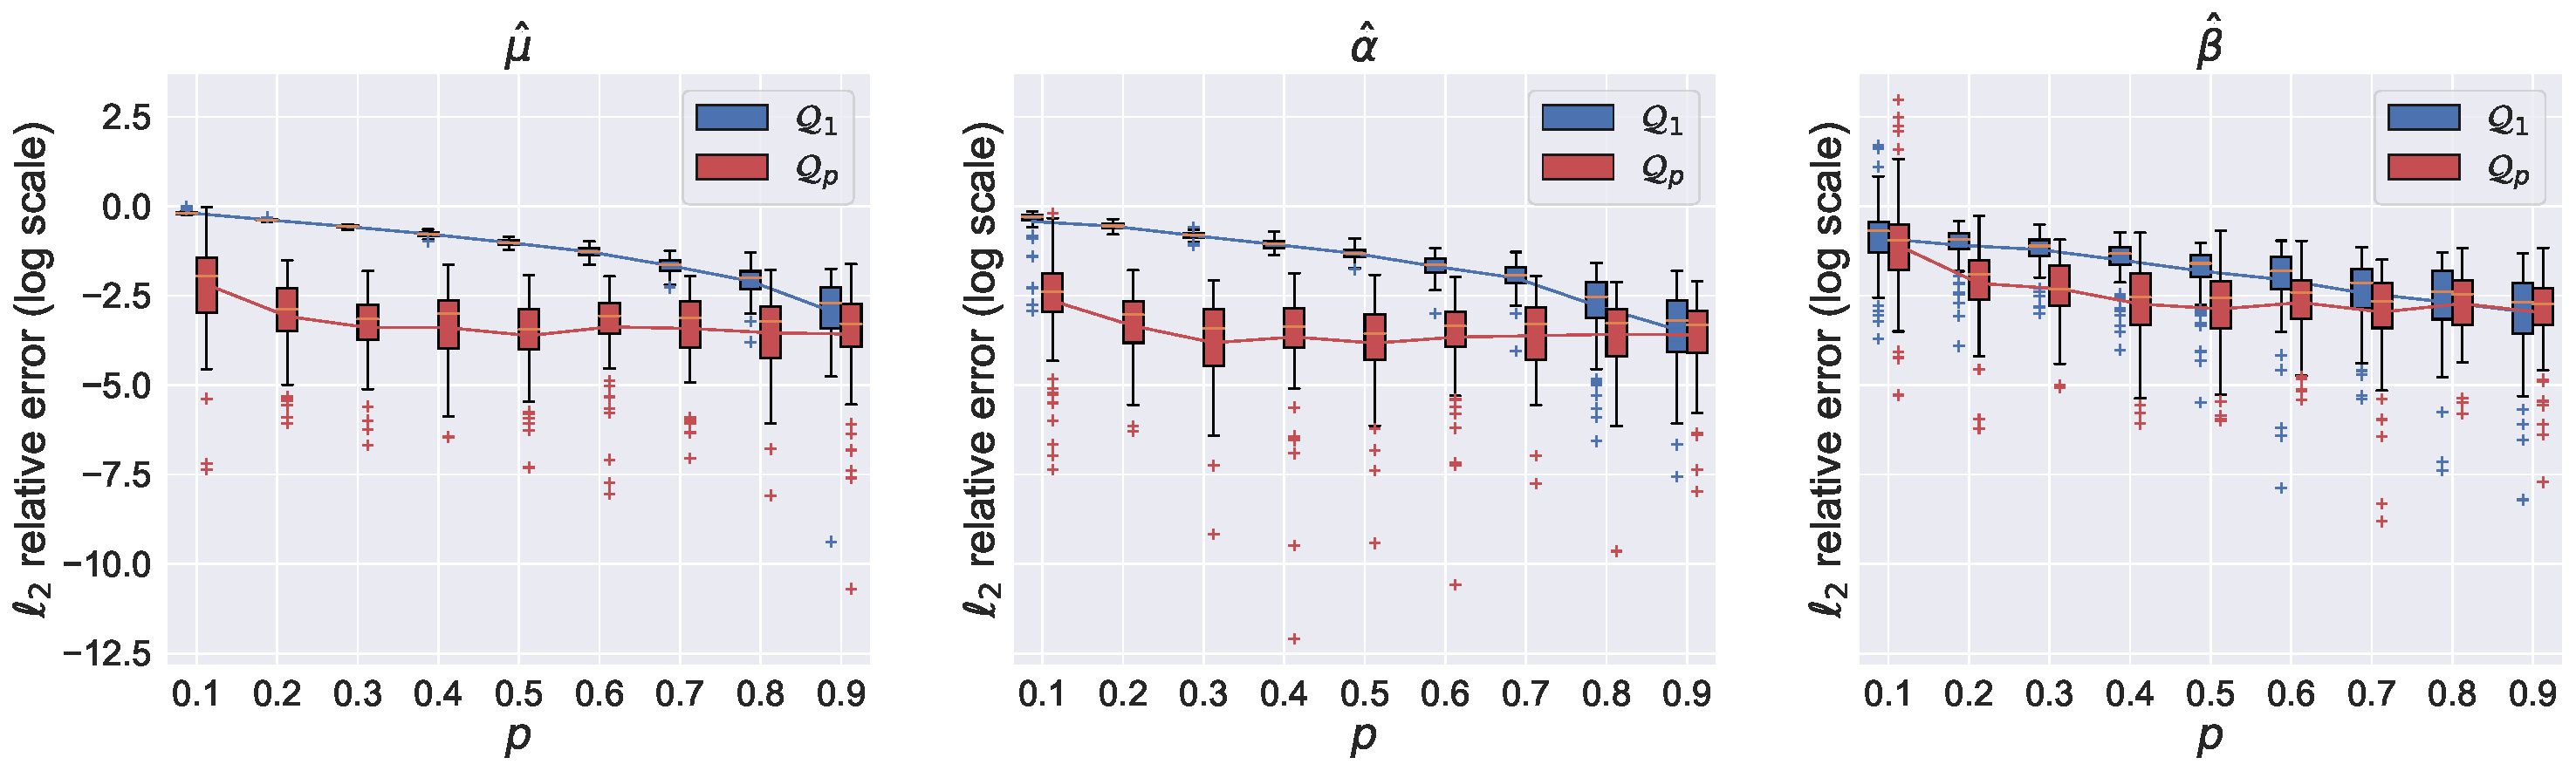
\includegraphics[width=1.0\textwidth]{images/chapter5/l2_error_same_information.pdf} 
        \caption{Boxplots of $\ell_2$ relative error on log-scale with respect to level of thinning $p$. Estimations for each parameter for estimation on the correct thinned model (red boxes) and on the model without accounting for thinning (blue boxes).
        }
        \label{fig:chap5_l2_error_same_information}
    \end{figure}

    \subsection{$p$-thinning as a subsampling method}\label{sec:chap5_subsampling_numerical}
    
    In this section, we assume that we dispose of a single observation $H$ of a Hawkes process for the same parameters:
    \[\mu = 1.25\,,\quad \alpha = 0.5\,,\quad \beta = 1.5\,,\]
    and we consider a observation window of $[0, 50]$.
    The lack of multiple repetitions and the small window size tend to negatively affect estimation procedures for point processes.

    A common practice to improve estimations in such contexts is to considered a penalised version of the to-be-optimised function, in our case, the spectral log-likelihood (Equation~\eqref{eq:chap5_spectral_ll}). 
    We define then the $\ell_2$-penalised spectral log-likelihood, for any penalisation parameter $L\geq0$, as:
    \begin{equation}\label{eq:chap5_penalised_ll}
        \ell_{T}(\theta) - L \|\theta\|_2 \,.
    \end{equation}
    A penalised estimator can then by obtained by maximising this quantity.
    In this penalised setting, we will illustrate how combining the $\ell_2$ penalisation with a subsampling procedure by thinning provides better results than other approaches.

    As our work in this chapter concerns mainly the study of spectral approaches, we will solely take into consideration estimators obtained through such means.
    We will compare then four estimators:
    
    \begin{itemize}
        \item $\hat \theta$: the estimator obtained by maximising the non-penalised spectral log-likelihood (Equation~\eqref{eq:chap5_spectral_ll}) on the single observation $H$.
        \item $\hat \theta^L$: the estimator obtained by maxising the penalised spectral log-likelihood (Equation~\eqref{eq:chap5_penalised_ll}) on the single observation $H$.
        \item $\hat \theta^L_{partition}$: we partition the observation window $[0,T]$ in $I$ equally sized intervals: \[\left[\frac{iT}{I}, \frac{(i+1)T}{I}\right]\,,\] for $i=1:I-1$. For each window, we obtain a penalised estimator by maximising Equation~\eqref{eq:chap5_penalised_ll}, and finally we obtain $\hat \theta^L_{partition}$ by averaging all estimations. This is similar to subsampling by means of covering regions \parencite{Possolo1991, Politis1999, Guan2007}.
        \item $\hat \theta^L_{thinning}$: we perform $S$ different thinning procedures for a fixed $p\in(0,1)$ providing the $p$-thinned observations $H_1, \ldots, H_S$ of $H$. For each $H_s$, we obtain a penalised estimation by maximising Equation~\eqref{eq:chap5_penalised_ll} on the statistical model $\mathcal{Q}_p$ and we obtain $\hat \theta^L_{thinning}$ by averaging all estimations.
    \end{itemize}

    $\hat \theta^L_{partition}$ corresponds to a common practice in point processes theory used to split an observation into multiple samples, which is particularly useful for large values of $T$.

    Our proposed estimator $\hat \theta^L_{thinning}$ can be seen as an estimator obtained through a subsampling procedure, similar to the Bernoulli subsampling scheme (see for example \textcite[Chapter 3.2]{Sarndal2003}). 
    
    We will be focusing on studying the efficiency of all four methods and so we will be considering the following grids for the hyper-parameters $I, p$ and $L$:
    \[I\in\{2,3,4,5\}\,,\quad p\in\{0.1, \ldots, 0.9\}\,,\quad L\in\{10^{-6}, 10^{-5}, \ldots, 10^2\}\,.\]
    Concerning the subsampling parameter of $\hat \theta^L_{thinning}$, we fix it at $S=3$ but let us remark that all presented results are consistent for other values of $S$.
    Proposing a model selection procedure to choose the optimal hyper-parameters $I, p, L$ is out of the scope of this work, 
    so we solely present the best estimators obtained through each method in the sense of the relative $\ell_2$ error with respect to the true parameters of the model.

    Figure~\ref{fig:chap5_l2_error_subsampling} represents the $\ell_2$ relative error for each estimator over 1000 different simulations. 
    We ordered all curves so that the error of our proposed estimator $\hat \theta^L_{thinning}$ is shown in ascending order.

    \begin{figure}[!ht]
        \centering
        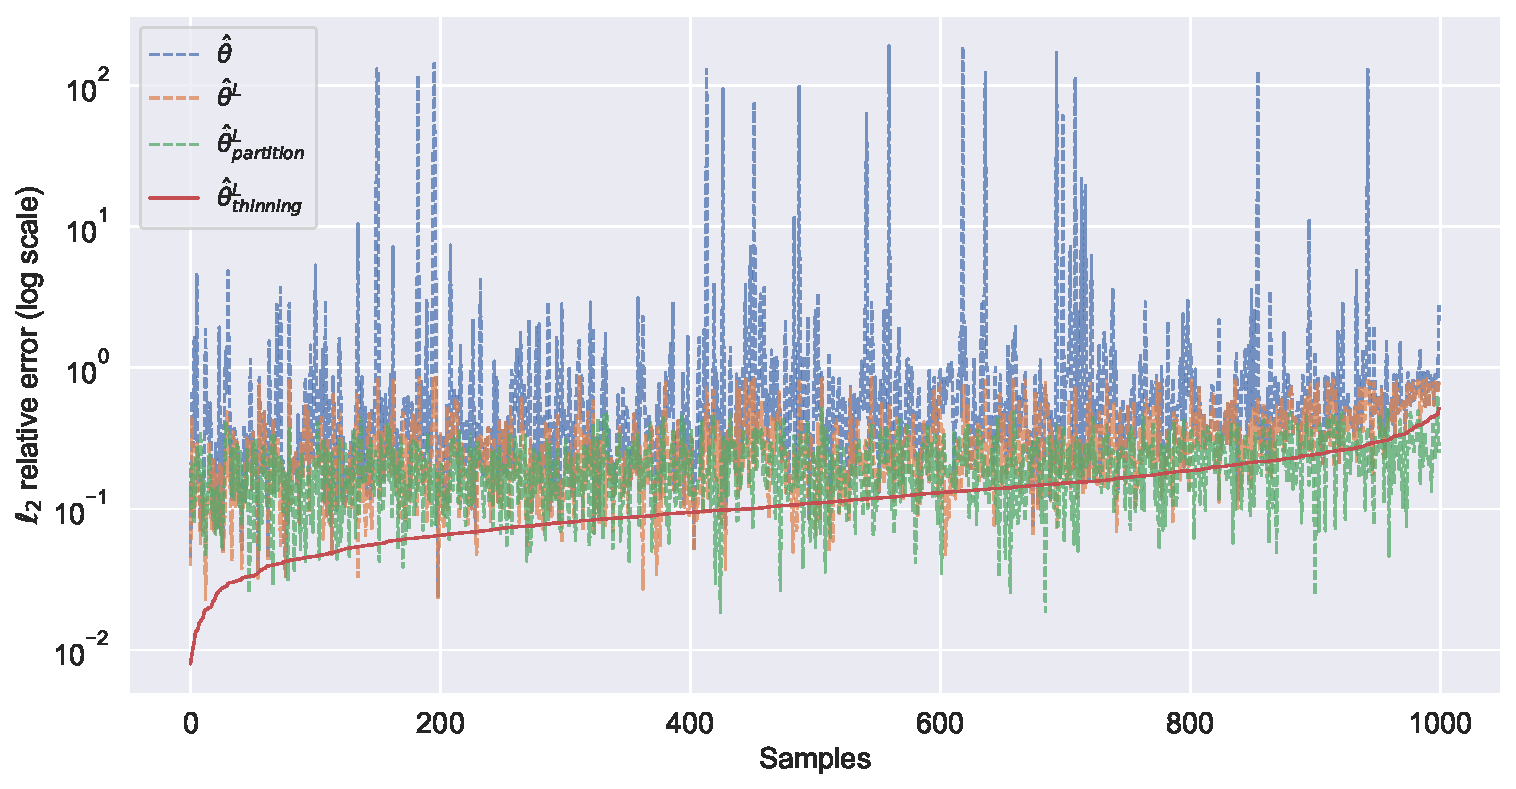
\includegraphics[width=1.0\textwidth]{images/chapter5/l2_error_subsampling.pdf} 
        \caption{$\ell_2$ relative error of all four estimators without penalisation (blue), with penalisation (orange), with penalisation and subsampling by partition (green) and our proposed method with penalisation and subsampling by thinning (red).
        1000 independent samples are shown and errors are sorted so to display the error of $\hat \theta^L_{thinning}$ in ascending order. 
        }
        \label{fig:chap5_l2_error_subsampling}
    \end{figure}

    We can initially notice that all other estimations (dashed lines) have in general higher $\ell_2$ errors than our proposed method.
    This can be confirmed in Table~\ref{tab:chap5_subsampling_table} displaying the proportion of times that each estimator outperformed the others.

    \begin{table}[!ht]
        \begin{center}  
            \centering
            \begin{tabular}{c|cccc|c}
                \multirow{2}{*}{Estimator} & \multicolumn{4}{c|}{MSRE} & \multirow{2}{*}{$\%$ best}\\
                & $\hat \mu$ & $\hat \alpha$ & $\hat \beta$ & $\hat \theta$ \\
                \midrule
                $\hat \theta$ & 0.18 & 0.13 & $5.14 \times 10^{2}$ & $2.85\times 10^{2}$ & 1\%\\
                $\hat \theta^L$ & 0.12 & 0.09 & 0.13 & 0.12 & 6.7\%\\
                $\hat \theta^L_{partition}$ & 0.08 & 0.07 & 0.04 & 0.05 & 22.3\%\\
                $\hat \theta^L_{thinning}$ & 0.03 & 0.04 & 0.02 & 0.02 & 70\% \\
            \end{tabular}
            \caption{Mean Square Relative Error of each estimator for each parameter $(\mu, \alpha, \beta)$ along with the MSRE of $\theta$.
            Last column shows the proportion of times that each estimator achieves the lower relative $\ell_2$ error accross all 1000 simulations.}
            \label{tab:chap5_subsampling_table}
        \end{center}
    \end{table}

    The non-penalised method provides by far the weakest estimator with a notably high MSRE when estimating $\beta$, which is consistently known as the hardest parameter to estimate in other parametric inference settings (see \textcite{Lemonnier2014} discussion on non-concavity for log-likelihood).

    The three penalised methods greatly improve the estimations, in particular for $\beta$, significantly reducing MSRE all around.
    We notice that the lowest MSRE are obtained by our thinning method, with it being in most scenarios the best method all around. 
    This is a testimony of the advantages of the subsampling and penalisation procedure that we propose in this work.


    % \begin{table}[h!]
    %     \begin{center}  
    %         \centering
    %         \begin{tabular}{c|ccc|cccc|c}
    %             \multirow{2}{*}{Estimator} & \multicolumn{3}{c|}{Average estimations} & \multicolumn{4}{c|}{RMSE} & \multirow{2}{*}{$\%$ best}\\
    %             & $\hat \mu$ & $\hat \alpha$ & $\hat \beta$ & $\hat \mu$ & $\hat \alpha$ & $\hat \beta$ & $\hat \theta$ \\
    %             \midrule
    %             $\hat \theta$ & 1.17 & 0.51 & 6.57 & 0.28 & 0.03 & $1.15 \times 10^{3}$\\
    %             $\hat \theta^L$ & 1.15 & 0.53 & 1.25 & 0.19 & 0.02 & 0.29\\
    %             $\hat \theta^L_{partition}$ & 1.04 & 0.56 & 1.49 & 0.12 & 0.02 & 0.08\\
    %             $\hat \theta^L_{thinning}$ & 1.16 & 0.52 & 1.46 & 0.05 & 0.01 & 0.04\\
    %         \end{tabular}
    %         \caption{.}
    %         \label{tab:chap5_subsampling_table}
    %     \end{center}
    % \end{table}


\section{Discussion}
    In this chapter, we leverage the spectral theory of point processes to present a parametric estimation procedure for thinned versions of univariate Hawkes processes.
    A first motivation for studying this model concerns the study of imperfect data and we showcase the efficiency of the spectral analysis to tackle such problems.
    This approach does not come without some issues, as we show that the underlying spectral density model is not identifiable without additional information on the parameter to be estimated.
    However, we highlight the efficiency of our estimation method once that identifiability is recovered, which is a step towards improving estimation in situations with eventual missing event times.
    Our second contribution is to make use of thinning as a tool to perform subsampling in scenarios with small sample sizes and low observation windows. 
    By introducing a penalisation version of the spectral log-likelihood and combining this with subsampling, we demonstrate that we are able to significantly improve estimations. 
    This is encouraging for real world situations, such as in health or biology, where acquiring sizeable quantities of data is difficult.

    The main extension of our work would be to adapt our methods to higher dimensional data in order to consider multiple inter-connected phenomena, for instance in epidemiology, social interaction or neurobiology.
    In particular, our idea of introducing a subsampling approach for penalised optimisation methods is highly motivated by the high interest in Lasso approaches for multivate point processes.
    This kind of regularisation is used in order to determine a sparse matrix of interaction for high-dimensional networks where only few connections between individuals exist.
    As these approaches tend to require a high amount of information or samples in order to perform well, adapting our subsampling scheme would allow to make more them more accessible.
    A last avenue of exploration would be to propose a model selection procedure adapted to spectral approaches in order to choose the hyper-parameters of the penalised and subsampling methods in practical contexts where information on the real parameters is unavailable.
    %A last avenue of exploration would be to develop the spectral theory for more general Hawkes processes that are used in practice, either with more complicated kernel functions or for non-linear versions allowing for inhibiting effects.



\begin{subappendices}
    \section{Proof of Proposition~\ref{prop:chap5_spectral_thinning}}\label{appendix:chap5_proof_spectral_thinning}
        Let $H_p$ be a $p$-thinning of a stationary point process $H$ admitting a Bartlett spectrum $\Gamma^H$ and a spectral density function $f^H$.
        The stationarity of $H_p$ is given by the fact that the variables $(Z_k)_{k\in\ZZ}$ are i.i.d. and so for any integer $r$, 
        for any $B_1\ldots, B_r \in\mathcal{B}^c$, 
        the random vector $(N_p(B_k)_{k=1:r})$ has the same distribution as $(N_p(B_k+t)_{k=1:r})$,
        for any $t\in\RR$.
        We will then denote $\Gamma^{H_p}$ and $f^{H_p}$ respectively the Bartlett spectrum and spectral density function of $H_p$

        In order to establish Equation~\eqref{eq:chap5_spectral_thinning}, we will leverage Theorem~\ref{th:chap5_spectral_marked}.
        We consider then the marked version $\bar H$ of $H$ where the marks $Z_k$ are i.i.d. Bernoulli distributions with common probability $p$.

        Let $\varphi, \psi \in \mathcal{S}$, we define, for all $x,z\in\RR\times\{0,1\}$, the functions:
        \[\varphi^\star(x,z) = \varphi(x)z\,,\qquad \psi^\star(x,z) = \psi(x)z\,.\]

        Let us verify that these functions verify the conditions of Theorem~\ref{th:chap5_spectral_marked}. 
        Without lose of generality, we will work uniquely with $\varphi^\star$, as the arguments are exactly the same for $\psi^\star$.
        
        For any $x\in\RR$, $\varphi^\star(x, Z) = \varphi(x)Z$ for Z a Bernoulli distribution of parameter $p$.
        It follows that $\varphi^\star(x, Z)$ admits a first and second order moment, and as $\varphi\in\mathcal{S}$, 
        $\varphi(x)Z$ is integrable and twice integrable, which shows that:
                \[
                \int_{\RR}{\EE\left[|\varphi^\star(x, Z)|\right]\dd x} < +\infty\,,\qquad 
                \int_{\RR}{\EE\left[\varphi^\star(x, Z)^2\right]\dd x} < +\infty\,.
                \]
        Furthermore, for any $x\in\RR$, $\bar \varphi(x) = \varphi(x)\EE[Z] = p \varphi(x)$,
        and so, as the Schwartz space is closed under scalar mutliplication, it follows that $\bar \varphi\in\mathcal{S}$.

        We can then apply Equation~\eqref{eq:chap5_marked_spectrum} to our marked process $\bar H$. 
        For this, let us notice that:
        \[
            \sum_{k\in\ZZ}{\varphi^\star(T_k, Z_k)} = \sum_{k\in\ZZ}{\varphi(T_k)Z_k} = \int_{\RR}{\varphi(t) H_p(\dd t)}\,,
        \]
        with the same expression holding for $\psi^\star$ and $\psi$. 
        So, the left-hand side of Equation~\eqref{eq:chap5_marked_spectrum} reads:
        \begin{align}
            \Cov\left(\sum_{k\in\ZZ}{\varphi^\star(T_k, Z_k)}, \sum_{k\in\ZZ}{\psi^\star(T_k, Z_k)}\right) &=
            \Cov\left(\int_{\RR}{\varphi(t) H_p(\dd t)}, \int_{\RR}{\psi(t) H_p(\dd t)}\right) \nonumber\\
            &= \int_{\RR}{\tilde \varphi(\omega)\tilde \psi(-\omega)\,\Gamma^{H_p}(\dd\omega)}\,,\label{eq:chap5_leftside_proof_thinning}
        \end{align}
        where the last equality comes from Equation~\eqref{eq:chap5_bartlett_covariance}.

        For the left-hand side, let us remark that $\bar \varphi(x) = p \varphi(x)$ for any $x\in\RR$ and so, for any $\omega\in\RR$,
        \[
            \tilde {\bar \varphi}(\omega) = p \tilde \varphi(\omega)\,,
        \]
        and,
        \[\tilde \phi^\star(\omega, Z) = \tilde \phi(\omega)Z\,.\]

        The right-hand side of Equation~\eqref{eq:chap5_marked_spectrum} becomes:

        \begin{align}
            \int_{\RR}{\tilde {\bar\varphi} (\omega) \tilde{\bar \psi} (-\omega)\,\Gamma^H(\dd \omega)} 
        + &\int_{\RR}{\Cov\left( \tilde \varphi^\star(\omega, Z), \tilde \psi^\star (-\omega, Z)\,M_1(\dd \omega)\right)} \nonumber\\
        &= \int_{\RR}{p^2 \tilde {\varphi} (\omega) \tilde{\psi} (-\omega)\,\Gamma^H(\dd \omega)} 
        + \int_{\RR}{\tilde \varphi(\omega)\tilde \psi(\omega) \Cov\left(Z,Z\right)M_1(\dd \omega)} \nonumber\\
        &= \int_{\RR}{\tilde {\varphi} (\omega) \tilde{\psi} (-\omega)\,(p^2\Gamma^H(\dd \omega) + p(1-p) M_1(\dd \omega))}\,.\label{eq:chap5_rightside_proof_thinning}
        \end{align}

        By combining both sides (Equations~\eqref{eq:chap5_leftside_proof_thinning} and \eqref{eq:chap5_rightside_proof_thinning}) it follows that,
        for any $\varphi, \psi\in\mathcal{S}$:
        \[
            \int_{\RR}{\tilde \varphi(\omega)\tilde \psi(-\omega)\,\Gamma^{H_p}(\dd\omega)} = \int_{\RR}{\tilde {\varphi} (\omega) \tilde{\psi} (-\omega)\,(p^2\Gamma^H(\dd \omega) + p(1-p) M_1(\dd \omega))}\,.
        \]
        
        As this equality holds for any functions in the Schwartz space, by duality of the Fourier transform \parencite{Pinsky2008}, then,
        \[\Gamma_p = p^2 \Gamma + p(1-p) M_1\,,\]
        and as $M_1 = m_1 \ell_{\RR}$,
        \[f_p(\omega) = p^2 f(\omega) + p(1-p) m_1\,,\]
        which achieves the proof.



    \section{Proof of Proposition~\ref{prop:chap5_identifiability_thinning}}\label{appendix:chap5_proof_identifiability_thinning}

    Let $\theta = (\mu, \alpha, \beta, p)$ and $\theta' = (\mu', \alpha', \beta', p')$ be two admissible parameter for model $\mathcal{Q}$.

    In order to prove that model $\mathcal{Q}$ is identifiable if and only if one of four parameters is fixed, 
    we will begin by retrieving the system of Equations~\eqref{eq:chap5_nonidentifiable_parameters}
    and verify that it defines an admissible parameter for $\mathcal{Q}$.
    Subsequently we will verify that by fixing one parameter, we retrieve the identifiability of the model.
    
    We begin by assuming that $f_\theta = f_{\theta'}$.
    By Equation~\eqref{eq:chap5_spectral_exponential}, this equality reads:
    \[\forall \omega \in \RR,\quad 
    \frac{\mu p }{1-\alpha}\left(1 + p \frac{\beta^2 \alpha (2-\alpha)}{\beta^2(1-\alpha)^2 + 4 \pi^2 \omega^2}\right) = 
    \frac{\mu' p' }{1-\alpha'}\left(1 + p' \frac{{\beta'}^2 \alpha' (2-\alpha')}{{\beta'}^2(1-\alpha')^2 + 4 \pi^2 \omega^2}\right)\,.
    \]

    Let us remark that a sufficient condition for both sides to be equal, 
    for all $\omega \in \RR$,
    is that the following system of equations is verified:

    \begin{equation}\label{eq:chap5_system_identifiability}
        \begin{cases}
            \frac{\mu p }{1-\alpha} = \frac{\mu' p'}{1-\alpha'}\\
            p \beta^2 \alpha(2-\alpha) = p' {\beta'}^2 \alpha'(2-\alpha')\\
            \beta (1-\alpha) = \beta' (1-\alpha')\,,
        \end{cases}
    \end{equation}
    as this would mean that the three constants (w.r.t. $\omega$) in both sides are equal.
    In fact this is also a necessary condition as the three equalities can be retrieved for $f(0)$, $\lim_{\omega\to+\infty}{f(\omega)}$ and $f(1)$
    and combining the equations.

    Let $\kappa\in(0, 1/p)$ and $p' = \kappa p$, which reduces the system of Equations~\eqref{eq:chap5_system_identifiability} to:

    \begin{subnumcases}{}
            \frac{\mu}{1-\alpha} = \frac{\mu' \kappa}{1-\alpha'}\label{eq:chap5_system_identifiability1}\\
            \beta^2 \alpha(2-\alpha) = \kappa {\beta'}^2 \alpha'(2-\alpha')\label{eq:chap5_system_identifiability2}\\
            \beta (1-\alpha) = \beta' (1-\alpha')\,,\label{eq:chap5_system_identifiability3}
    \end{subnumcases}

    As $\alpha > 1$, $\alpha'>1$, $\beta>0$ and $\beta'>0$, 
    Equation~\eqref{eq:chap5_system_identifiability3} can be expressed as:
    \[{\beta'}^2 = \frac{\beta^2(1-\alpha)^2}{(1-\alpha')^2}\,,\]
    and by replacing ${\beta'}^2$ in Equation~\eqref{eq:chap5_system_identifiability2}, we obtain:
    \begin{align}
        &\frac{\alpha (2-\alpha)}{(1-\alpha)^2} = \kappa \frac{\alpha' (2-\alpha')}{(1-\alpha')^2}\label{eq:chap5_alpha_equality} \\
        \iff\quad & \frac{1 - (1-\alpha)^2}{(1-\alpha)^2} = \kappa \frac{1 - (1-\alpha')^2}{(1-\alpha')^2}\nonumber \\
        \iff\quad & 1 + \frac{1}{\kappa}\left(\frac{1}{(1-\alpha)^2} - 1\right) = \frac{1}{(1-\alpha')^2}\nonumber\,,
    \end{align}
    and as $\alpha \in(0,1)$, the left-side term is positive and so:
    \[\alpha' = 1 - \frac{1}{\sqrt{1 + \frac{1}{\kappa}\left(\frac{1}{(1-\alpha)^2} - 1\right)}}\,.\]

    We can then obtain the explicit expressions of $\mu'$ and $\beta'$ with Equations~\eqref{eq:chap5_system_identifiability1} and \eqref{eq:chap5_system_identifiability3}
    providing the following system:
    
    \begin{equation}\label{eq:chap5_system_parameters}
        \begin{cases*}
            \mu' = \frac{\mu(1-\alpha')}{\kappa(1-\alpha)}\\
            \alpha' = 1 - \frac{1}{\sqrt{1 + \frac{1}{\kappa}\left(\frac{1}{(1-\alpha)^2} - 1\right)}}\\
            \beta' = \beta \frac{1-\alpha}{1-\alpha'}\\
            p' = \kappa p
        \end{cases*}
        \quad\iff\quad
        \begin{cases}
            \mu' = \frac{\mu}{\kappa(1-\alpha)\sqrt{1 + \frac{1}{\kappa}\left(\frac{1}{(1-\alpha)^2} - 1\right)}}\\
            \alpha' = 1 - \frac{1}{\sqrt{1 + \frac{1}{\kappa}\left(\frac{1}{(1-\alpha)^2} - 1\right)}}\\
            \beta' = \beta (1-\alpha) \sqrt{1 + \frac{1}{\kappa}\left(\frac{1}{(1-\alpha)^2} - 1\right)}\\
            p' = \kappa p\,.
        \end{cases}
    \end{equation}
    
    To verify that, for any $\kappa\in(0,1/p)$, parameter $\theta' = (\mu', \alpha', \beta', p')$ is an admissible parameter,
    we have to make sure that $\theta' \in \Theta = \RR_{>0}\times (0,1) \times \RR_{>0} \times (0,1)$.
    Let $\theta = (\mu, \alpha, \beta, p)\in\Theta$, $\kappa\in(0,1/p)$ and $\theta'$ defined by Equations~\eqref{eq:chap5_system_parameters}.
    For such a $\kappa$, $p'\in(0,1)$ is immediately verified.

    The rest of the conditions are verified if and only if: 
    \[\sqrt{1 + \frac{1}{\kappa}\left(\frac{1}{(1-\alpha)^2} - 1\right)} > 1 \iff \frac{1}{(1-\alpha)^2} - 1 > 0\\,.\]
    This is immediate as $\alpha\in(0,1)$ and so $\theta'\in\Theta$. 
    From Equations~\eqref{eq:chap5_system_parameters}
    we can see that $\theta'=\theta$ and we've proven that $f_\theta = f_{\theta'}$,
    so model $\mathcal{Q}$ is not identifiable.

    Lastly, let us show that if any of the four parameters is known then the model defined by the remaining triplet is identidiable.
    By considering the previously established equations (see Equations~\eqref{eq:chap5_alpha_equality} and \eqref{eq:chap5_system_parameters}), 
    we know that for $\theta = (\mu, \alpha, \beta, p)\in\Theta$ and $\theta' = (\mu', \alpha', \beta', p')\in\Theta$:
    \begin{equation}\label{eq:chap5_system_fixed}
        f_{\theta} = f_{\theta'} \quad\iff\quad 
        \begin{cases*}
            \mu' = \frac{\mu(1-\alpha')}{\kappa(1-\alpha)}\\
            \frac{\alpha (2-\alpha)}{(1-\alpha)^2} = \kappa \frac{\alpha' (2-\alpha')}{(1-\alpha')^2}\\     
            \beta' = \beta \frac{1-\alpha}{1-\alpha'}\\
            p' = \kappa p
        \end{cases*}\,.
    \end{equation}
    \begin{itemize}
        \item If $\mu = \mu'$, the system of Equations~\eqref{eq:chap5_system_fixed} reduces to:
        \begin{equation*}
            \begin{cases*}
                \kappa = \frac{(1-\alpha')}{(1-\alpha)}\\
                \kappa \frac{\alpha' (2-\alpha')}{(1-\alpha')^2} = \frac{\alpha (2-\alpha)}{(1-\alpha)^2}\\     
                \beta' = \frac{\beta}{\kappa}\\
                p' = \kappa p
            \end{cases*}\quad\iff\quad
            \begin{cases*}
                \kappa = \frac{(1-\alpha')}{(1-\alpha)}\\
                \frac{\alpha' (2-\alpha')}{(1-\alpha')} = \frac{\alpha (2-\alpha)}{(1-\alpha)}\\     
                \beta' = \frac{\beta}{\kappa}\\
                p' = \kappa p
            \end{cases*}\,.
        \end{equation*}

        As $\alpha\in(0,1)$ and $\alpha'\in(0,1)$, the second equation implies that $\alpha=\alpha'$ and so $\kappa=1$ and $\beta'=\beta$.

        \item If $\alpha = \alpha'$, the second equation in \eqref{eq:chap5_system_fixed} implies directly that $\kappa=1$ and so all other equalities follow.
        \item If $\beta = \beta'$, the third equation in \eqref{eq:chap5_system_fixed} implies that $\alpha=\alpha'$ and by the previous point all other equalities hold.
        \item If $p = p'$, $\kappa=1$ and the rest of equalities are verified.
        
        This shows that whenever one of the parameters is fixed, $f_\theta = f_{\theta'}$ implies $\theta = \theta'$. This achieves the proof.

    \end{itemize}



\end{subappendices}


\chapter{Discussion}

% {Idea 1 (simple):}
% \begin{itemize}
%     \item Contributions part by part, chapter by chapter with insistence on questions asked before
%     \item Perspectives in bullet points
% \end{itemize}

% \textbf{Idea 2 (similar but less scholar):}
% \begin{itemize}
%     \item A short explanation of thesis goals and achievements
%     \item First half contributions and perspectives
%     \item Second half contributions and perpectives
% \end{itemize}


% \textbf{Idea 3 (very scholar):}
% \begin{itemize}
%     \item Chapter by chapter summaries of contributions
%     \item Chapter by chapter perspectives
% \end{itemize}

% The goal of this thesis is to provide an overall insight of the difficulties of studying different extensions of the Hawkes process model.
% In the spirit of contributing to the study of extensions to the Hawkes process model, our contribution throughout this the
% The results presented here

%Our work in this thesis consisted in providing novel statistical tools for the analysis of the Hawkes process model in the frequentist parametric setting.
This thesis provides novel statistical tools for analysing the Hawkes process model within the frequentist parametric framework.
Our contributions intend to provide partial answers to the questions presented in Section~\ref{sec:chap0_outline}.
As emphasized throughout this manuscript, our main goal is to propose inference paradigms to enhance the quality of estimations when working with temporal data.
To achieve this, we focused our study on two different submodels of the Hawkes process, either to analyse inhibition effects or to properly account for imperfect data observations.
In a general sense, we leveraged and adapted results through two different log-likelihood optimisation approaches to address this issues.
Our main intention was to serve as a stepping stone to motivate more in-depth research on these topics.
We conclude our work here with a discussion on our contributions and perspectives we think can contribute significantly in this field.

In the first part of this thesis, our work consisted in studying Hawkes processes exhibiting inhibition effects.
As exposed before, this model has been largely studied under many different perspectives in the literature, either from a non-parametric or a Bayesian point of view.
Our main contribution was to take the first step towards filling up a gap in the frequentist parametric setting by properly accounting for inhibition effects in both the univariate and multivariate settings (Chapters~\ref{chapter:univariate_inhibition} and \ref{chapter:multivariate_inhibition} respectively).
To do this, we adapted one of the most classical inference procedures in statistics, the maximum likelihood estimation.
We show that we are able to properly adapt this method under certain conditions, namely the monotony of the interaction function in the univariate setting or by introducing a mild assumption on the parameter space for the exponential kernel for multivariate processes.
As we focus mainly in the study of exponential kernels, for its practicality from a numerical sense, a natural extension of our work is to broaden our study to other parametrisation choices for either our kernels or even by considering time-evolving baseline intensities.
In the multivariate setting, we also brought into the light the identifiability issues that may appear where exciting and inhibiting effects may coexist, and to partially provide an answer to this problem we proposed an observational sufficient condition to recover this property.
Further work in this direction would involve establishing necessary conditions for identifiability on the adjacency matrix support or on the relative proportion of inhibition to excitation.
Another avenue of exploration is study of statistical properties of our estimators, such as consistency and asymptotic normality, for example by leveraging the results of \textcite{Ogata1978} or by taking inspiration from the works of \textcite{Costa2020} on limit theorems for interaction functions with bounded support.
Our final contribution to this topic was introducing some ad-hoc methods to estimate the support on the interaction matrix for multivariate processes. 
We illustrated the numerical advantages of such a step specially by leveraging a resampling method introduced in \textcite{Reynaud2014}.
This allowed us to recover a sparse interaction matrix in a real-data context of neuronal activity analysis.
This is a vital step from an applicative point of view in order to obtain more explicative models and so proposing more robust approaches will greatly benefit this field.
We belive this is a promising research field with novel contributions as shown in the works of \textcite{Lotz2024} on sparsity tests for Hawkes processes.

The second half of this manuscript was consacrated to the study of imperfect data issued from Hawkes processes.
We concentrated our efforts on two different noised scenarios: the first one in Chapter~\ref{chapter:spectral_superposition} considered an observation of event times where additional points from an external process are observed, whereas Chapter~\ref{chapter:spectral_thinning} focused on observations with missing data points.
Our study was carried out by taking a spectral analysis approach and so a parallel contribution on our side was to display the attractive potential of leveraging such tools for the study of the point processes.
We proposed an estimation method by the maximisation of a spectral version of the log-likelihood which, as illustrated by our numerical experiments on synthetic data, perform particularly well when the underlying model is identifiable.
In our work, we provided different conditions to retrieve the identifiability of our models defined by the spectral density function. 
As shown, issues may arise depending on the choice of the kernel functions and the interaction matrix in the multivariate setting which derives from the spectral approach. Obtaining more general conditions to ensure that identifiability holds will be a huge improvement on the field, specially for higher dimensional processes.
Ensuring the asymptotic properties for our estimators is again an open question and would help to cement the usefulness of this method for studying more complex point processes dynamics. 
Encouragingly enough, there is a current growing interest in establishing such properties for spectral quantities, as exemplified in the works of \textcite{Yang2024}.
Our last contribution in this thesis was to present a numerical paradigm to improve spectral estimations on a difficult learning task with low samples and small observation windows.
We leveraged two common solution in statistics by introducing a Ridge penalised version of the spectral estimator with an additional layer of subsampling by thinning.
This allowed us to make use of our results on thinned data and we illustrated the improvement of this procedure on simulated data, with very encouraging results.
This subsampling framework has been studied in the literature with very recent works of \textcite{Cronie2024, Coeurjolly2024} and our method would largely benefit from model evaluation and model selection methods. 

% EXTENSIONS:
% \begin{itemize}
%     \item Other models for inhibition ? %positive part, better with others (and link with theoretical properties) but harder as implementation
%     \item Study theoretical properties of our models and estimators (identifiability, consistency, asymptotic normality)
    
%     \item Study other kernels and non-parametric settings through our approaches
    
%     \item Lasso penalisation for multivariate interaction matrix estimation
%     \item Evaluation methods and model selection through cross-validation thanks to spectral 
    
%     \item (Lien entre deux) Faux pos Faux neg (like in epidemics, combine both could help to model this dynamics)
%     %\item Applicaition links with spectral
%     %\item Prediciton ?? (maybe too small )
% \end{itemize}

%%%% Cambiar las refs 
%%%% Checar las bibliographies para updatear y quitar doublons
%%%% 
%%%% CHECAR LOS \cite[] y \citep[] PORQUE ALGUNOS NO CAMBIARON

\appendix

\backmatter

\printbibliography

\makebackcover

\end{document}
%%% Local Variables:
%%% flyspell-mode: 1
%%% ispell-local-dictionary: "french"
%%% End:
